% Chapter 4

\chapter{Results}
\label{chap:results}

\section{Turbulence-specific Post-processing}

In order to make available all of the turbulence-specific post-processing from a given simulation output of \texttt{PySPH} \parencite{ramachandran2021a}, generated through the \texttt{Application} class, a \texttt{TurbulentFlowApp} class was created. This class inherits from the \texttt{Application} class and adds additional post-processing attributes and methods, such as:

\begin{itemize}
	\item class attributes:
	\begin{itemize}
		\item number of interpolation points along each axis,
		\item kernel to be used for the interpolation, and the corresponding kernel radius,
		\item interpolation method,
		\item norm order to be used for the computation of the $1D$ energy spectrum (also referred to as the \textit{scalar energy spectrum}),
		\item expected slope for the $1D$ energy spectrum,
        \item type of FTLE field (either \textit{forward} or \textit{backward}),
	\end{itemize}
	
	\item class methods:
	\begin{itemize}
		\item \texttt{compute\_interpolated\_vel\_field}: to compute the interpolated velocity field at specified indices of the output files,
        \item \texttt{compute\_ek}: to compute the $1D$ energy spectrum from the corresponding interpolated velocity field,
        \item \texttt{compute\_ek\_slope}: to compute the slope of the $1D$ energy spectrum, using the \texttt{scipy.stats.linregress} function,
        \item \texttt{compute\_ftle}: to compute the FTLE (Finite-time Lyapunov Exponent) field, using the corresponding interpolated velocity field between two specific output files,
        \item plotter functions that can plot the $1D$ energy spectrum for a specific output file (along with a fit line), plot the evolution of the $1D$ energy spectrum over a range of output files, or plot the FTLE field.
	\end{itemize}
\end{itemize}

The derived class is also coded to log the details of the interpolator used, which includes details on the kernel, radius scale, problem dimension, and SPH equations involved in the interpolation scheme in the original \texttt{problem.log} file created by the default \texttt{Application} class. This enables the user to keep track of all of the simulation's relevant details, including its post-processing, in a single log file.

The following subsections detail the implementation of the energy spectrum and FTLE field computation and essential observations made from the same.


\subsection{Energy Spectral Density}
In order to compute the energy spectrum, the following steps are performed:

\begin{itemize}
    \item the velocity field is interpolated along a grid of uniformly spaced rectangular points,
    \item the velocity field is then transformed to Fourier space, using the \texttt{numpy.fft.fftn} function \parencite{harris2020array}, and subsequently normalised as given as
    \begin{equation}
        \hat{\vect{v_i}}(\vect{k}) = \frac{ fft\{ \vect{v_i}(\vect{r}) \} }{U_0 \times len(\vect{v_i})}
    \end{equation}
    where $U_0$ is a reference velocity and $\vect{v_i}$ is the $i^{th}$ component of the velocity field,
    \item the corresponding energy spectrum is then computed as
    \begin{equation}
        \vect{E_i}(\vect{k}) = \frac{1}{2} \hat{\vect{v_i}}^2
    \end{equation}
    \item the $1D$ energy spectrum $E(k)$ is then computed from the energy vector field $\vect{E_i}(k_x, k_y, k_z)$, by integrating it over the surface of a sphere of appropriate dimension between the limits $k=0$ and $k=k_{max}$, where $k_{max}$ is the maximum wavenumber of the energy spectrum, where 
    \begin{equation}
        k_{max} = round(1 + ceil(|(l_x, l_y, l_z)|/2))
    \end{equation}
\end{itemize}

The function to compute the $1D$ energy spectrum was coded using three different backends, namely, pure \texttt{python}, \texttt{numba} \parencite{Lam_Pitrou_Seibert_2015}, and \texttt{compyle} \parencite{compyle_pr_ab-proc-scipy-2020}.
The speedup results of the three implementations are shown in \figref{fig:espec-speedup} for $1D$, $2D$, and $3D$ velocity fields, respectively.

\begin{figure}[htbp!]
    \begin{subfigure}{7cm}
      \centering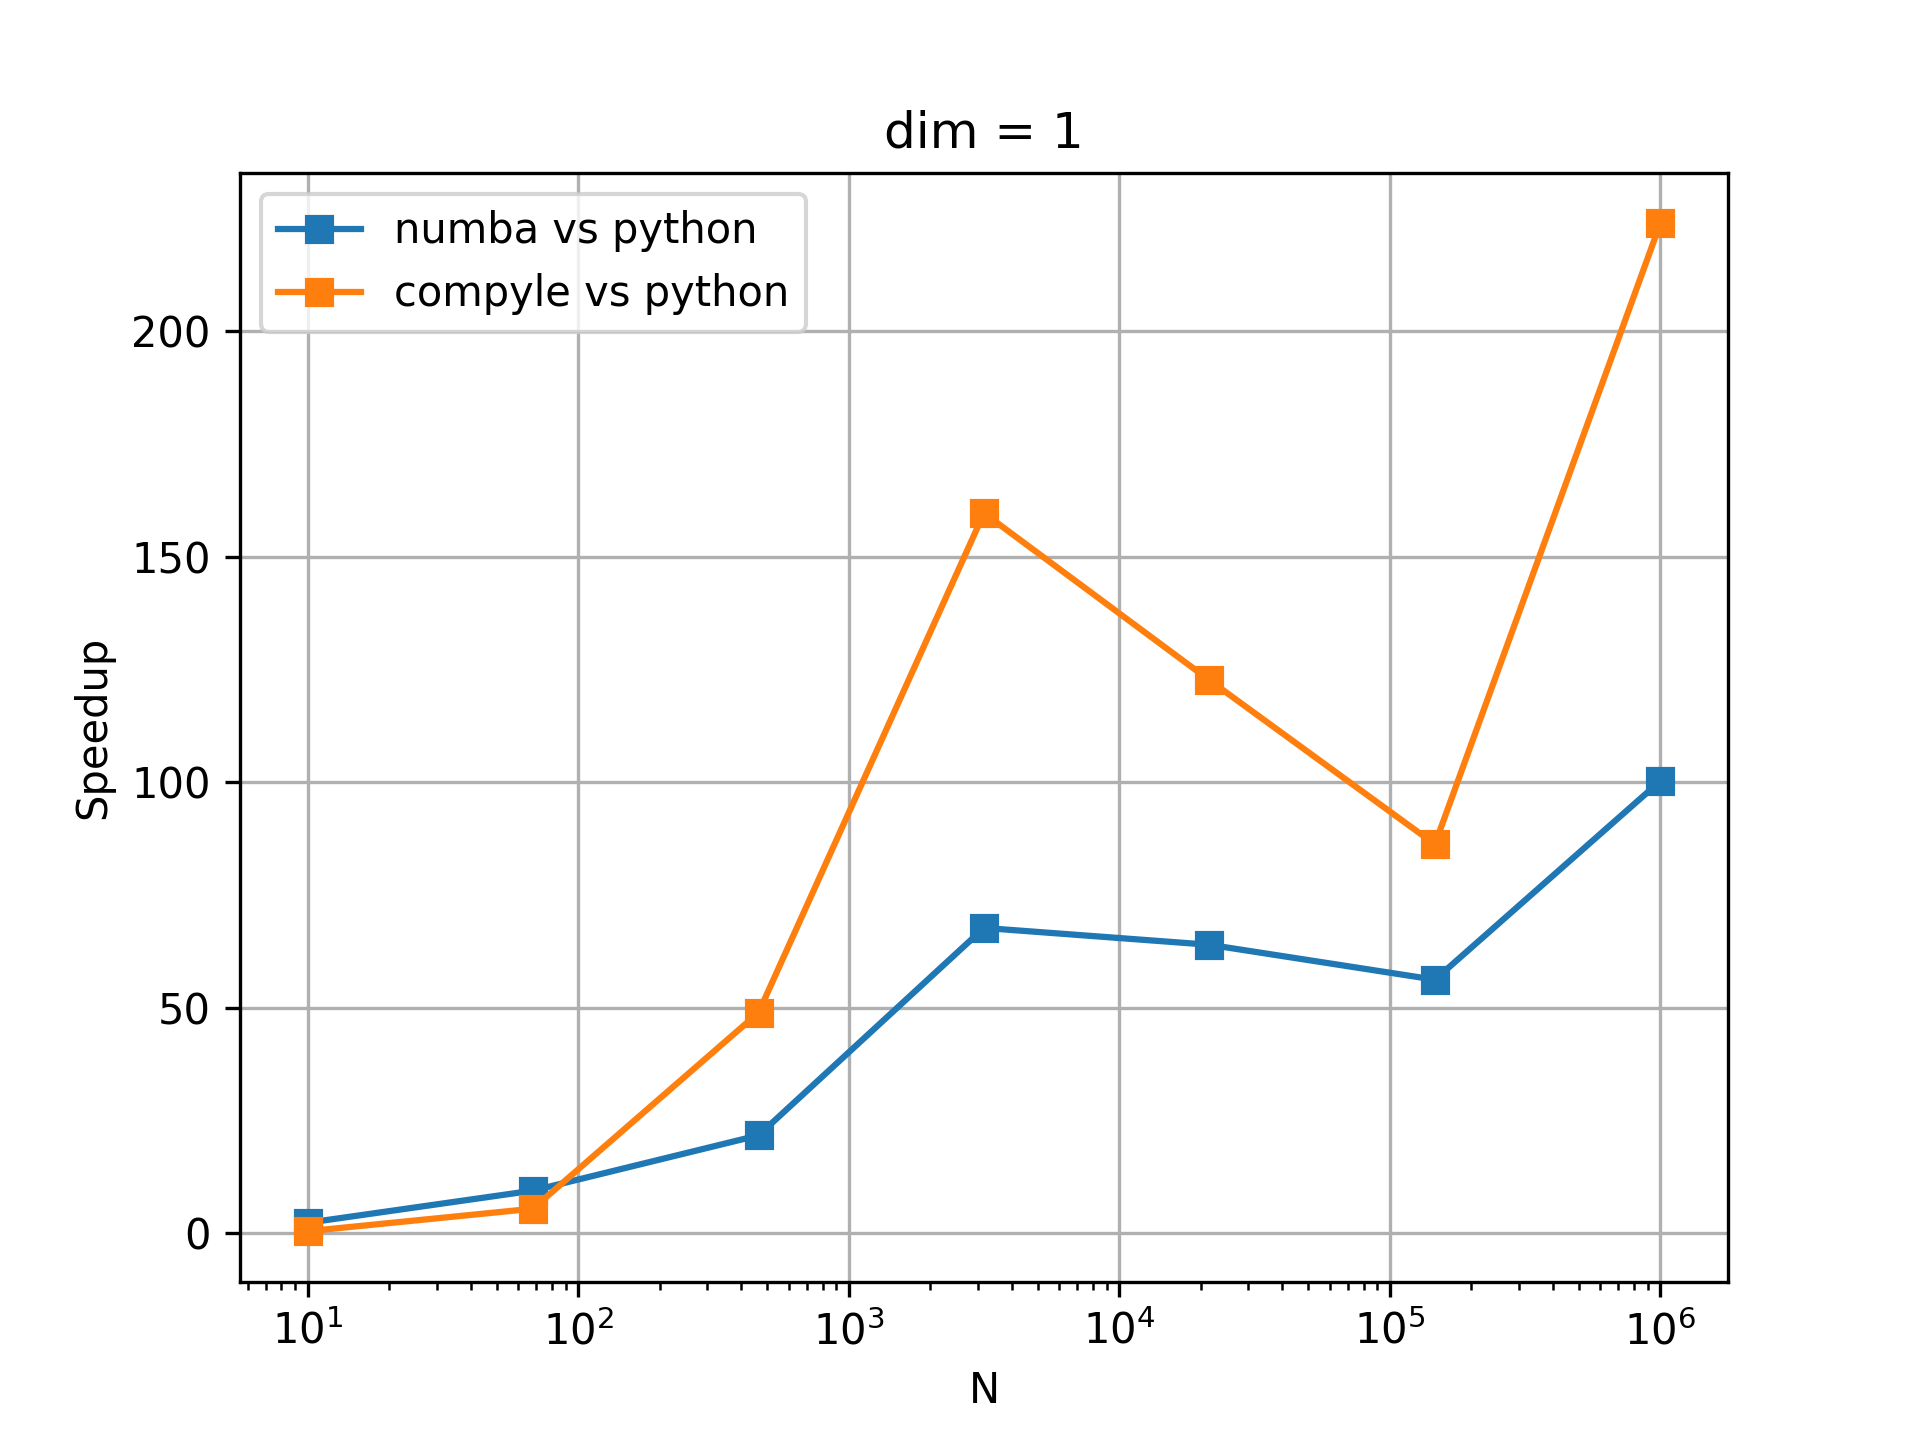
\includegraphics[width=6cm]{Code-Figures/espec_speedup_dim_1.png}
      \caption{$1D$ velocity field}
    \end{subfigure}
    \begin{subfigure}{7cm}
      \centering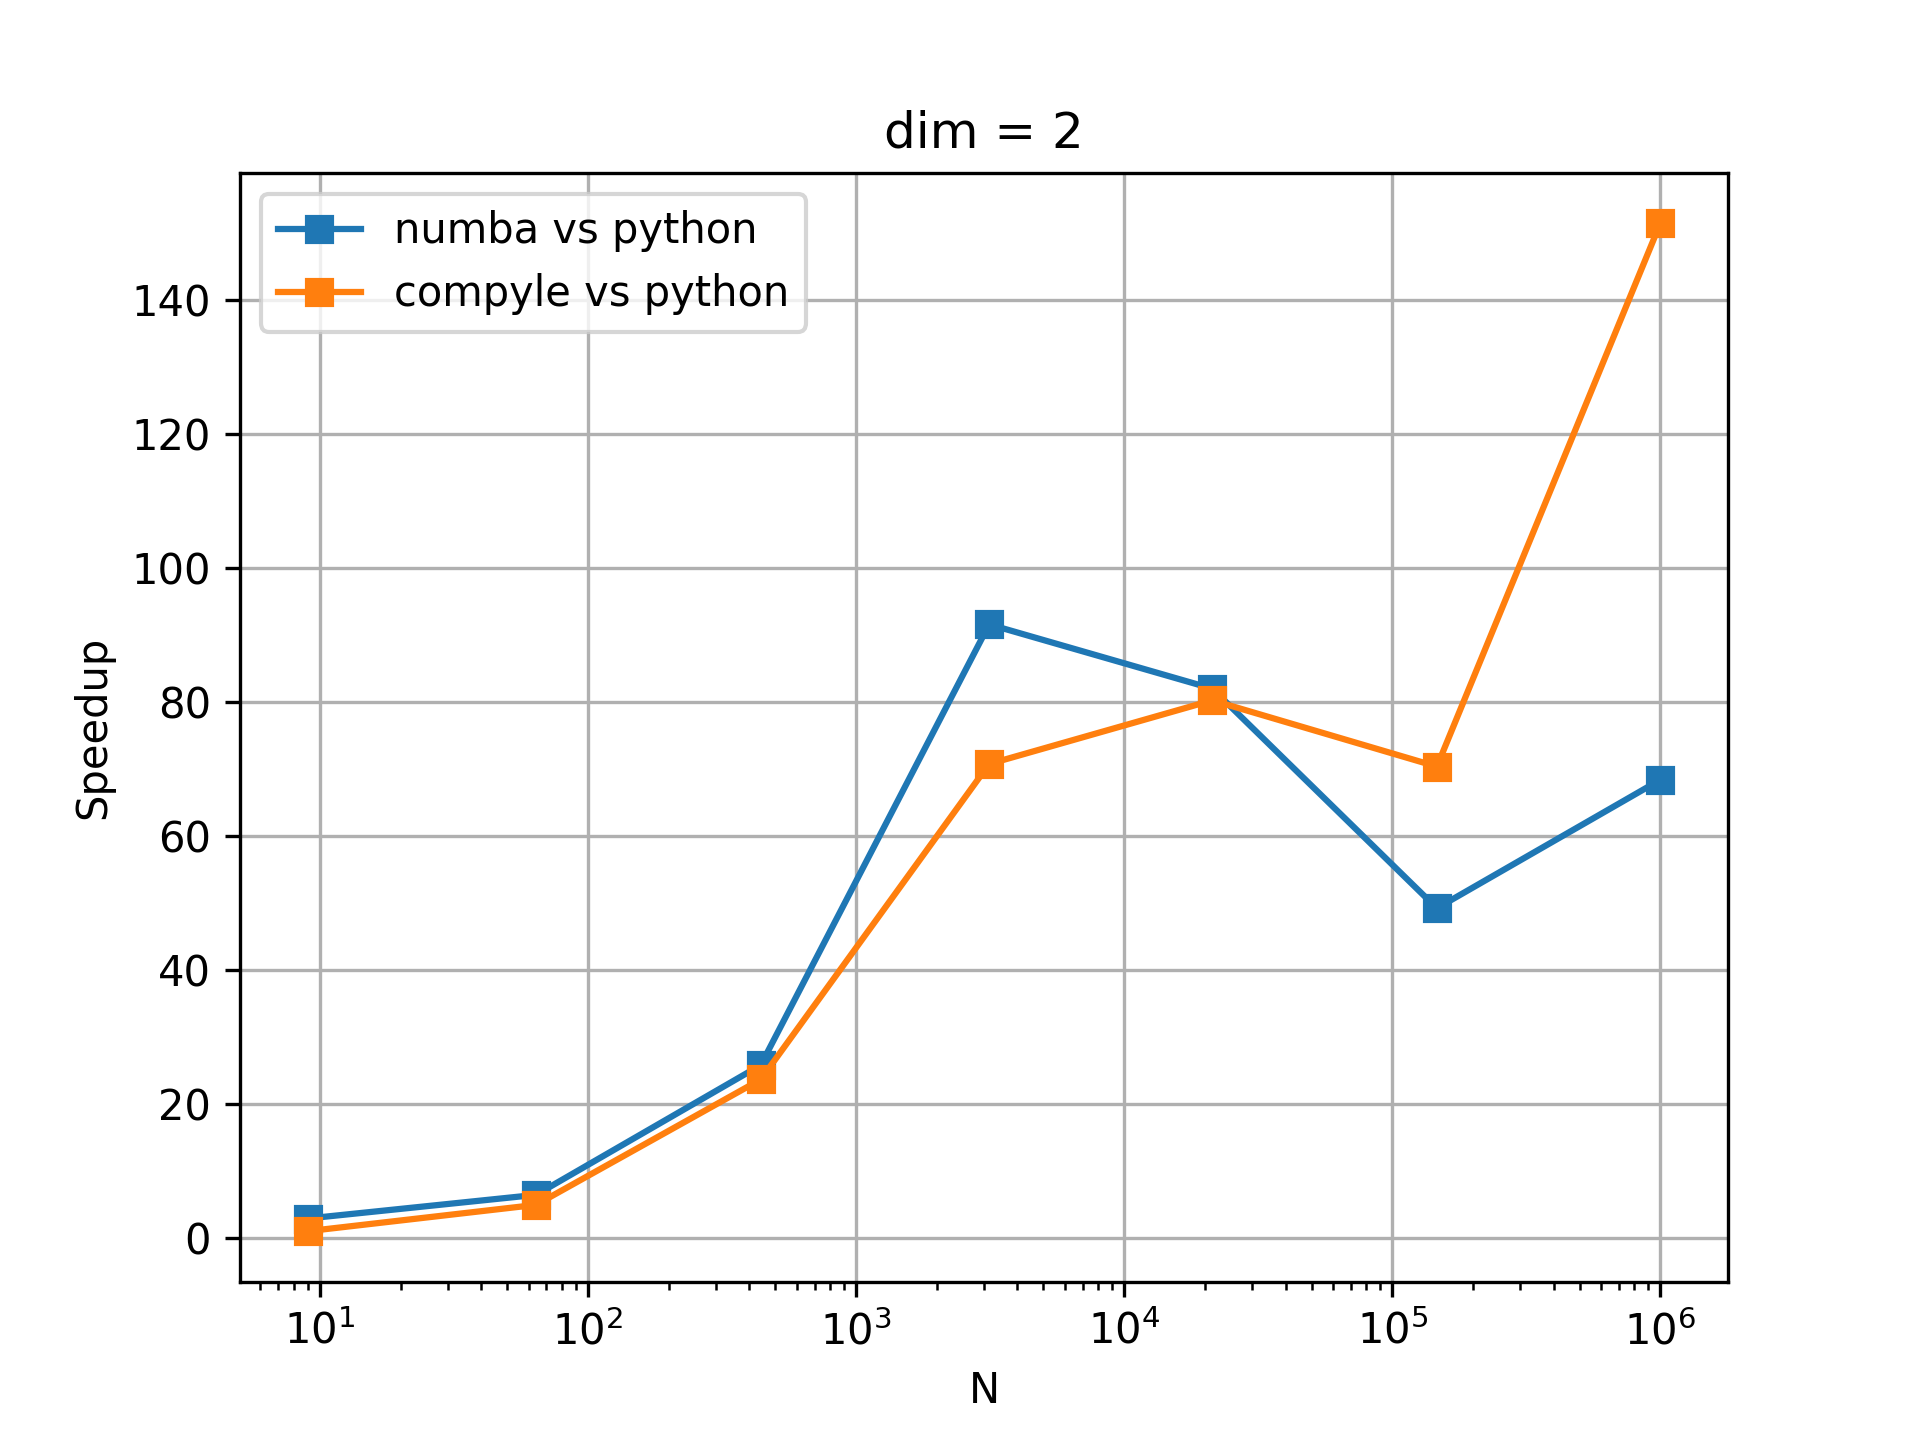
\includegraphics[width=6cm]{Code-Figures/espec_speedup_dim_2.png}
      \caption{$2D$ velocity field}
    \end{subfigure}
    \begin{subfigure}{7cm}
      \centering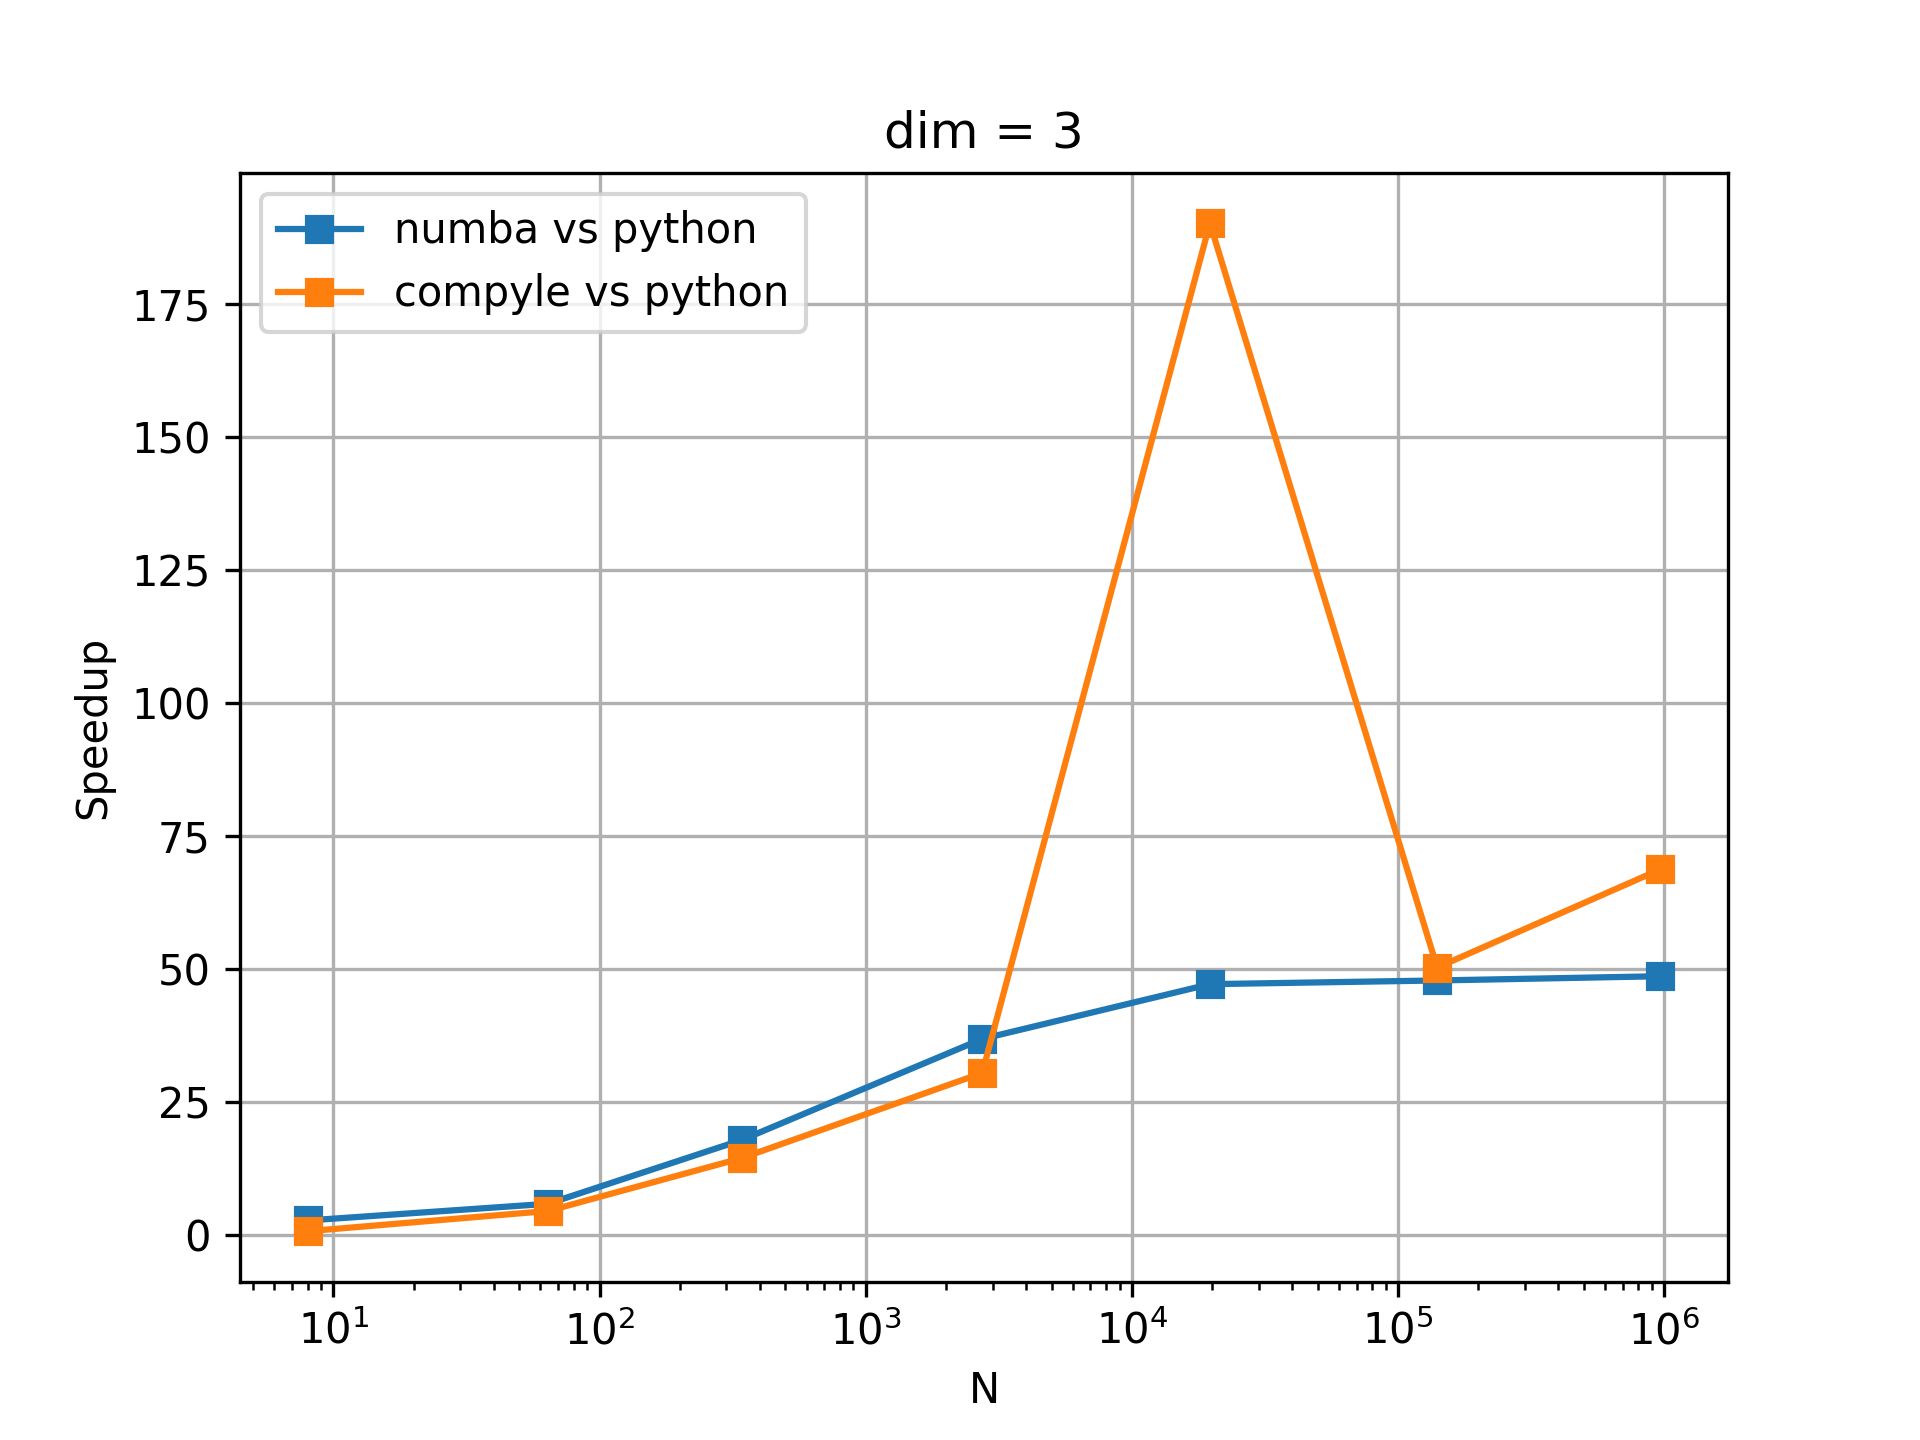
\includegraphics[width=6cm]{Code-Figures/espec_speedup_dim_3.png}
      \caption{$3D$ velocity field}
    \end{subfigure}
    \caption{Speedup of the $1D$ energy spectrum computation for various dimensions of the velocity field.}
    \label{fig:espec-speedup}
\end{figure}

The speedup plots show that the \texttt{numba} implementation is around $50-100\times$ faster than the pure \texttt{python} implementation. In comparison, the \texttt{compyle} implementation is around $80-150\times$ faster than the pure \texttt{python} implementation for various resolution scales. These trends are observed across all dimensions of the velocity field. The \texttt{compyle} implementation, in addition, to being faster than the \texttt{numba} implementation, also has the added advantage of not requiring any additional dependencies, which are not already required by \texttt{PySPH}, unlike the \texttt{numba} implementation, which requires the \texttt{numba} package to be installed separately. Hence, the \texttt{compyle} implementation was chosen for the final implementation of the $1D$ energy spectrum computation.

In order to test the code for correctness, the following test cases were devised. The velocity field for $1D$, is given as:
\begin{equation}
    v_x = - \sum_{i=1}^{N} i^{-\gamma} \cos(2 \pi i x),
\end{equation}
where, $N$ is the number of modes, and $\gamma$ is the decay rate of the modes.
For $2D$, the velocity field is given as:
\begin{equation}
    v_x = - \sum_{i=1}^{N} i^{-\gamma} \cos(2 \pi i x) \sin(2 \pi i y)
\end{equation}
\begin{equation}
    v_y = \sum_{i=1}^{N} i^{-\gamma} \sin(2 \pi i x) \cos(2 \pi i y).
\end{equation}
For $3D$, the velocity field is given as:
\begin{equation}
    v_x = - \sum_{i=1}^{N} i^{-\gamma} \cos(2 \pi i x) \sin(2 \pi i y) \sin(2 \pi i z)
\end{equation}
\begin{equation}
    v_y = \sum_{i=1}^{N} i^{-\gamma} \sin(2 \pi i x) \cos(2 \pi i y) \sin(2 \pi i z)
\end{equation}
\begin{equation}
    v_z = \sum_{i=1}^{N} i^{-\gamma} \sin(2 \pi i x) \sin(2 \pi i y) \cos(2 \pi i z).
\end{equation}
Since the energy in the flow field is a function of the square of the velocity, the corresponding decay rate in the energy spectrum will be $2\gamma$.

The first order of correctness involved running the energy spectral calculation for the above test cases, using only one mode ($N=1$) and zero decay rate ($\gamma=0$).

The vector energy spectral fields are shown in \figref{fig:espec-vector-fields-N1}. It should be noted that the plots are shown by shifting the energy spectrum such that the centre of the plot corresponds to the zero wavenumber. This is done since the energy spectrum is symmetric about the zero wavenumber, and hence, the plot is more informative when the zero wavenumber is at the centre of the plot. Here, it can be observed that in both the $1D$ and $2D$ cases, the energy spectrum peaks only for $k=1$ and is zero for every other wavenumber, indicating the nature of the velocity field, consisting of only one mode. 

The scalar energy spectral fields are shown in \figref{fig:espec-scalar-fields-N1}. As can be seen, the energy spectrum peaks only for $k=1$ and is zero for every other wavenumber for all dimensions.

\begin{figure}[htbp!]
    \begin{subfigure}{7cm}
      \centering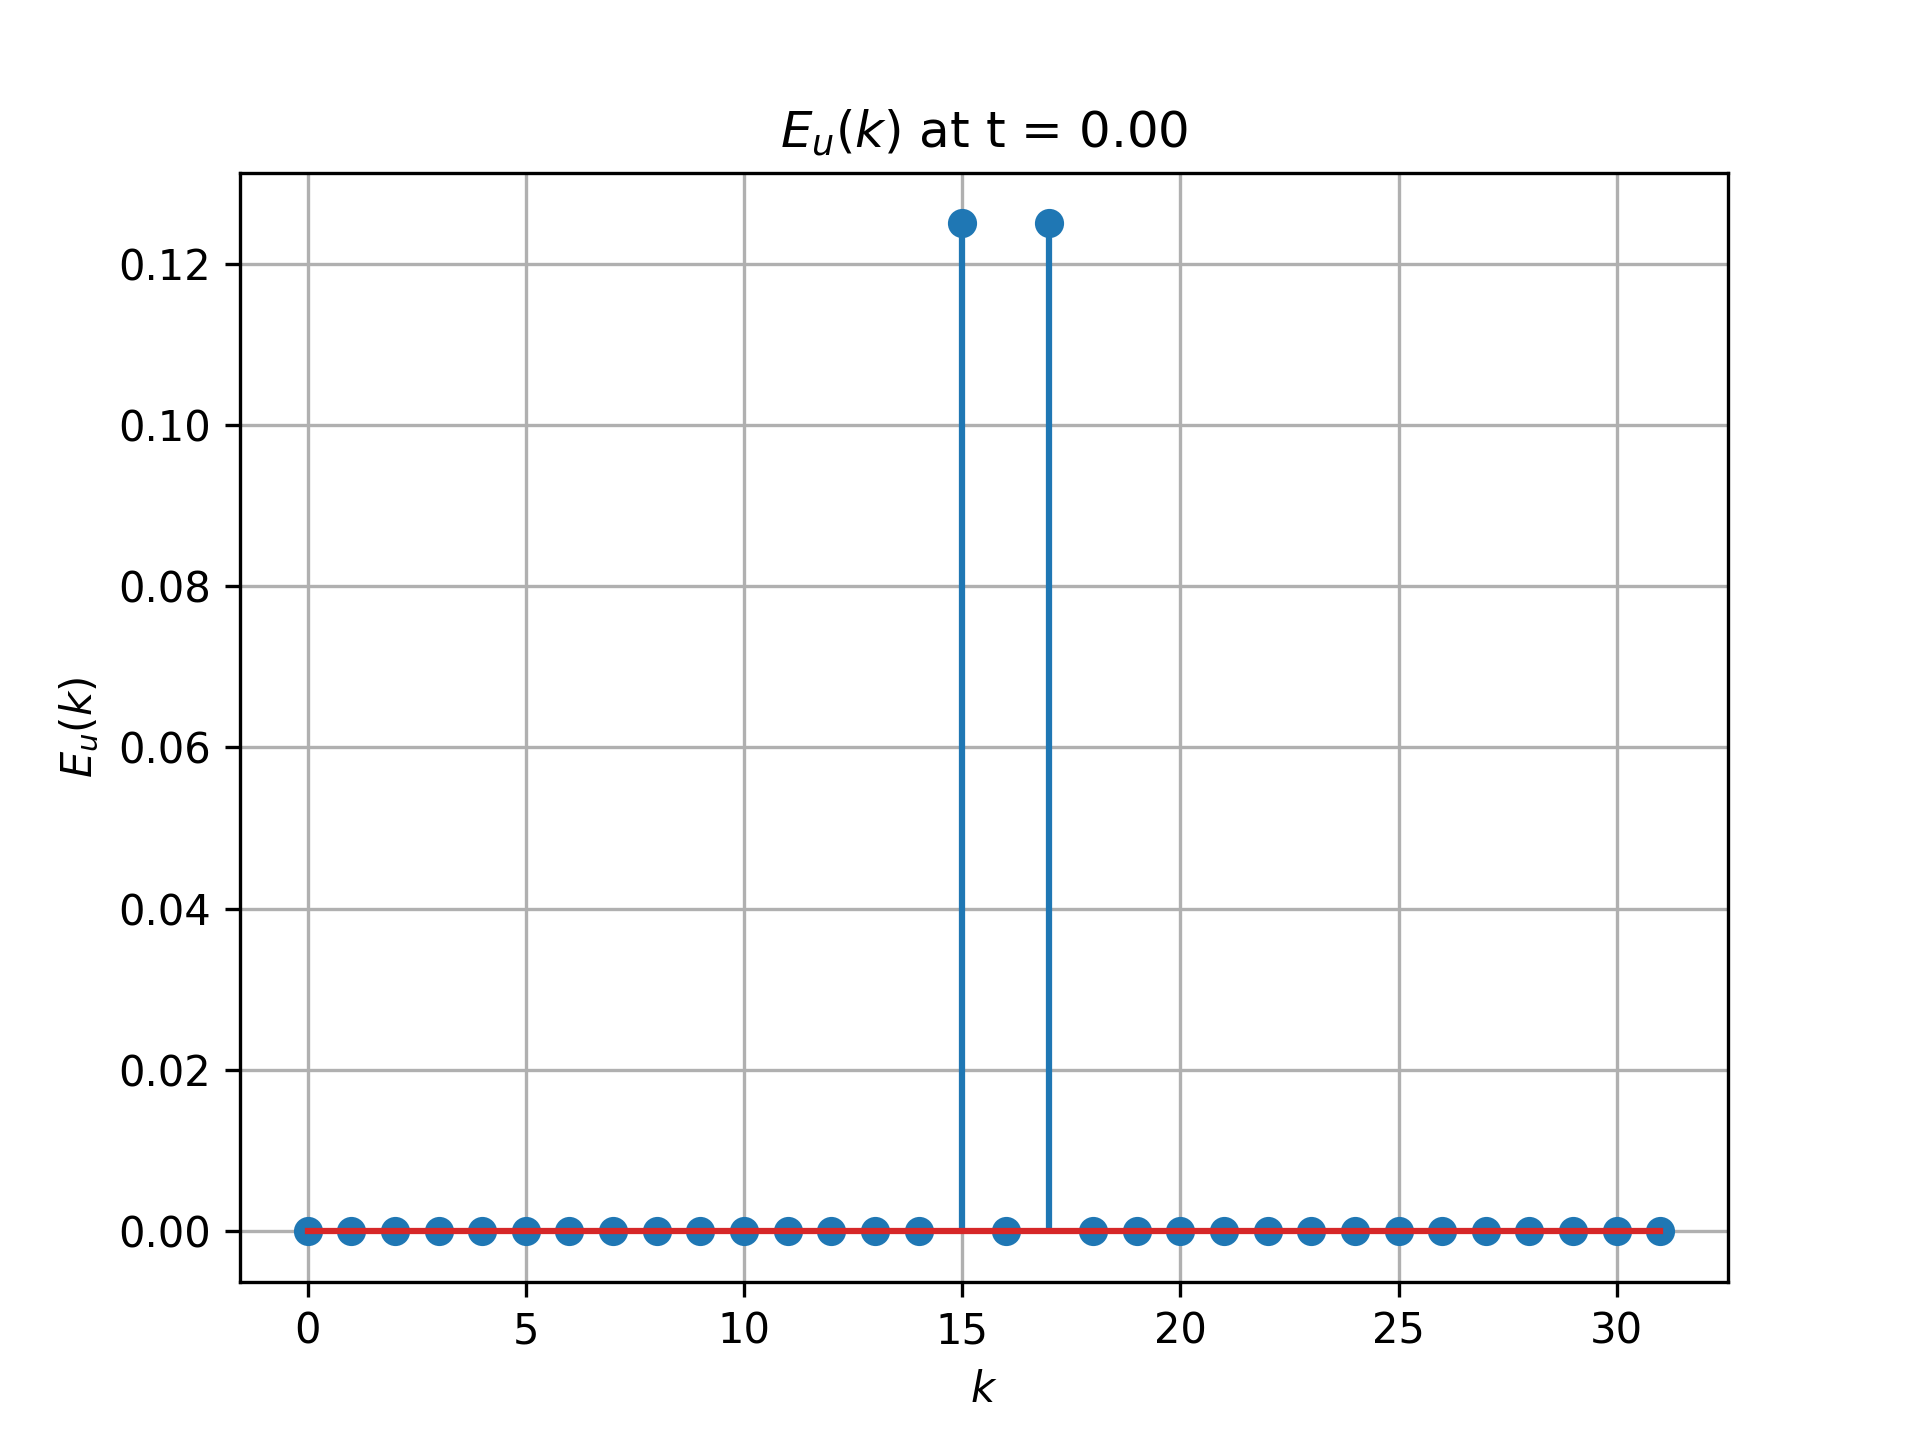
\includegraphics[width=6cm]{Code-Figures/espec-simple-1d/EK_spectrum.png}
      \caption{$1D$ $\vect{E}(\vect{k})$ field}
    \end{subfigure}
    \begin{subfigure}{7cm}
      \centering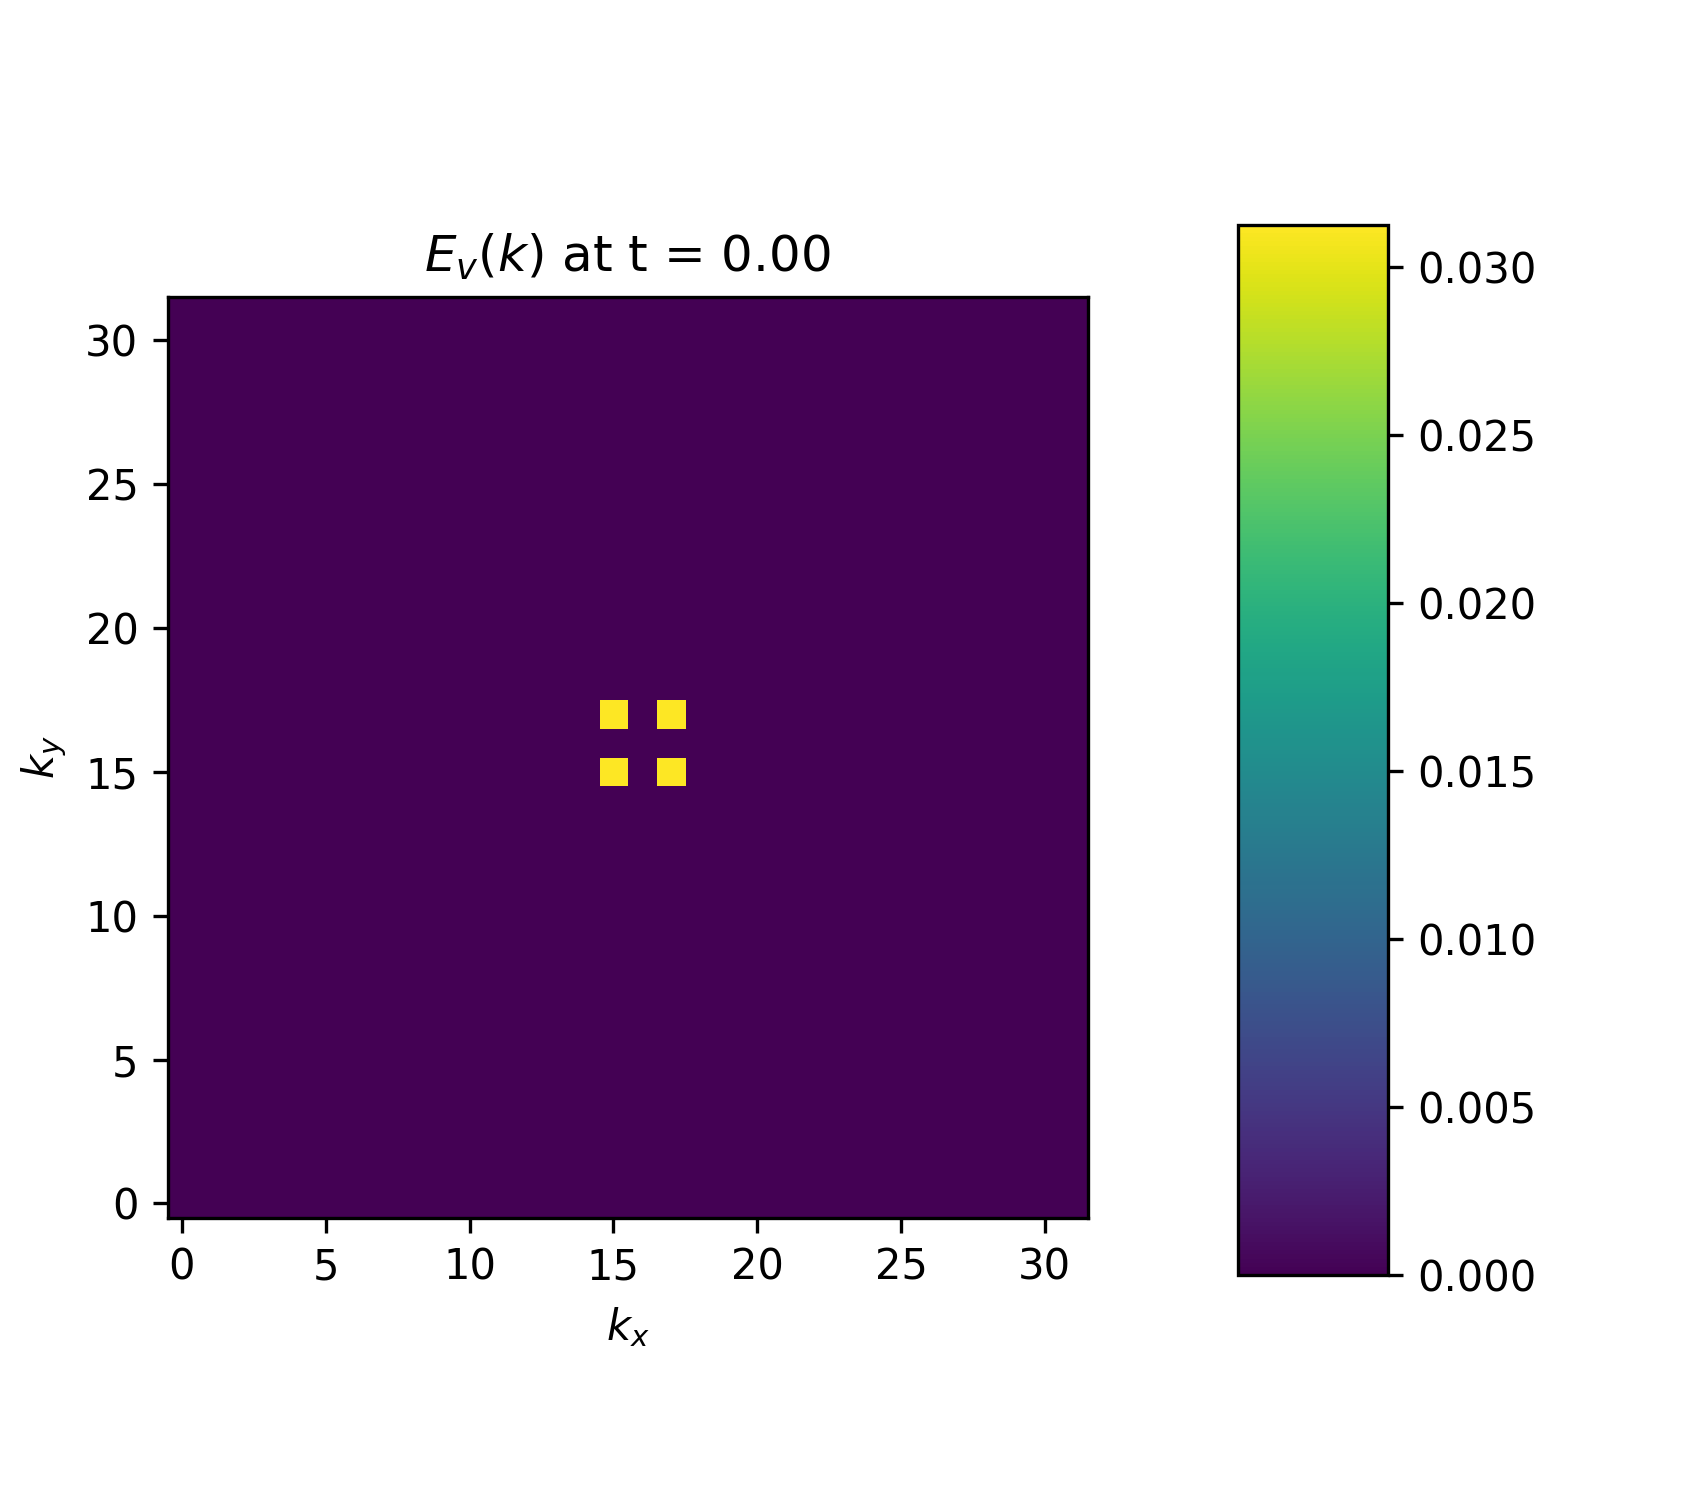
\includegraphics[width=6cm]{Code-Figures/espec-simple-2d/EK_spectrum.png}
      \caption{$2D$ $\vect{E}(\vect{k})$ field}
    \end{subfigure}
    \caption{The vector fields $\vect{E}(\vect{k})$ for $1D$ and $2D$ case, with decay rate $\gamma=0$, and $N=1$.}
    \label{fig:espec-vector-fields-N1}
\end{figure}

\begin{figure}[htbp!]
    \begin{subfigure}{7cm}
      \centering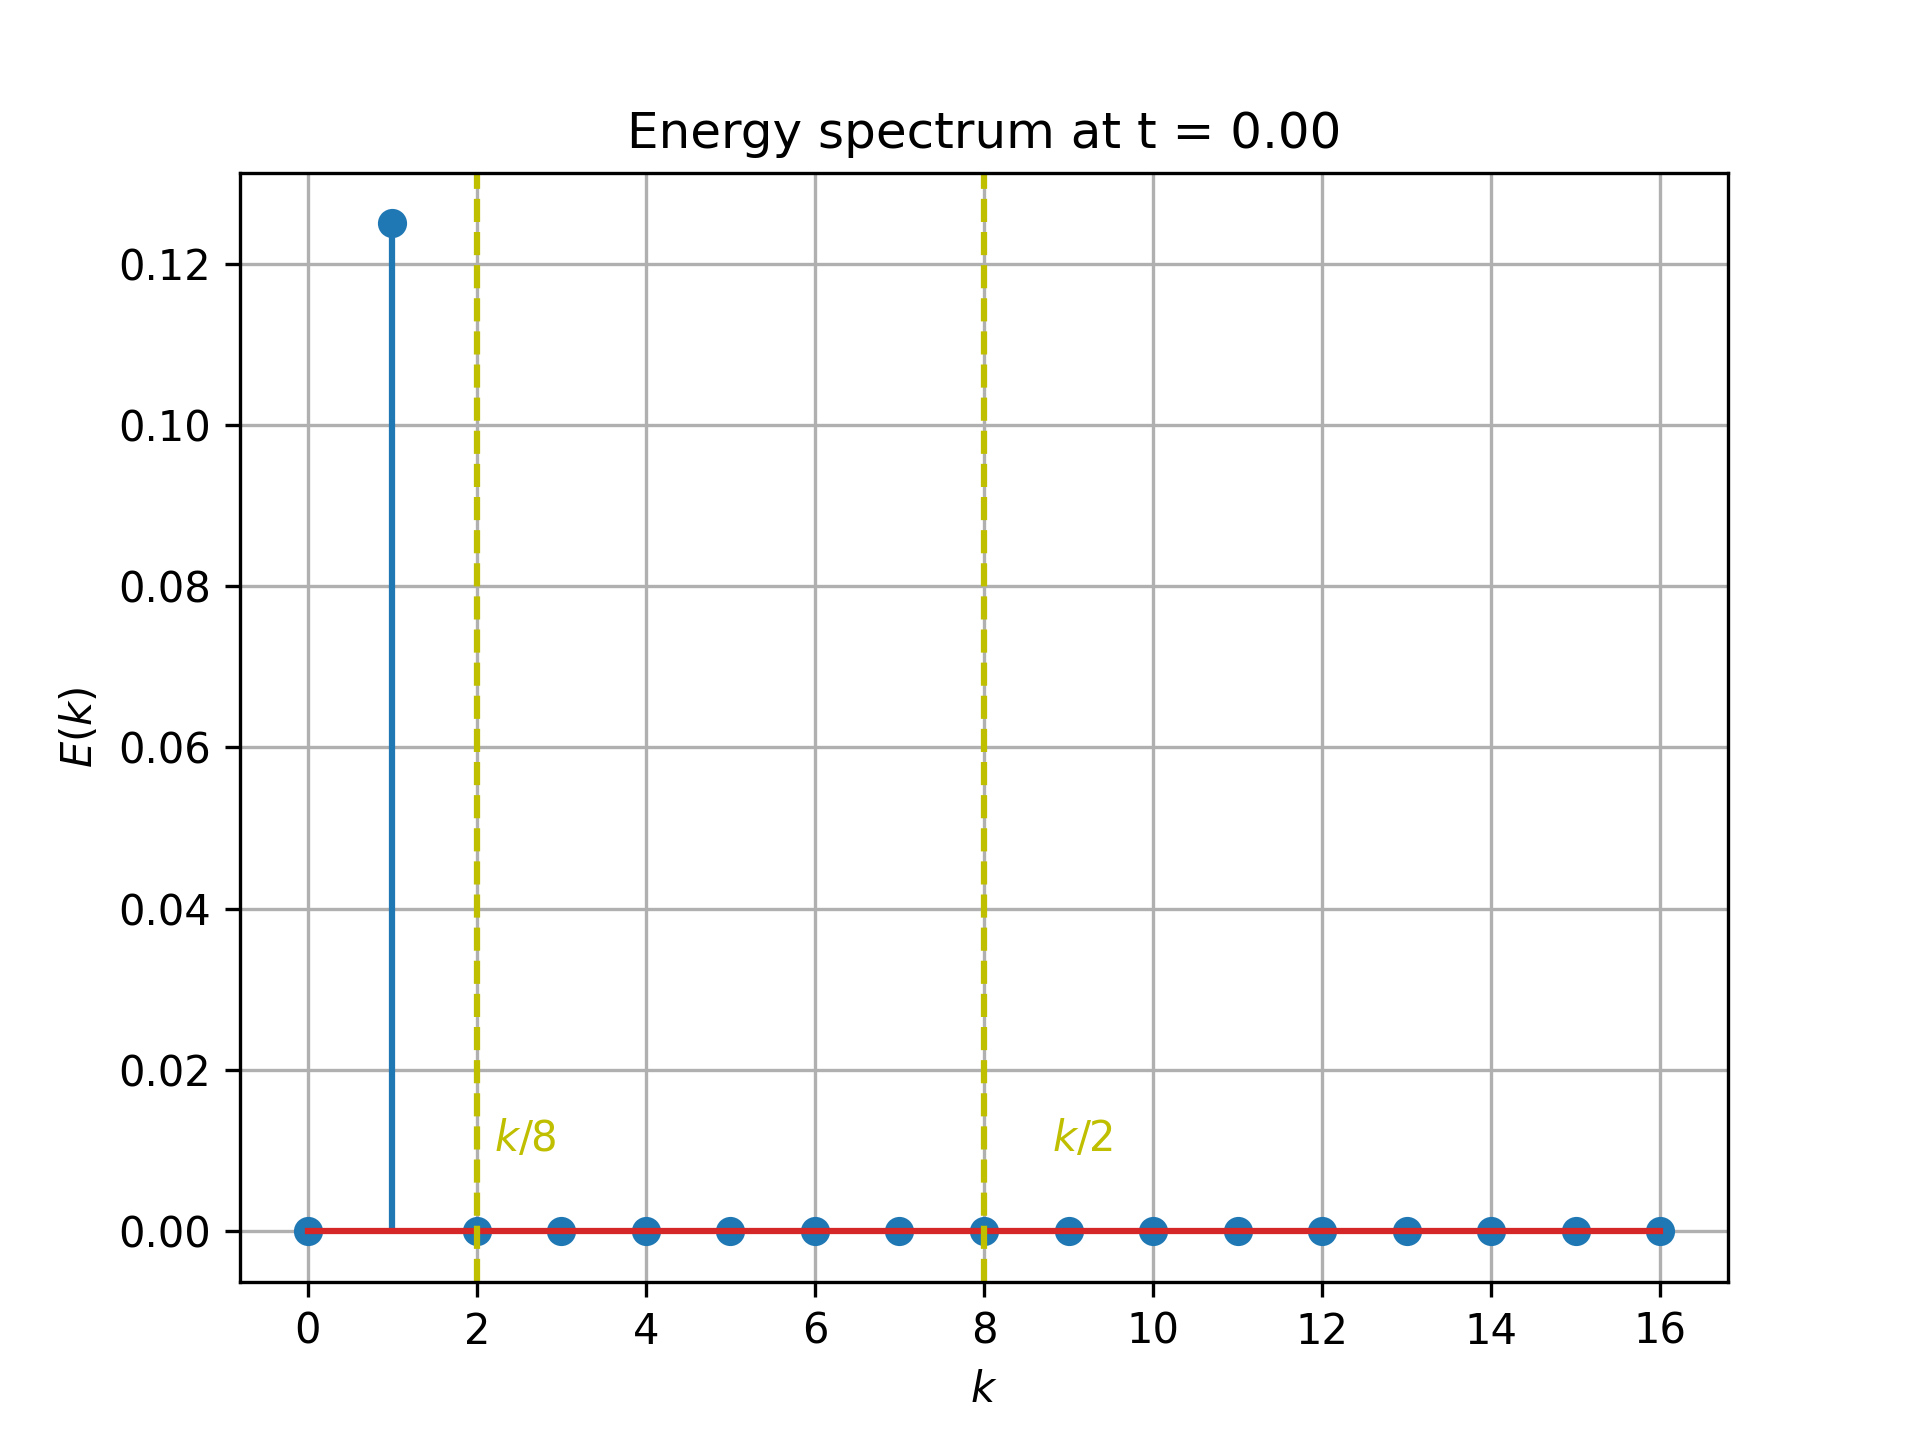
\includegraphics[width=6cm]{Code-Figures/espec-simple-1d/energy_spectrum.png}
      \caption{$1D$ $E(k)$ field}
    \end{subfigure}
    \begin{subfigure}{7cm}
      \centering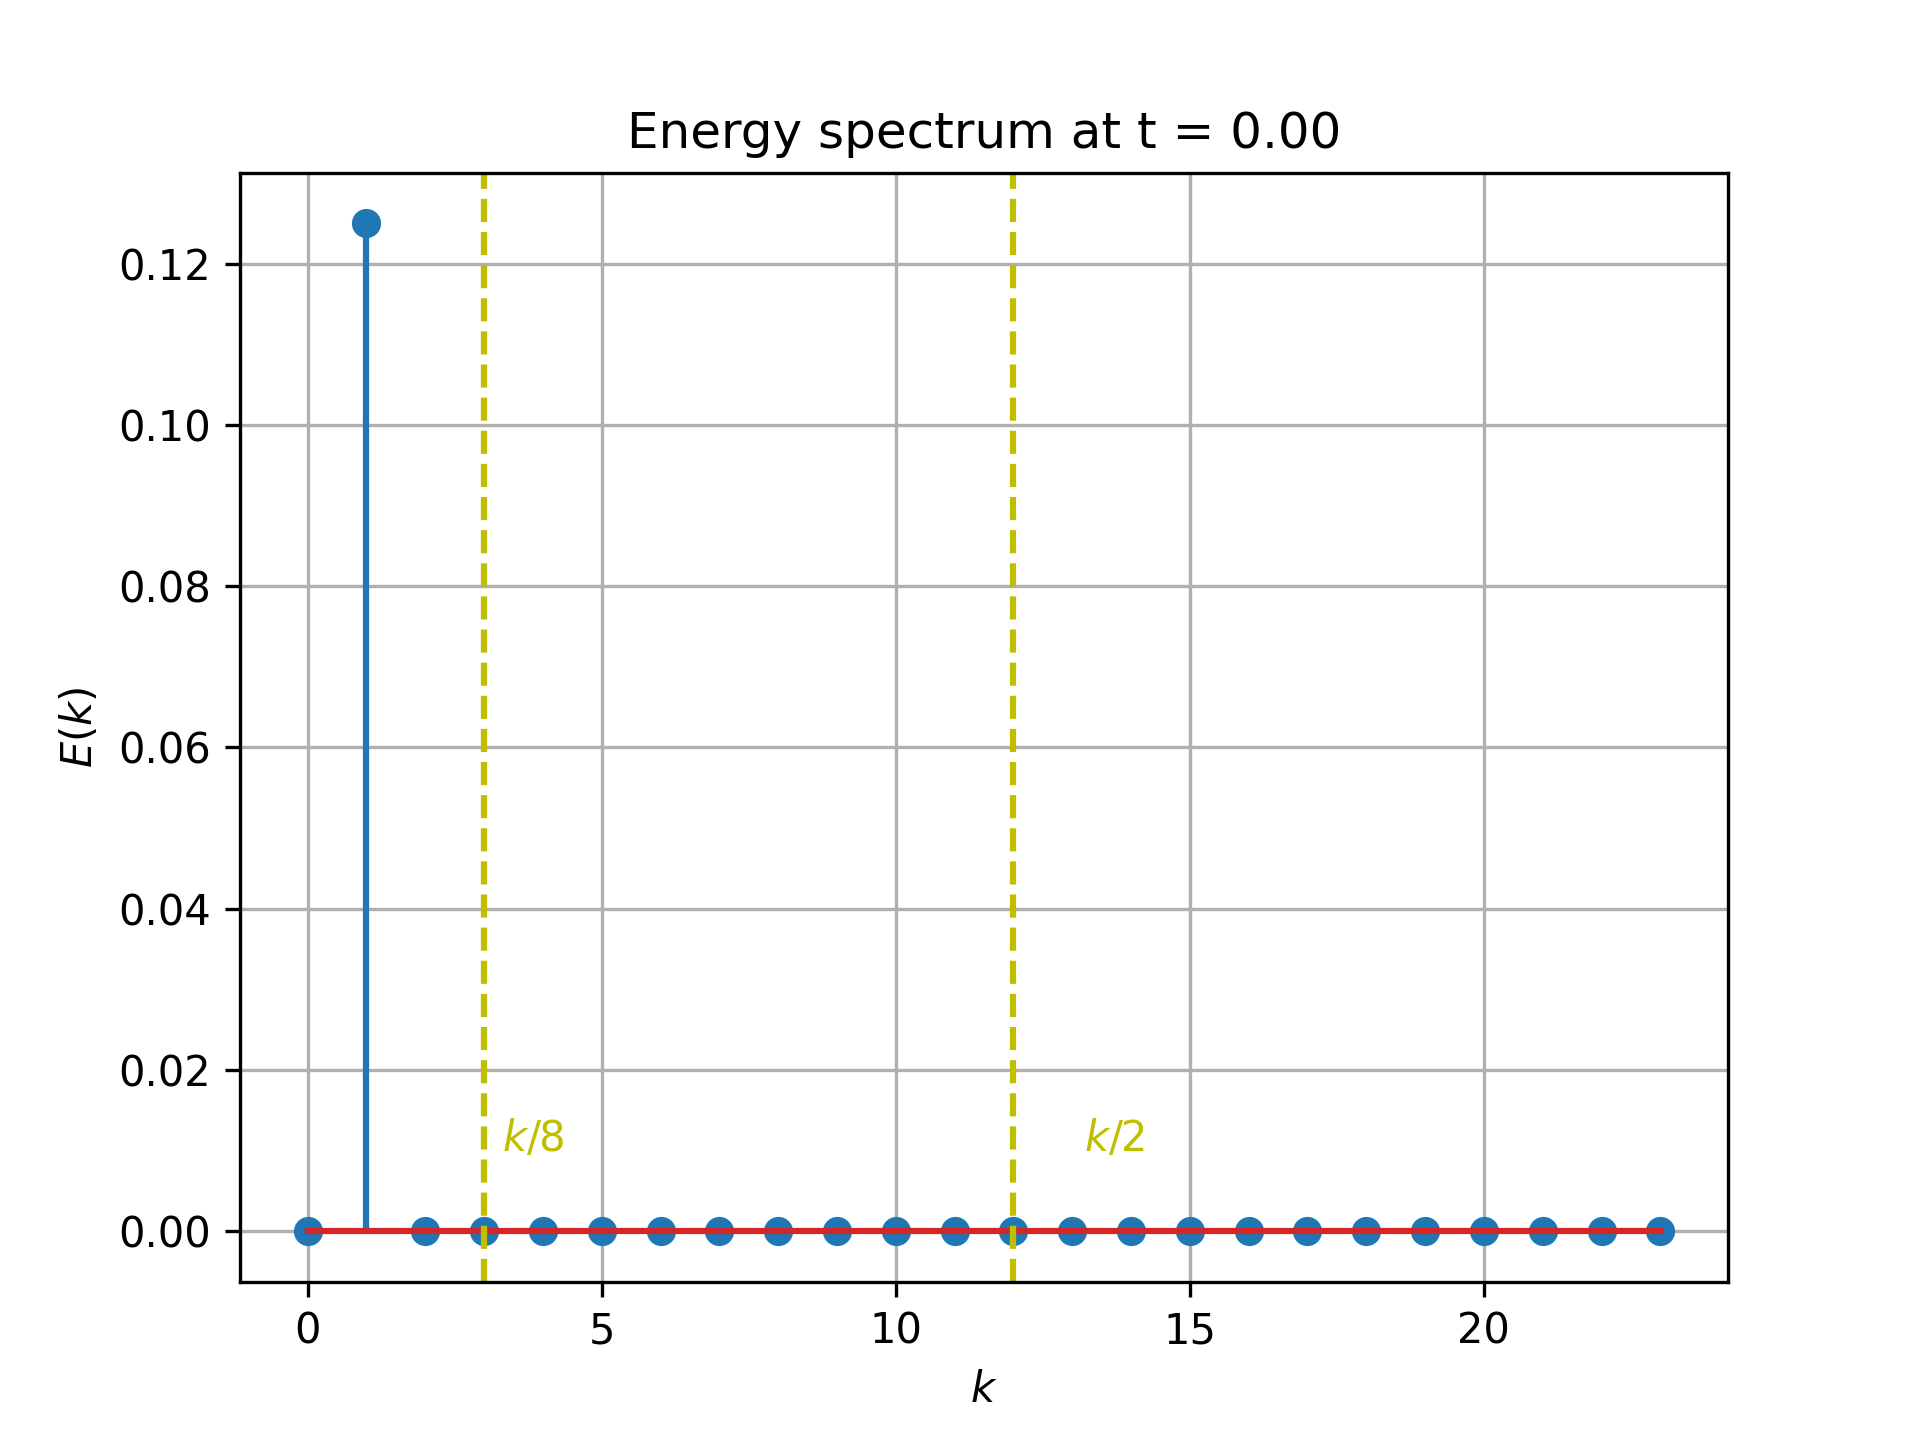
\includegraphics[width=6cm]{Code-Figures/espec-simple-2d/energy_spectrum.png}
      \caption{$2D$ $E(k)$ field}
    \end{subfigure}
    \begin{subfigure}{7cm}
        \centering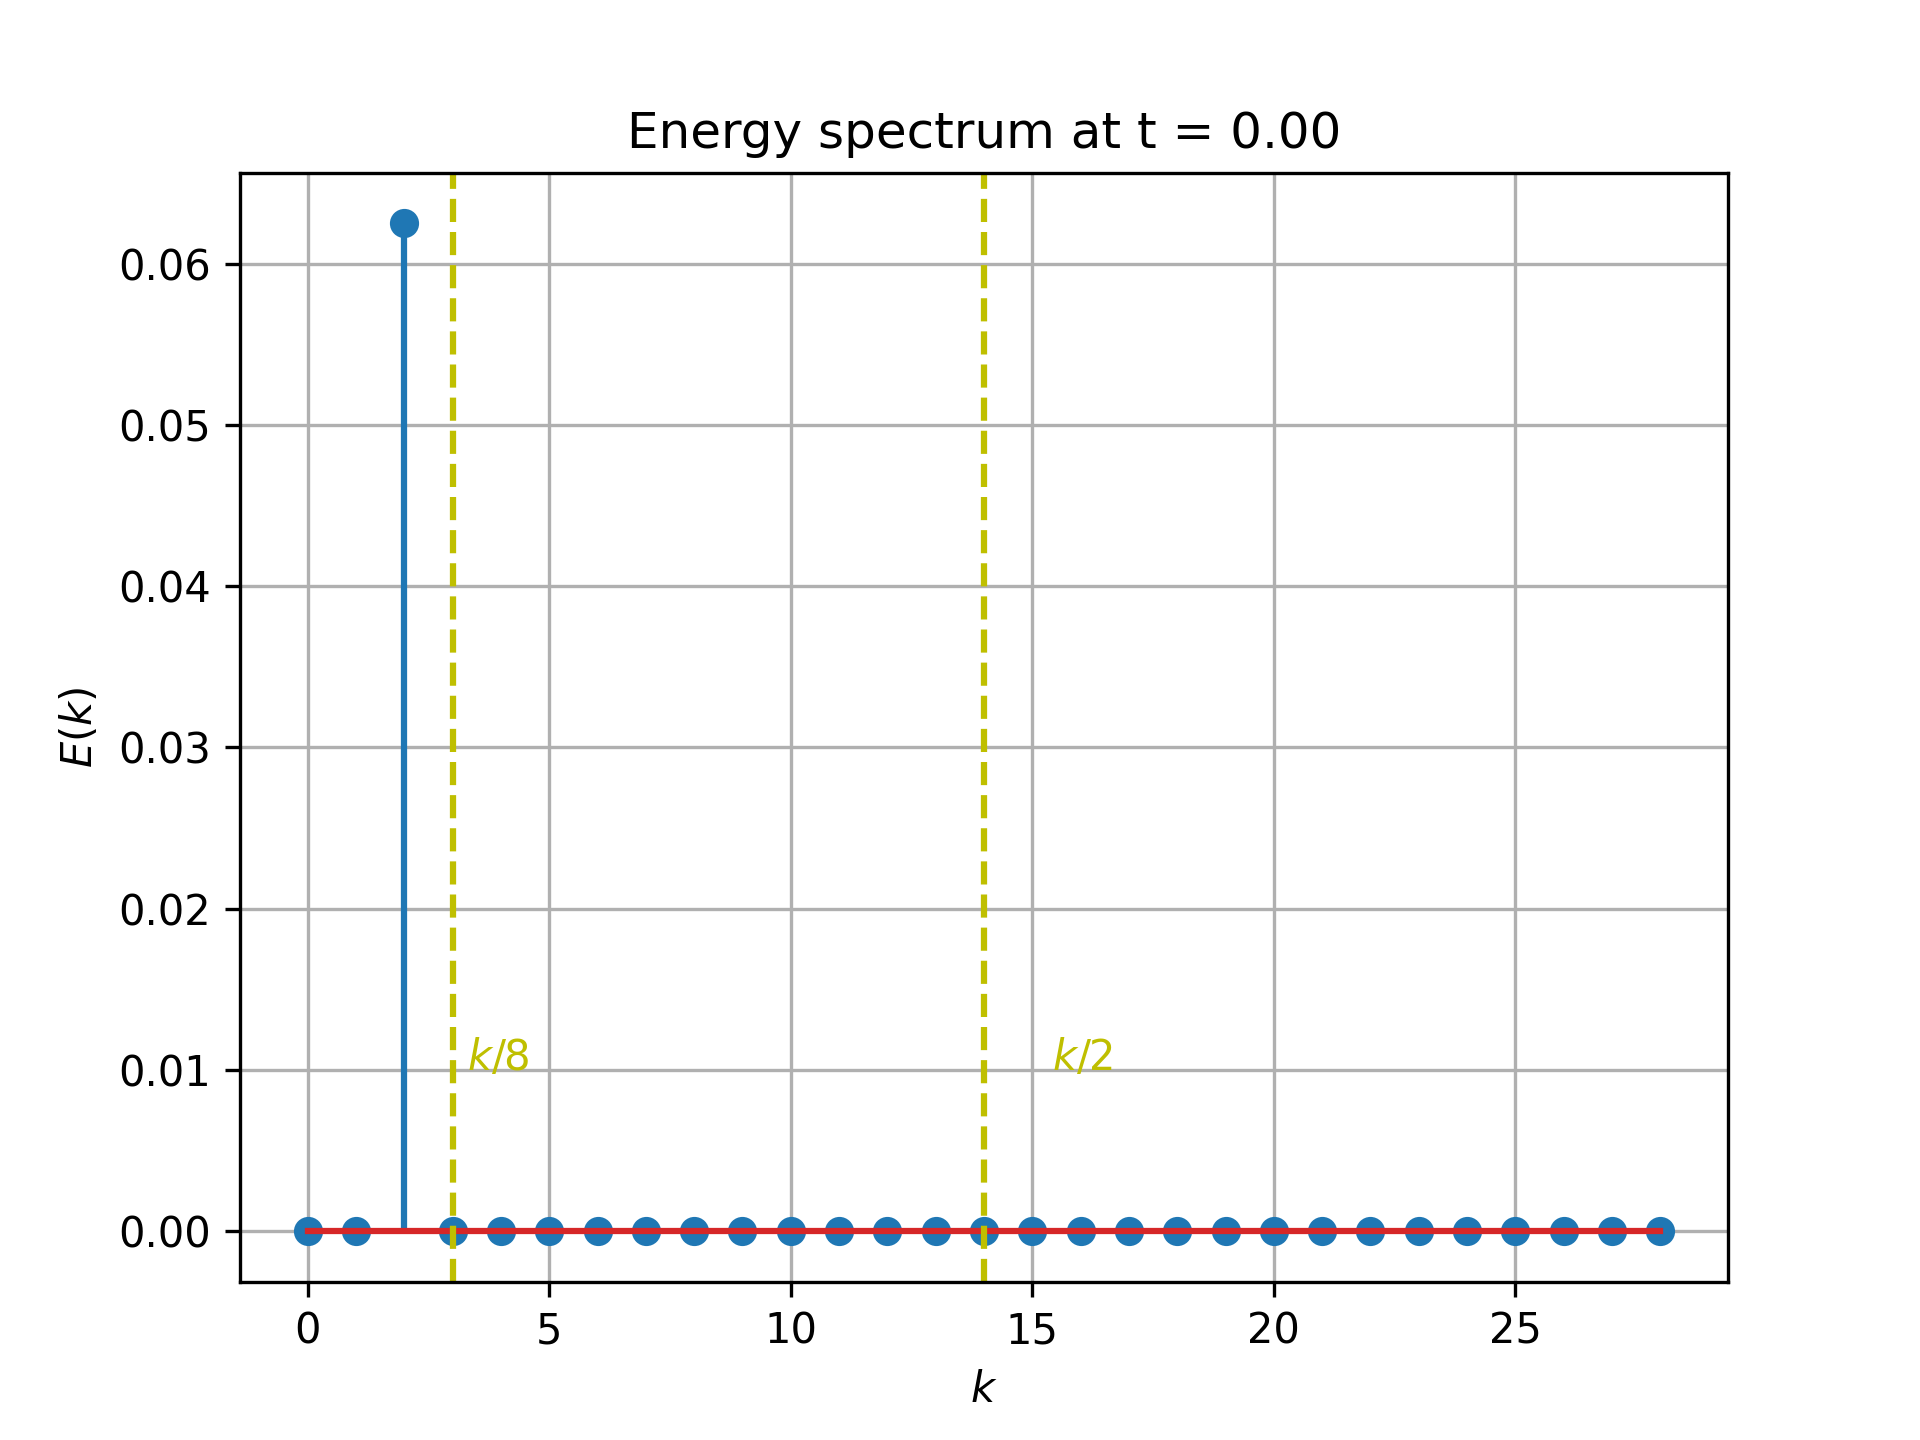
\includegraphics[width=6cm]{Code-Figures/espec-simple-3d/energy_spectrum.png}
        \caption{$3D$ $E(k)$ field}
      \end{subfigure}
    \caption{The scalar fields $E(k)$ for $1D$, $2D$, and $3D$ case, with decay rate $\gamma=0$, and $N=1$.}
    \label{fig:espec-scalar-fields-N1}
\end{figure}

Subsequently, the test cases were reconsidered to test the correctness when multiple modes are involved, with $\gamma=1$ and $N$ equal to half the number of particles along one axis of the problem.

The vector energy spectral fields are shown in \figref{fig:espec-vector-fields-gamma1}. Here, it can be observed that in both the $1D$ and $2D$ case, the energy spectrum peaks for $k=1$ and is non-zero up to $k=n_x/2$, indicating the nature of the velocity field, consisting of multiple modes. The amplitudes are also observed to have an exponential drop-off, as is expected, given the nature of the amplitude weighting.

This is made all the more apparent with the scalar energy spectral fields shown in \figref{fig:espec-scalar-fields-gamma1}. The log-log plots here allow for the exponential drop-off to be observed more clearly, by fitting a straight line to the log-log plot between wavenumbers $k \in [1, n_x/4]$. The gree-dashed lines, which represent the scalar energy spectrum computed for the original velocity field (which is uniform and rectangular) without interpolation, represent the `best'-case scenario, where the energy spectrum is computed without any loss of information in the velocity field, and the source of noise can be solely attributed to numerical errors from the discrete Fourier transform. The scalar energy spectrum computed from the interpolated velocity is plotted in blue.

It is observed that the energy spectrum computed without interpolation is indeed the `best'-case scenario since it much more closely follows the exact trend. However, with the computed energy spectrum from the interpolated velocity field, the trend is still observed to be followed, but only up to the $k/8$ wavenumber, beyond which the trend is lost, and the computed energy spectrum is observed to be much lower than the green-dashed line, with the difference increasing with the wavenumber.
This seems to indicate that the act of interpolation itself is introducing some amount of noise in the velocity field, which is reflected by the jagged nature of the blue line, and also seems to decrease the energy at lower scales, which is reflected by the blue line being consistently lower than the green-dashed line at lower wavenumbers. This allows for the conclusion that the interpolation scheme behaves as a low-pass filter, which is expected since the interpolation scheme is essentially a convolution of the velocity field with the kernel function, which is a low-pass filter.

Therefore, it was concluded that the $1D$ energy field, computed from the interpolated velocity field, typically will underestimate the energy at higher wavenumbers. Hence, the slope of the energy spectrum computed from the interpolated velocity field will be lower than the slope computed from the original velocity field, as reflected in \figref{fig:espec-scalar-fields-gamma1} as well.

\begin{figure}[htbp!]
    \begin{subfigure}{7cm}
      \centering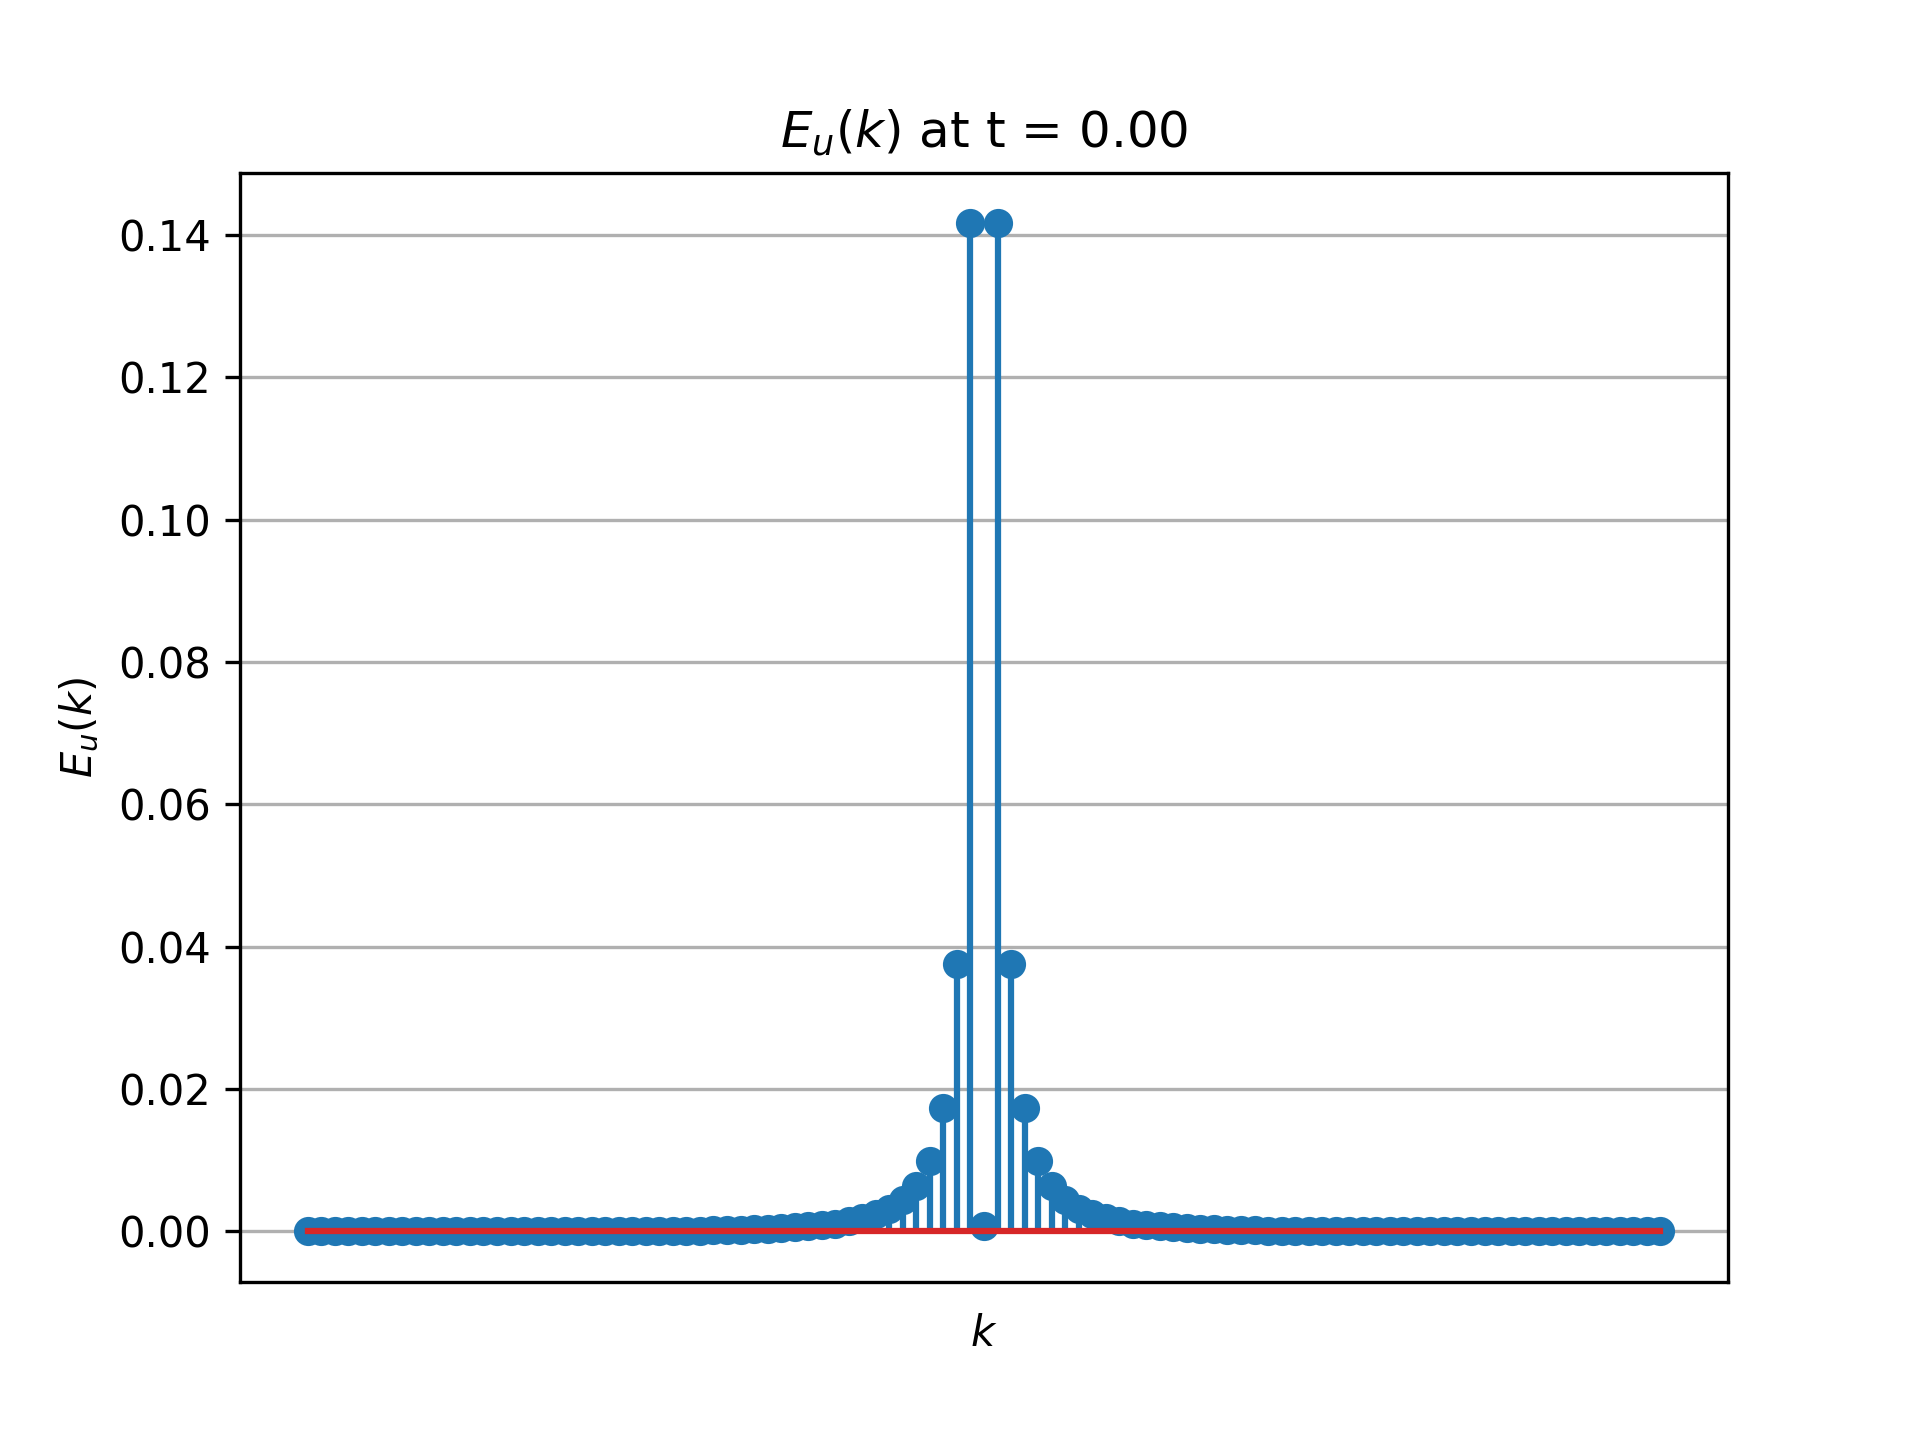
\includegraphics[width=6cm]{Code-Figures/sine-vel-prof-1d/EK_spectrum.png}
      \caption{$1D$ $\vect{E}(\vect{k})$ field}
    \end{subfigure}
    \begin{subfigure}{7cm}
      \centering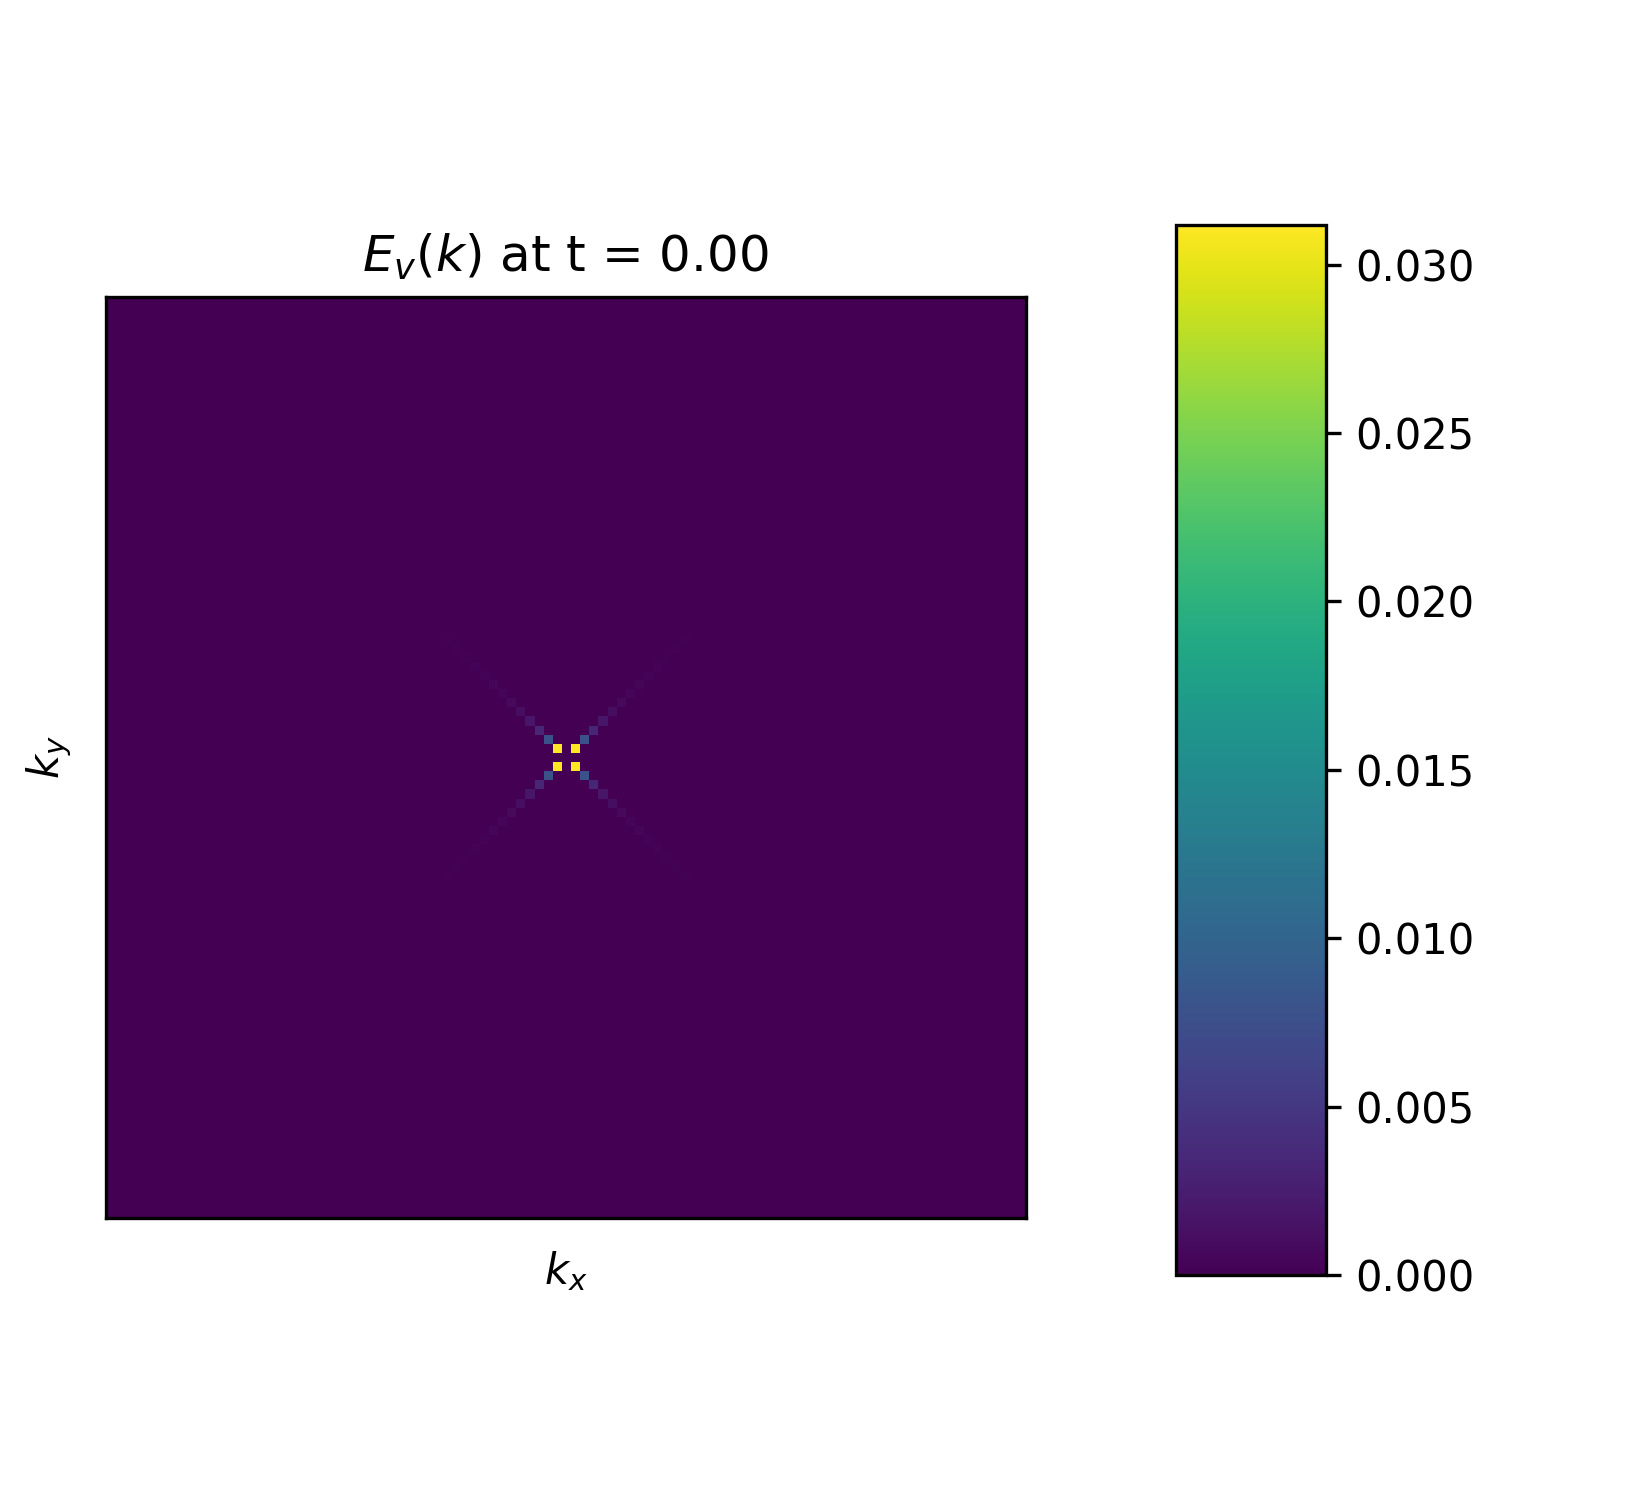
\includegraphics[width=6cm]{Code-Figures/sine-vel-prof-2d/EK_spectrum.png}
      \caption{$2D$ $\vect{E}(\vect{k})$ field}
    \end{subfigure}
    \caption{The vector fields $\vect{E}(\vect{k})$ for $1D$ and $2D$ case, with decay rate $\gamma=1$, and $N=n_x/2$.}
    \label{fig:espec-vector-fields-gamma1}
\end{figure}

\begin{figure}[htbp!]
    \begin{subfigure}{7cm}
      \centering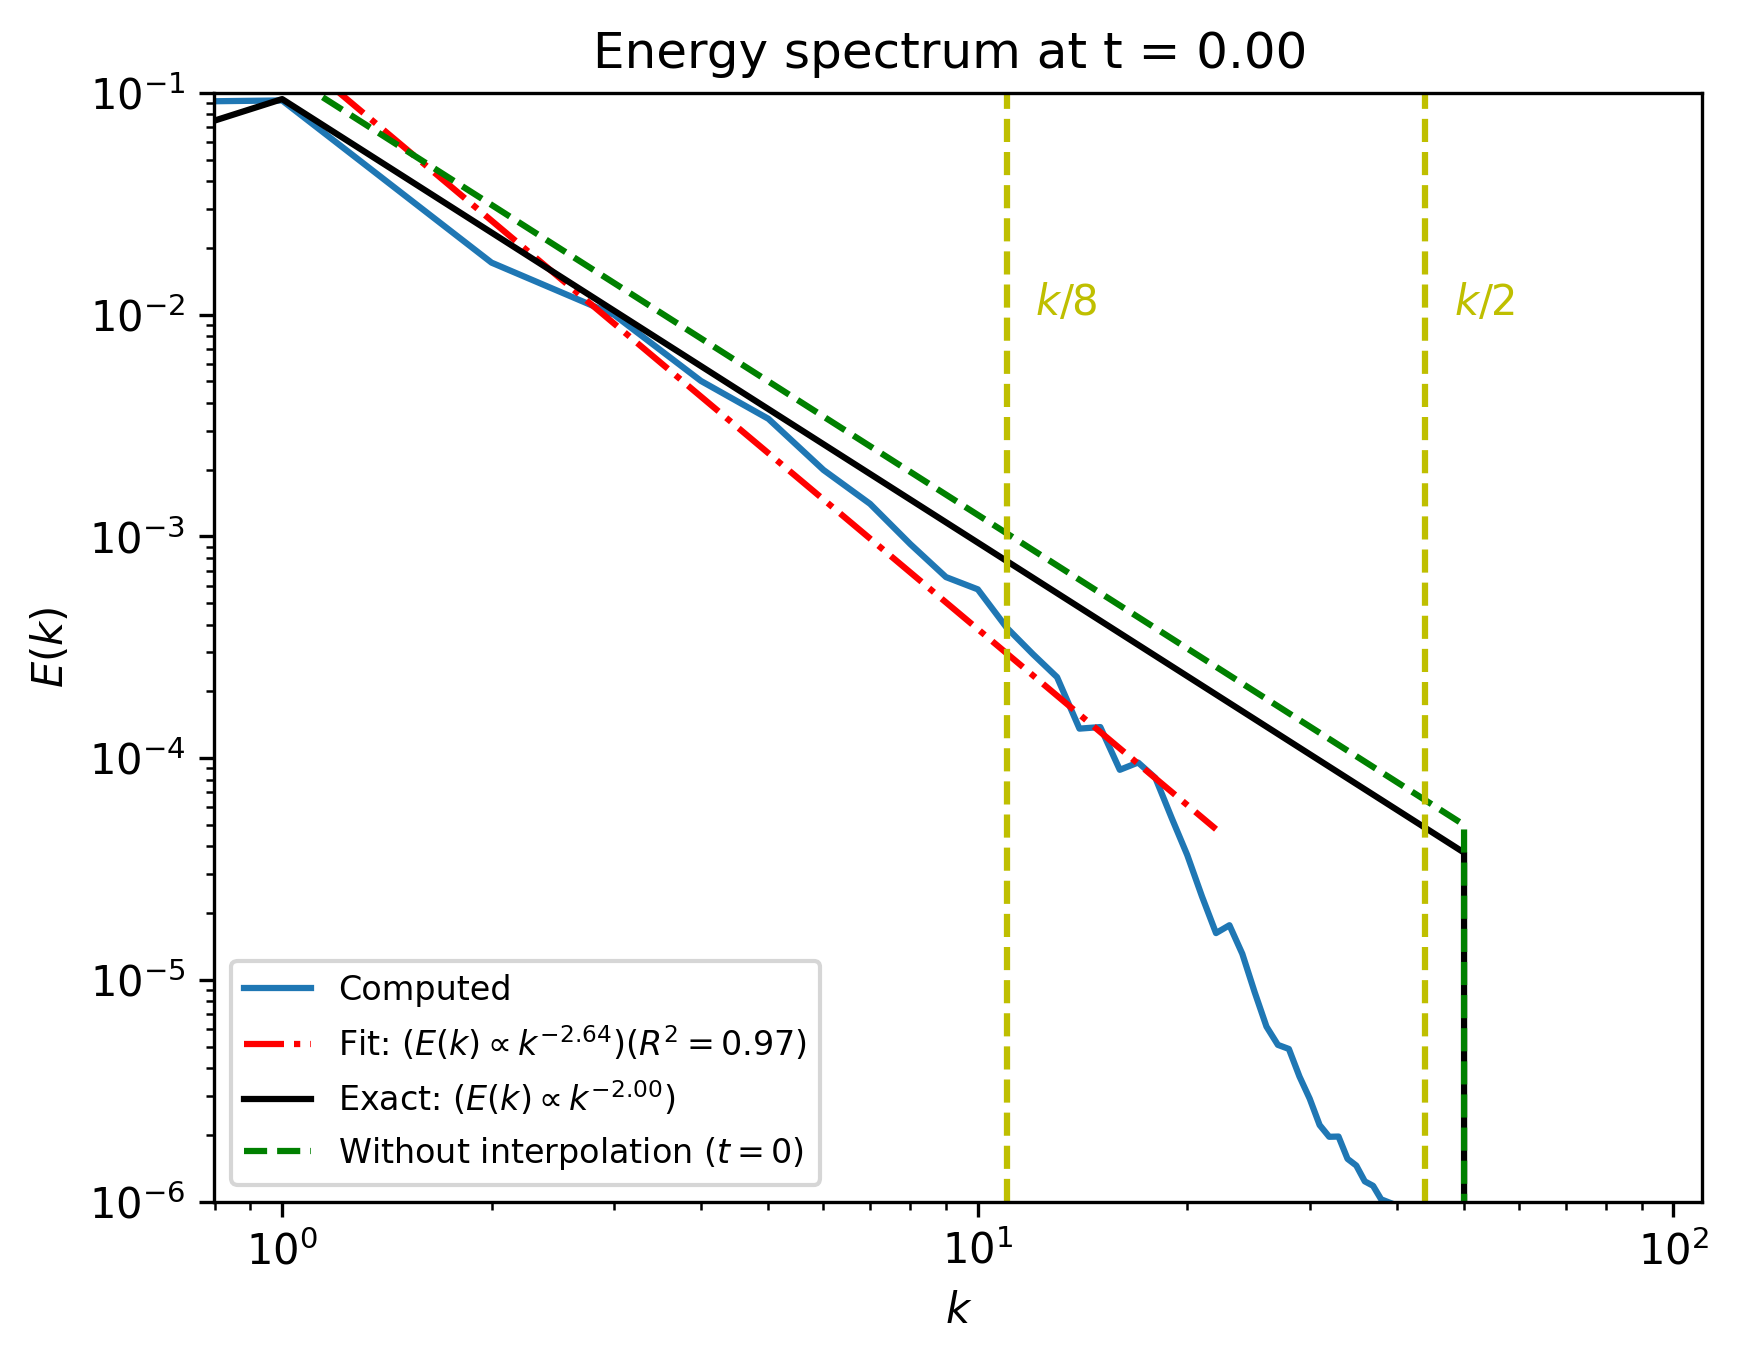
\includegraphics[width=6cm]{Code-Figures/sine-vel-prof-1d/ek_00000_loglog.png}
      \caption{$1D$ $E(k)$ field}
    \end{subfigure}
    \begin{subfigure}{7cm}
      \centering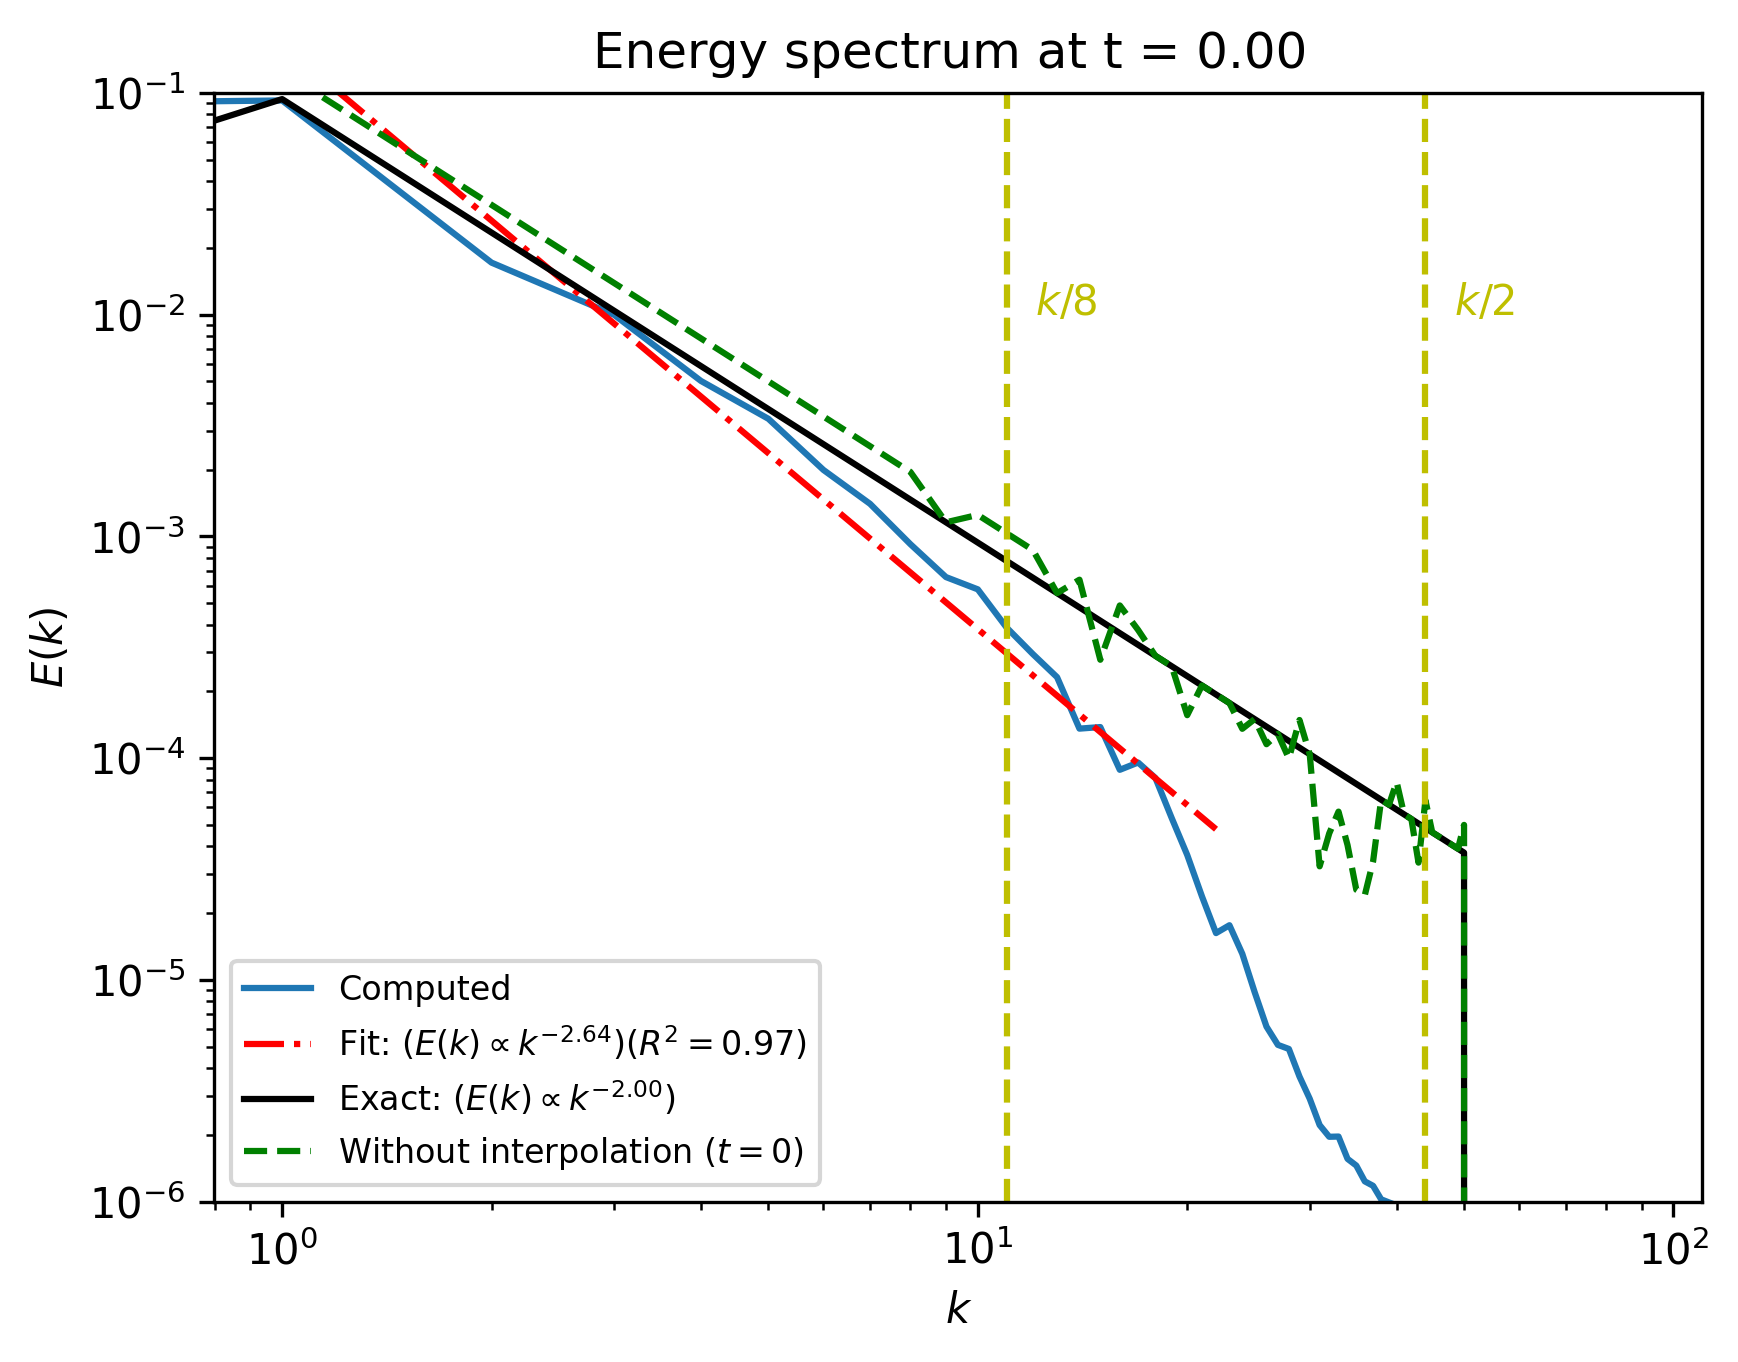
\includegraphics[width=6cm]{Code-Figures/sine-vel-prof-2d/ek_00000_loglog.png}
      \caption{$2D$ $E(k)$ field}
    \end{subfigure}
    \begin{subfigure}{7cm}
        \centering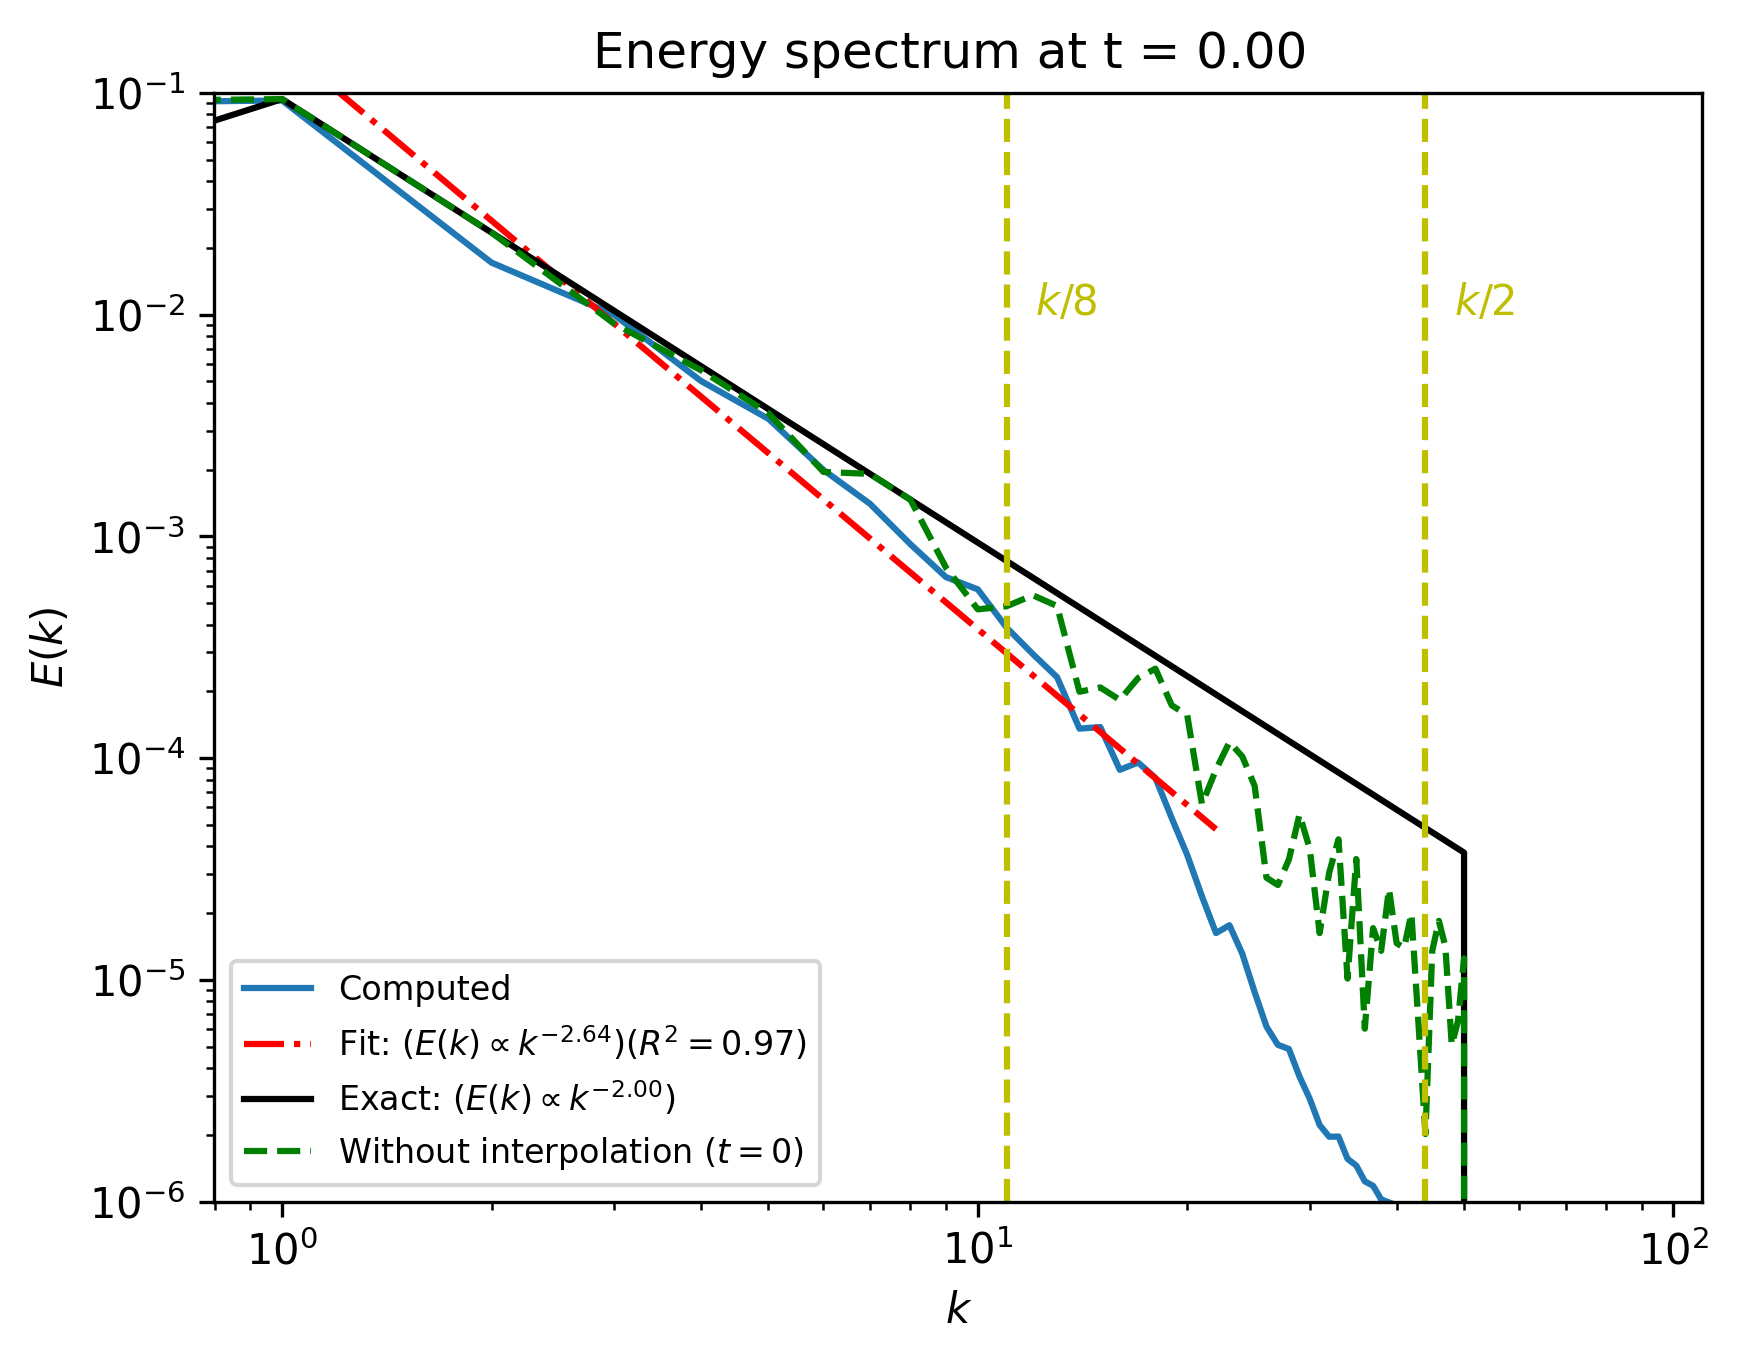
\includegraphics[width=6cm]{Code-Figures/sine-vel-prof-3d/ek_00000_loglog.png}
        \caption{$3D$ $E(k)$ field}
      \end{subfigure}
    \caption{The scalar fields $E(k)$ for $1D$, $2D$, and $3D$ case, with decay rate $\gamma=1$, and $N=n_x/2$.}
    \label{fig:espec-scalar-fields-gamma1}
\end{figure}

The same set of test cases, with $\gamma=1$ and $N=n_x/2$, are considered to identify the effect of various interpolation schemes, kernels, perturbation, and resolutions on the computed energy spectrum.

In order to measure the effect of the perturbation in the particle spacing on the computed energy spectrum, once a rectangular grid of uniform particles is defined, its coordinates are perturbed by a uniform random number $\delta \hat{x} \in [0, 1)$, scaled by a perturbation amplitude. The perturbed grid is then initialised with the corresponding velocity profile, and the energy spectrum is computed for the perturbed grid. From the results shown in \figref{fig:espec-scalar-fields-per-ampl}, it can be observed that by increasing the perturbation amplitude, energy seems to be introduced at lower resolution scales, which is reflected by the increased energy at higher wavenumbers. This trend seems to hold for all dimensions.
Therefore, we can infer that the low-pass energy dissipation effect of the interpolation scheme will to an extent, be countered by the perturbation in the particle spacing (which is typically the case in a simulation since the particles become disturbed), which will introduce energy at lower resolution scales, and hence, the slope of the energy spectrum computed from the interpolated velocity field will be closer to the slope of the energy spectrum computed from the original velocity field. 

\begin{figure}[htbp!]
    \begin{subfigure}{7cm}
      \centering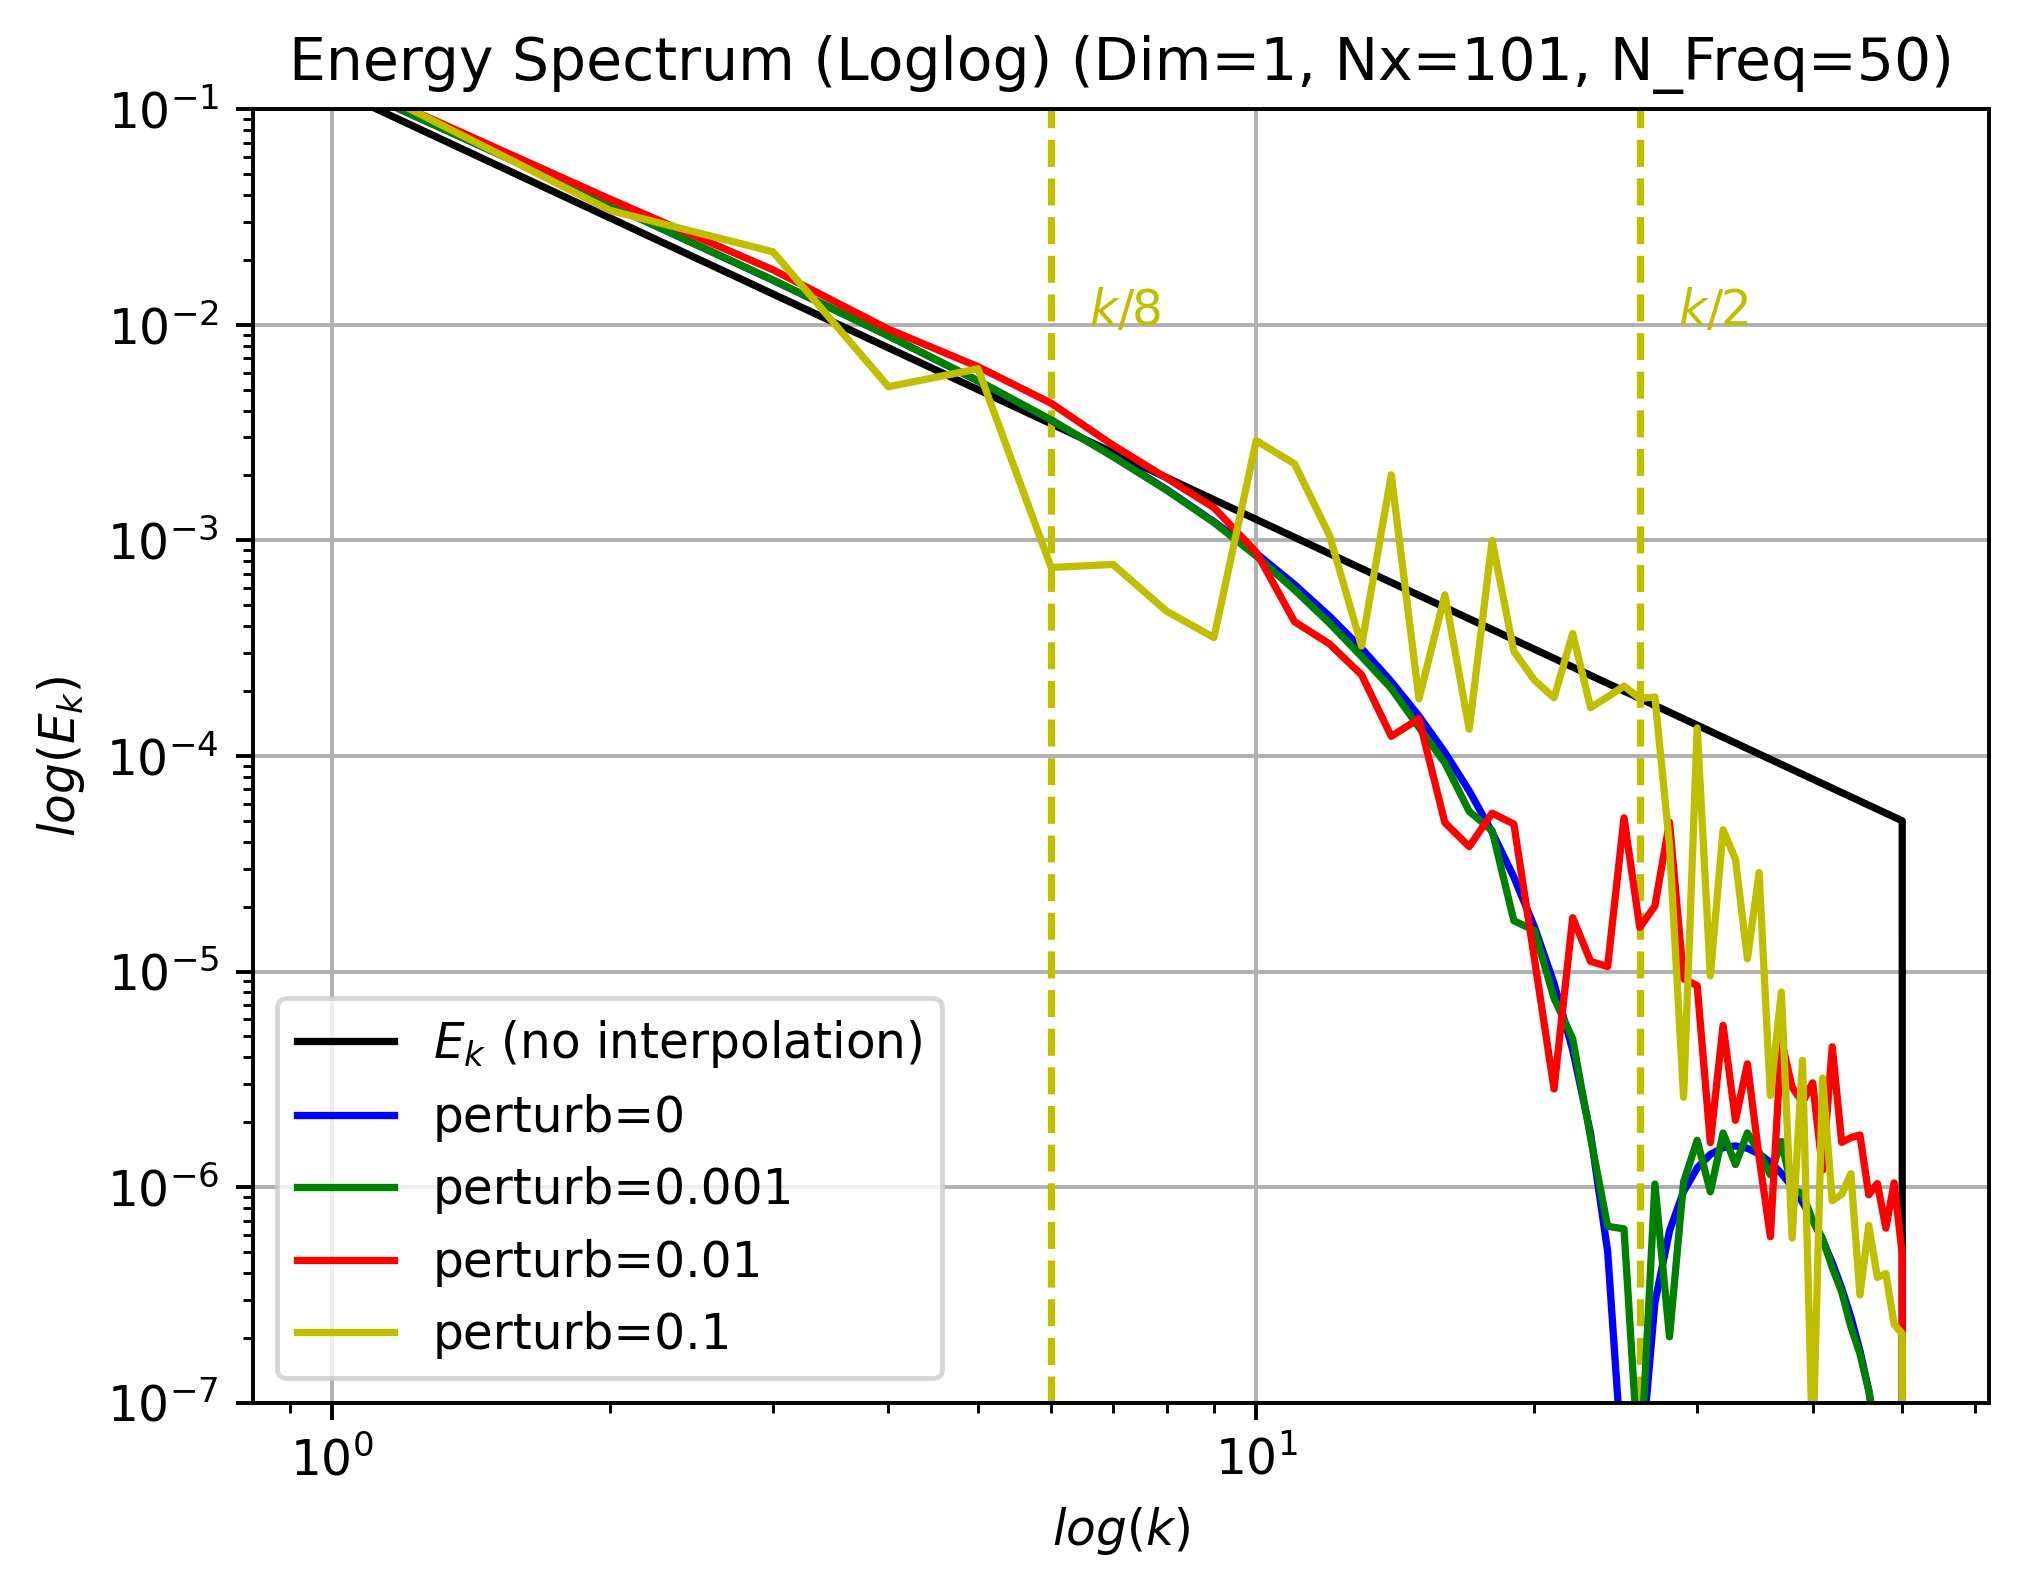
\includegraphics[width=6cm]{Code-Figures/sin-vel-prof-pertub/Energy Spectrum (Loglog) (Dim=1, Nx=101, N_Freq=50).png}
      \caption{$1D$ $E(k)$ field}
    \end{subfigure}
    \begin{subfigure}{7cm}
      \centering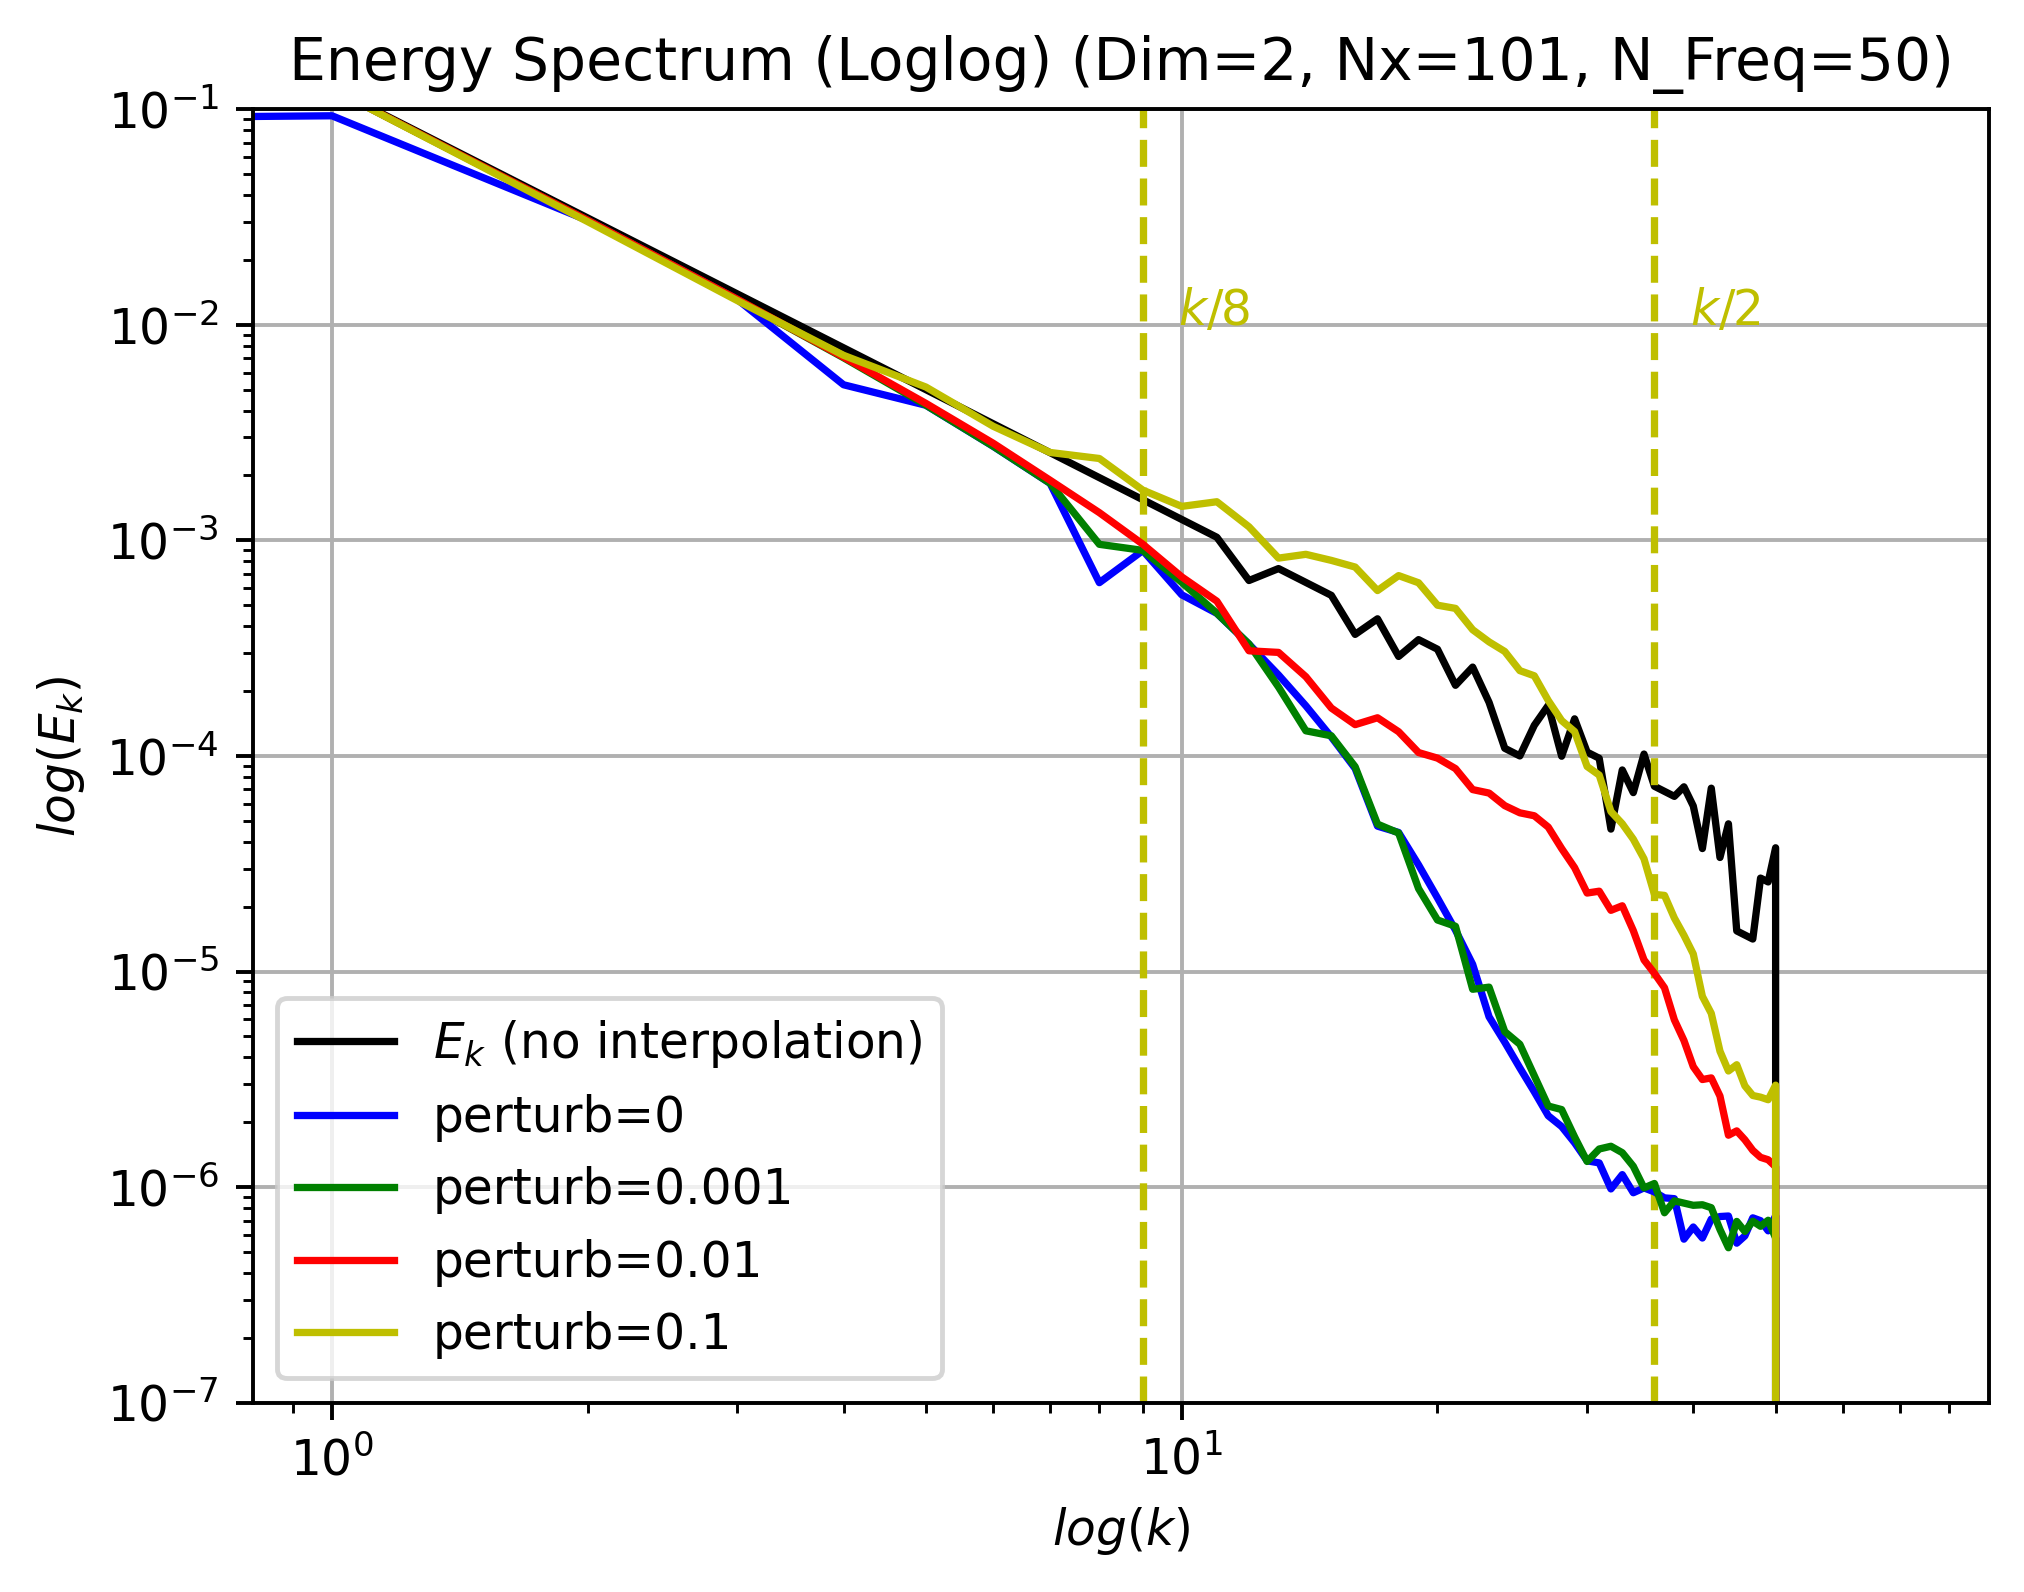
\includegraphics[width=6cm]{Code-Figures/sin-vel-prof-pertub/Energy Spectrum (Loglog) (Dim=2, Nx=101, N_Freq=50).png}
      \caption{$2D$ $E(k)$ field}
    \end{subfigure}
    \begin{subfigure}{7cm}
        \centering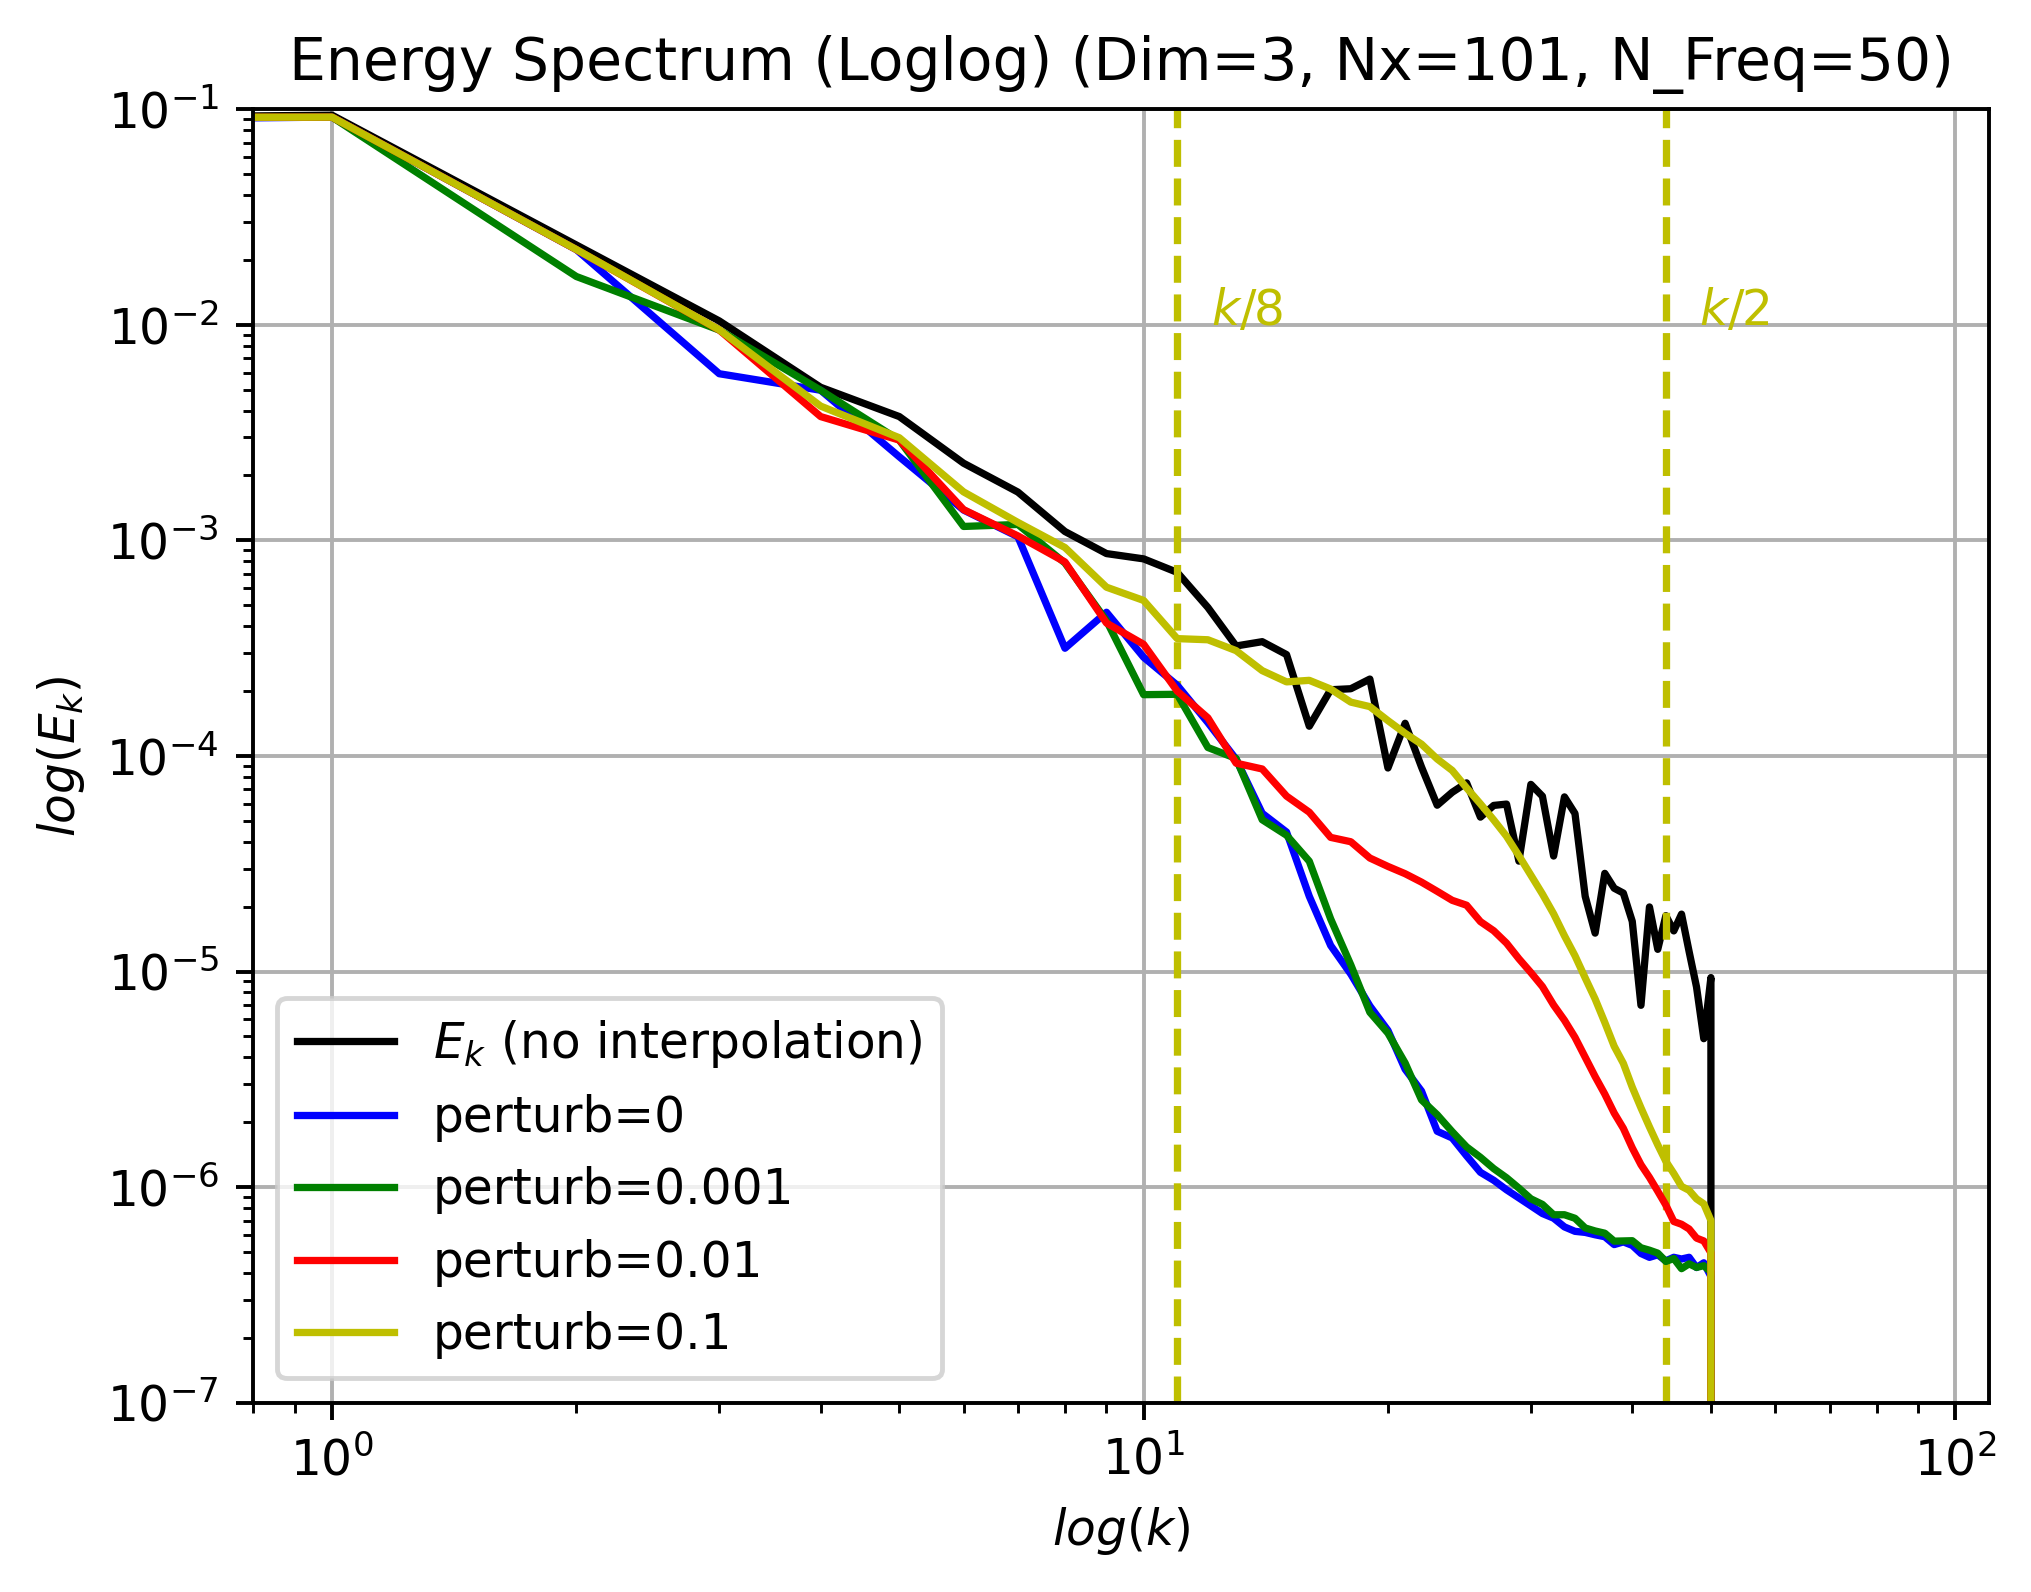
\includegraphics[width=6cm]{Code-Figures/sin-vel-prof-pertub/Energy Spectrum (Loglog) (Dim=3, Nx=101, N_Freq=50).png}
        \caption{$3D$ $E(k)$ field}
      \end{subfigure}
    \caption{The scalar fields $E(k)$ for $1D$, $2D$, and $3D$ case, for various perturbation amplitudes.}
    \label{fig:espec-scalar-fields-per-ampl}
\end{figure}

Then, in order to measure the effect of the interpolation scheme on the computed energy spectrum, the following interpolation schemes were considered:
\begin{itemize}
    \item \texttt{sph}:
    \begin{equation}
        \hat{\phi_i} = \sum_{ij} \frac{m_j}{\rho_j} \phi_j \DWIJ,
    \end{equation}
    
    \item \texttt{shepard}:
    \begin{equation}
        \hat{\phi_i} = \frac{\sum_{ij} \phi_j \WIJ}{\sum_{ij} \WIJ},
    \end{equation}

    \item \texttt{order1} \parencite{Liu2006}:
    \begin{equation}
      \tensor{A}_{4 \times 4} \vect{x}_{4 \times 1} = \vect{b}_{4 \times 1}
      \label{eq:interp-order1}
    \end{equation}
    where $\tensor{A}$ is the moment matrix, $\vect{b} = [\phi, \nabla \phi]^T$ is the interpolated property, and its gradient is calculated using basic SPH, and $\vect{x} = [\hat{\phi}, \nabla \hat{\phi}]^T$ is the unknown interpolated property and its gradient,

    \item \texttt{order1BL}: same as \Eqref{eq:interp-order1}, but with the $\DWIJ$ term corrected using the Bonet-Lok correction \parencite{bonet1999variational},

    \item \texttt{order1MC}: same as \Eqref{eq:interp-order1}, but with the $\DWIJ$ term corrected using the Mixed-Kernel correction \parencite{bonet1999variational},
\end{itemize}
where $\phi$ is the quantity to be interpolated, and $\hat{\phi}$ is the interpolated quantity.

From the results shown in \figref{fig:espec-scalar-fields-i-methods}, it can be observed that the \texttt{order1MC} interpolation scheme seems to introduce the least amount of energy at lower resolution scales, with the \texttt{sph} scheme introducing the most amount of energy at lower resolution scales. This trend seems to hold for all dimensions.
Therefore, because the \texttt{sph} interpolation scheme would appear to counter the loss in energy at lower resolution scales due to the act of interpolation, it is chosen as the default interpolation scheme for the computation of the energy spectrum.

\begin{figure}[htbp!]
	\begin{subfigure}{7cm}
		\centering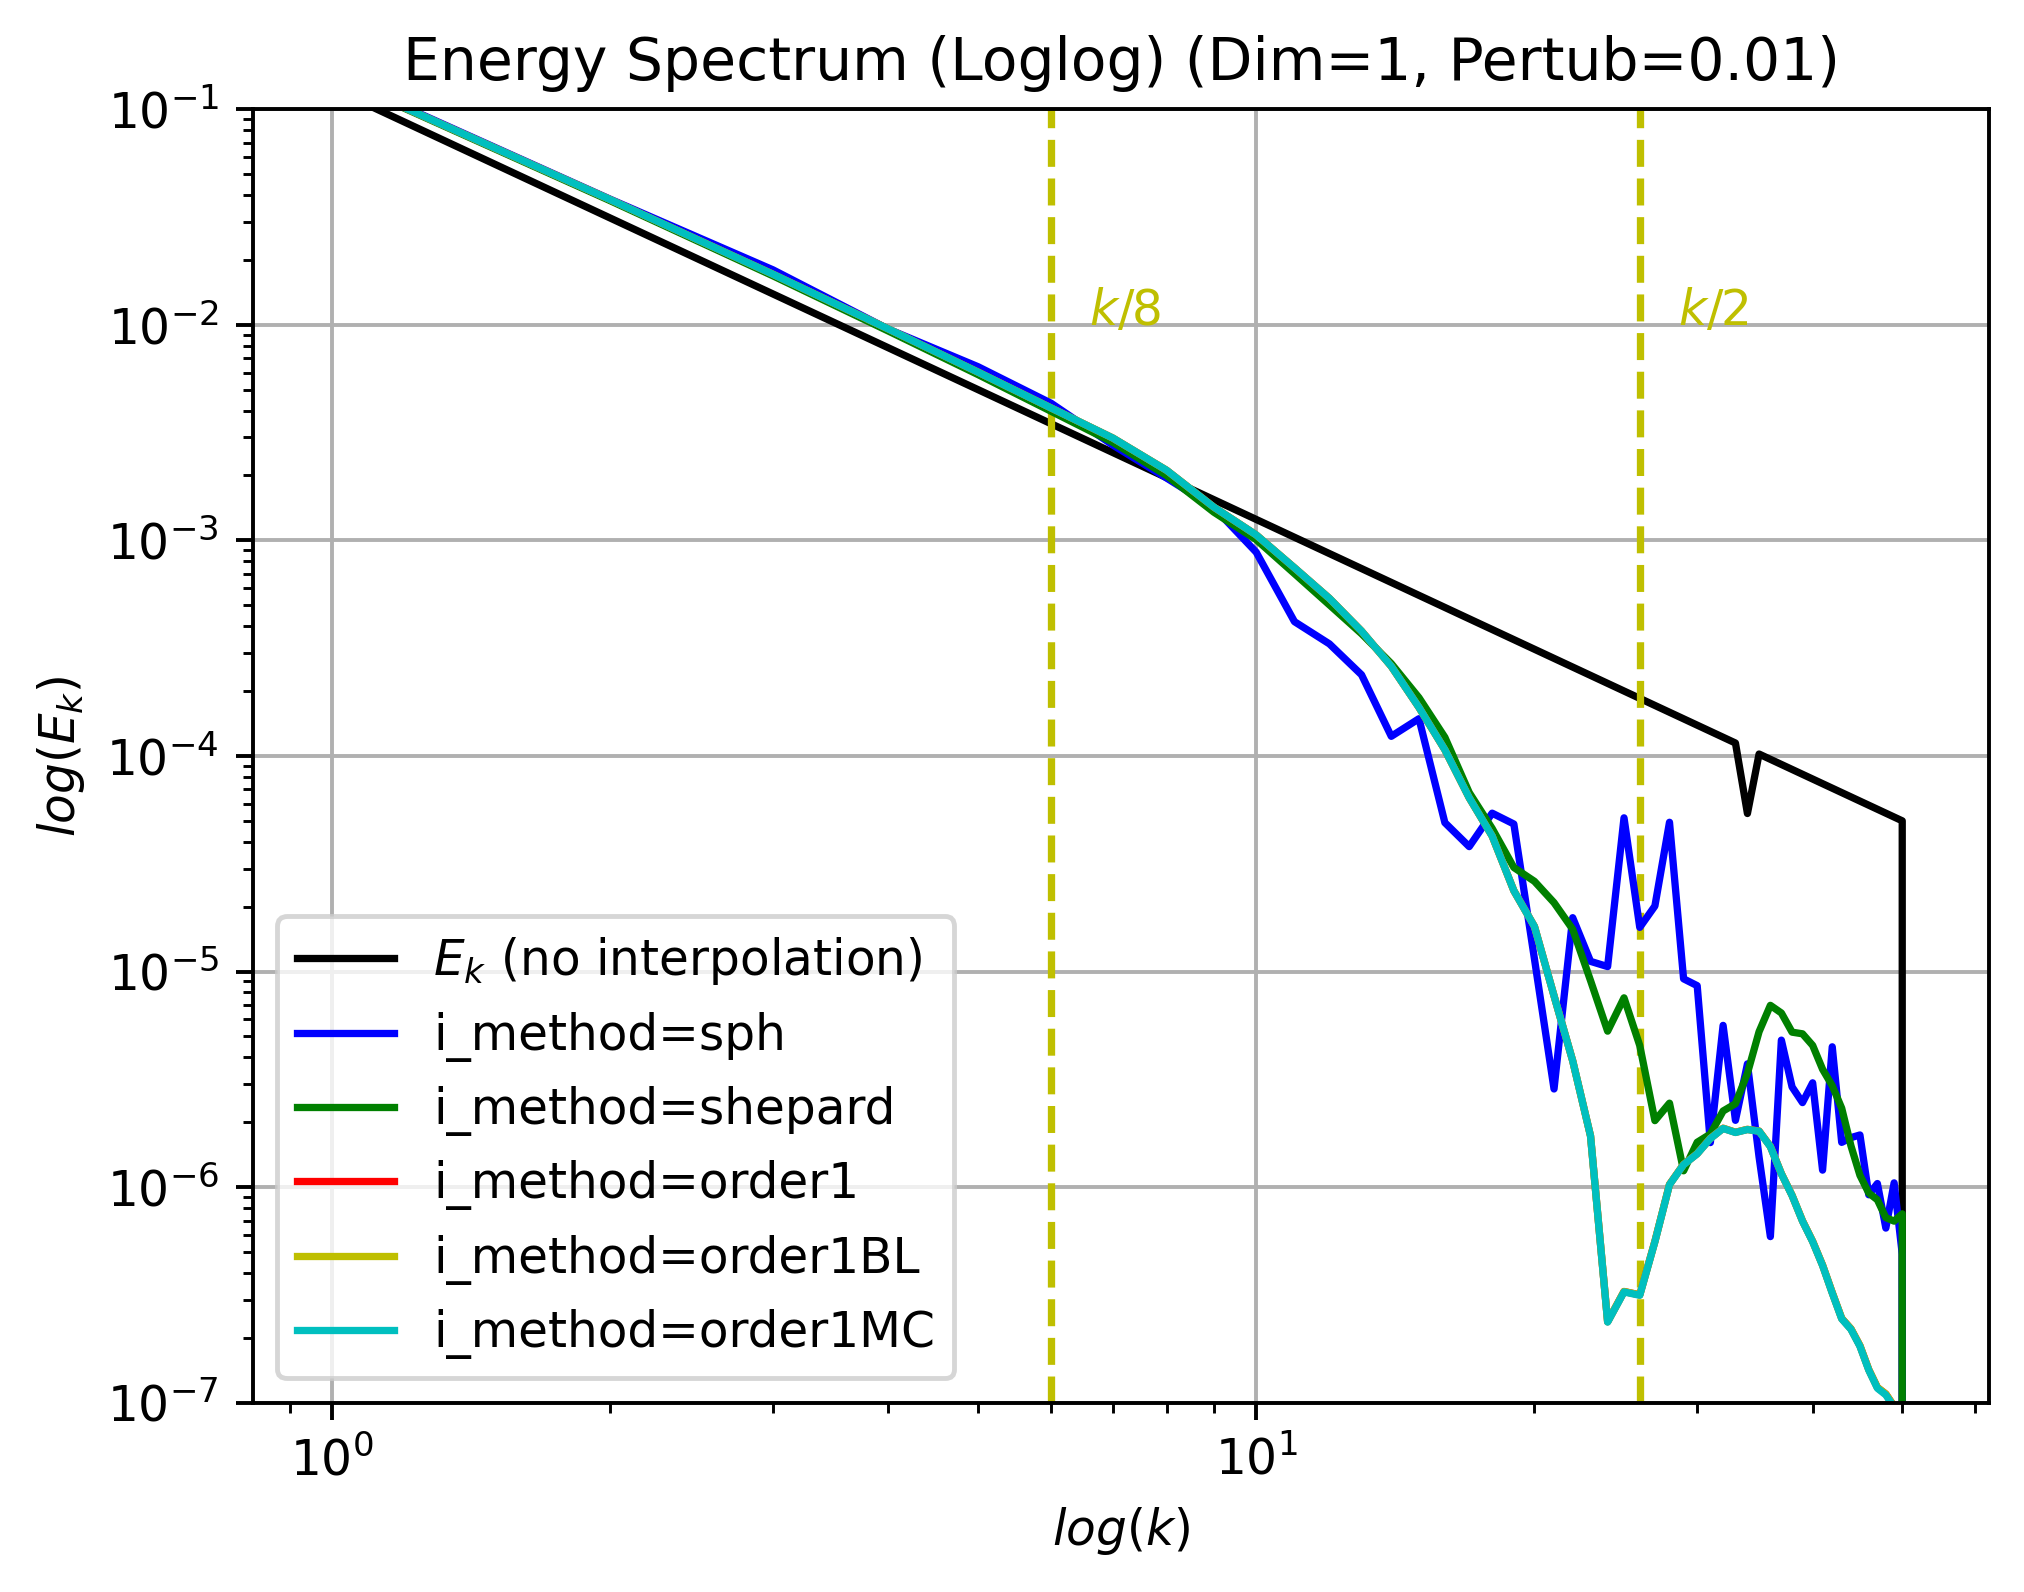
\includegraphics[width=6cm]{Code-Figures/sin-vel-prof-i-methods/Energy Spectrum (Loglog) (Dim=1, Pertub=0.01).png}
		\caption{$1D$ $E(k)$ field}
	\end{subfigure}
	\begin{subfigure}{7cm}
		\centering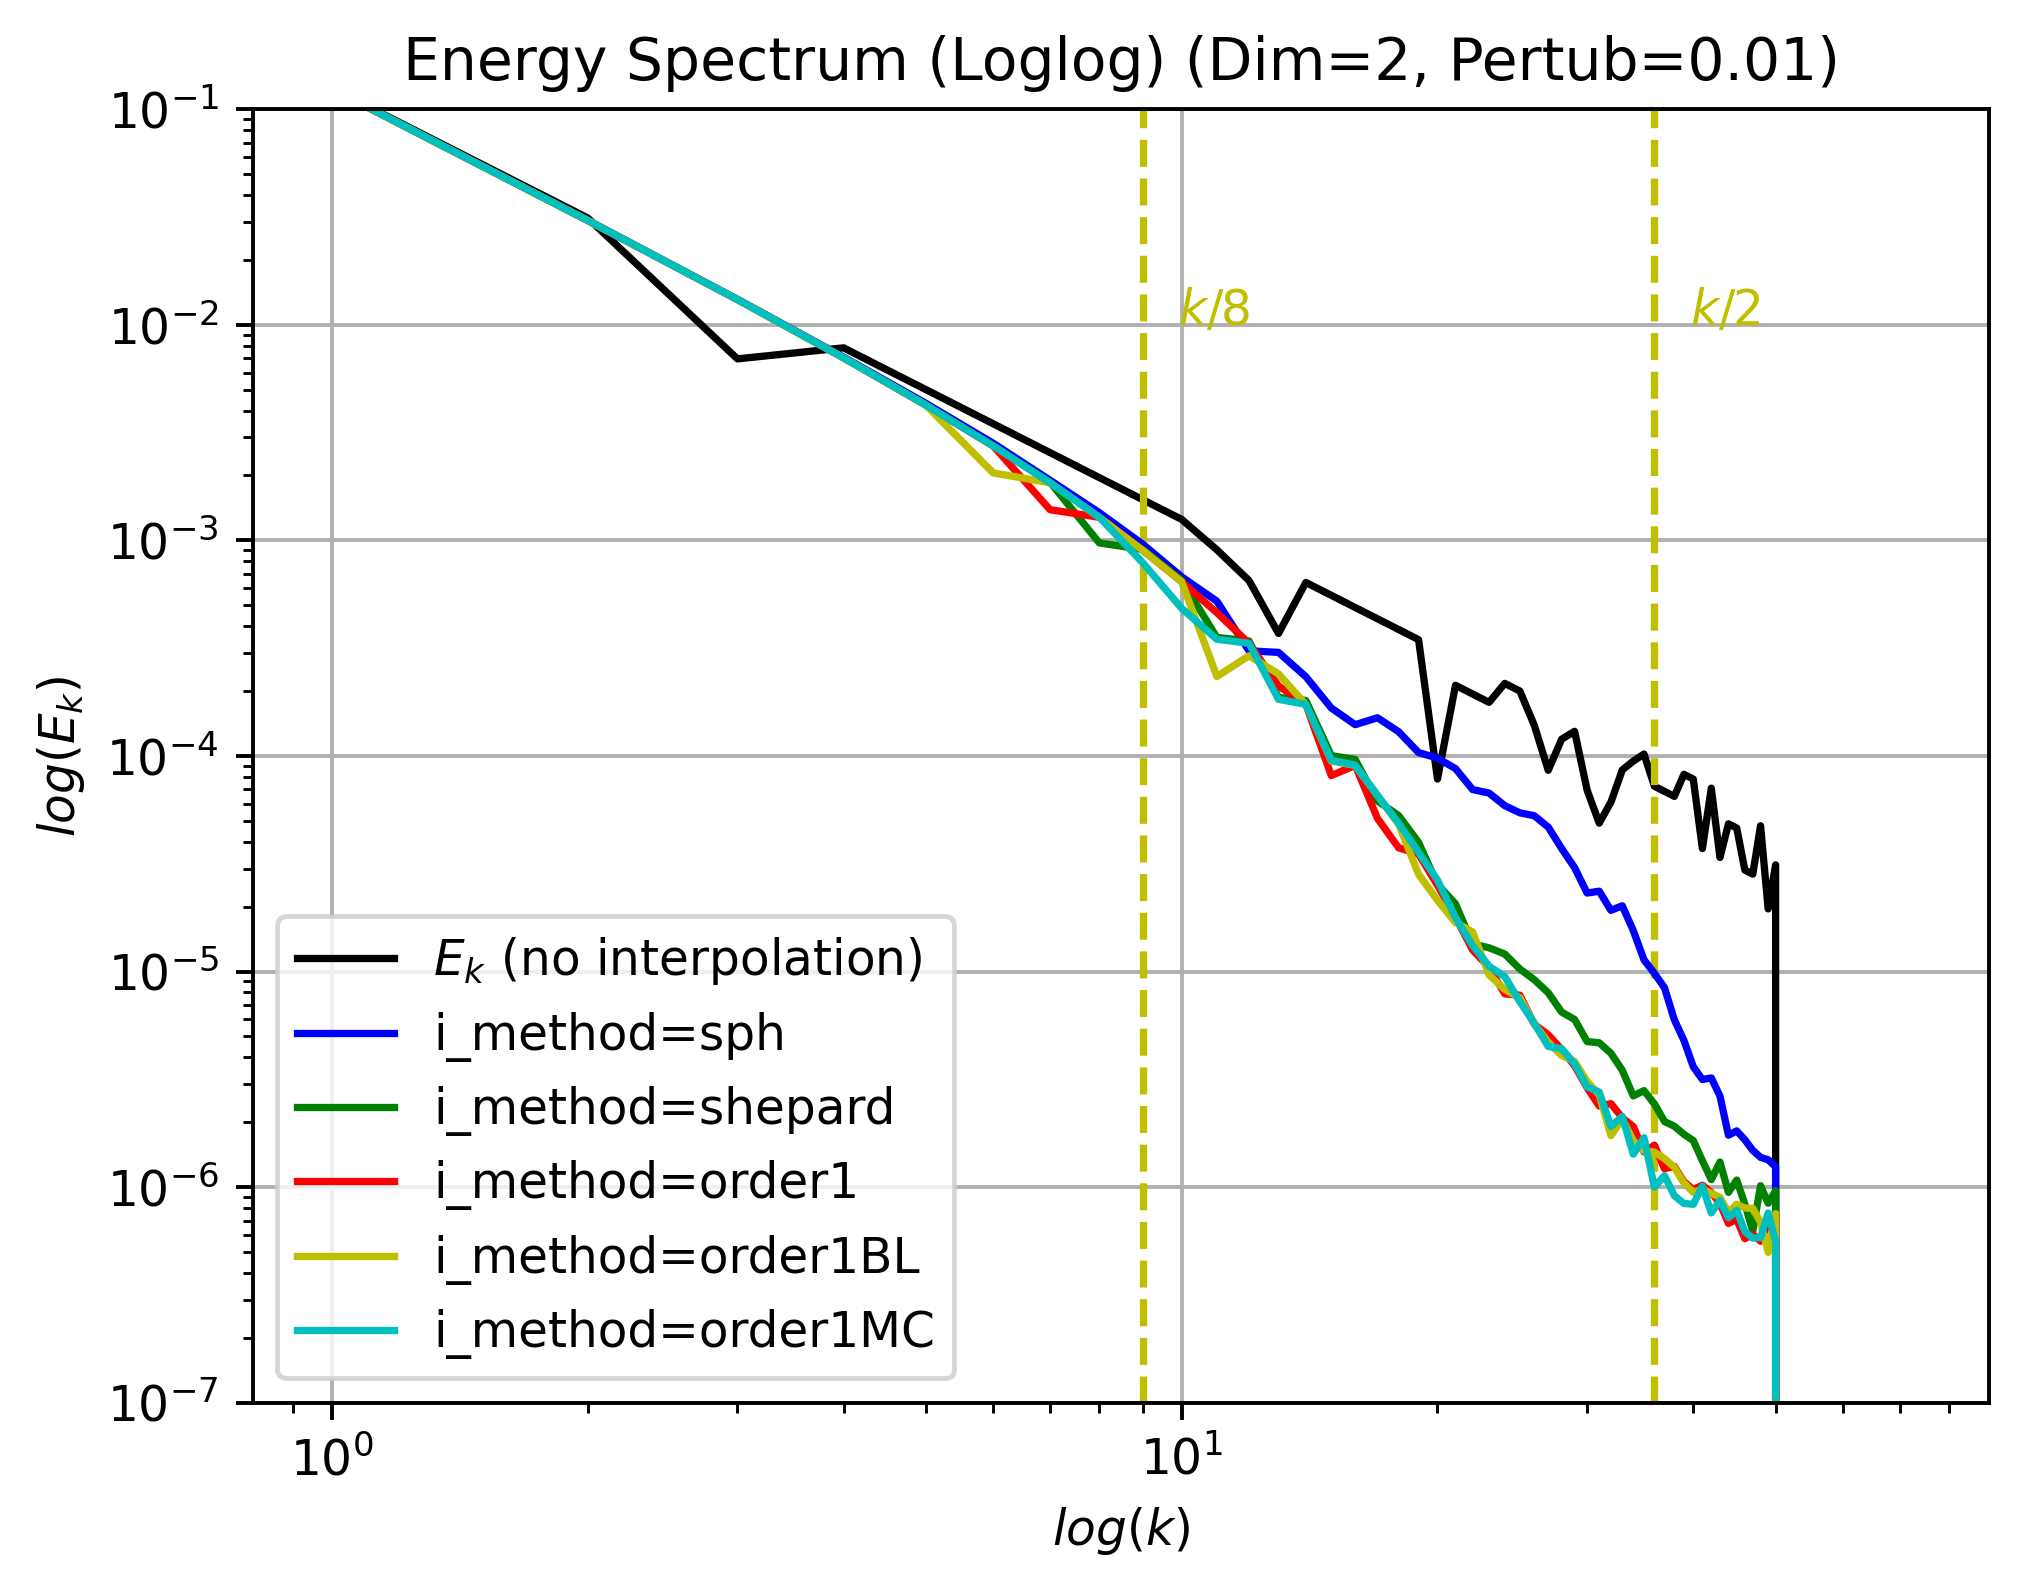
\includegraphics[width=6cm]{Code-Figures/sin-vel-prof-i-methods/Energy Spectrum (Loglog) (Dim=2, Pertub=0.01).png}
		\caption{$2D$ $E(k)$ field}
	\end{subfigure}
	\begin{subfigure}{7cm}
		\centering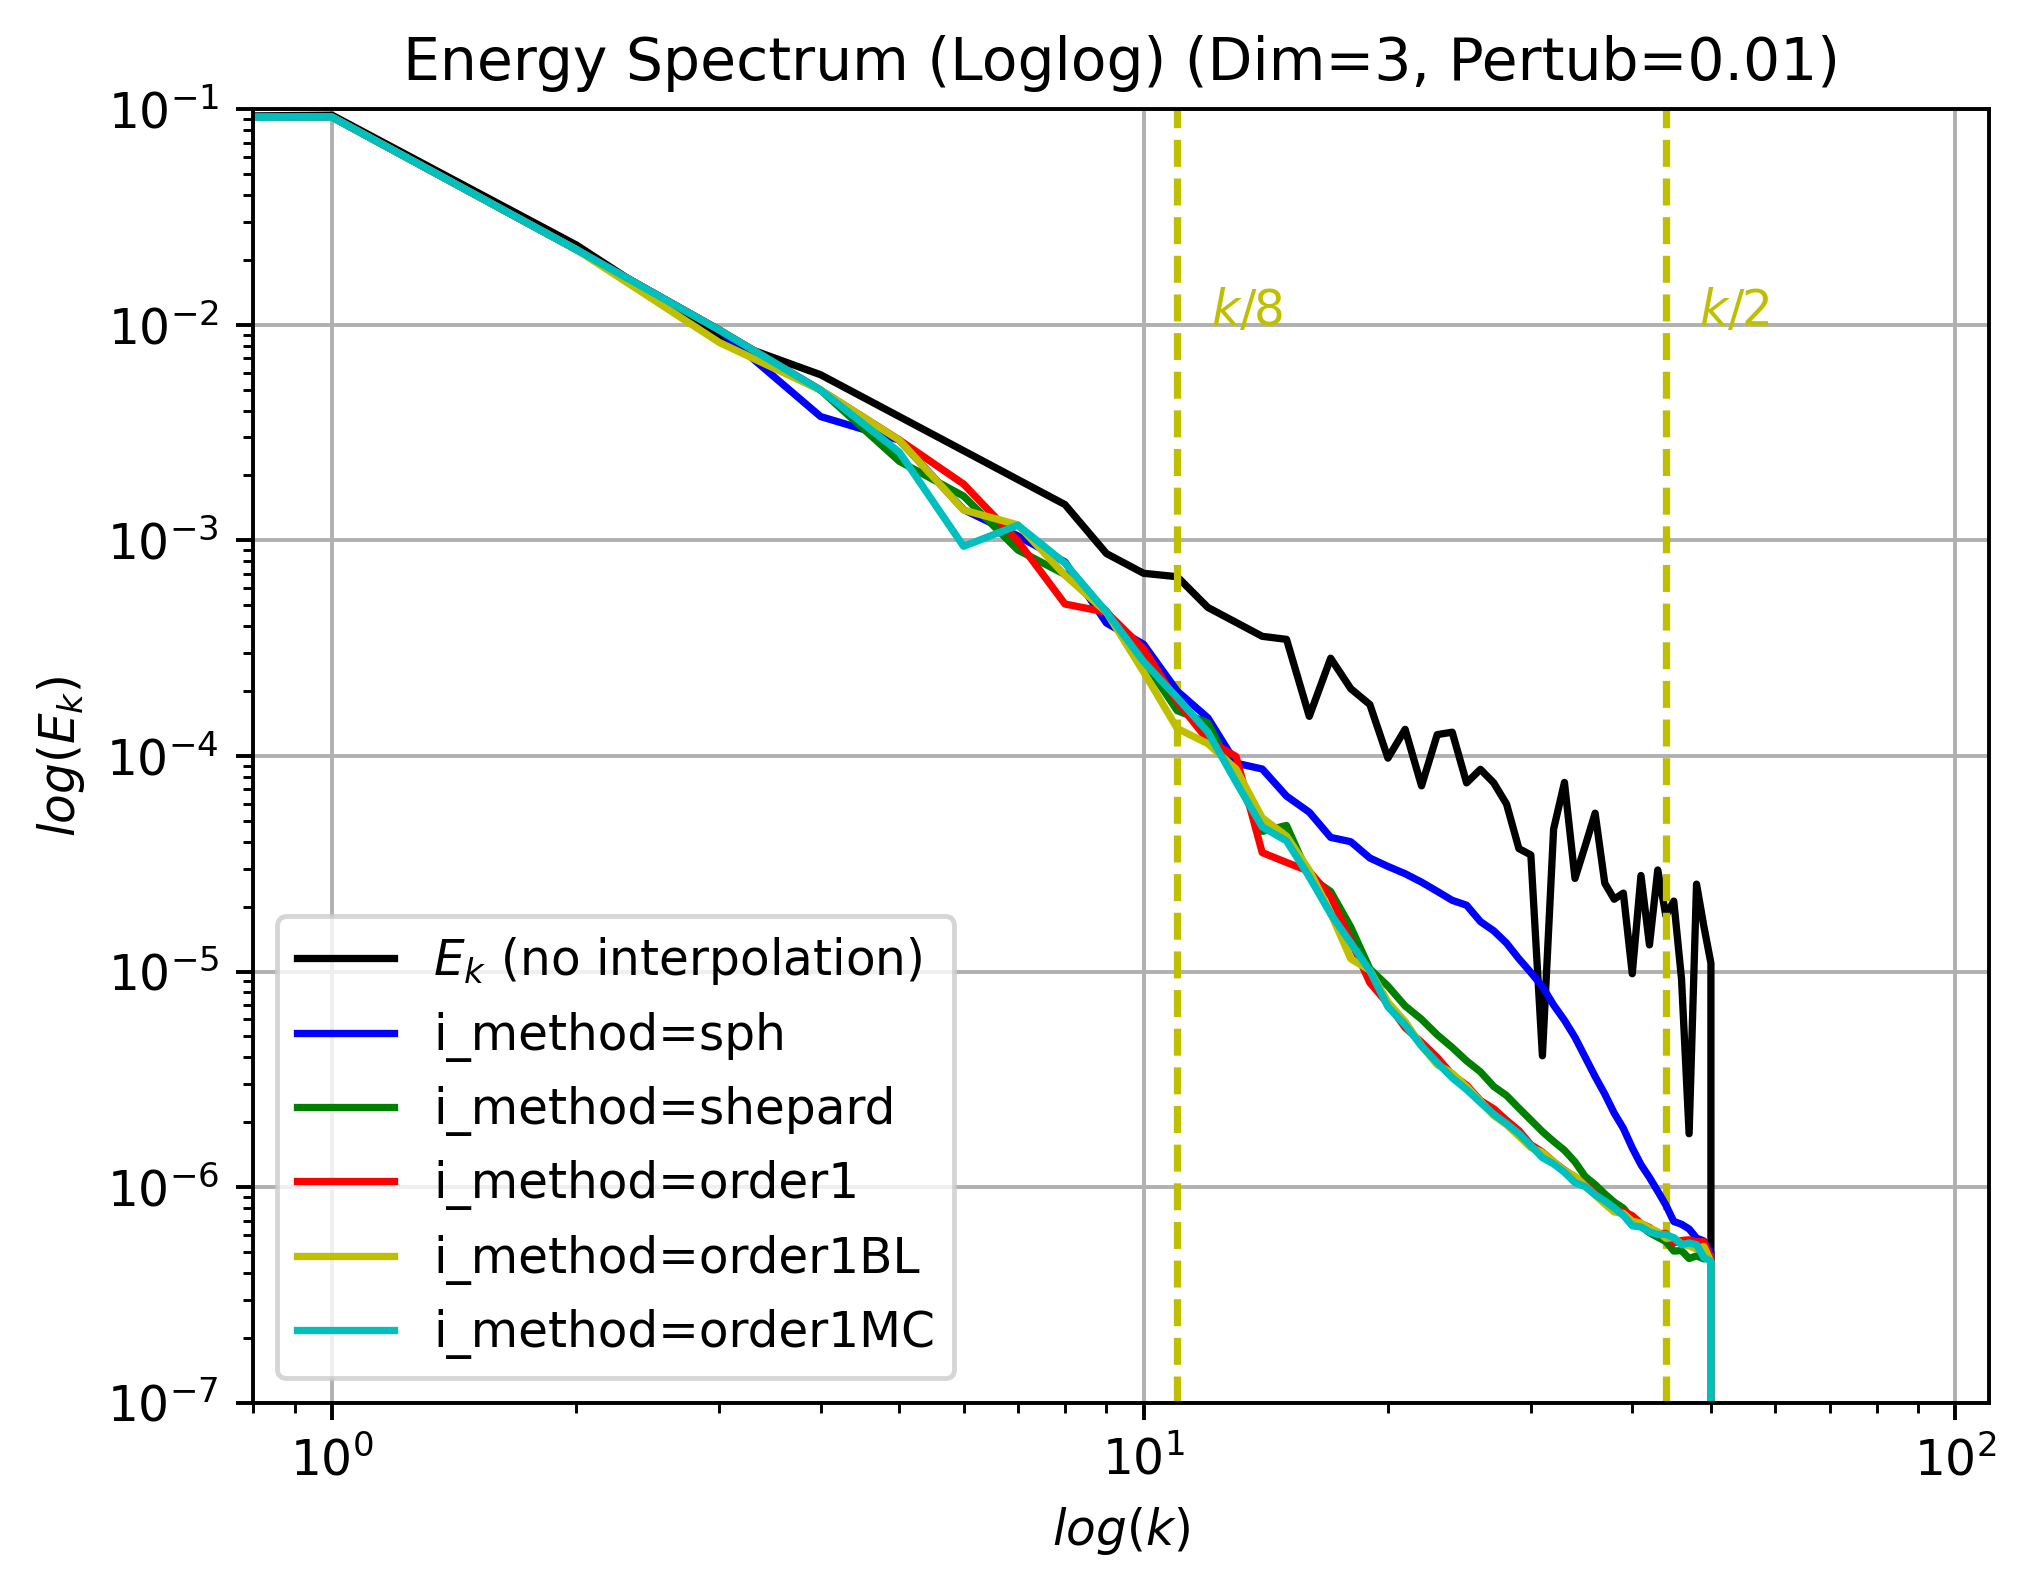
\includegraphics[width=6cm]{Code-Figures/sin-vel-prof-i-methods/Energy Spectrum (Loglog) (Dim=3, Pertub=0.01).png}
		\caption{$3D$ $E(k)$ field}
	\end{subfigure}
	\caption{The scalar fields $E(k)$ for $1D$, $2D$, and $3D$ case, for various interpolation schemes.}
	\label{fig:espec-scalar-fields-i-methods}
\end{figure}

Then, in order to measure the effect of the kernel on the computed energy spectrum, the following kernels were considered:
\begin{itemize}
    \item \texttt{CubicSpline},
    \item \texttt{WendlandQuinticC2},
    \item \texttt{WendlandQuinticC4},
    \item \texttt{WendlandQuinticC6},
    \item \texttt{Gaussian},
    \item \texttt{SuperGaussian},
    \item \texttt{QuinticSpline}.
\end{itemize}

From the results shown in \figref{fig:espec-scalar-fields-i-kernels}, it can be observed thatall kernels underestimate the energy at lower length scales, with the \texttt{Gaussian} kernel underestimating the most.
The \texttt{WendlandQuinticC6} kernel seems to predict the energy spectrum closest to the exact trend, which holds for all dimensions.
Therefore, the \texttt{WendlandQuinticC6} kernel is chosen as the default kernel for the computation of the energy spectrum.

\begin{figure}[htbp!]
	\begin{subfigure}{7cm}
		\centering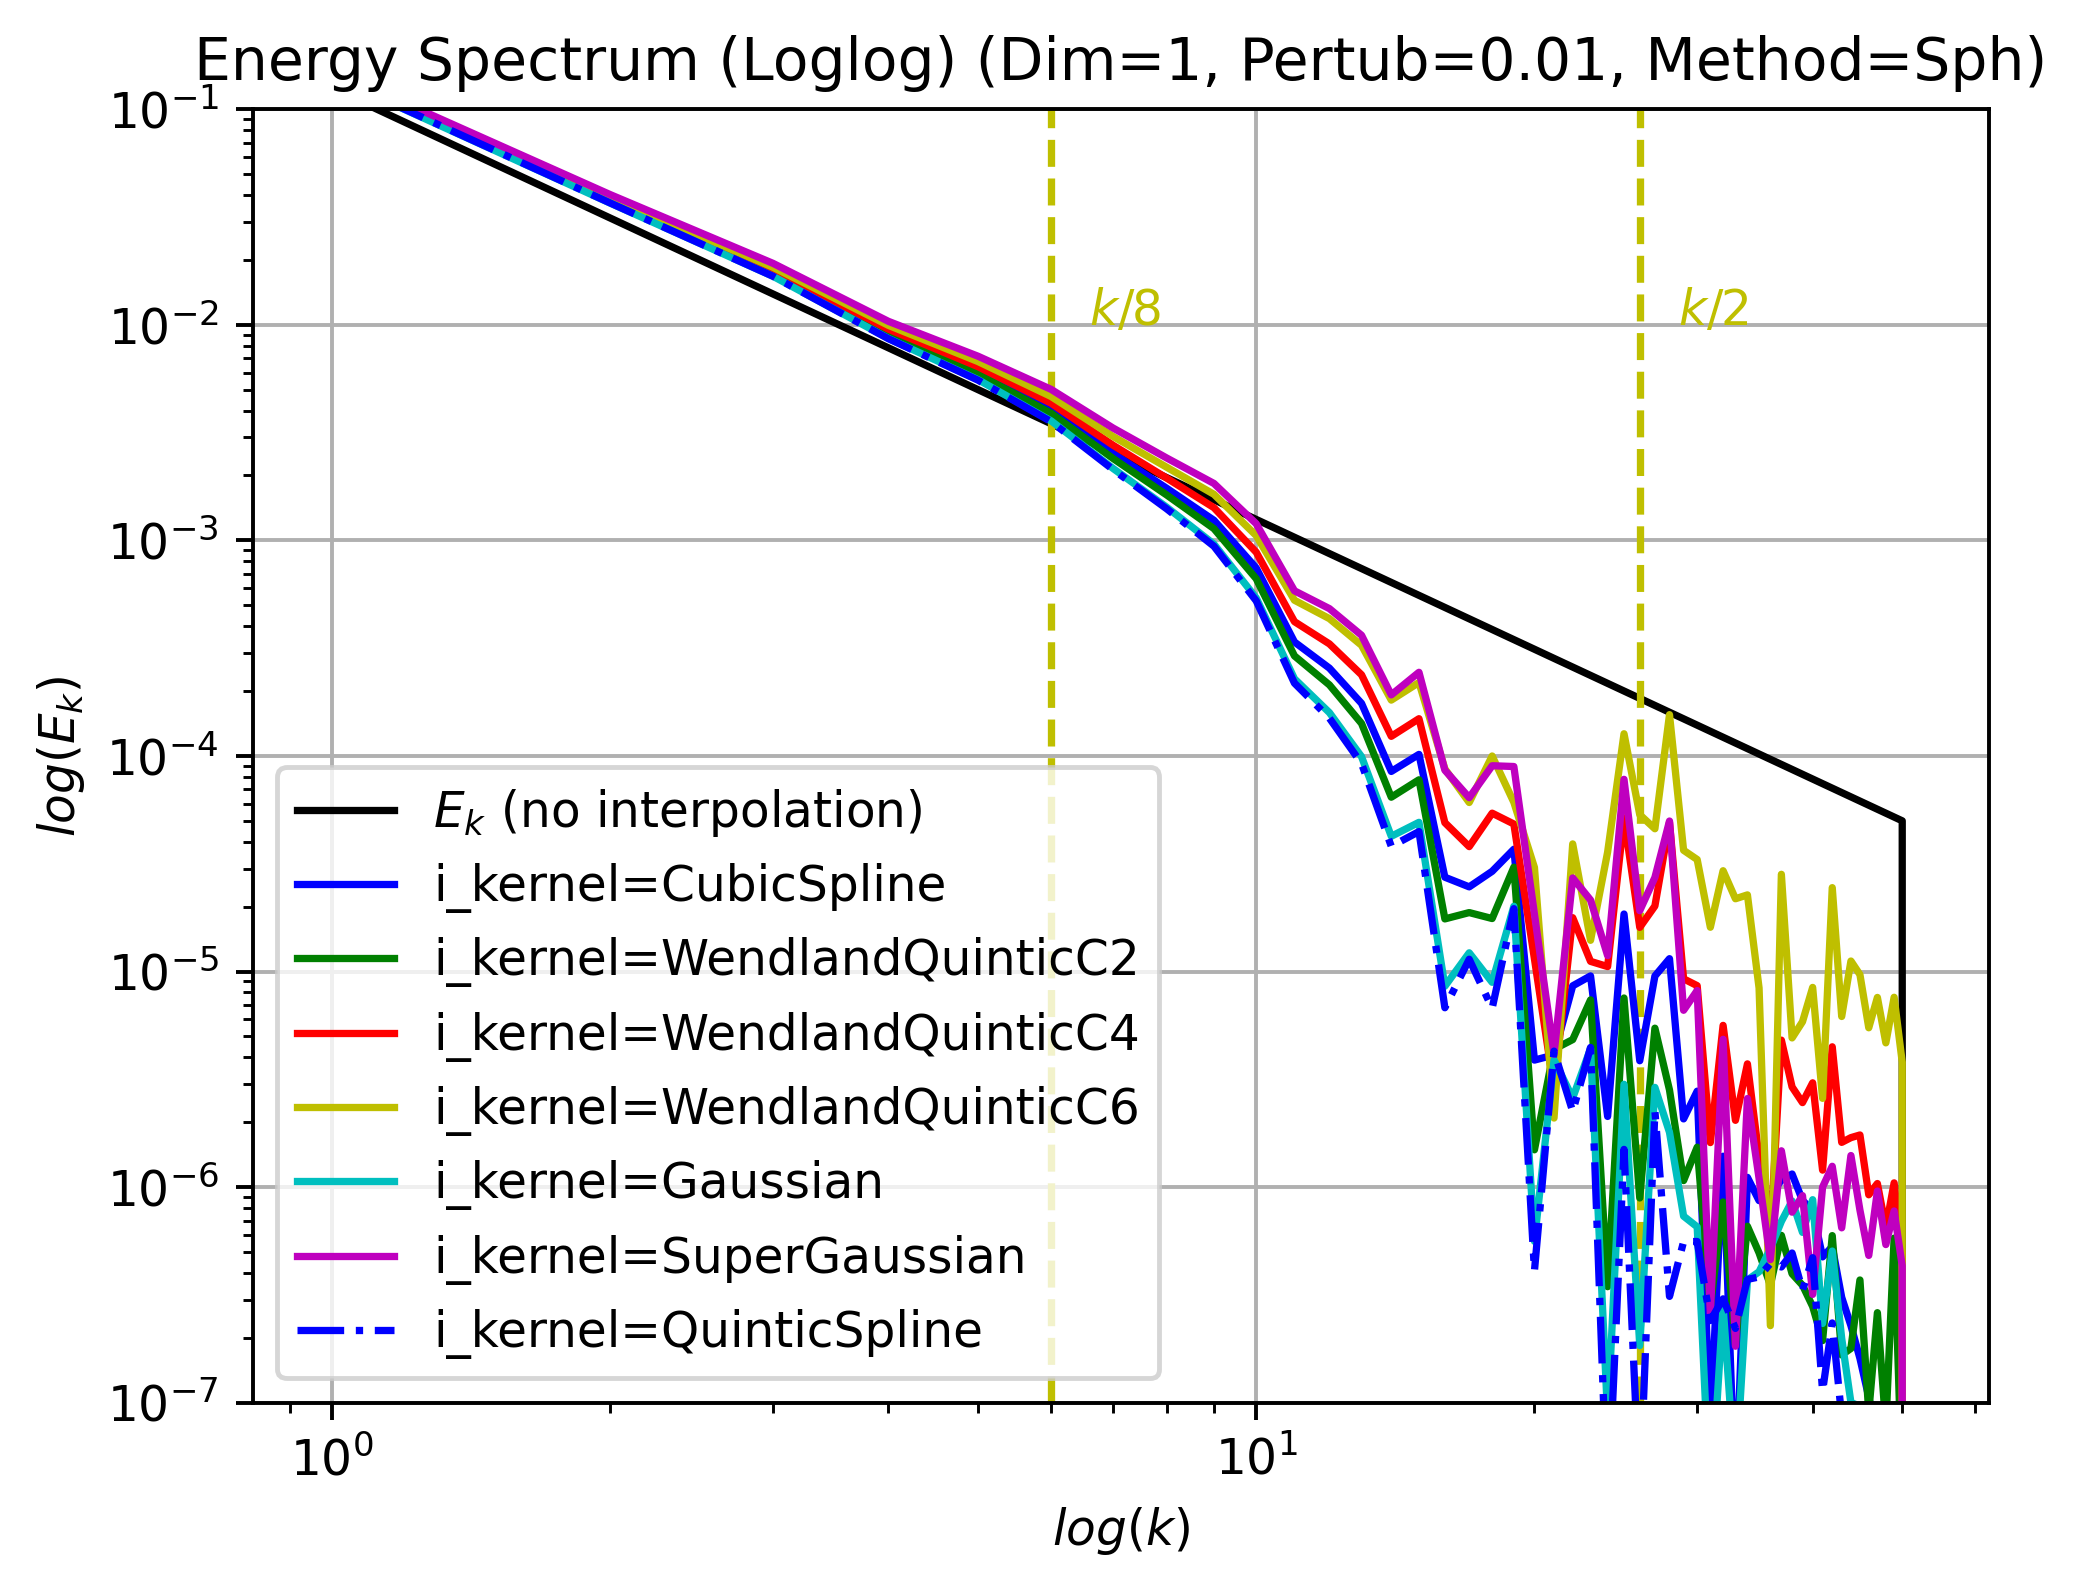
\includegraphics[width=6cm]{Code-Figures/sin-vel-prof-i-kernel/Energy Spectrum (Loglog) (Dim=1, Pertub=0.01, Method=Sph).png}
		\caption{$1D$ $E(k)$ field}
	\end{subfigure}
	\begin{subfigure}{7cm}
		\centering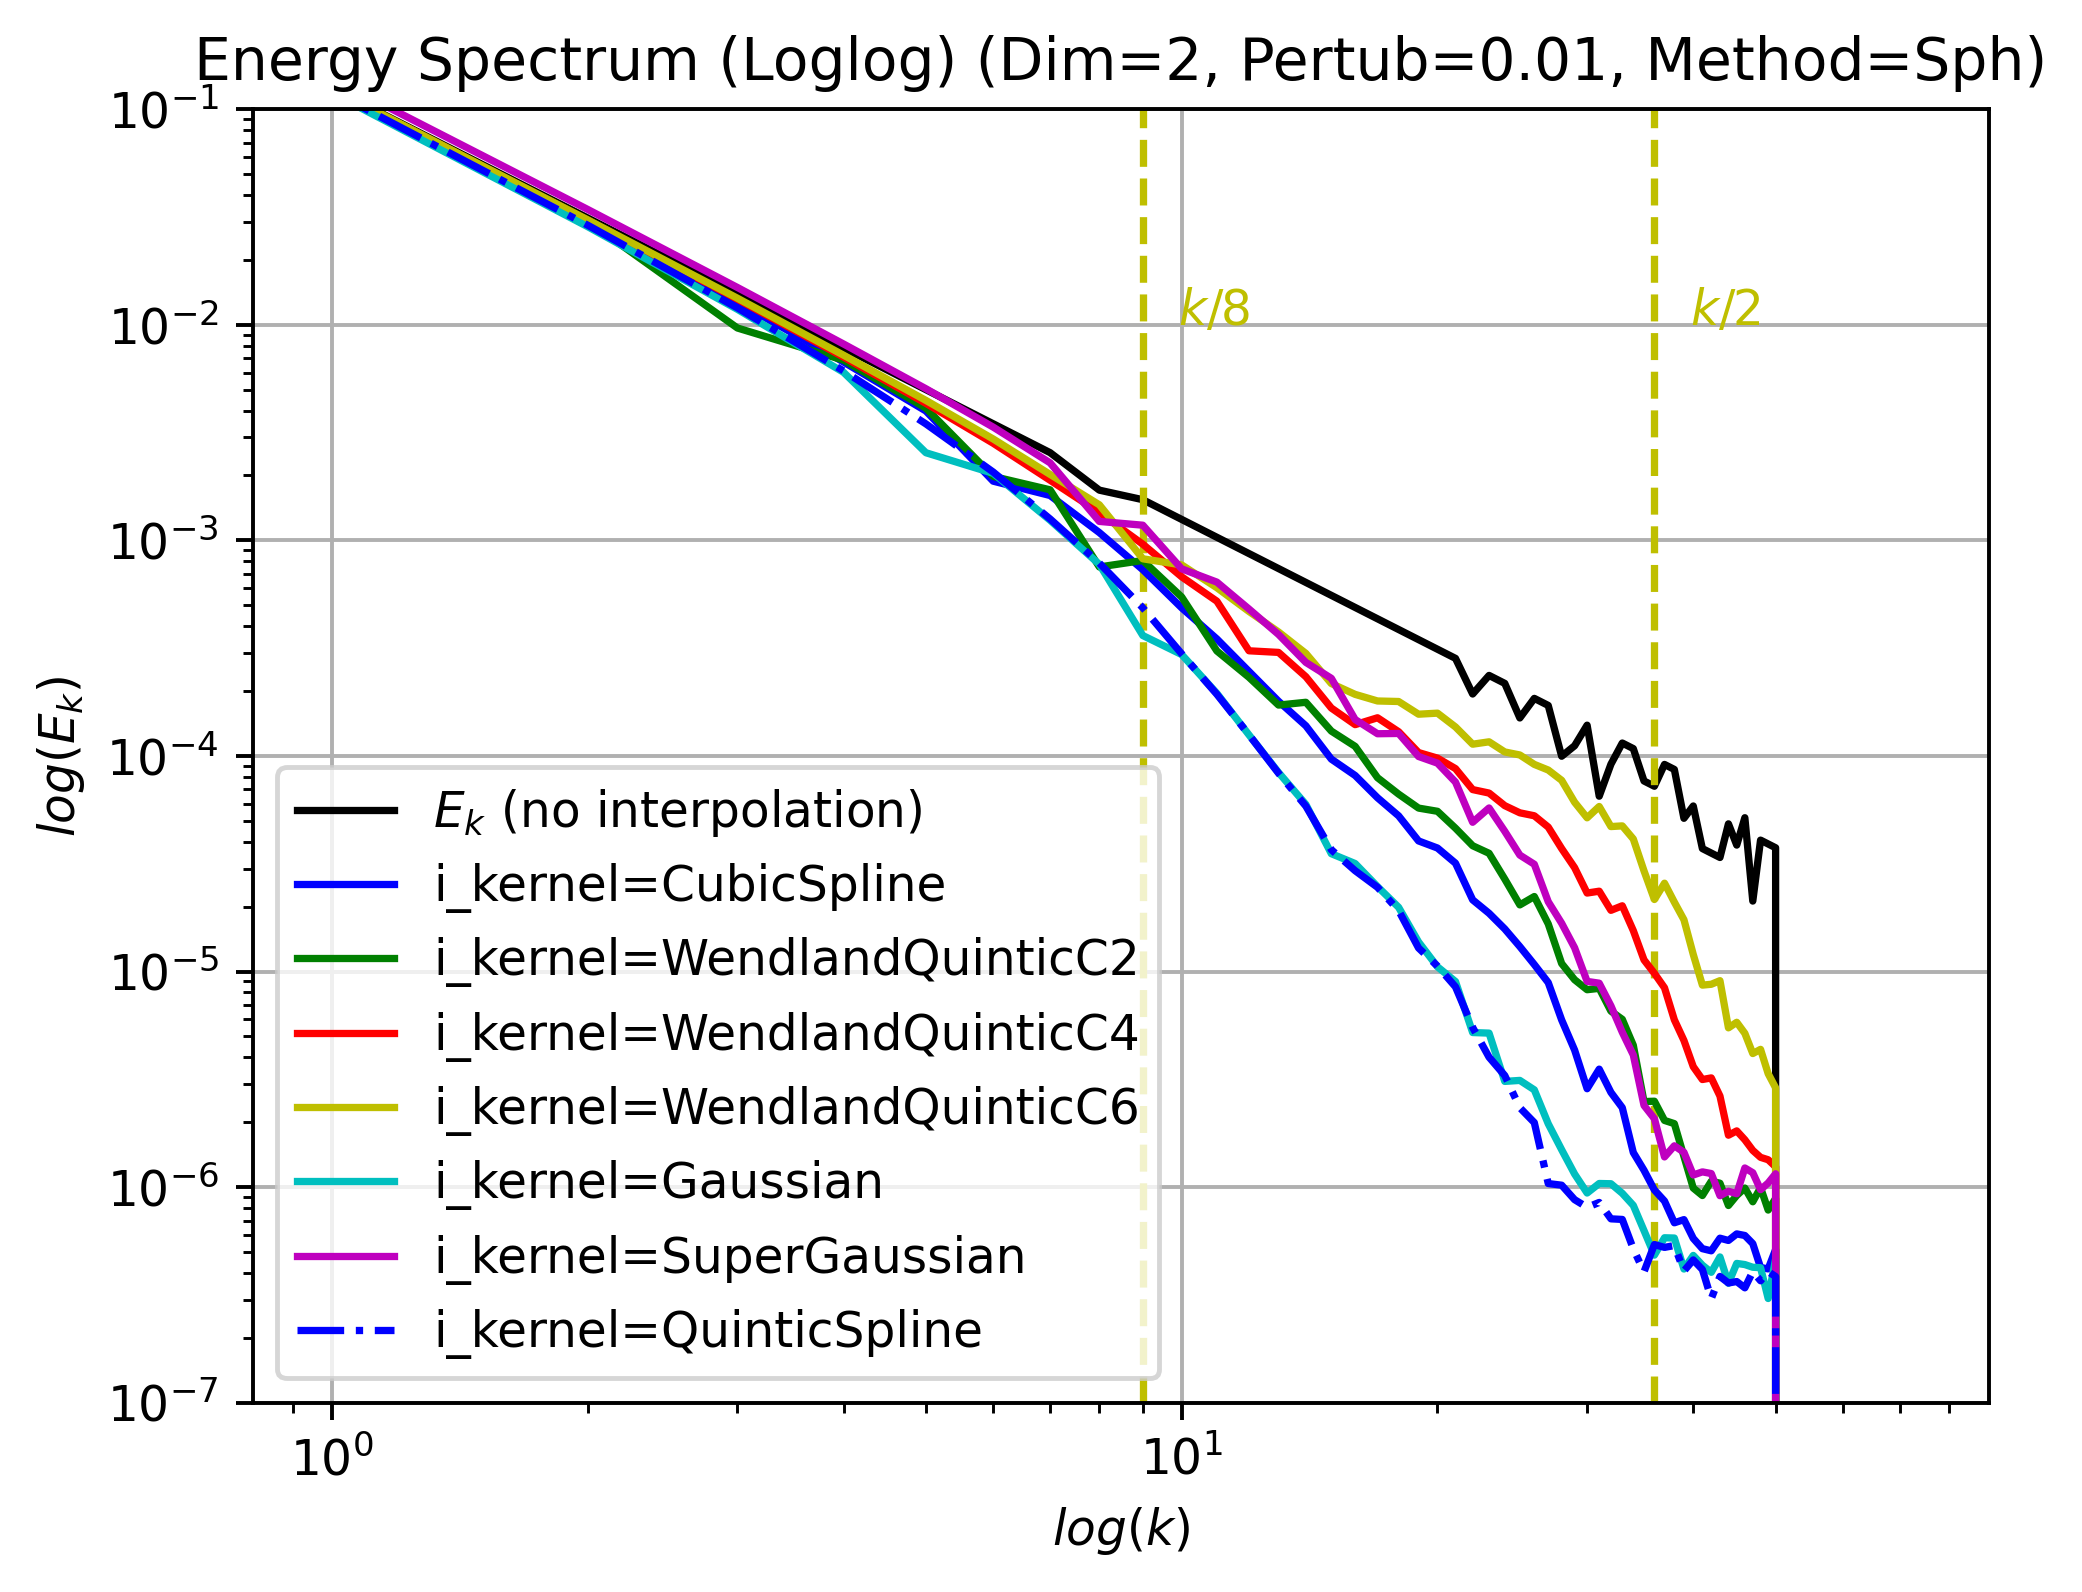
\includegraphics[width=6cm]{Code-Figures/sin-vel-prof-i-kernel/Energy Spectrum (Loglog) (Dim=2, Pertub=0.01, Method=Sph).png}
		\caption{$2D$ $E(k)$ field}
	\end{subfigure}
	\begin{subfigure}{7cm}
		\centering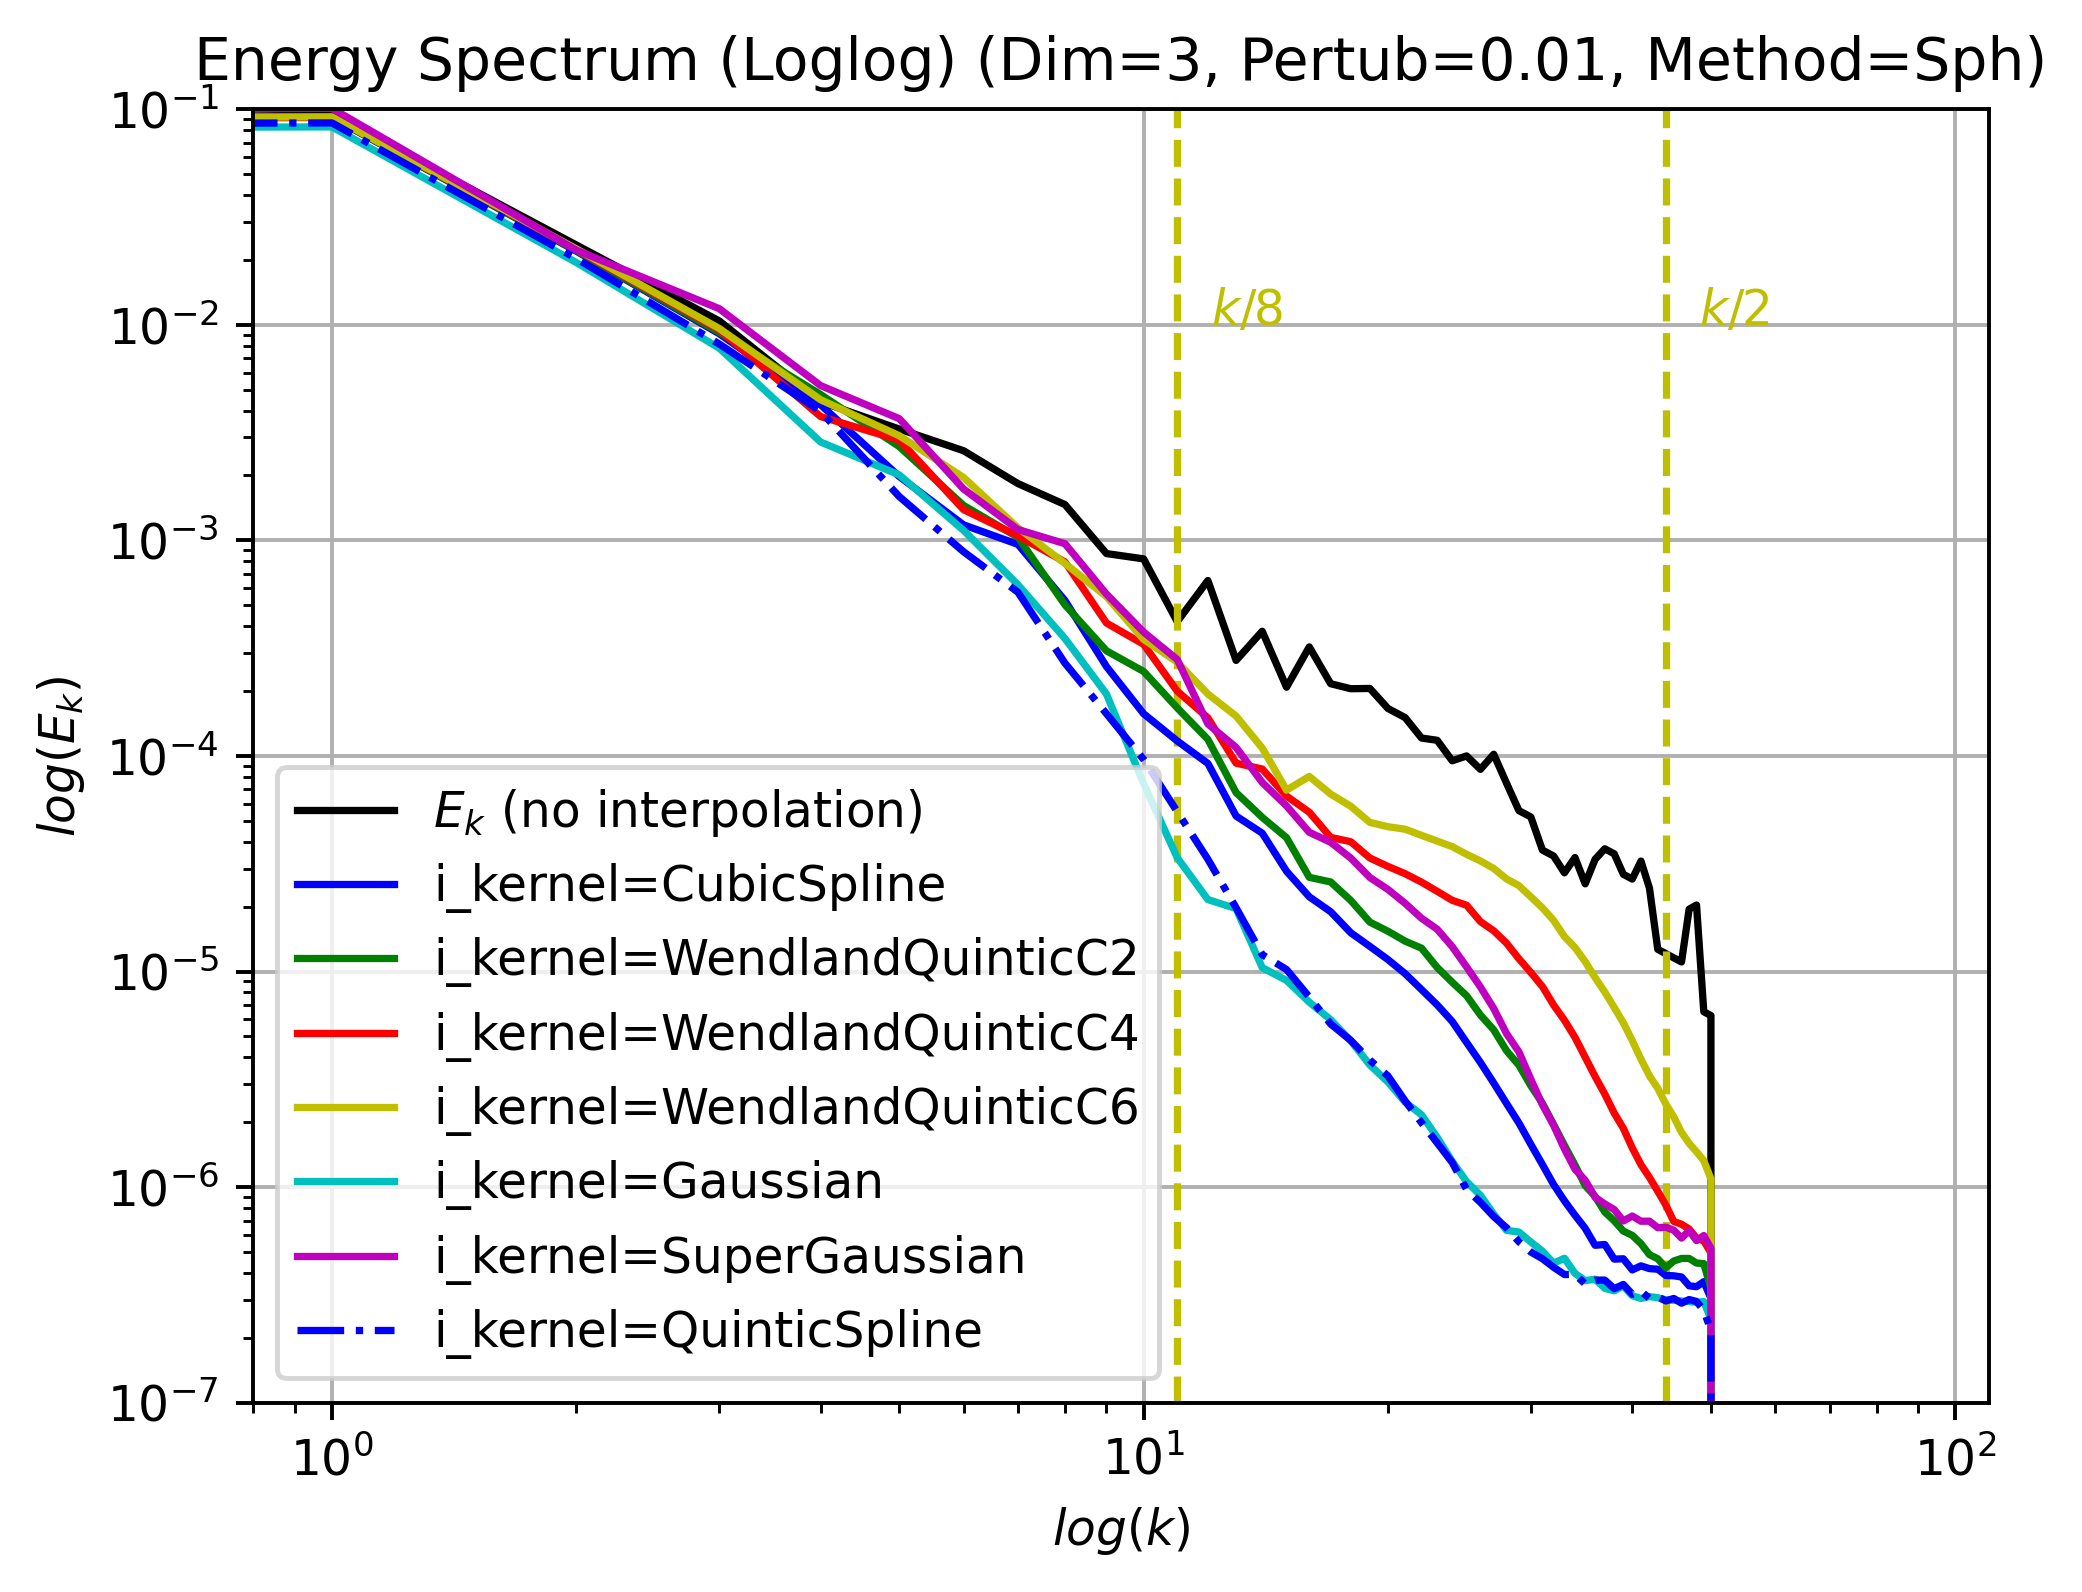
\includegraphics[width=6cm]{Code-Figures/sin-vel-prof-i-kernel/Energy Spectrum (Loglog) (Dim=3, Pertub=0.01, Method=Sph).png}
		\caption{$3D$ $E(k)$ field}
	\end{subfigure}
	\caption{The scalar fields $E(k)$ for $1D$, $2D$, and $3D$ case, for various interpolation kernels.}
	\label{fig:espec-scalar-fields-i-kernels}
\end{figure}

Finally, in order to measure the effect of particle resolution on the computed energy spectrum, test cases with a $\gamma=1$ and $N=30$ were considered for all dimensions, with the range of the number of particles along each axis being $[61, 91, 121]$.
From the results shown in \figref{fig:espec-scalar-fields-res}, it can be observed that the energy spectrum computed for the highest resolution is observed to be the closest to the exact trend for all dimensions.

\begin{figure}[htbp!]
	\begin{subfigure}{7cm}
		\centering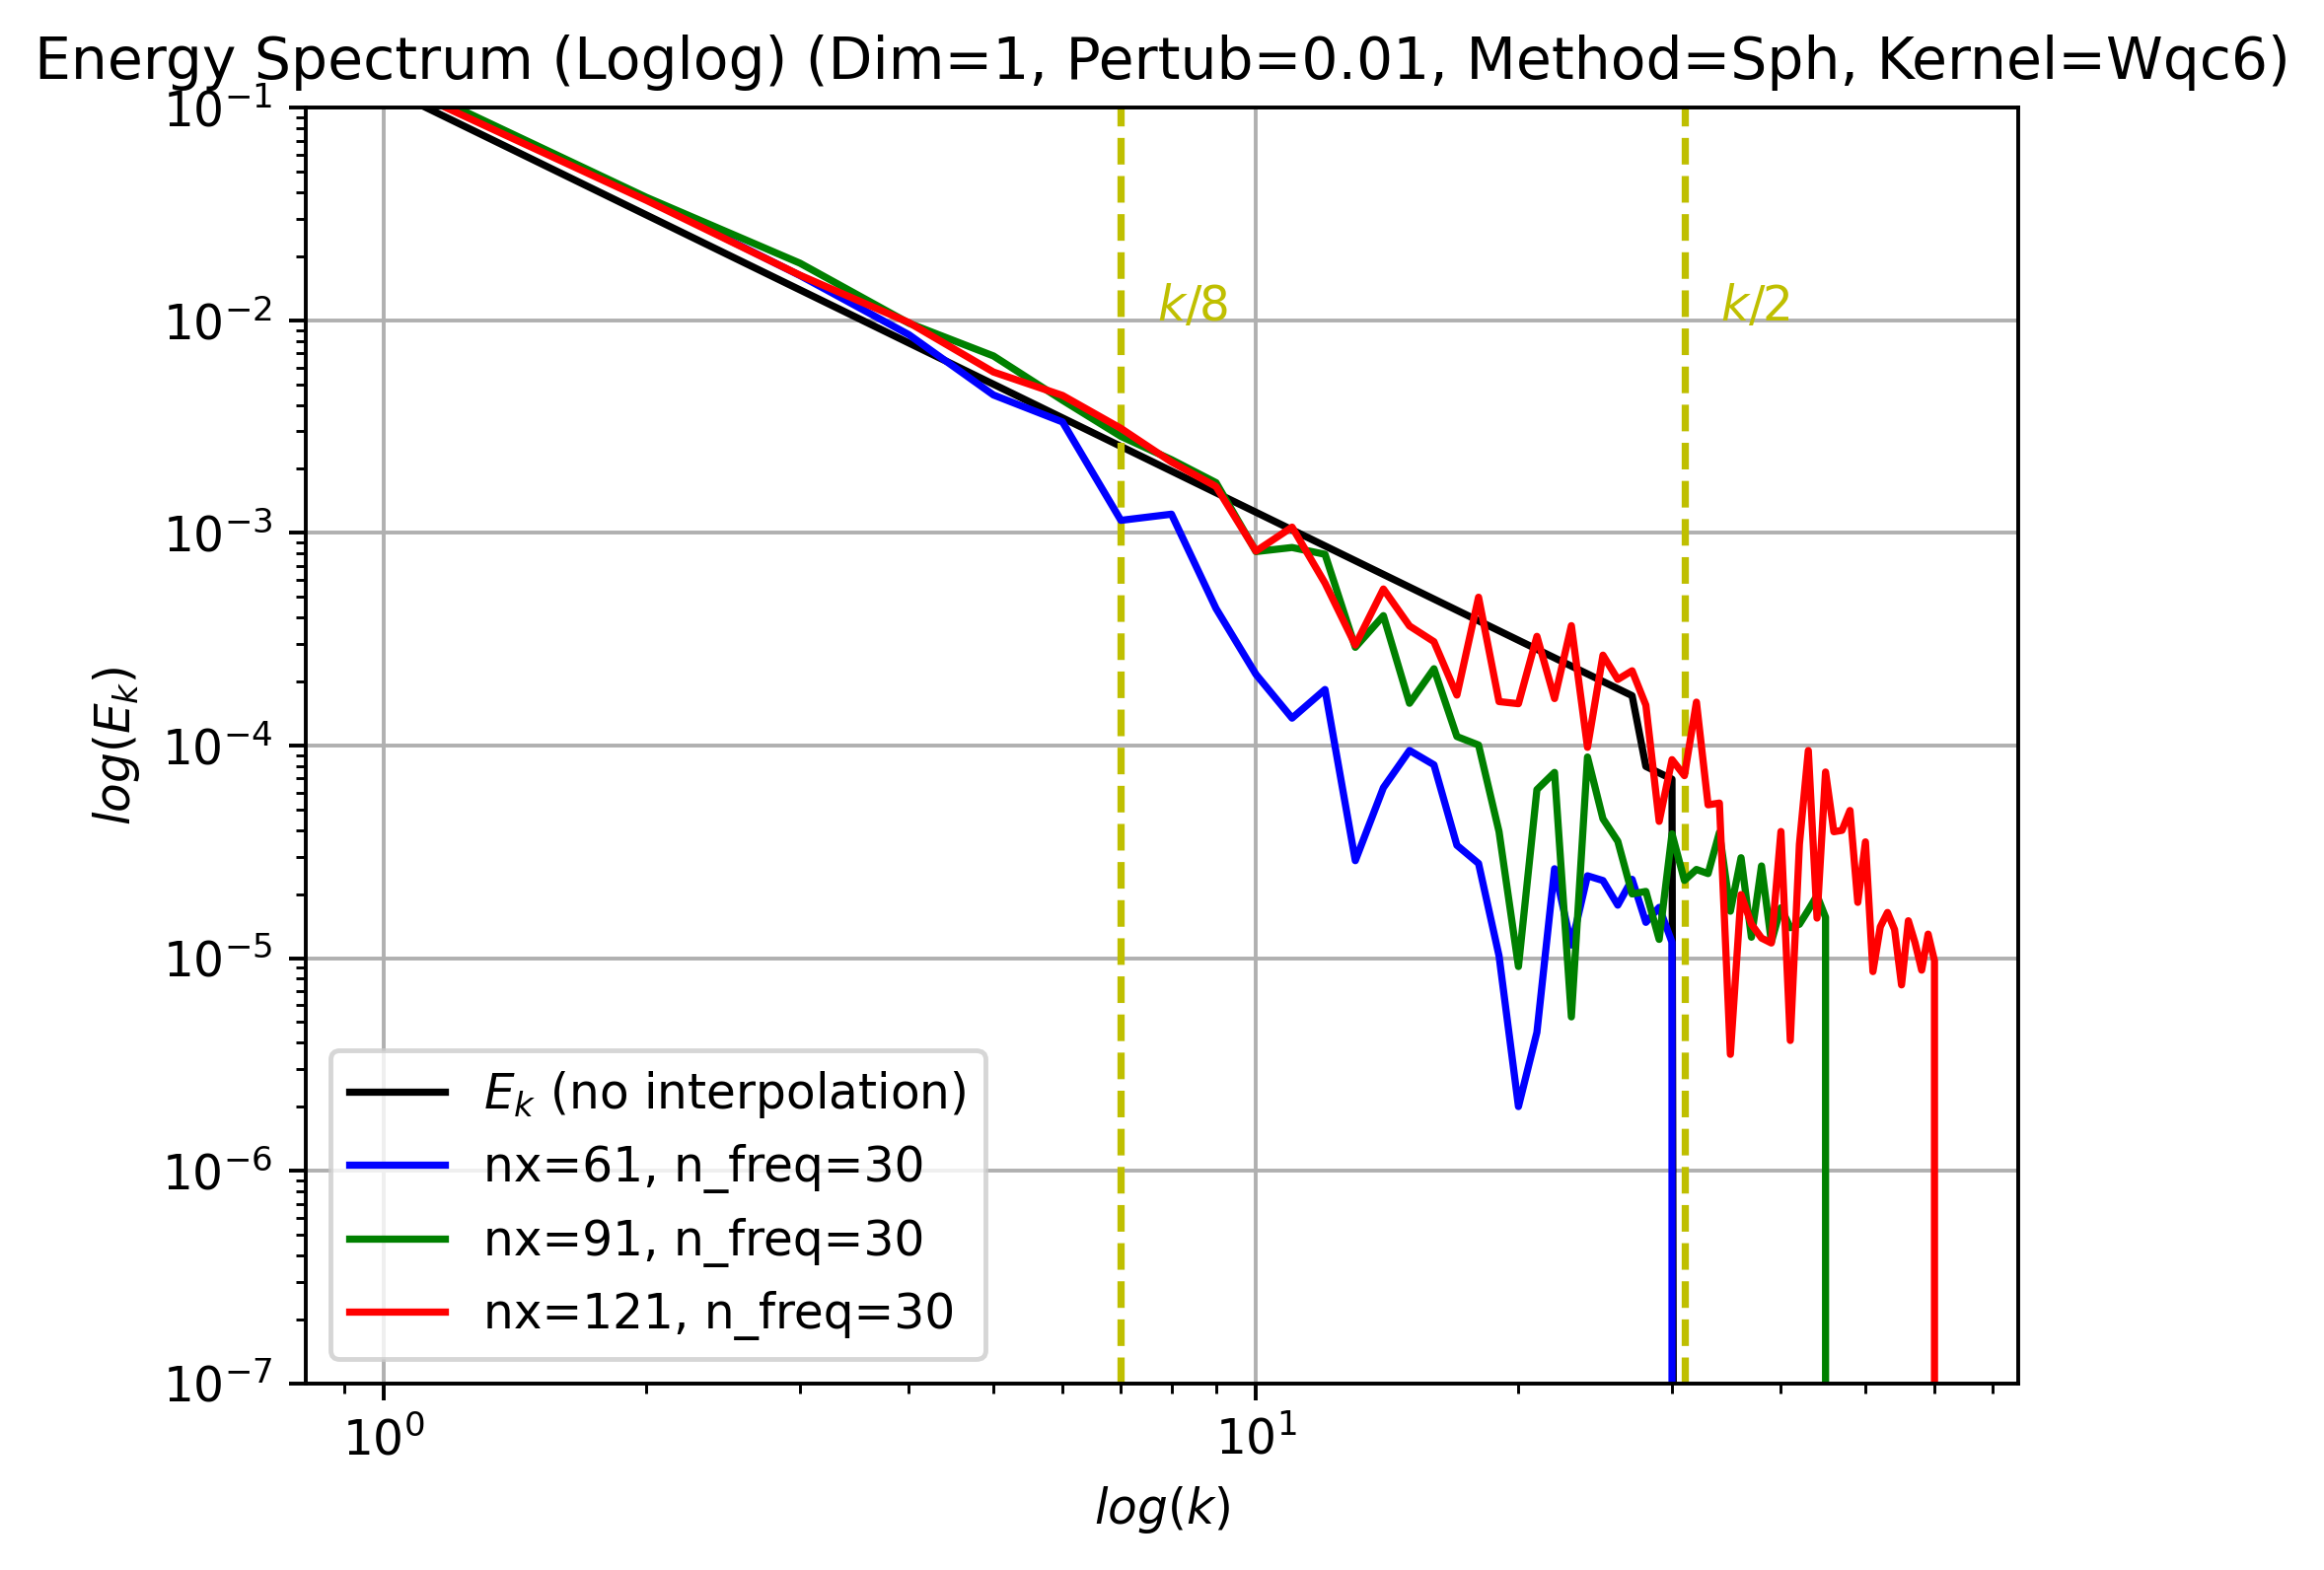
\includegraphics[width=6cm]{Code-Figures/sin-vel-prof-res/Energy Spectrum (Loglog) (Dim=1, Pertub=0.01, Method=Sph, Kernel=Wqc6).png}
		\caption{$1D$ $E(k)$ field}
	\end{subfigure}
	\begin{subfigure}{7cm}
		\centering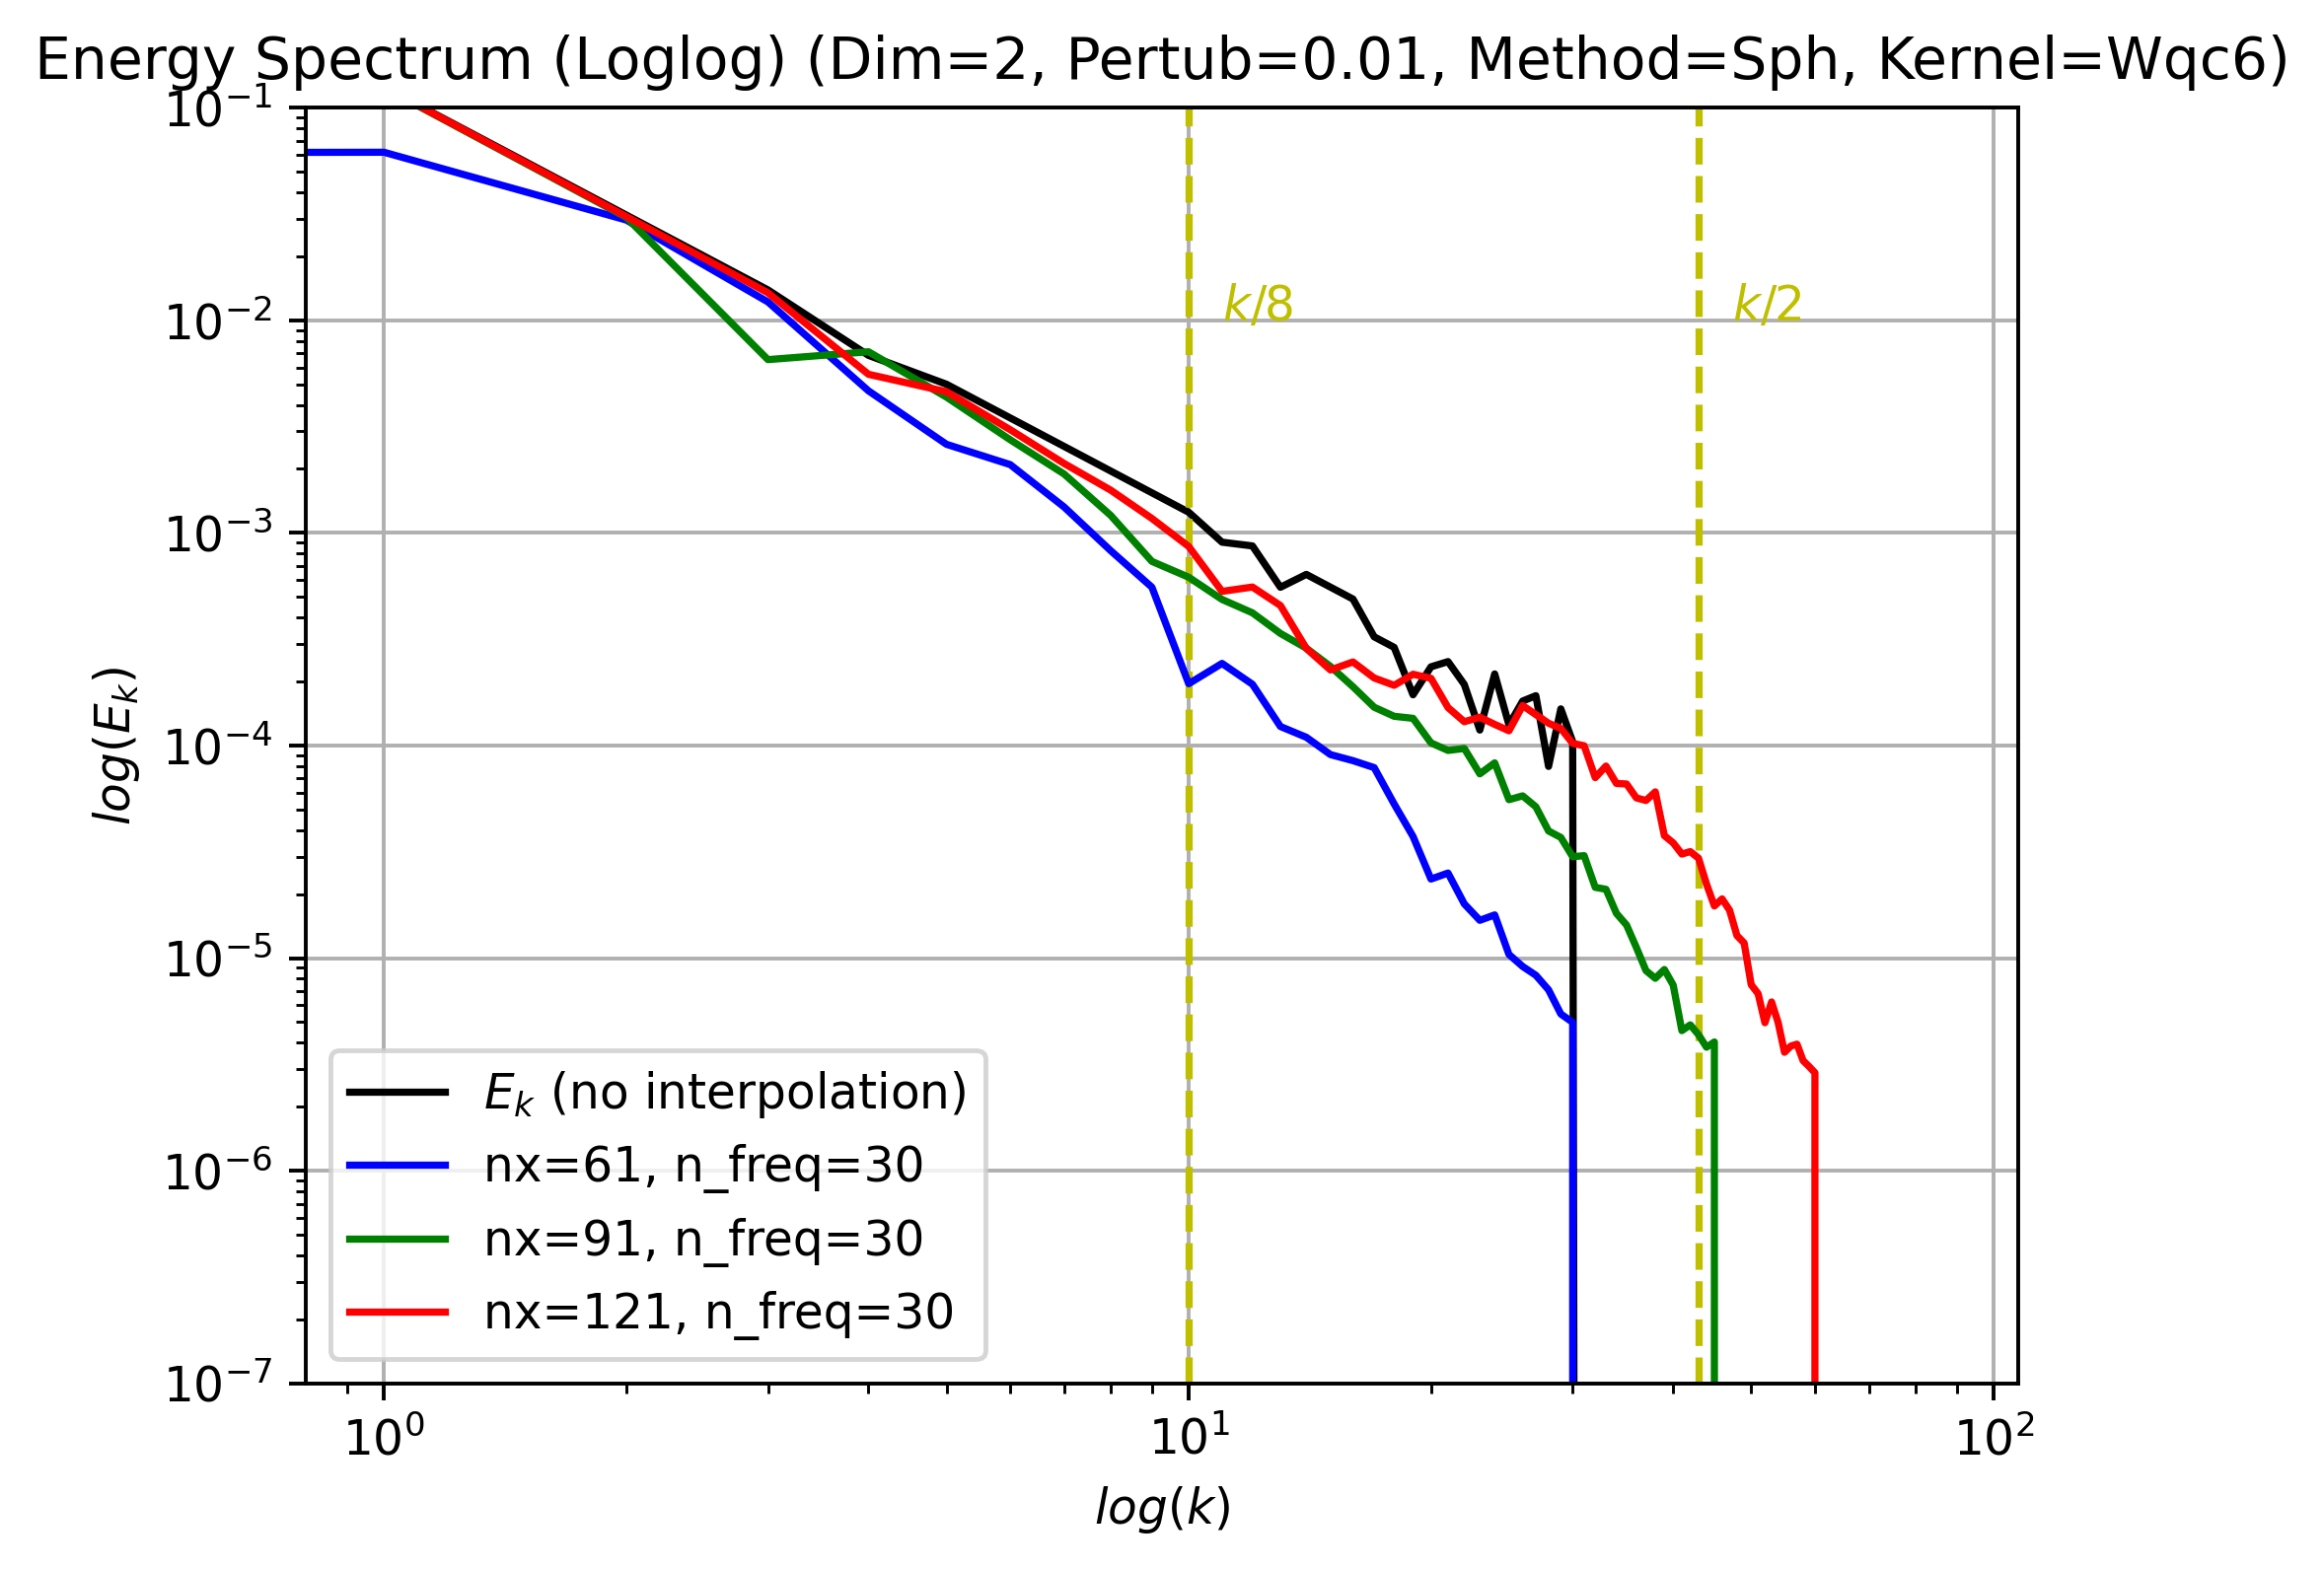
\includegraphics[width=6cm]{Code-Figures/sin-vel-prof-res/Energy Spectrum (Loglog) (Dim=2, Pertub=0.01, Method=Sph, Kernel=Wqc6).png}
		\caption{$2D$ $E(k)$ field}
	\end{subfigure}
	\begin{subfigure}{7cm}
		\centering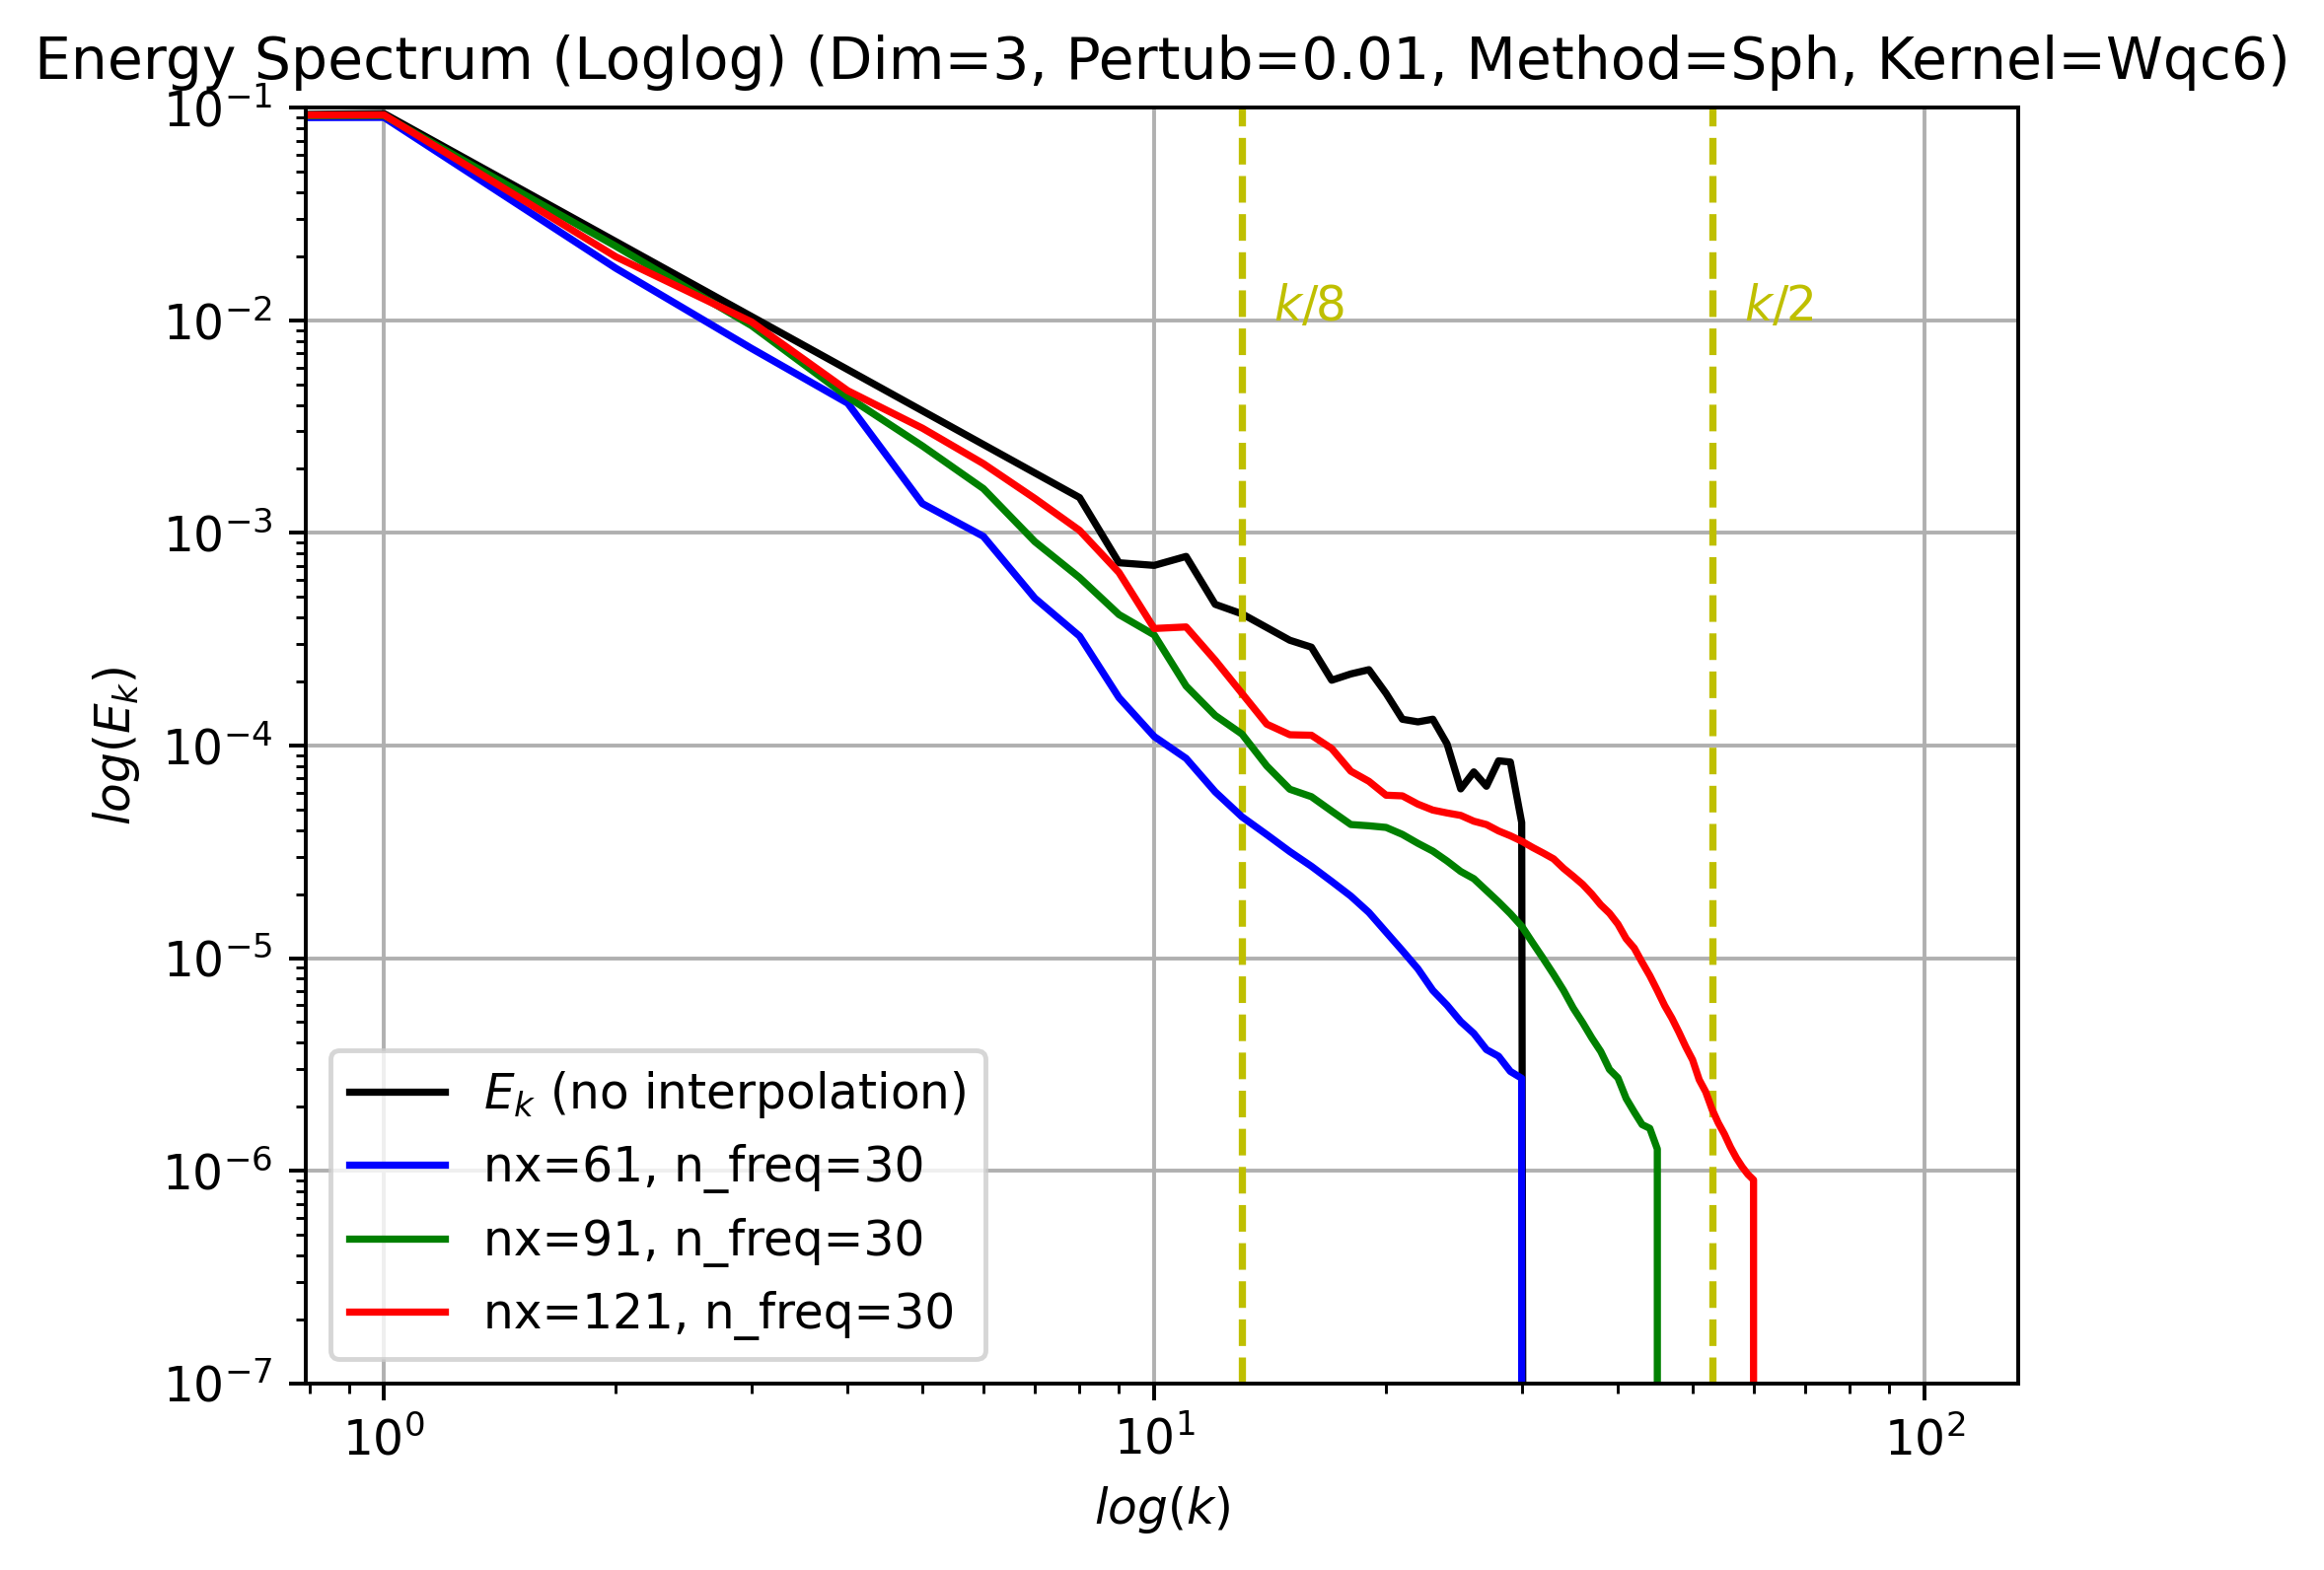
\includegraphics[width=6cm]{Code-Figures/sin-vel-prof-res/Energy Spectrum (Loglog) (Dim=3, Pertub=0.01, Method=Sph, Kernel=Wqc6).png}
		\caption{$3D$ $E(k)$ field}
	\end{subfigure}
	\caption{The scalar fields $E(k)$ for $1D$, $2D$, and $3D$ case, for various particle resolutions.}
	\label{fig:espec-scalar-fields-res}
\end{figure}


\subsection{Finite-time Lyapunov Exponent (FTLE) Field}

In order to compute the FTLE field, the flow field, at two different time instances, is required, i.e., $t_i$ and $t_f$.
The flow field corresponding to the earlier time instance is stored in the \texttt{initial} particle array, while the flow field corresponding to the later time instance is stored in the \texttt{final} particle array.

The forward-in-time (FIT) FTLE field is calculated as defined in the work of \cite{sun2016detection}:
\begin{equation}
	\lambda_{t_i}^{t_f}(\vect{x}) = \frac{1}{\abs{t_f - t_i}} \ln \bigg( \sqrt{\Lambda_{max}[ \mathbb{C}_{t_i}^{t_f}(\vect{x}) ]}  \bigg),
\end{equation}
\begin{equation}
  \mathbb{C}_{t_i}^{t_f}(\vect{x}) = \mathbb{F}_{t_i}^{t_f}(\vect{x})^T \mathbb{F}_{t_i}^{t_f}(\vect{x}),
\end{equation}
where, $\mathbb{F}_{t_i}^{t_f}(\vect{x})$ is the deformation gradient tensor, and $\Lambda_{max}$ is the maximum eigenvalue of the Cauchy-Green tensor $\mathbb{C}_{t_i}^{t_f}(\vect{x})$. Correspondingly, the backward-in-time (BIT) FTLE field is calculated as:
\begin{equation}
  \lambda_{t_f}^{t_i}(\vect{x}) = \frac{1}{\abs{t_f - t_i}} \ln \bigg( \sqrt{ \frac{1}{\Lambda_{min}[ \mathbb{C}_{t_i}^{t_f}(\vect{x}) ]} }  \bigg).
\end{equation}

The corresponding SPH approximations for the above equations are:
\begin{equation}
  \mathbb{F}_{t_i}^{t_f}(\vect{x}_i) = \sum_{j} \frac{m_j}{\rho_j} \vect{X}_{ji} \otimes \nabla \mathbb{L}( \vect{x}_i ) \DWIJ,
\end{equation}
\begin{equation}
  \mathbb{L}( \vect{x}_i ) = \bigg[ \sum_j \vect{x}_{ji} \otimes \nabla_i W(\abs{\vect{X}_{ji}}, h_i) \bigg]^{-1},
\end{equation}
where $(\vect{x}_i, \vect{X}_i)$ corresponds to the initial and final position of the same particle.

In order to test the correctness of the FTLE field computation, the following test cases were devised.
\begin{itemize}
  \item \texttt{parabolic}
  \begin{equation}
    X = 1.5x, \quad Y = x^2 + y,
  \end{equation}

  \item \texttt{spiral}
  \begin{equation}
    X = x + 0.1 \cos(2 \pi r^2), \quad Y = y + 0.1 \sin(2 \pi r^2), \quad r = \sqrt{x^2 + y^2},
    \end{equation}
\end{itemize}

\begin{figure}[htbp!]
		\centering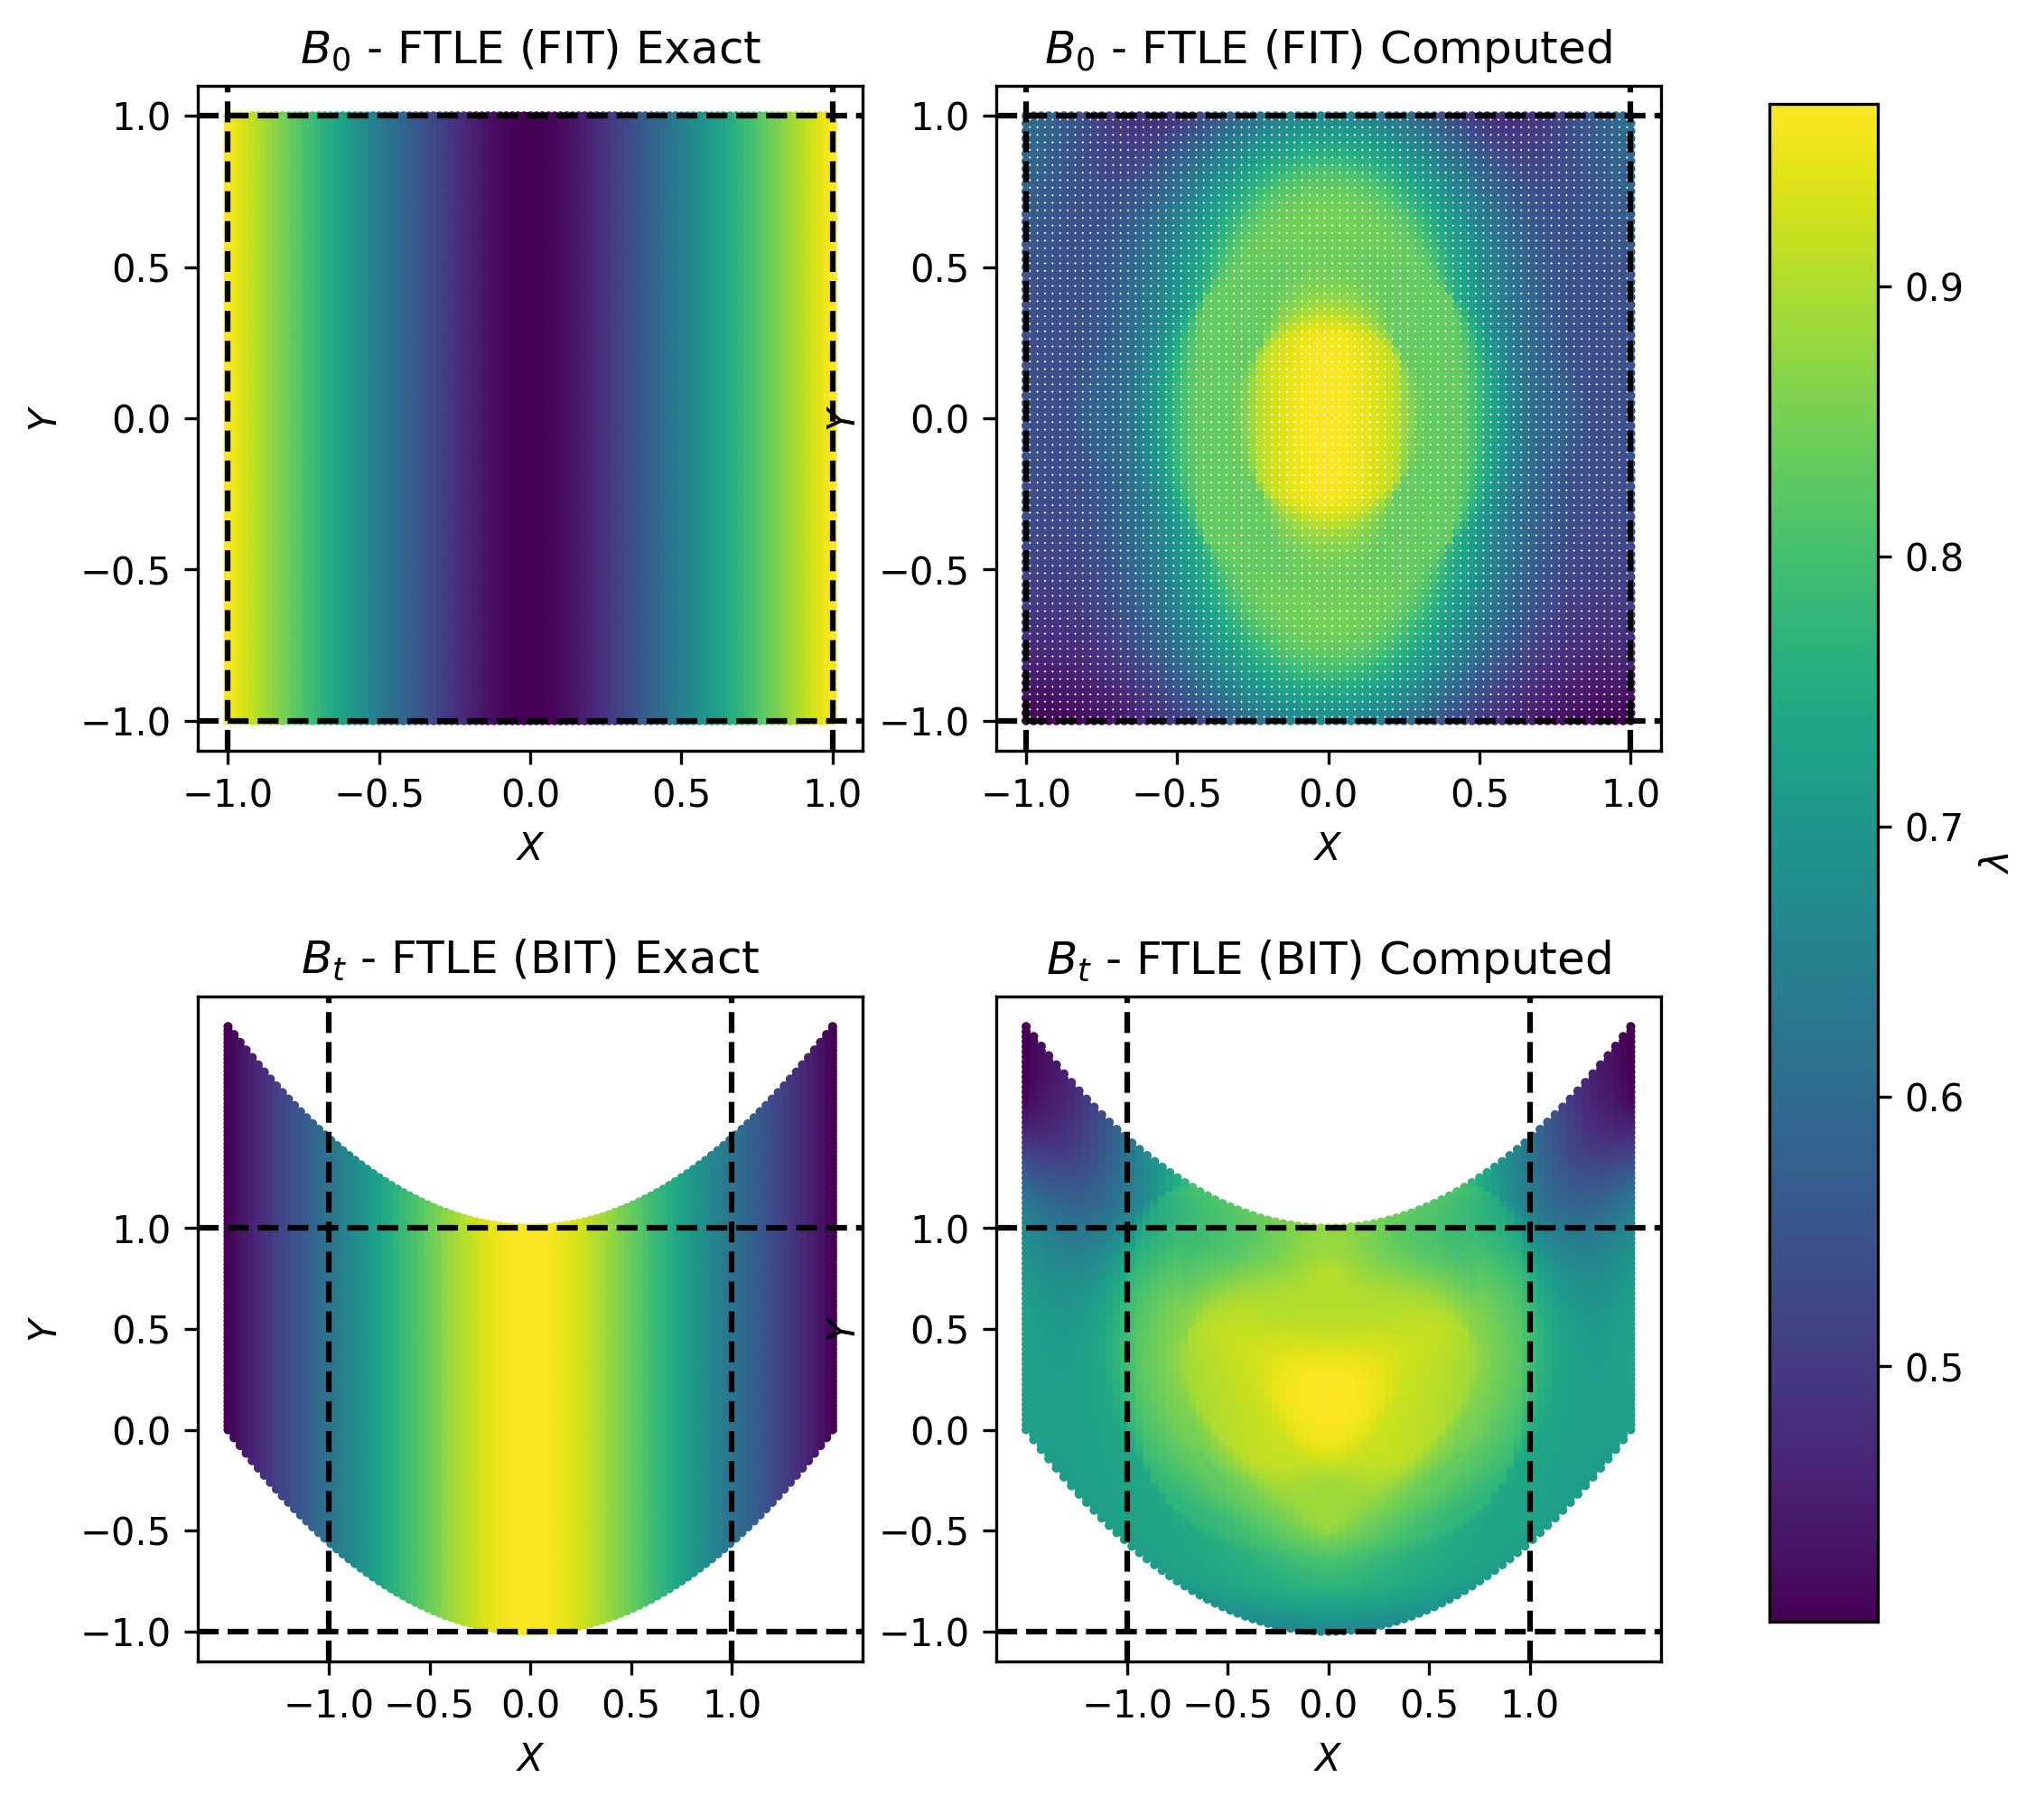
\includegraphics[width=10cm]{Code-Figures/ftle_parabolic.png}
		\caption{Parabolic displacement field}
    \label{fig:ftle-parabolic}
\end{figure}
\begin{figure}[htbp!]
  \centering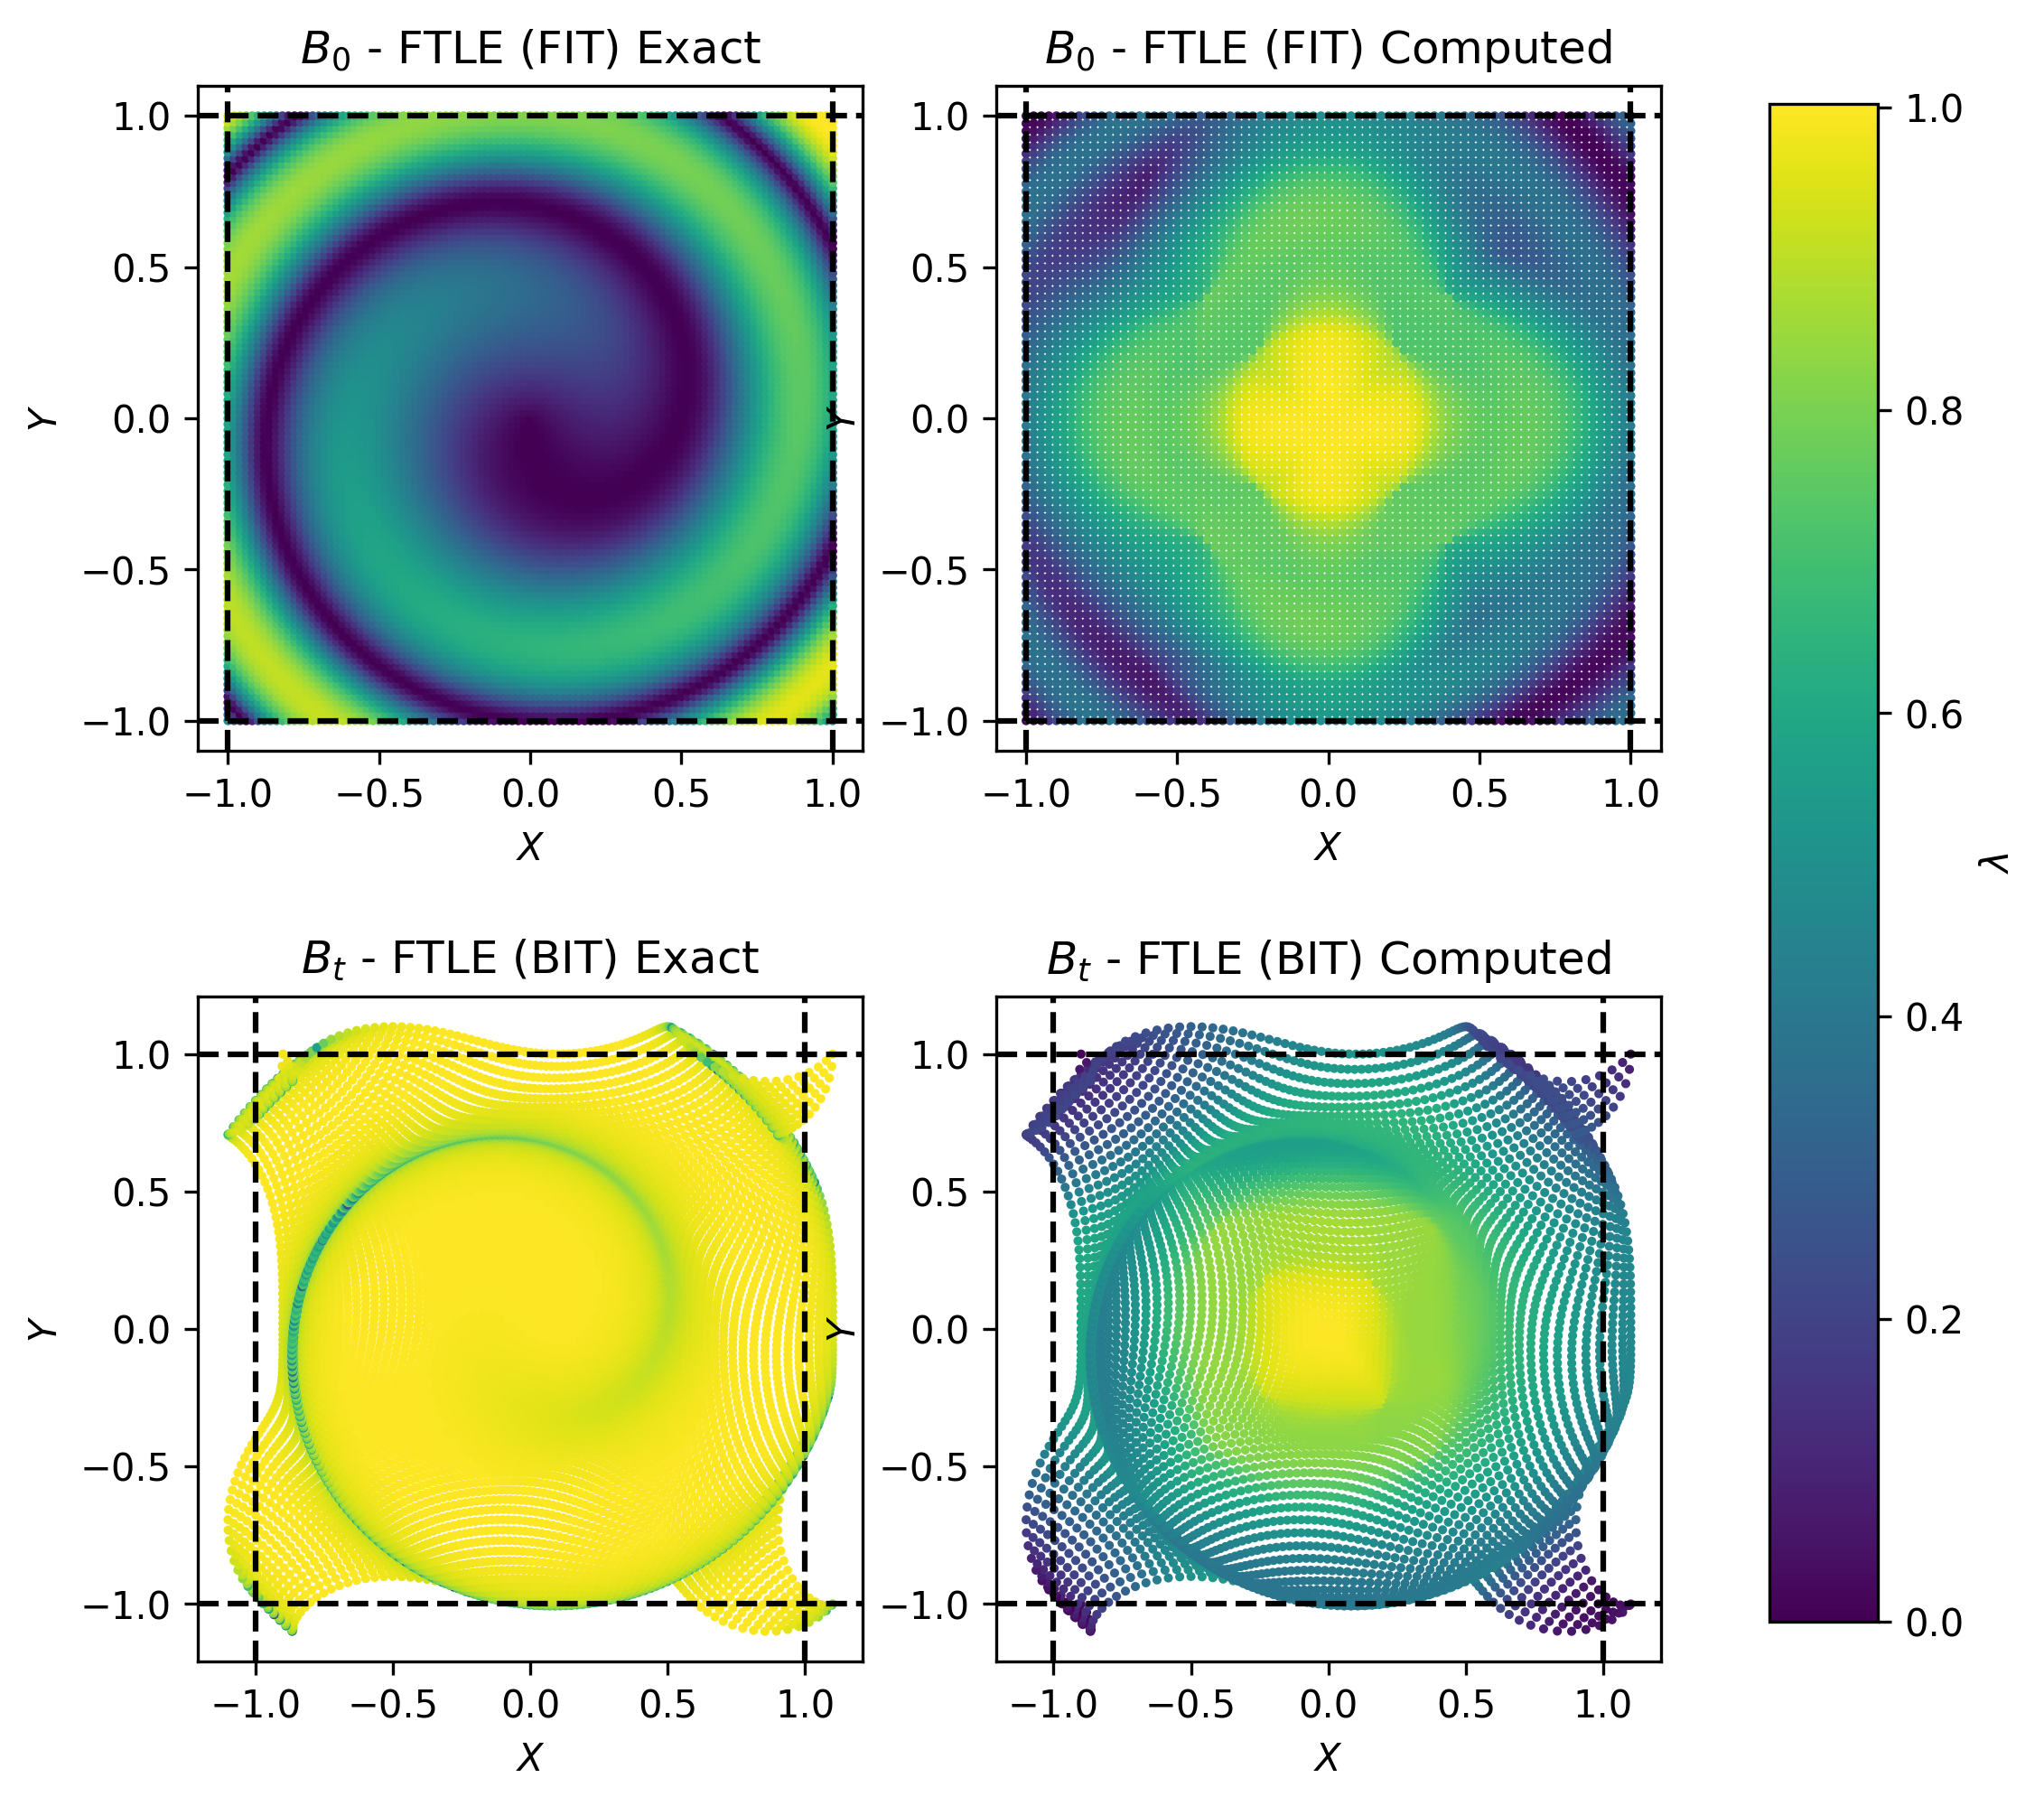
\includegraphics[width=10cm]{Code-Figures/ftle_spiral.png}
  \caption{Spiral displacement field}
  \label{fig:ftle-spiral}
\end{figure}

As seen in \figref{fig:ftle-parabolic} and \figref{fig:ftle-spiral} ($B_0$: initial configuration, $B_t$: final configuration), it can be observed that although the FTLE field is capable of qualitatively capturing the evolution of the configurations, i.e., attracting/repelling pathlines, it is however, not as accurate in terms of actually capturing the exact pathlines. Therefore, it was concluded that in place of FTLE fields, tracer particles could be used to visualise the flow field, which would be more accurate in terms of capturing the exact pathlines but would be computationally more expensive since the tracer particles would have to be advected along with the flow field, and would also require additional post-processing to visualise the pathlines. They would also have to be done in situ, i.e., during the simulation itself, as opposed to the FTLE fields, which can be computed post-simulation or in situ.
% TODO: iPad fig of attracting and repelling pathlines


\section{Turbulence Modelling}
\subsection{Implementation of models}
A broad classification of the major categories of turbulence models has already been discussed in \chapref{chap:turbulence-modelling}.
In order to better understand the nature of each major category and to subsequently understand the implementation of the same, a select few representative schemes from each of these models are considered, which are listed in \tabref{tab:rep-turb-models}.

\begin{table}[htbp!]
  \centering
  \resizebox{\textwidth}{!}{%
  \begin{tabular}{|l|l|l|l|}
  \hline
  \multicolumn{1}{|c|}{\textbf{Turbulence Model}} & \multicolumn{1}{c|}{\textbf{Review Section}} & \multicolumn{1}{c|}{\textbf{Scheme Name}}                                                                               & \multicolumn{1}{c|}{\textbf{Reference}}  \\ \hline
  Viscosity-based Model                           & \secref{sec:visc-based-model}                  & \begin{tabular}[c]{@{}l@{}}Lagrangian with iterative PST and \texttt{coupled\_c} viscosity formulation\\ (L-IPST-C)\end{tabular} & \cite{Negi2022Techniques}            \\ \hline
  Large Eddy Simulation-based Model               & \secref{sec:les-based-model}                   & SPH-LES                                                                                                                          & \cite{Okraschevski2022}              \\ \hline
  Lagrangian LES-based Model                      & \secref{sec:lagrangian-les-based-model}        & $\delta$-LES-SPH                                                                                                                 & \cite{Colagrossi2021QuasiLagrangian} \\ \hline
  RANS-based k-epsilon Model                      & \secref{sec:rans-based-k-epsilon-model}        & $k-\epsilon$ SPH                                                                                                                 & \cite{Shao2006}                      \\ \hline
  LANS-based Model                                & \secref{sec:lans-based-model}                  & SPH-$\epsilon$                                                                                                                   & \cite{Monaghan2017}                  \\ \hline
  \end{tabular}%
  }
  \caption{Implementation of representative turbulence models.}
  \label{tab:rep-turb-models}
\end{table}

In order to test the schemes for SOC, the Taylor-Green vortex (TGV) problem is chosen. The test cases are coded using \texttt{automan} \parencite{RamachandranAutoman2018}, an open-source, Python-based automation framework. All of the simulations run hereafter are run upto a final time of $t_f=0.1$, with the resolution for each run consisting of $N=[25^2, 50^2, 100^2]$ particles respectively, with the Reynolds number ranging between $Re=[100, 1000, 10000]$ respectively. All simulations are run using the \texttt{WendlandQuinticC4} kernel, with a radius multiplier of $2.0$. This choice was based on the work of \cite{Negi2022Techniques}.

The $L_1$ error for each simulation in a run is computed and plotted against the particle spacing inverse to evaluate the scheme's order of convergence (OOC). The $L_1$ error at a given time instance is computed as:
\begin{equation}
  L_1(t) = \frac{mean{\abs{\vect{v}^2(t) - \vect{v}^2_{exact}(t)}}}{mean{\abs{\vect{v}^2_{exact}(t)}}},
\end{equation}
where, $\vect{v}(t)$ is the velocity field at time $t$, and $\vect{v}_{exact}(t)$ is the exact velocity field at time $t$.
Subsequently, the $L_1$ error for the entire simulation is defined as the mean over all the time instances, i.e.,
\begin{equation}
  L_1 = \frac{1}{n_t} \sum_{i=1}^{n_t} L_1(t_i).
\end{equation}

\subsection{L-IPST-C Scheme}

The L-IPST-C scheme was considered over the other viscosity-based schemes since it was observed to be second-order convergent (SOC) by \cite{Negi2022Techniques}, for a wide variety of problems, which included the Gresho vortex problem, Kelvin-Helmholtz instability problem, and the Taylor-Green vortex problem. This scheme considers the weakly-compressible NS equations the governing equations and uses the \texttt{coupled\_c} viscosity formulation, which is corrected using the Bonet and Lok correction \parencite{bonet1999variational}. Hence, since the scheme, by definition, has the viscous term in its governing equation, it does require any additional `artificial'-viscosity term to be added.
The scheme also incorporates the iterative particle shifting technique (IPST) by \cite{Huang_Long_Li_Liu_2019} in order to redistribute the particles to obtain a reasonably uniform grid of particles in the domain. Besides shifting the position of the particles, the scheme also updates the particles' properties, such as the density and velocity, to keep the approximation of the particle $O(h^2)$.
Based on the parametric study conducted by \cite{Negi2022Techniques}, the proposed scheme is observed to be SOC by considering the speed of sound to be $c_s = 20$ and the shifting frequency for the particles through PST to be at every ten iterations $f_{pst} = 10$.

Since the study dealt with problems of low $Re$, the scheme was tested for various time integrators from the Runge-Kutta family of integrators to identify their effects and the most suitable integrator for problems of high $Re$.
The integrators considered were:
\begin{itemize}
  \item Predict-Evaluate-Correct (\texttt{PEC}),
  \item Runge-Kutta 2 (\texttt{RK2}),
  \item Runge-Kutta 2 with adaptive time-step (\texttt{RK2 Adaptive}),
  \item Runge-Kutta 3 (\texttt{RK3}), and
  \item Runge-Kutta 4 (\texttt{RK4}),
\end{itemize}
with a corresponding $CFL$ values of $[1, 1, 1.5, 2, 2]$ respectively.

\begin{figure}[htbp!]
  \begin{subfigure}{7cm}
    \centering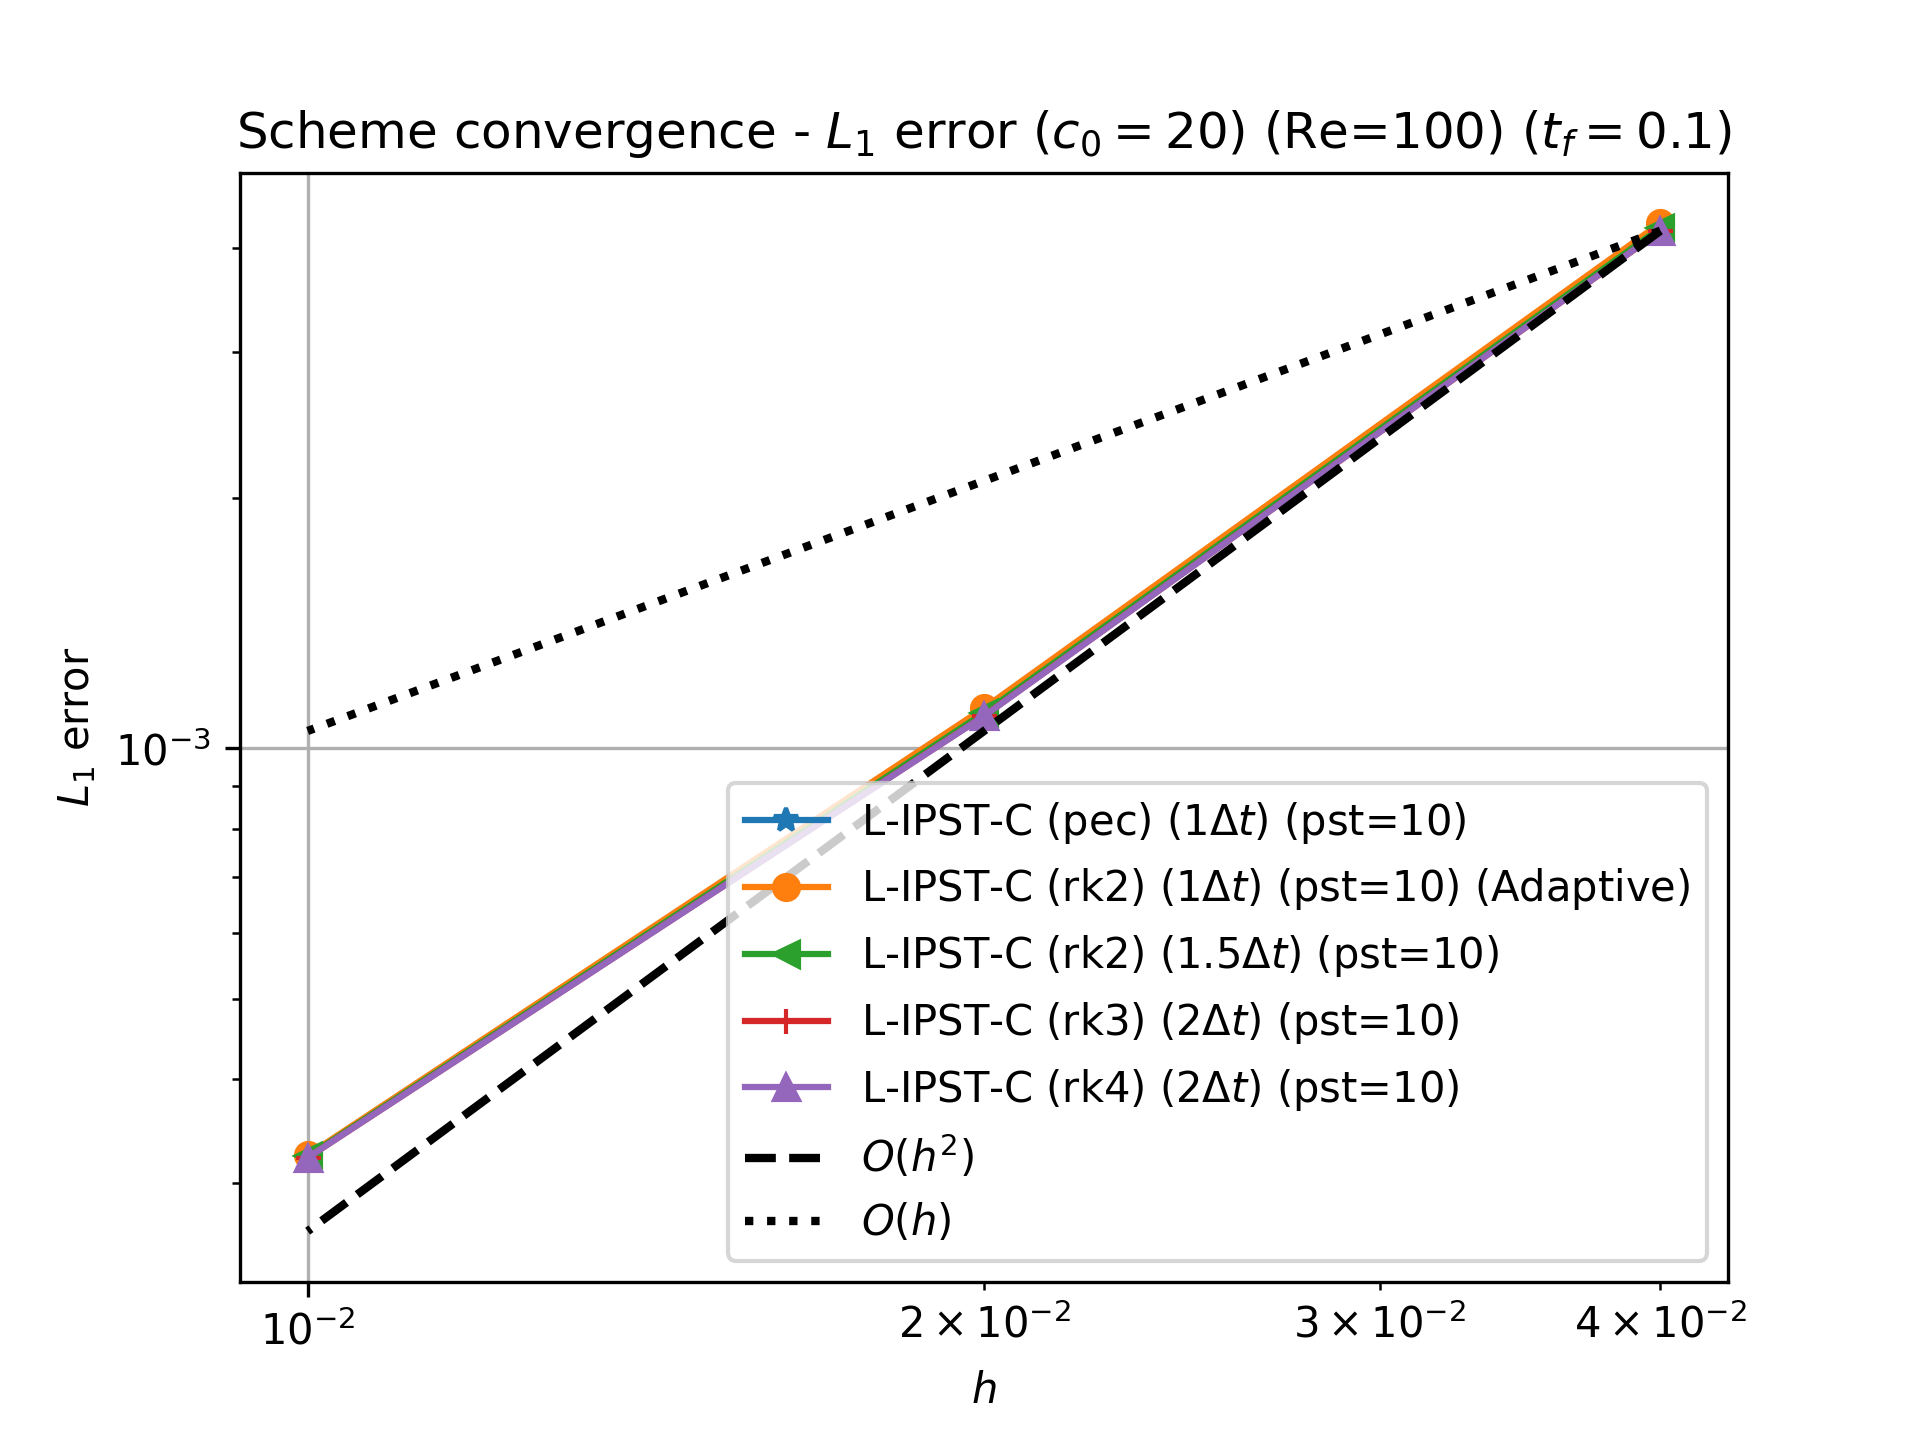
\includegraphics[width=6cm]{Code-Figures/lipstc/integrator/dt_pois_conv_c0_20_re_100.png}
    \caption{$Re = 100$}
  \end{subfigure}
  \begin{subfigure}{7cm}
    \centering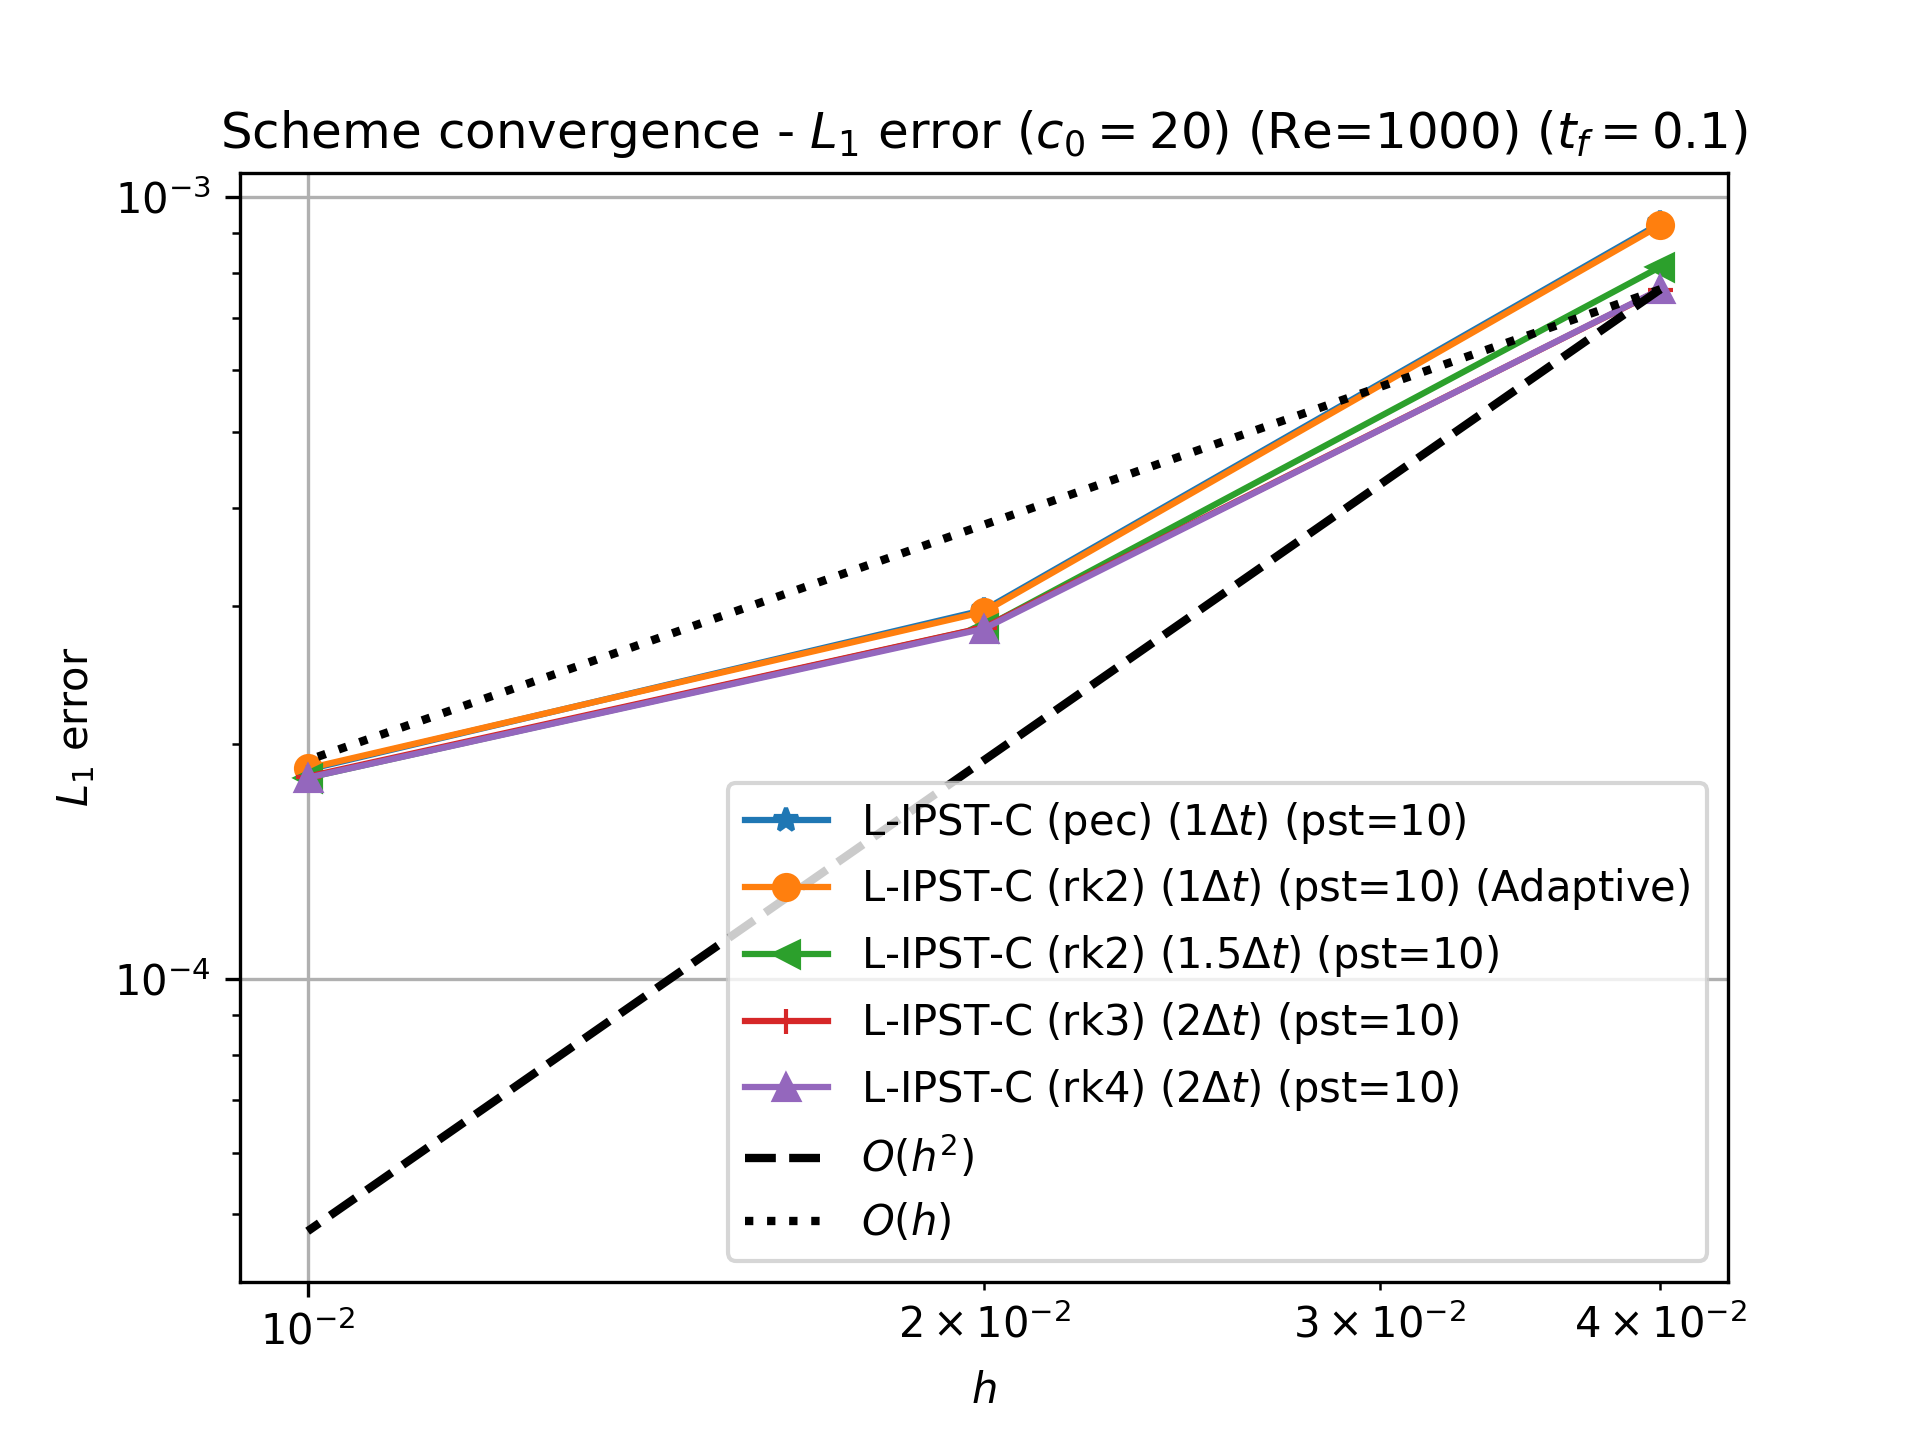
\includegraphics[width=6cm]{Code-Figures/lipstc/integrator/dt_pois_conv_c0_20_re_1000.png}
    \caption{$Re = 1000$}
  \end{subfigure}
  \begin{subfigure}{7cm}
    \centering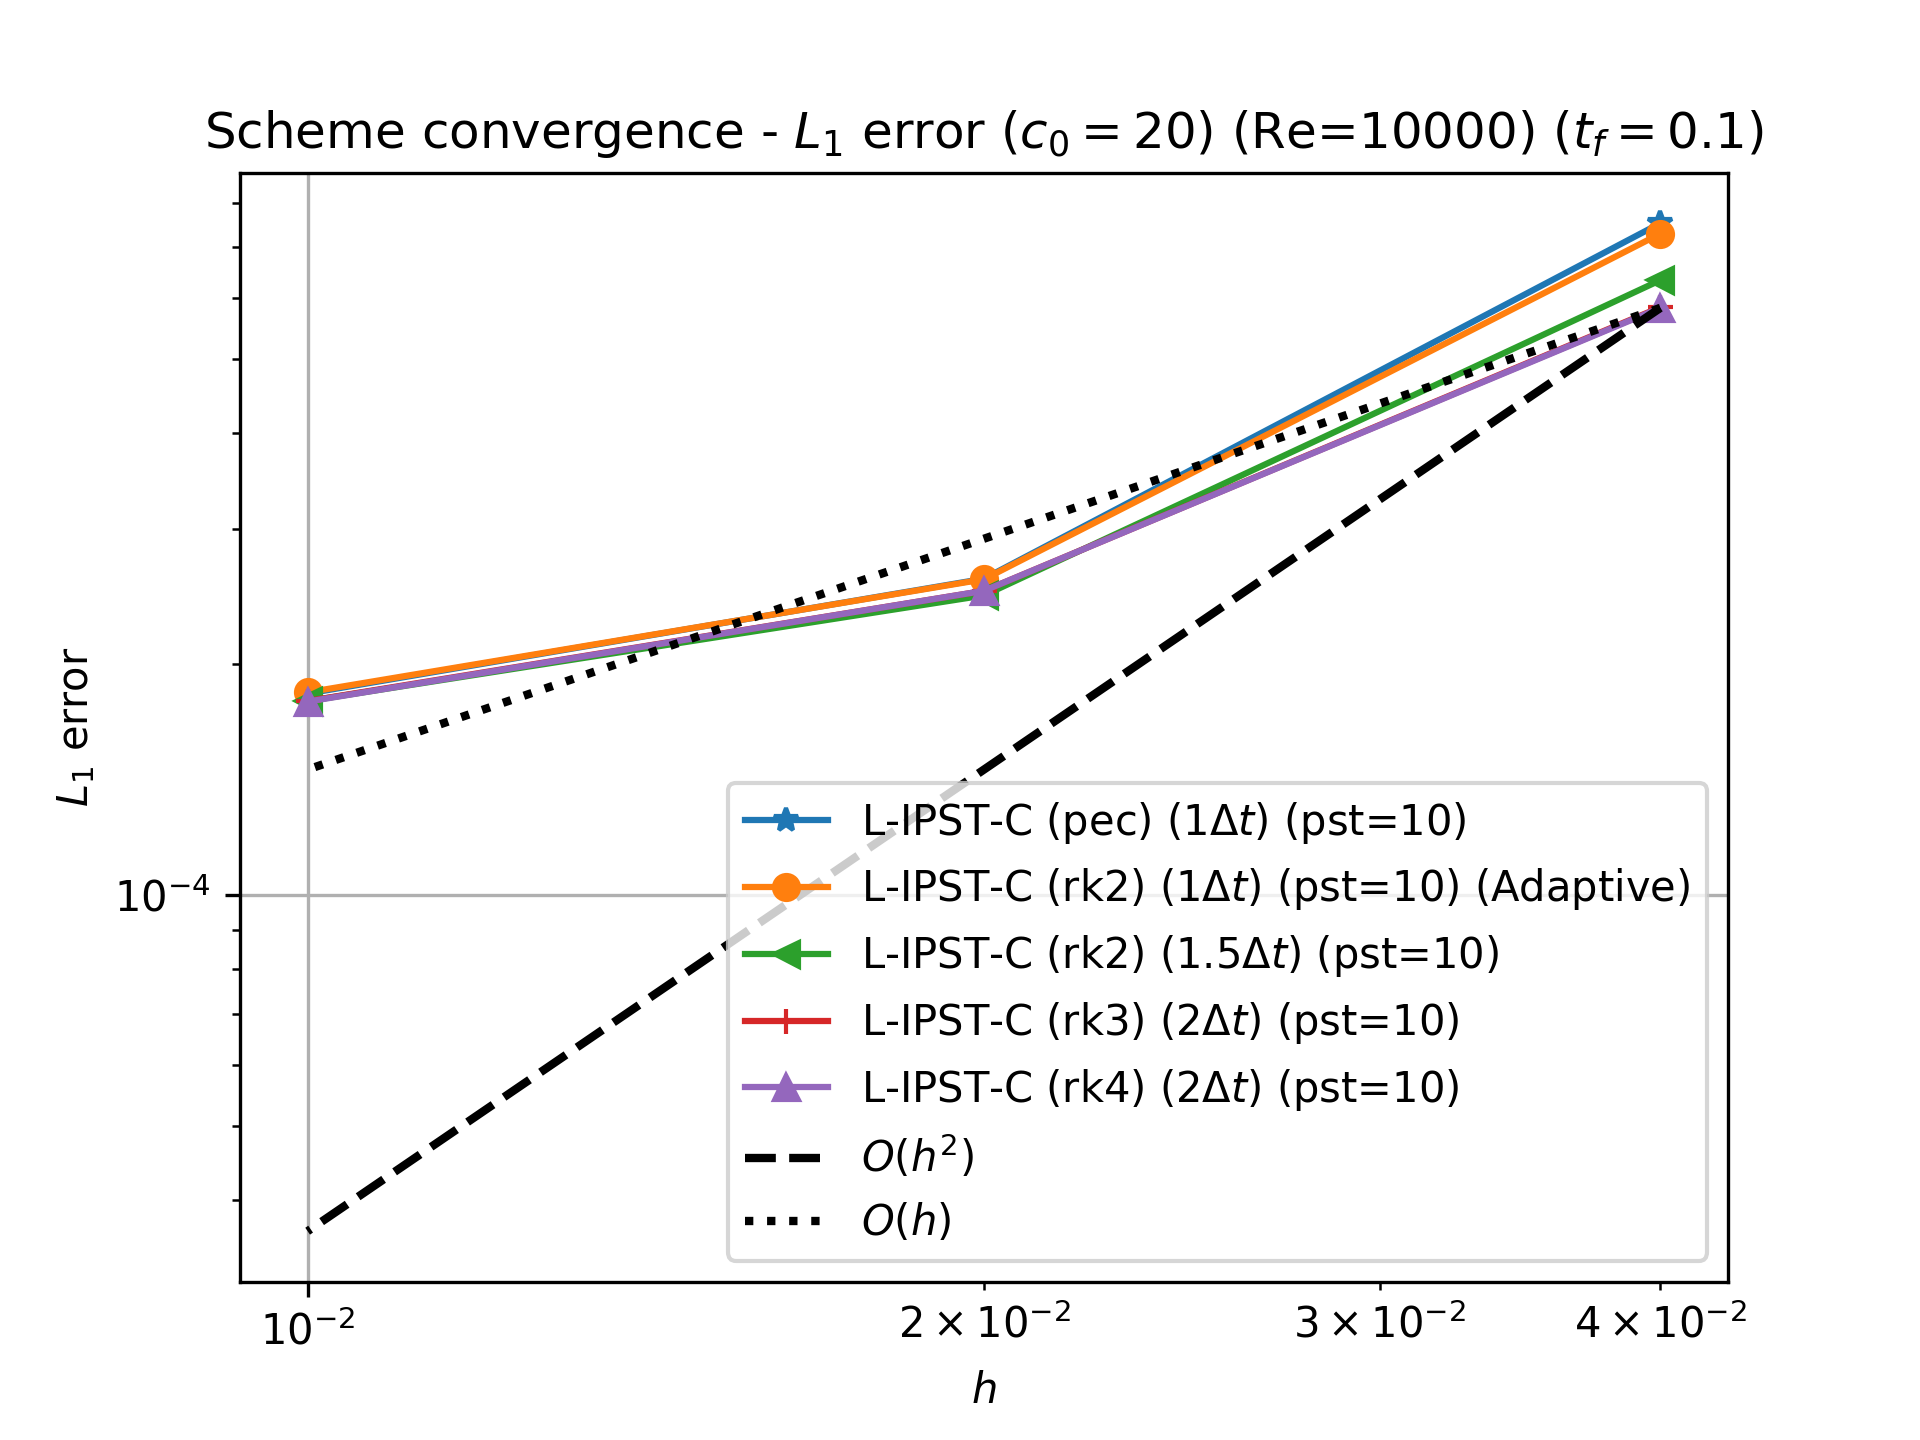
\includegraphics[width=6cm]{Code-Figures/lipstc/integrator/dt_pois_conv_c0_20_re_10000.png}
    \caption{$Re = 10000$}
  \end{subfigure}
  \caption{Convergence of the L-IPST-C scheme for various time-integrators.}
  \label{fig:lipstc-integrator}
\end{figure}

From the results shown in \figref{fig:lipstc-integrator}, it is evident that the order of the integrator does not appear to have much effect on the OOC and almost negligible effect on the actual magnitude of the $L_1$ errors as well.
This highlights a much more important aspect of the effect and role of time integrators in SPH: the time-step size is the most critical factor. The order of the integrator is less important since the time-step size is typically chosen to be small enough to ensure stability. Hence, the error introduced by the time integrator is typically negligible.

Also, when the run-times of these integrators were analysed, the higher order integrators were observed to be more computationally expensive, allowing for the \texttt{PEC} integrator to be around $\approx 1.6\times$ faster, which is reflected in the run-times shown in \figref{fig:lipstc-integrator-rt}.
Typically, such higher-order integrators can be used with much larger $CFL$ values, allowing for larger time steps and faster run times. However, in the case of SPH, such generalisations cannot be made since the stability of the scheme is not only dependent on the time-step size but also on the particle spacing, and hence, the $CFL$ value is typically chosen to be close to $1.0-2.0$.
Therefore, the \texttt{PEC} integrator is chosen as the default integrator for the L-IPST-C scheme.

\begin{figure}[htbp!]
  \begin{subfigure}{7cm}
    \centering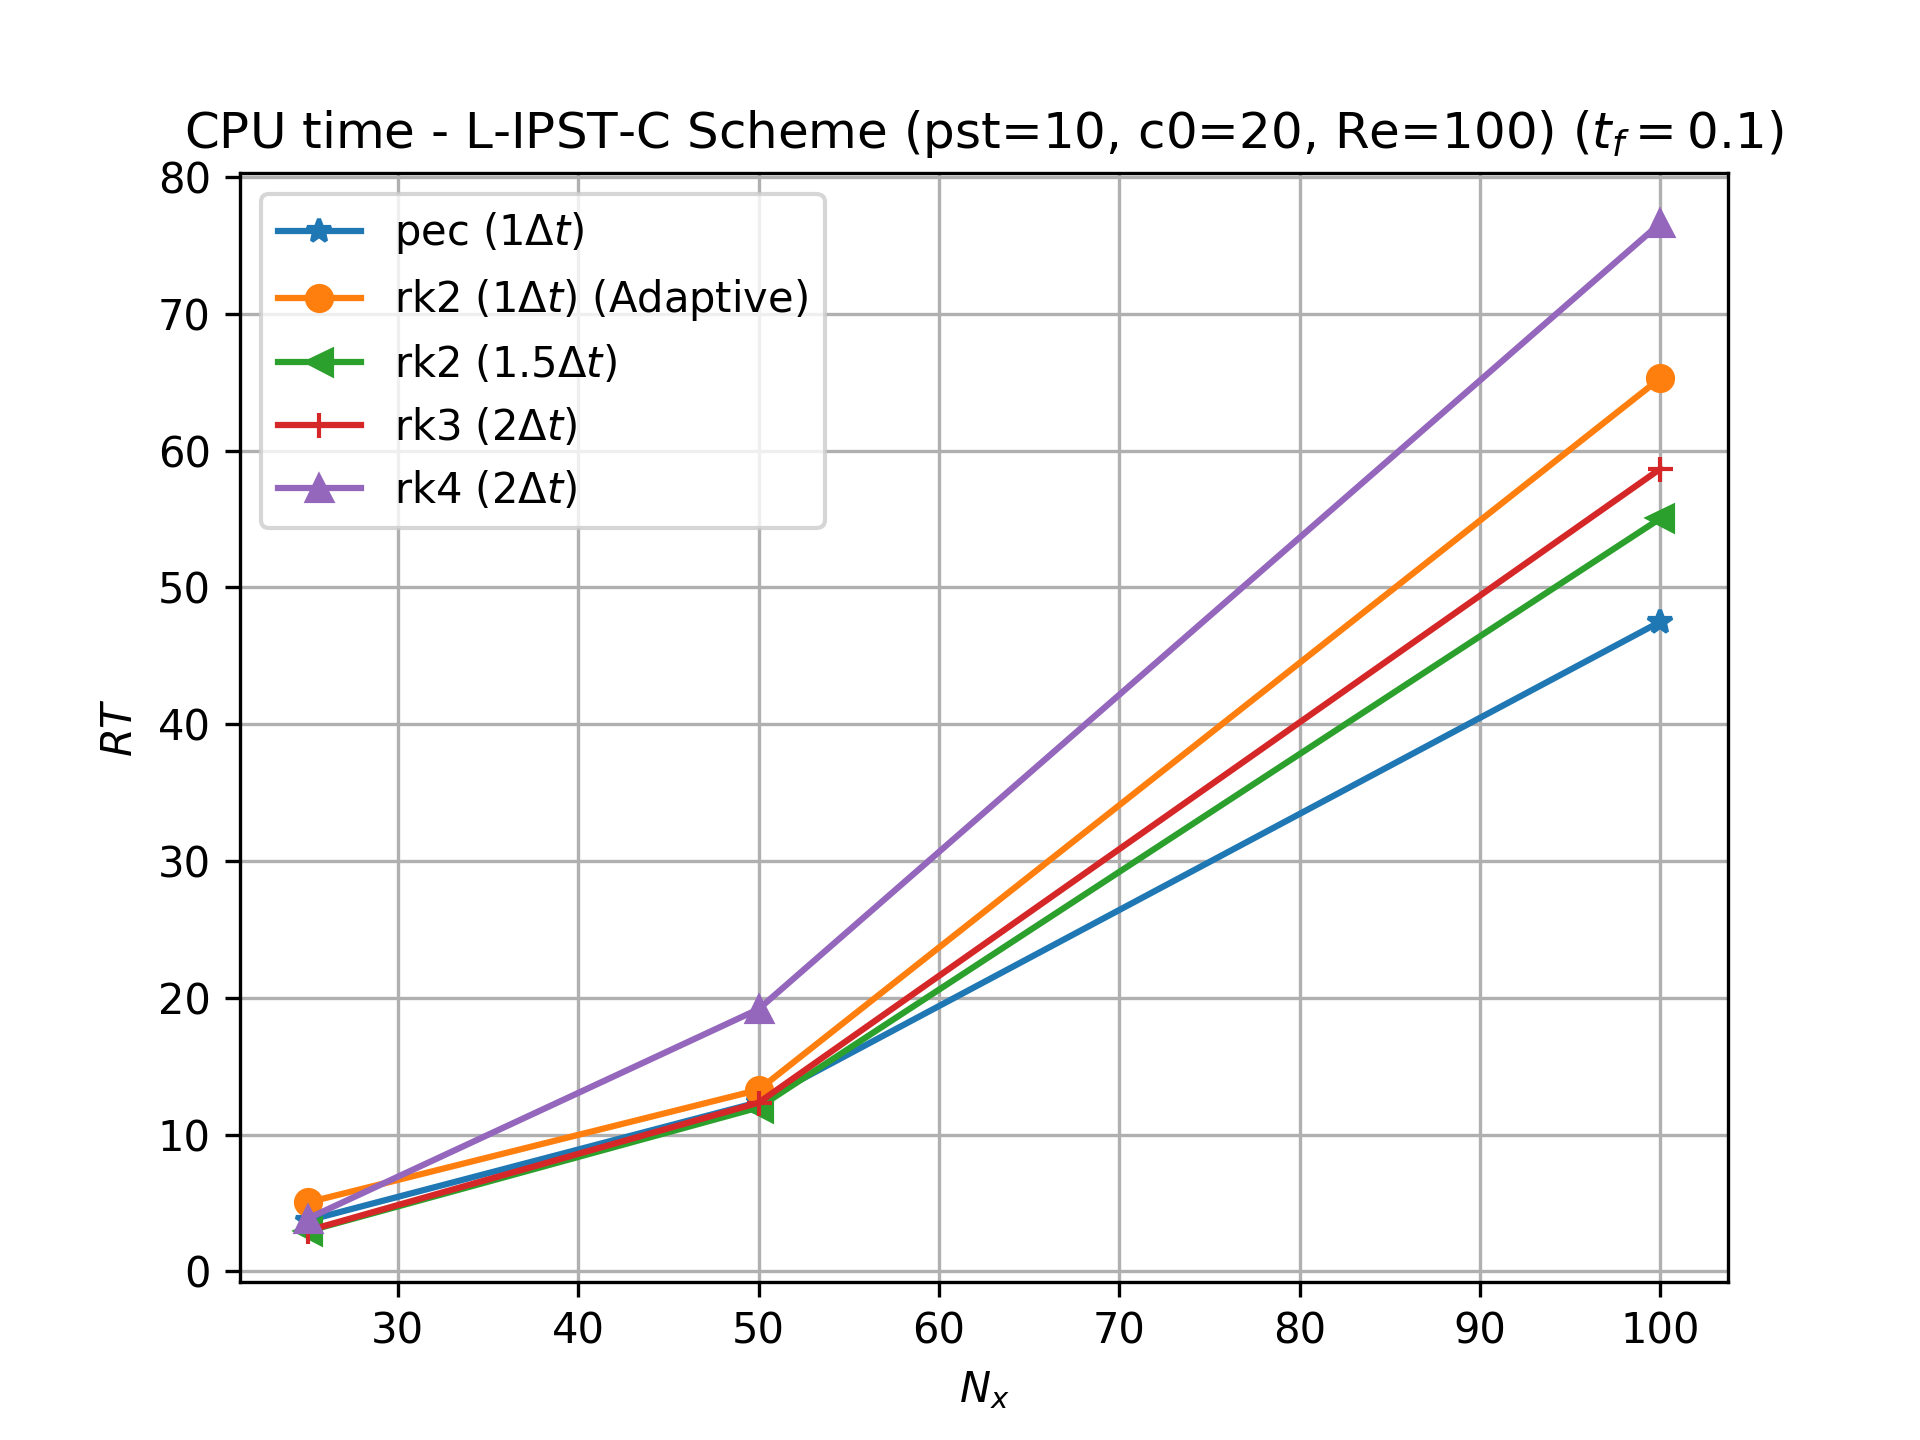
\includegraphics[width=6cm]{Code-Figures/lipstc/integrator/pois_rt_pst_10_c0_20_re_100.png}
    \caption{$Re = 100$}
  \end{subfigure}
  \begin{subfigure}{7cm}
    \centering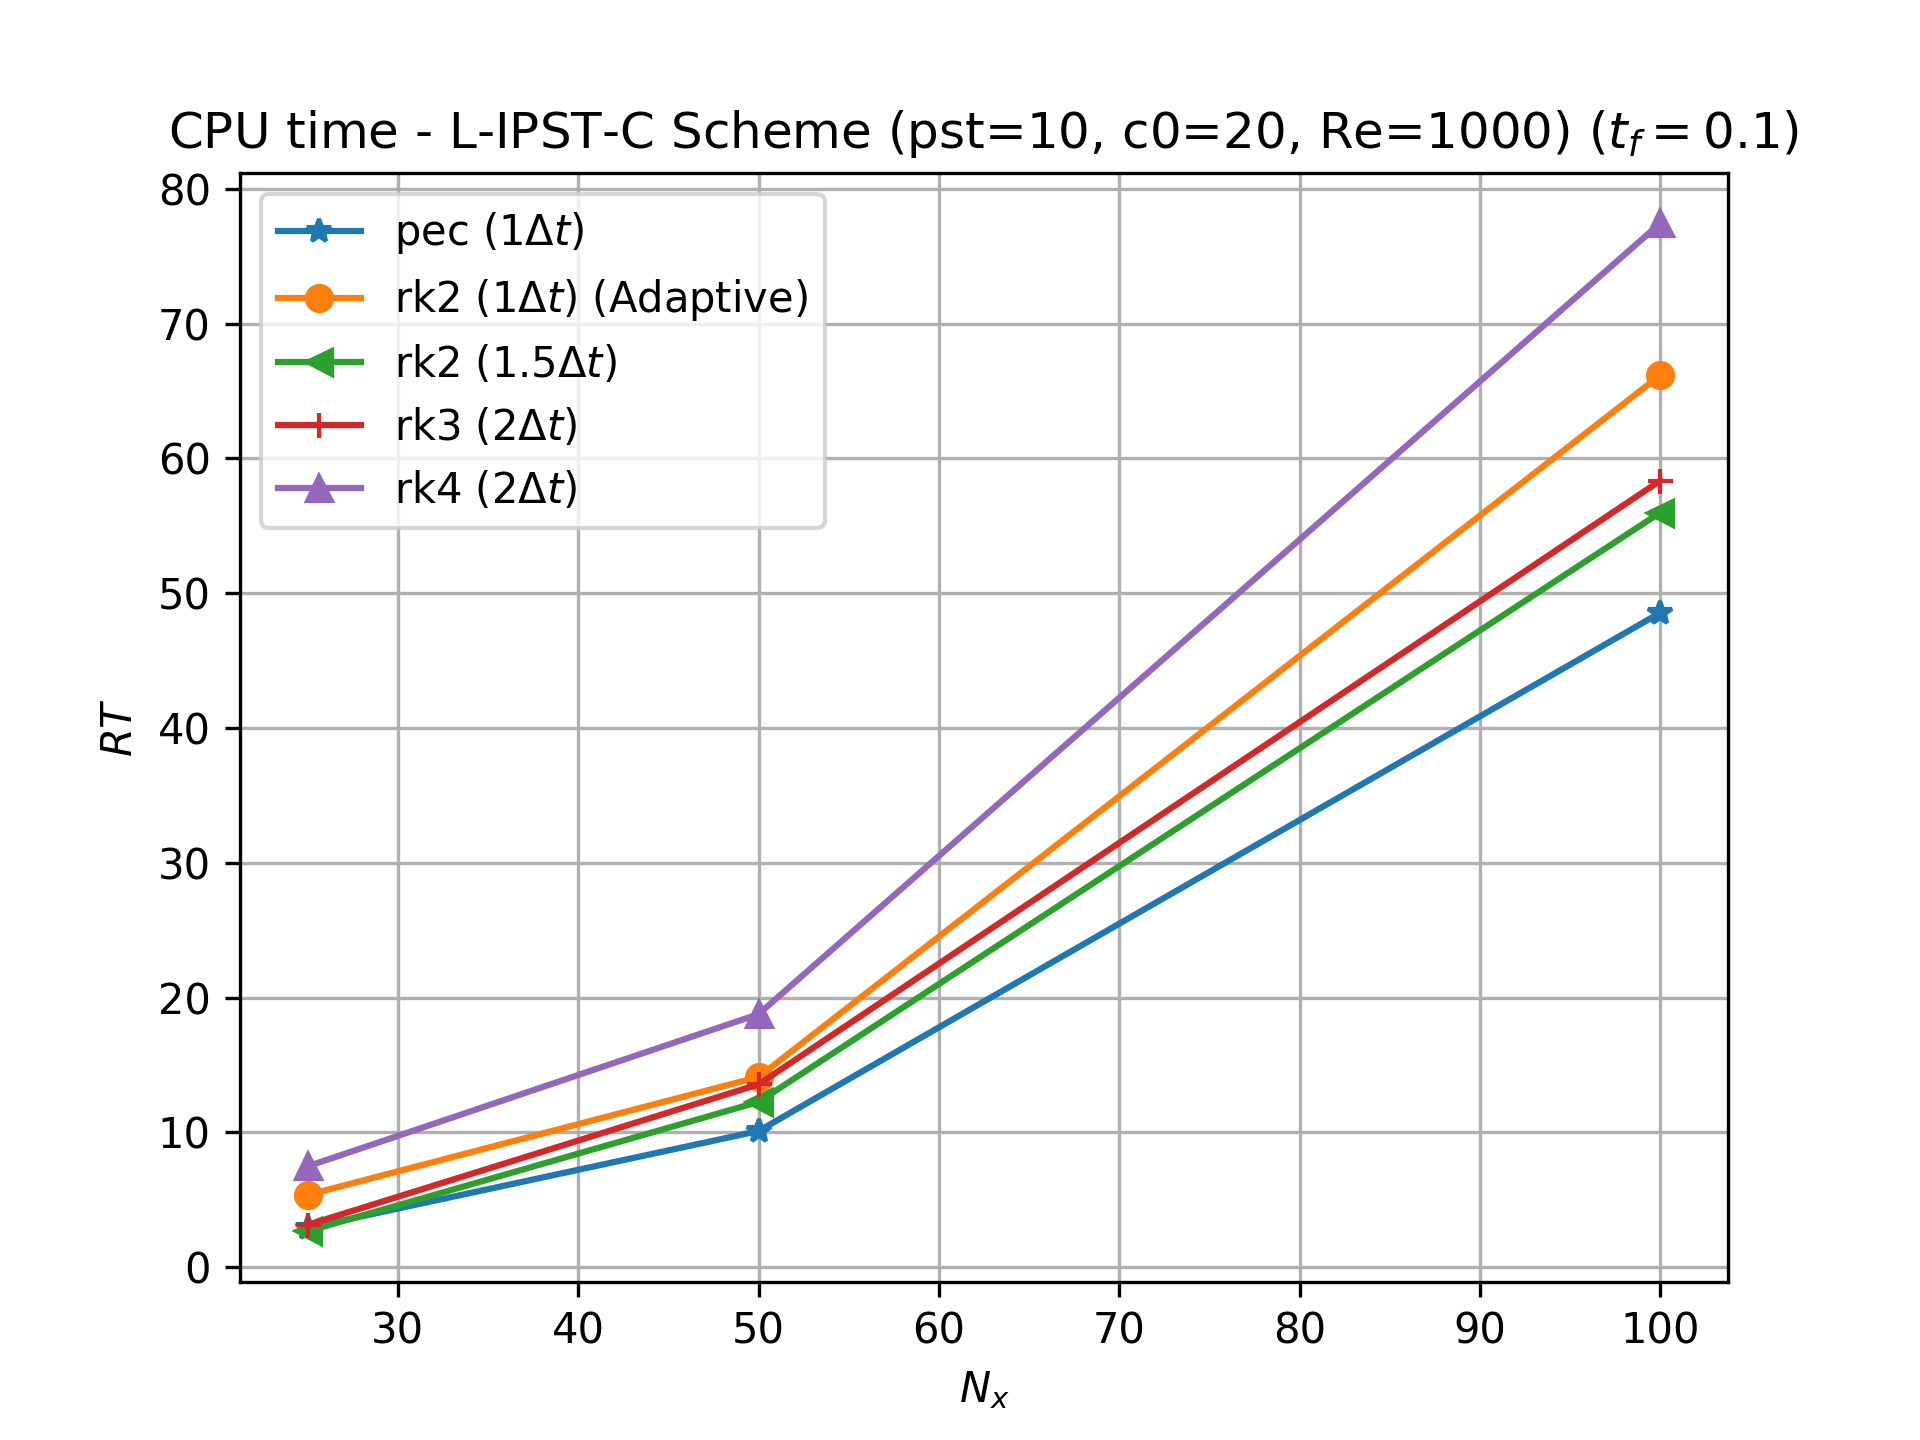
\includegraphics[width=6cm]{Code-Figures/lipstc/integrator/pois_rt_pst_10_c0_20_re_1000.png}
    \caption{$Re = 1000$}
  \end{subfigure}
  \begin{subfigure}{7cm}
    \centering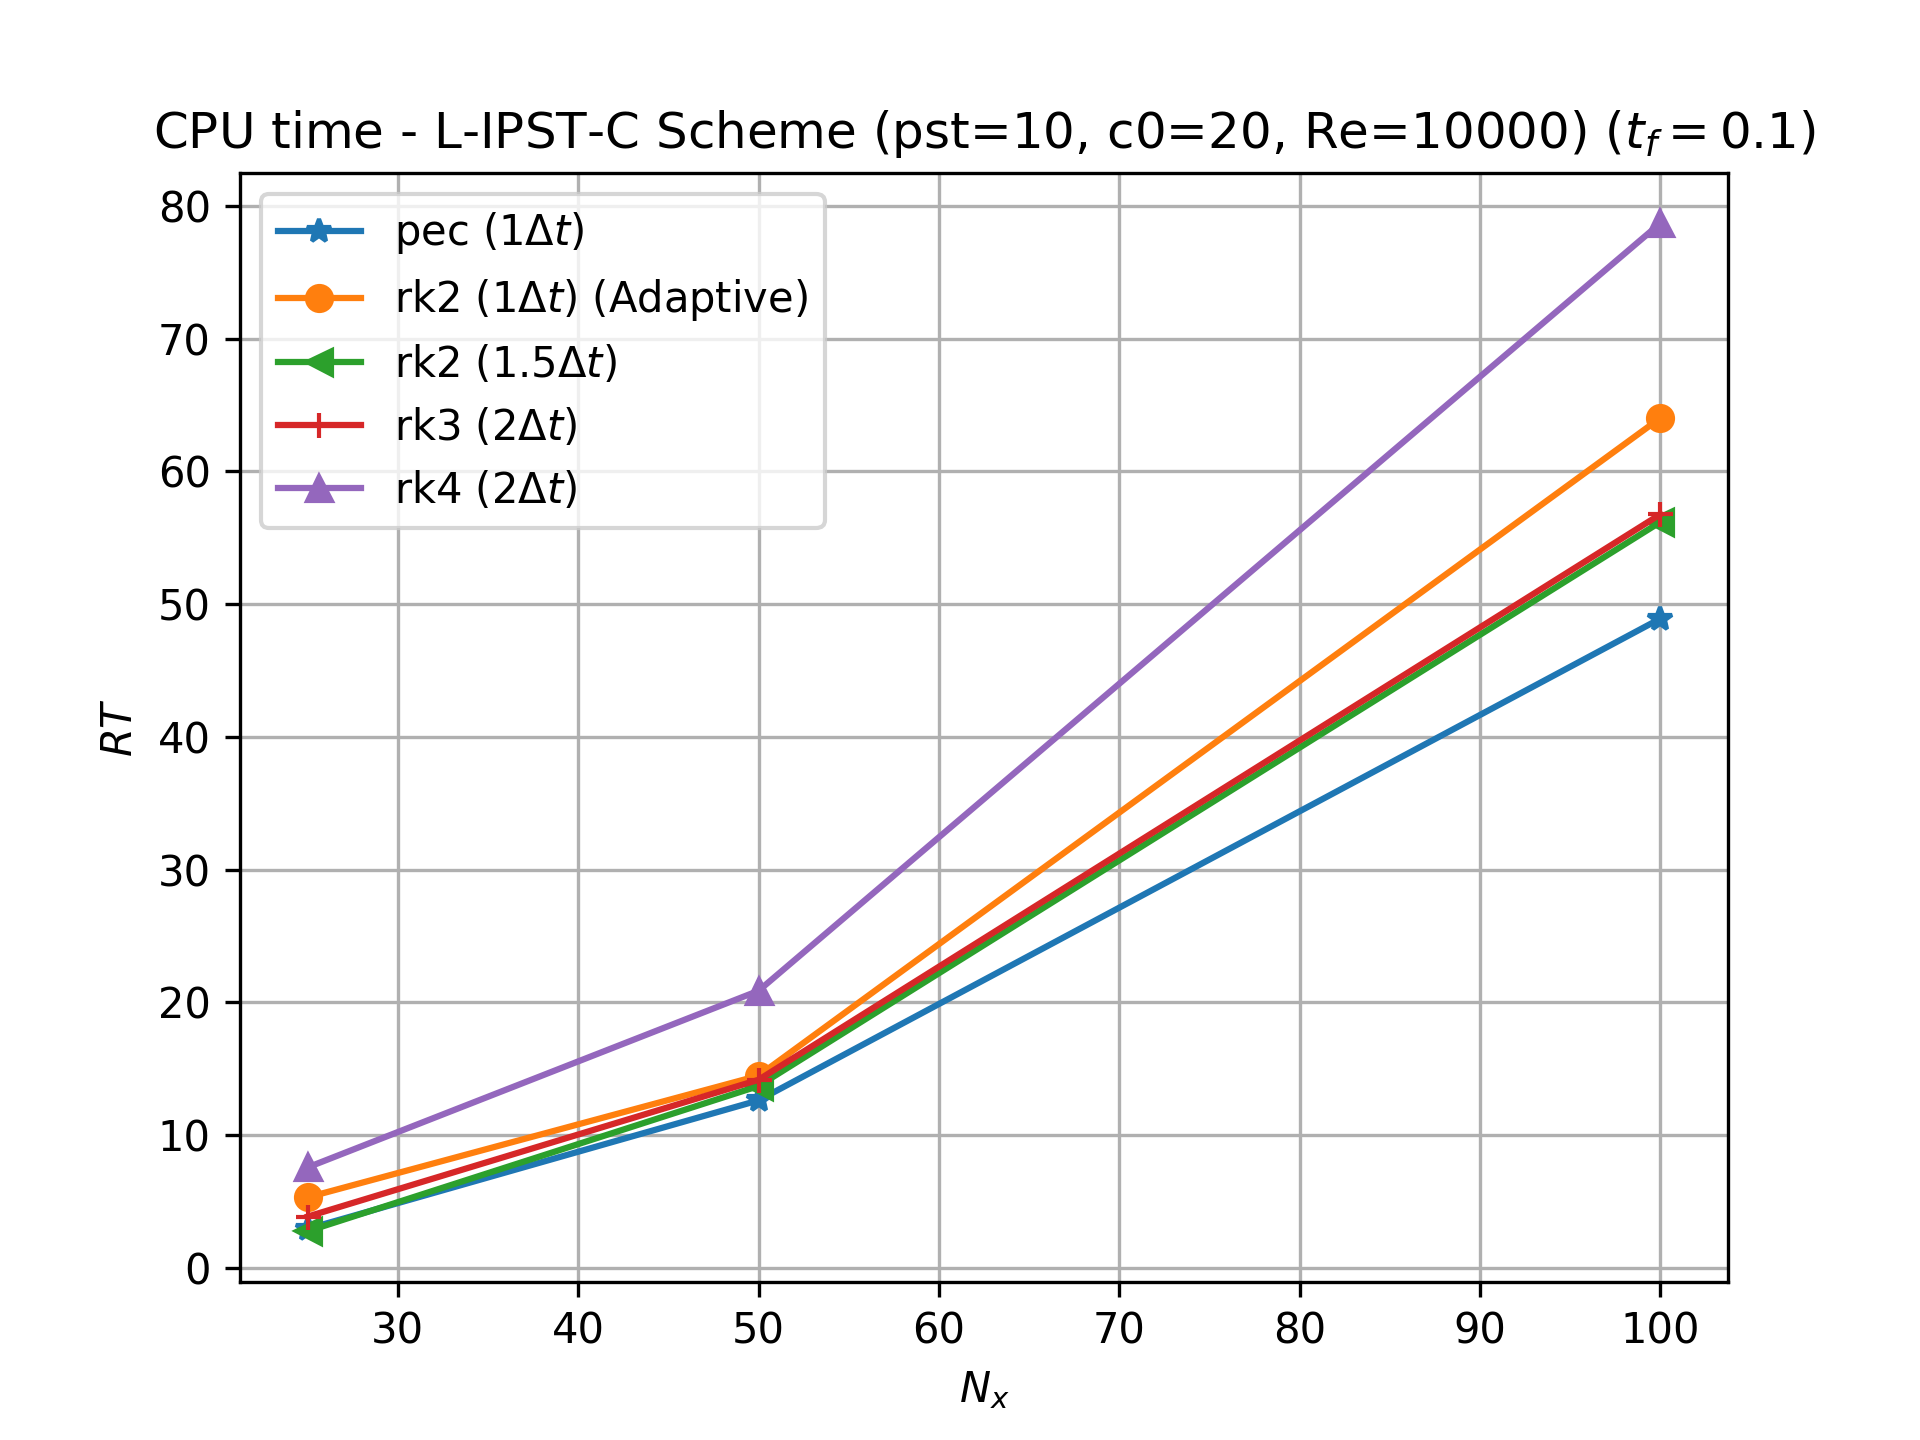
\includegraphics[width=6cm]{Code-Figures/lipstc/integrator/pois_rt_pst_10_c0_20_re_10000.png}
    \caption{$Re = 10000$}
  \end{subfigure}
  \caption{Run-time (in $s$) of the L-IPST-C scheme for various time-integrators.}
  \label{fig:lipstc-integrator-rt}
\end{figure}


\subsection{SPH-LES Scheme}
The SPH-LES scheme was considered over the other LES-based schemes since the scheme utilised the compressible NS equations, which were treated with a spatial averaging operator to obtain the filtered governing equations. They also considered three different models for the turbulent eddy viscosity, which included the standard Smagorinsky model, $\sigma$-model and the standard model discretised in the Monaghan-Cleary-Gingold (MCG) form (detailed in \secref{sec:Modified-Smagorinsky-Model}). Therefore, the model appeared comprehensive in terms of its implementation and hence, was chosen, along with the \texttt{SMAG} model, which is the standard Smagorinsky model, since their study revealed that this model was the most accurate relatively in terms of its prediction of the energy spectrum while using the \texttt{PEC} integrator.

\begin{figure}[htbp!]
  \begin{subfigure}{7cm}
    \centering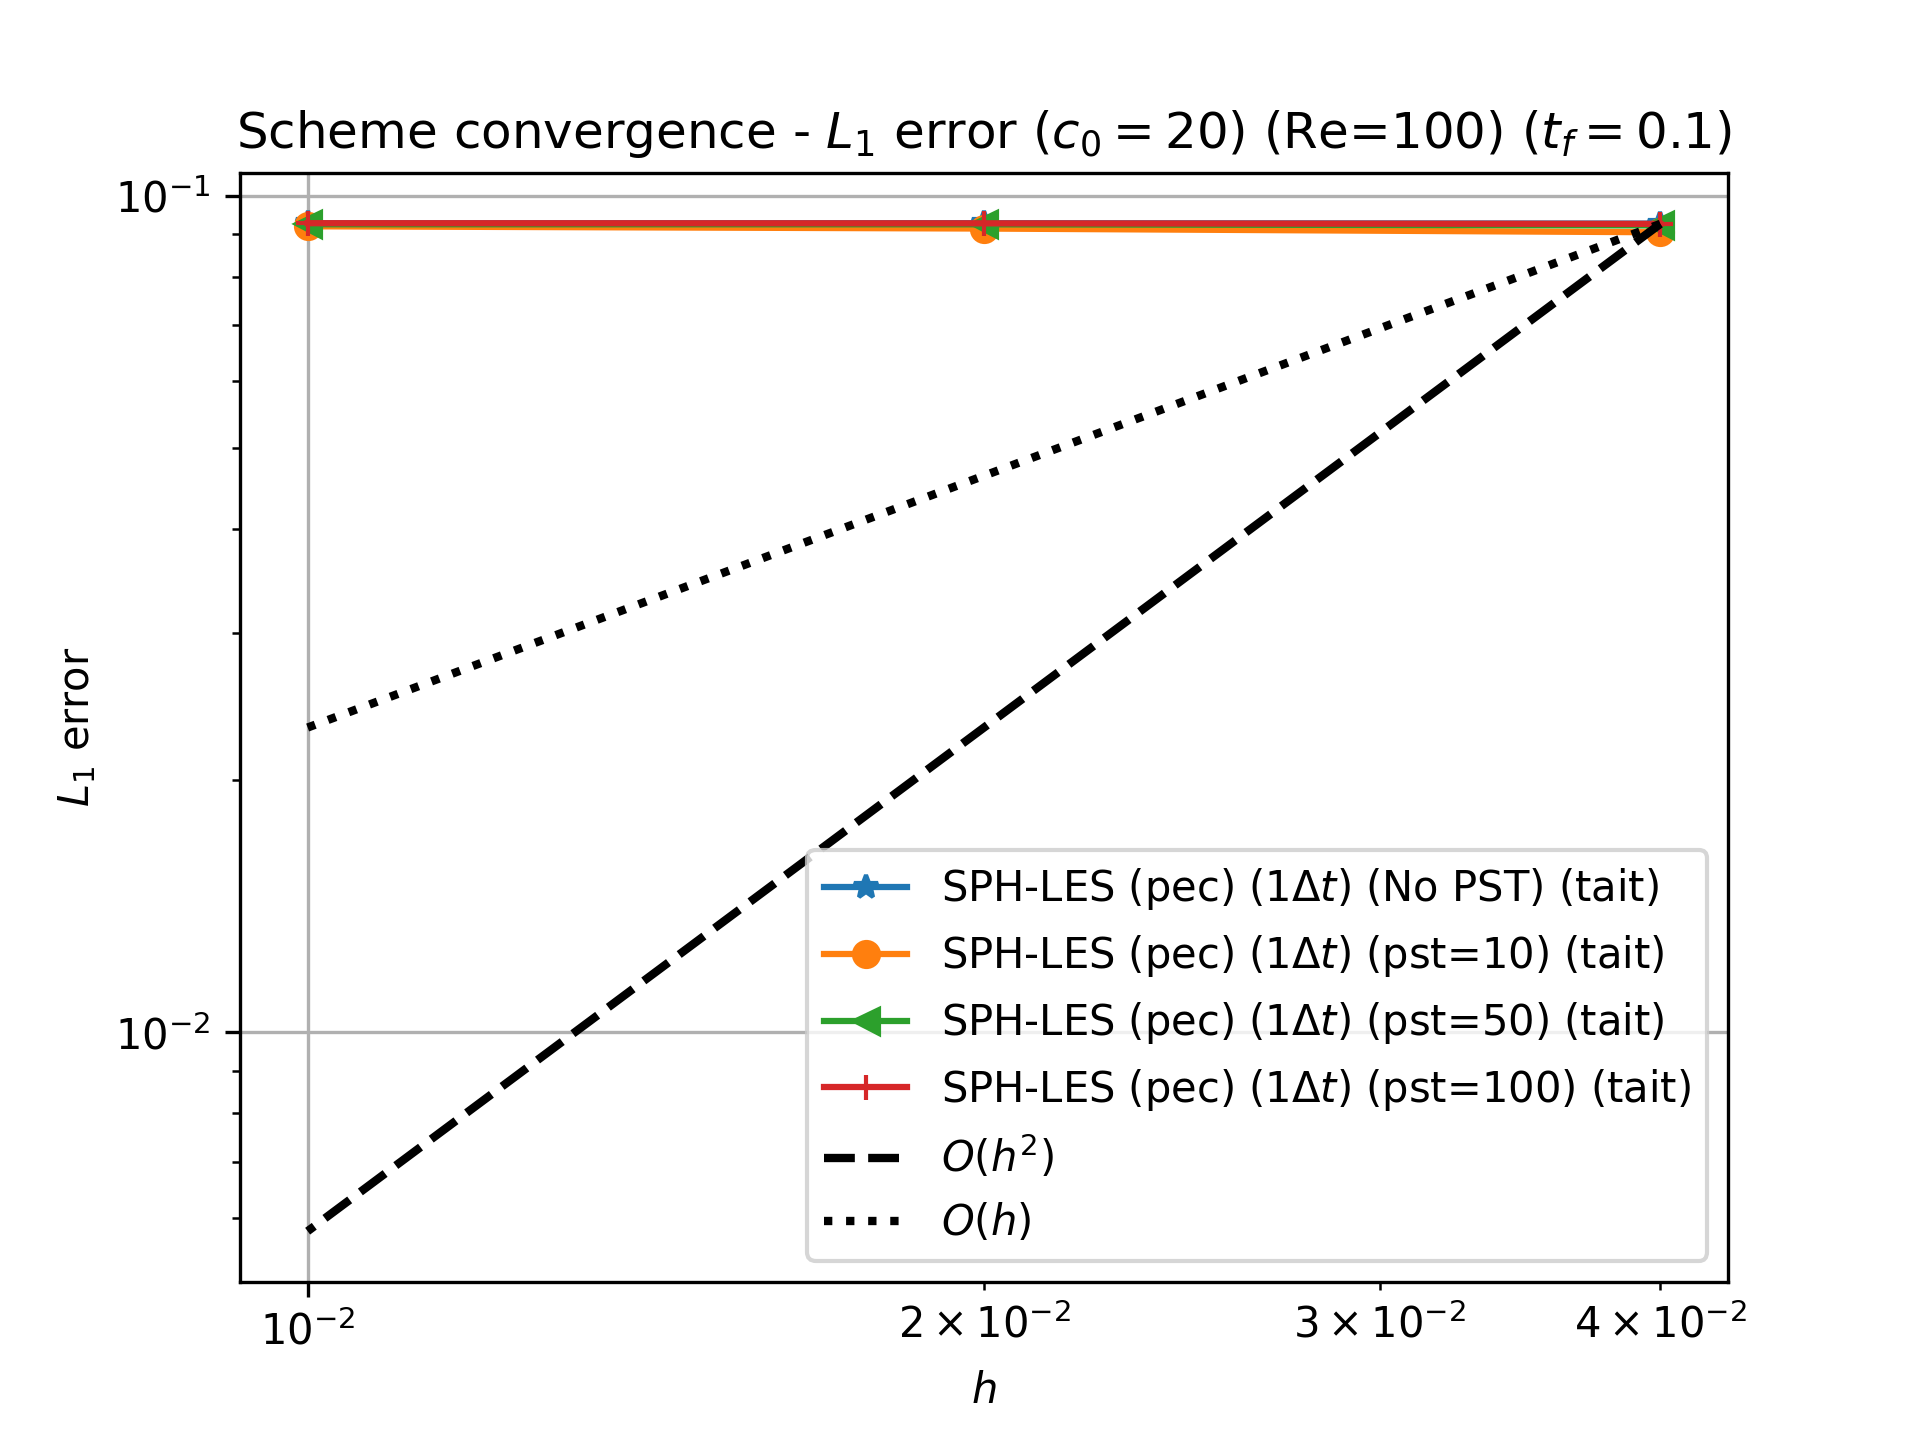
\includegraphics[width=6cm]{Code-Figures/okra2022/pst/dt_pois_conv_c0_20_re_100.png}
    \caption{$Re = 100$}
  \end{subfigure}
  \begin{subfigure}{7cm}
    \centering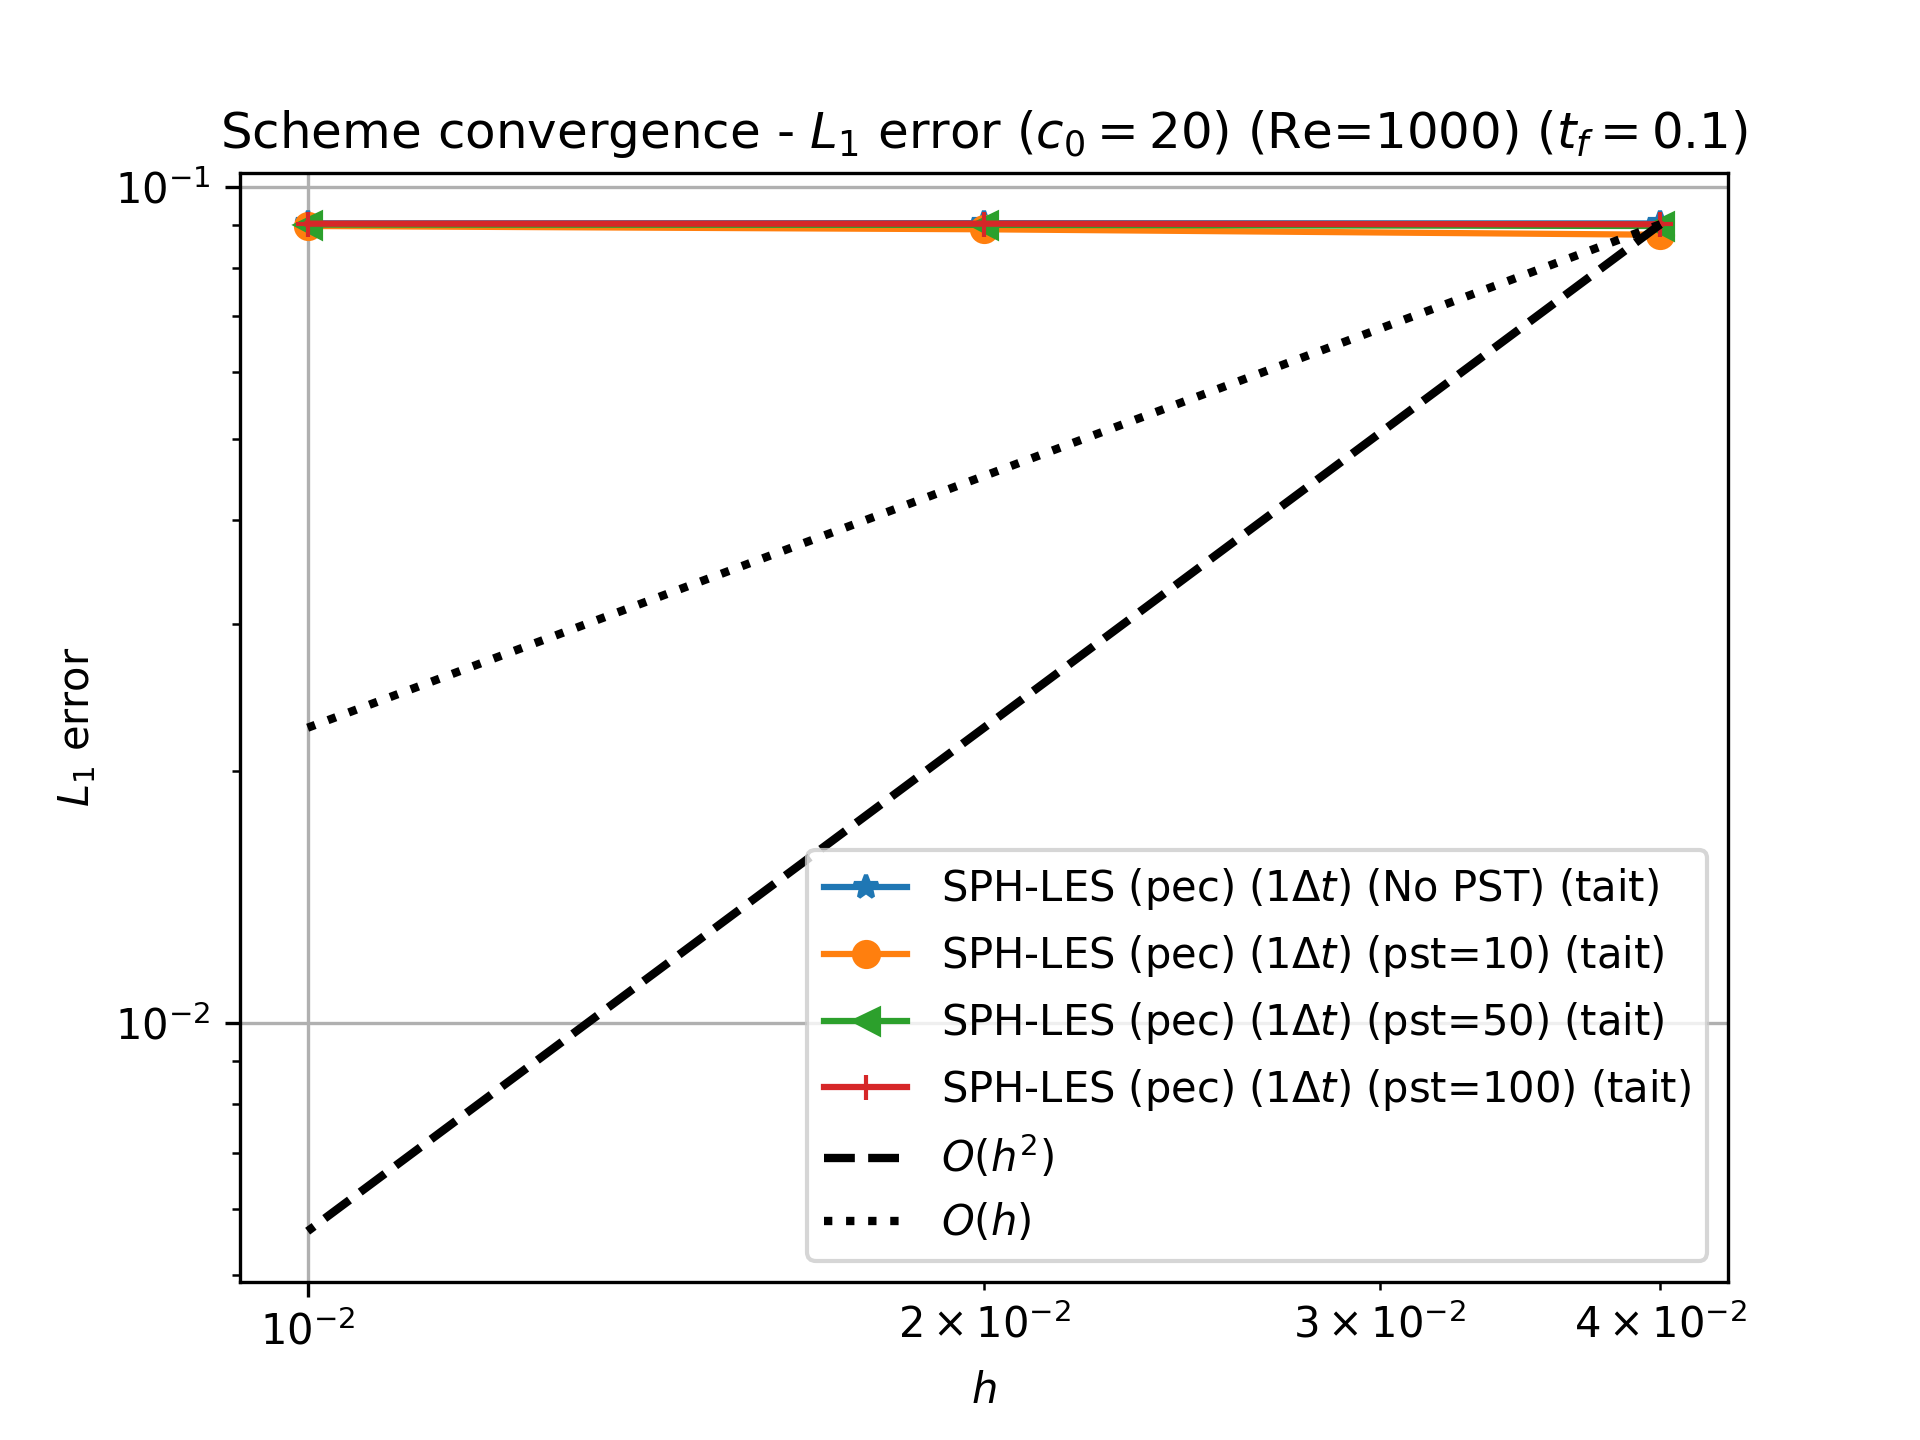
\includegraphics[width=6cm]{Code-Figures/okra2022/pst/dt_pois_conv_c0_20_re_1000.png}
    \caption{$Re = 1000$}
  \end{subfigure}
  \begin{subfigure}{7cm}
    \centering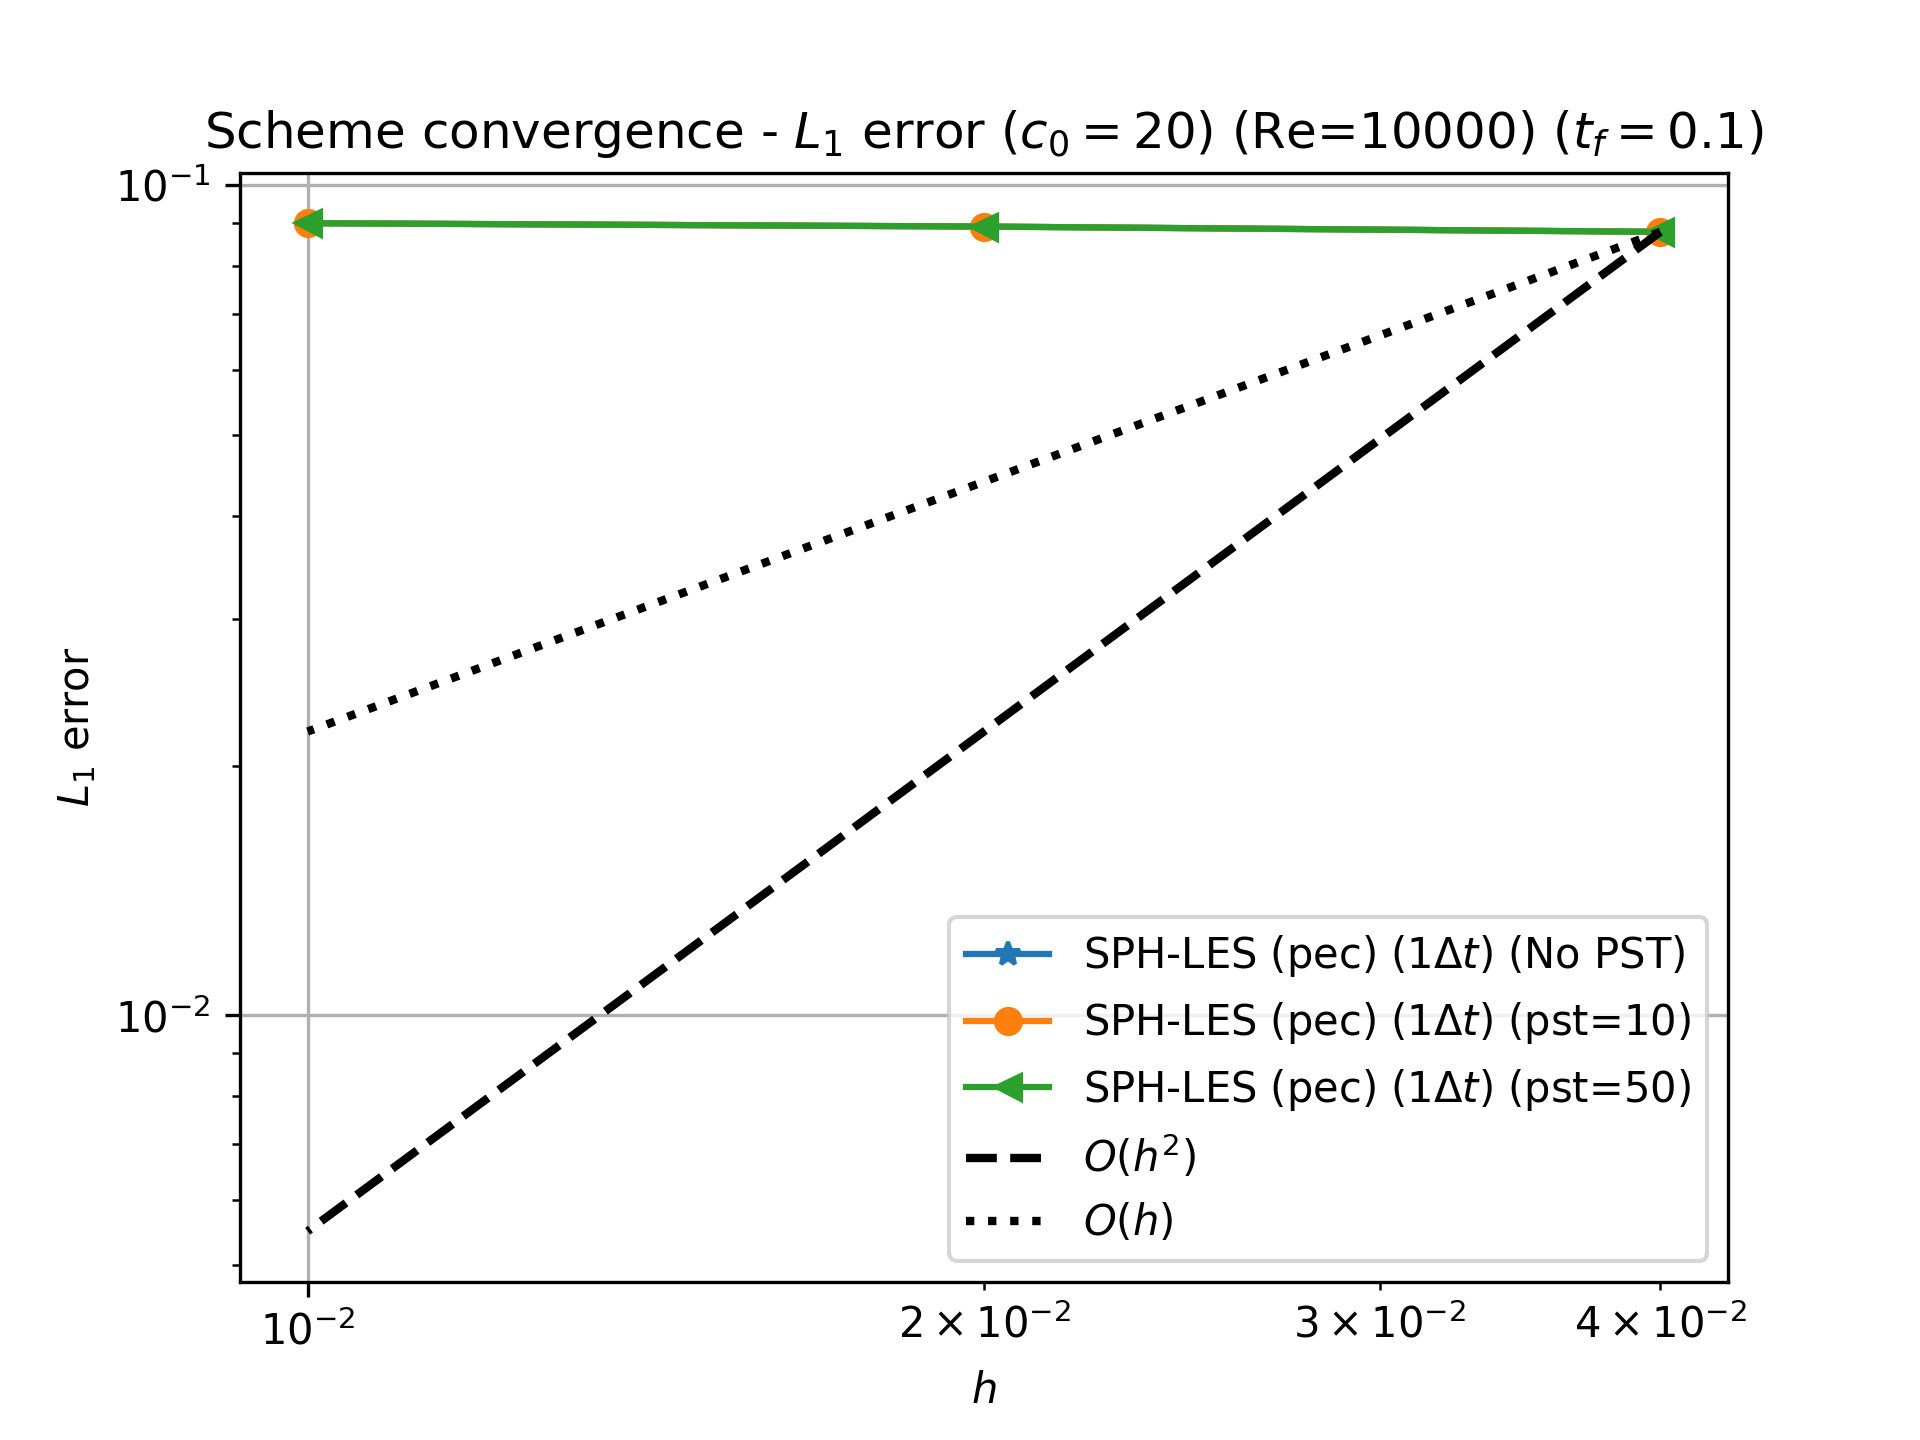
\includegraphics[width=6cm]{Code-Figures/okra2022/pst/dt_pois_conv_c0_20_re_10000.png}
    \caption{$Re = 10000$}
  \end{subfigure}
  \caption{Convergence of the SPH-LES scheme for various $f_{pst}$ values.}
  \label{fig:okra2022-pst}
\end{figure}


In order to identify the effects of the PST on the scheme, the following values were considered: $f_{pst} = [None, 10, 50, 100]$, with the speed of sound for the particles through PST to be $c_s = 20$. The results are shown in \figref{fig:okra2022-pst}, where it can be seen that the scheme worryingly appears to be zero-order convergent. The velocity magnitude field and the energy spectrum are plotted to help provide a deeper insight into the issue.
In \figref{fig:okra2022-pst-vmag}, it can be observed that the particles get clustered without PST, and there are marked regions devoid of particles. It is also evident that high values of $f_{PST}$ are also not desirable since the particles are still clustered and hence the formation of regions devoid of particles.
Also, in \figref{fig:okra2022-pst-espec}, it can be observed that the slope of the energy spectrum at the final time instance (yellow line) increases with increasing values of $f_{pst}$, which is indicative of the fact that the energy is being concentrated at the higher resolution scales, which is expected for the high $Re$ case.
Therefore, $f_{pst} = 10$ is chosen as the default value for the PST.

\begin{figure}[htbp!]
  \begin{subfigure}{7cm}
    \centering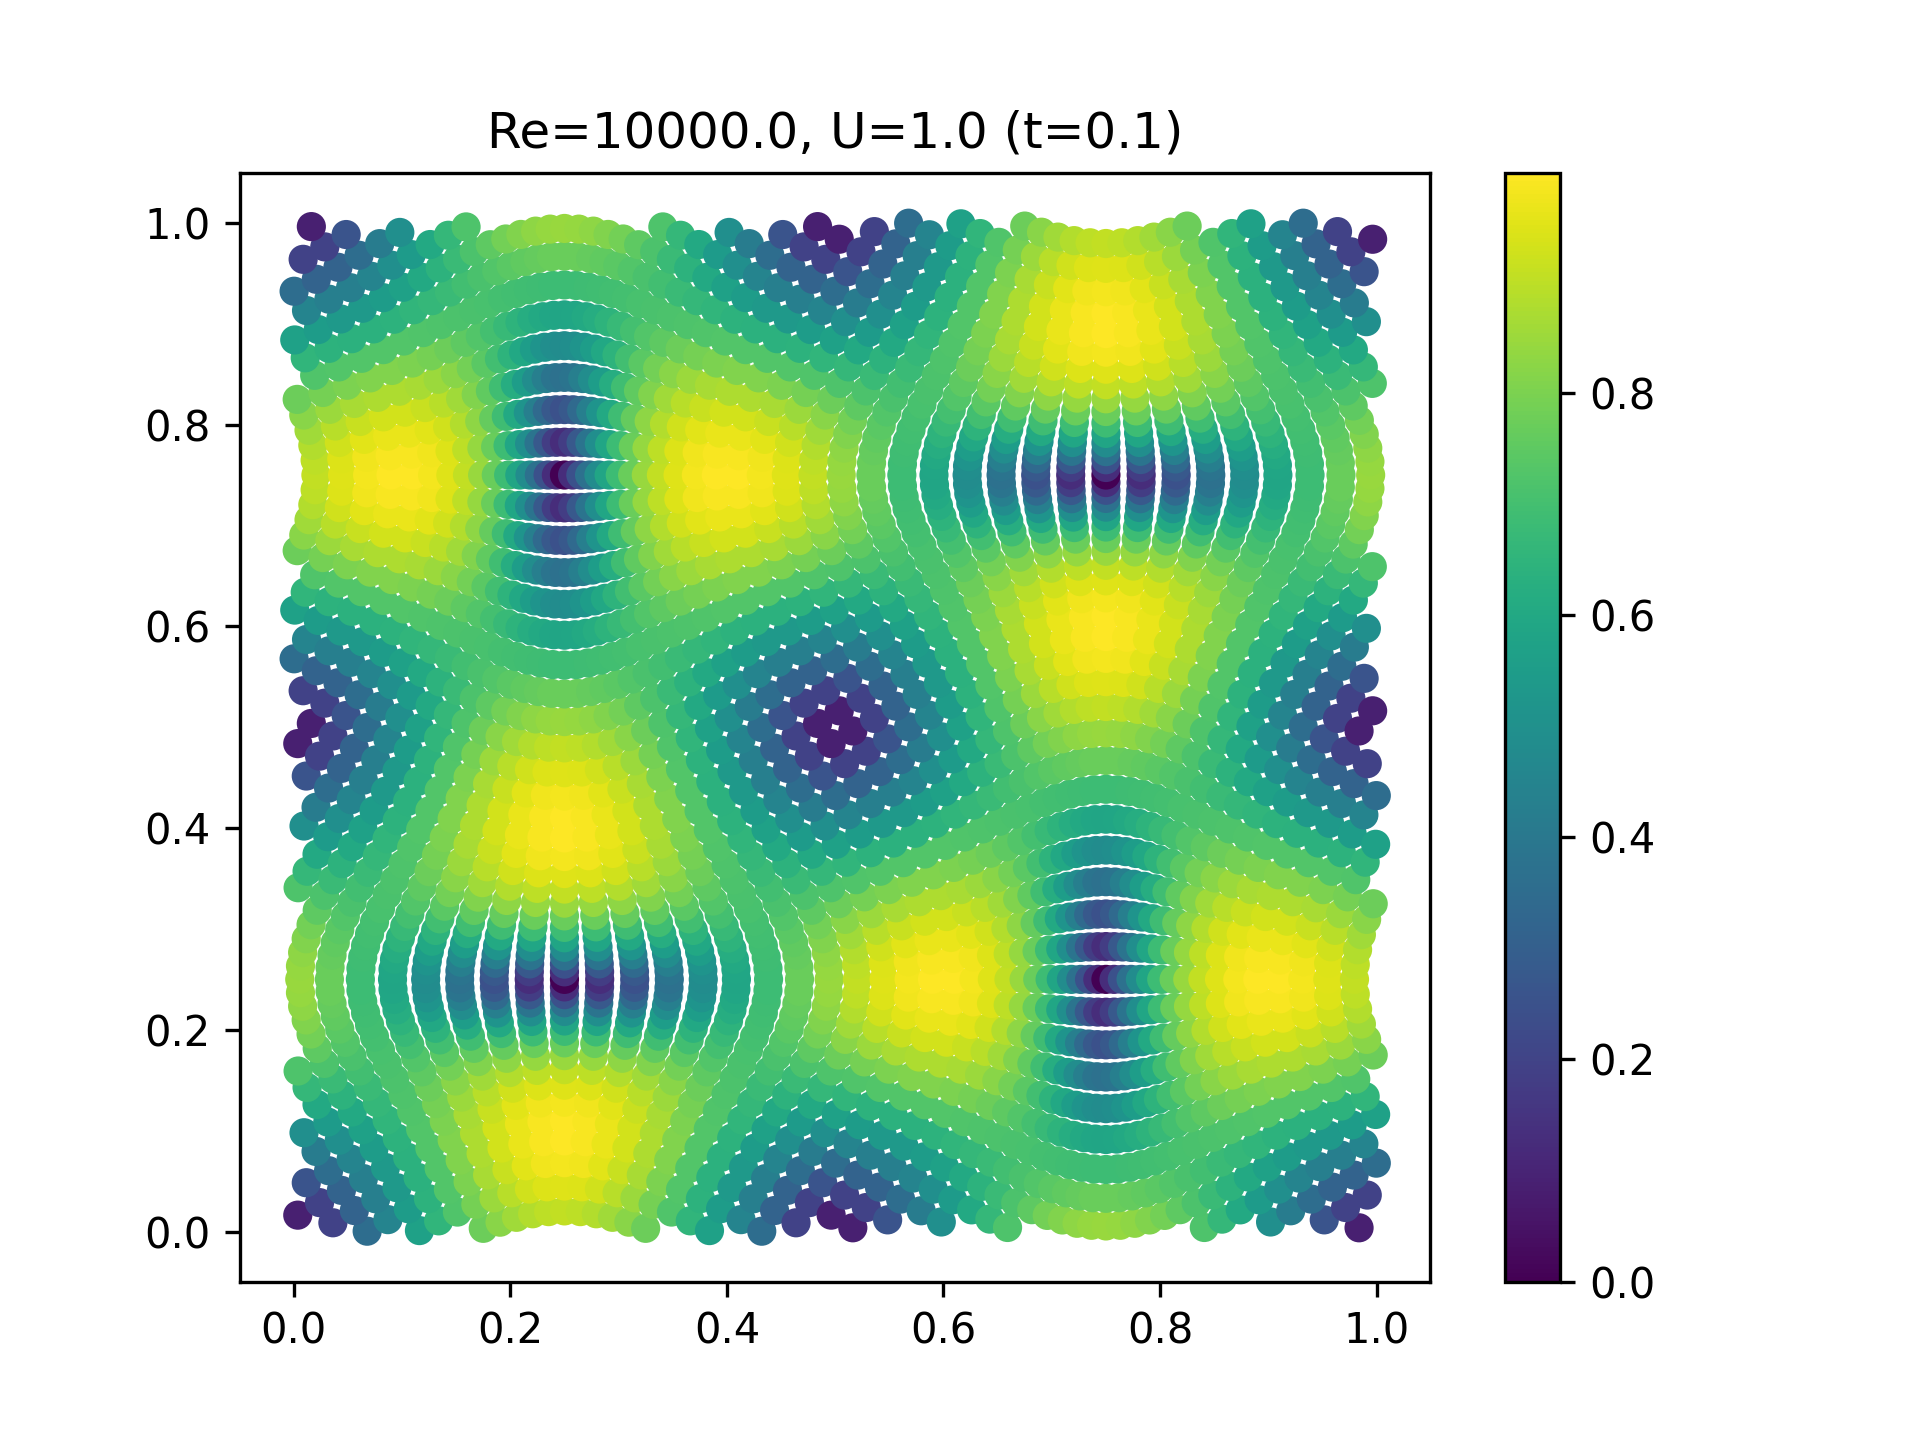
\includegraphics[width=6cm]{Code-Figures/okra2022/pst/c0_20_tait_pec_dtmul_1_nx_50_pst_-1_re_10000_ok2022/final_vmag.png}
    \caption{No PST}
  \end{subfigure}
  \begin{subfigure}{7cm}
    \centering\includegraphics[width=6cm]{Code-Figures/okra2022/pst/c0_20_tait_pec_dtmul_1_nx_50_pst_10_re_10000_ok2022/final_vmag.png}
    \caption{$f_{pst} = 10$}
  \end{subfigure}
  \begin{subfigure}{7cm}
    \centering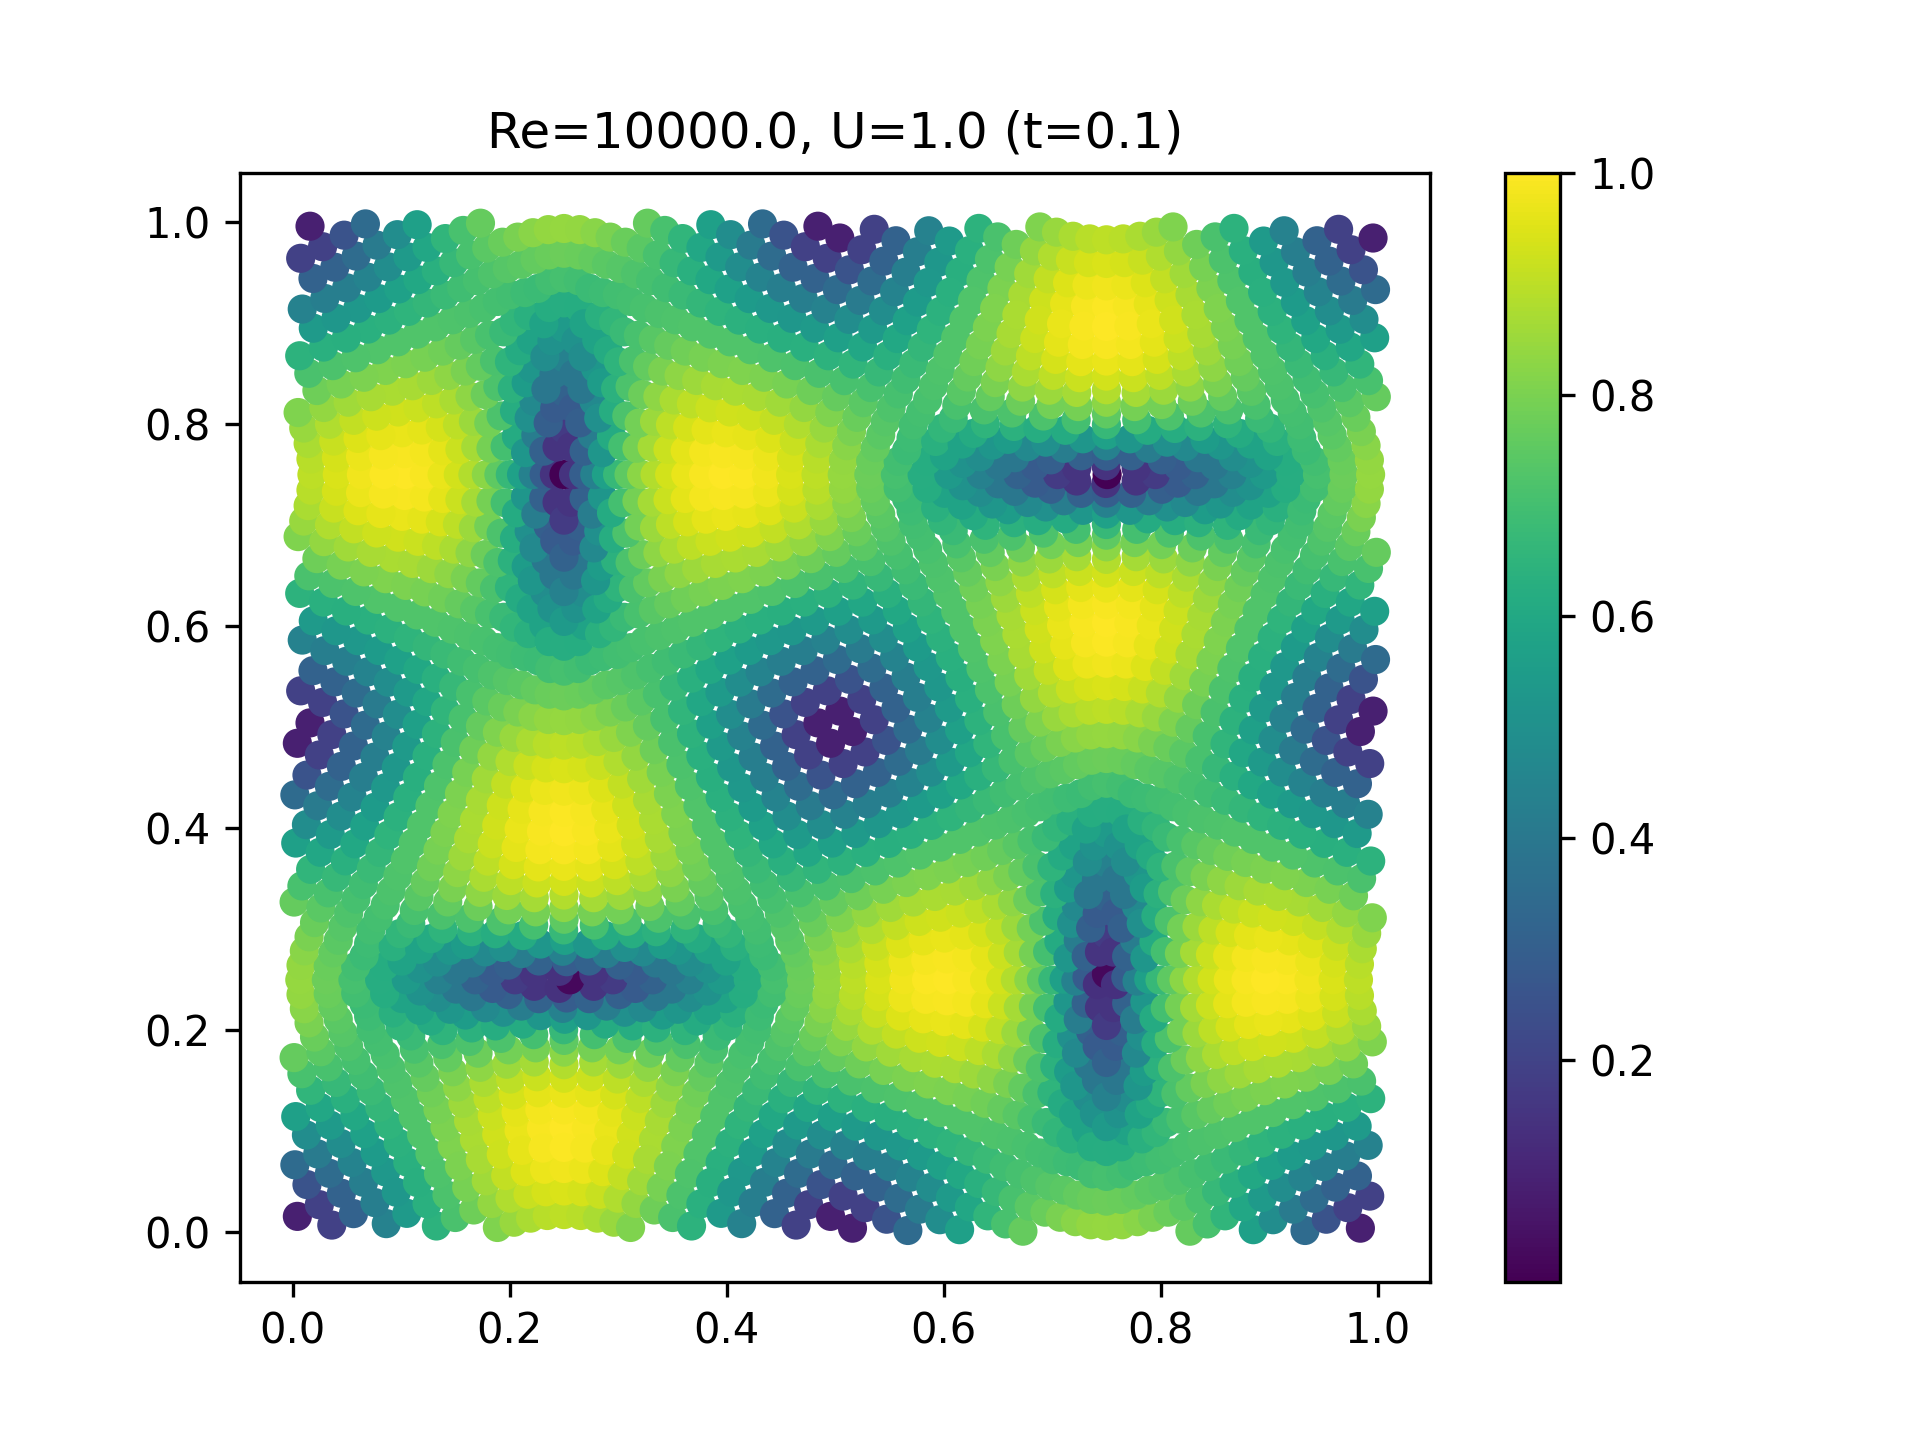
\includegraphics[width=6cm]{Code-Figures/okra2022/pst/c0_20_tait_pec_dtmul_1_nx_50_pst_50_re_10000_ok2022/final_vmag.png}
    \caption{$f_{pst} = 50$}
  \end{subfigure}
  \begin{subfigure}{7cm}
    \centering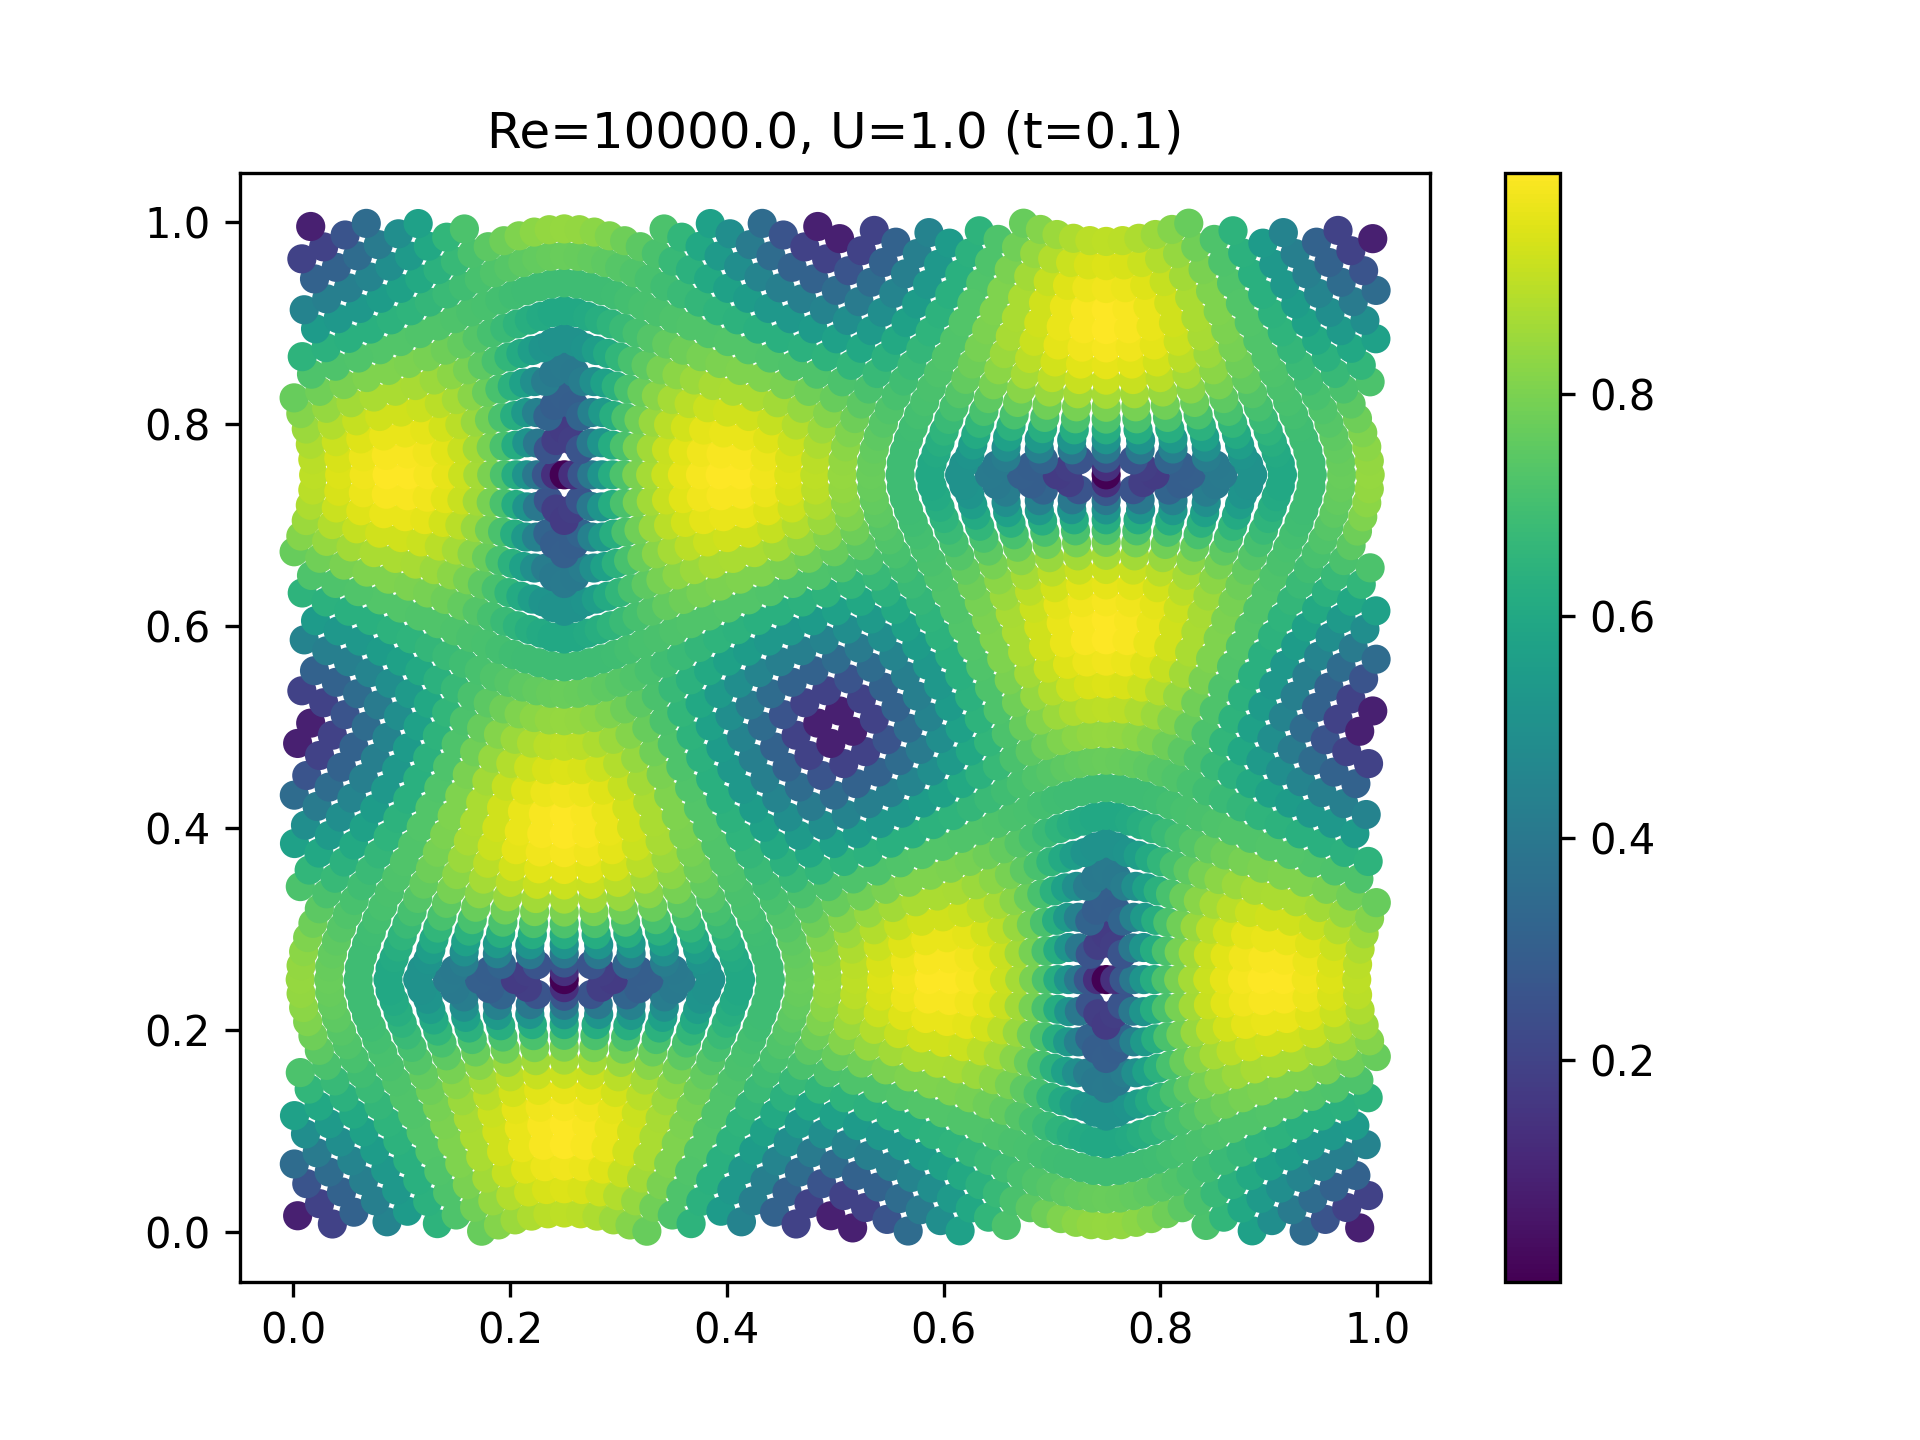
\includegraphics[width=6cm]{Code-Figures/okra2022/pst/c0_20_tait_pec_dtmul_1_nx_50_pst_100_re_10000_ok2022/final_vmag.png}
    \caption{$f_{pst} = 100$}
  \end{subfigure}
  \caption{Velocity magnitude field for the SPH-LES scheme for various $f_{pst}$ values $(N=50^2, t_f=0.1, Re=10000, c_s=20)$.}
  \label{fig:okra2022-pst-vmag}
\end{figure}

\begin{figure}[htbp!]
  \begin{subfigure}{7cm}
    \centering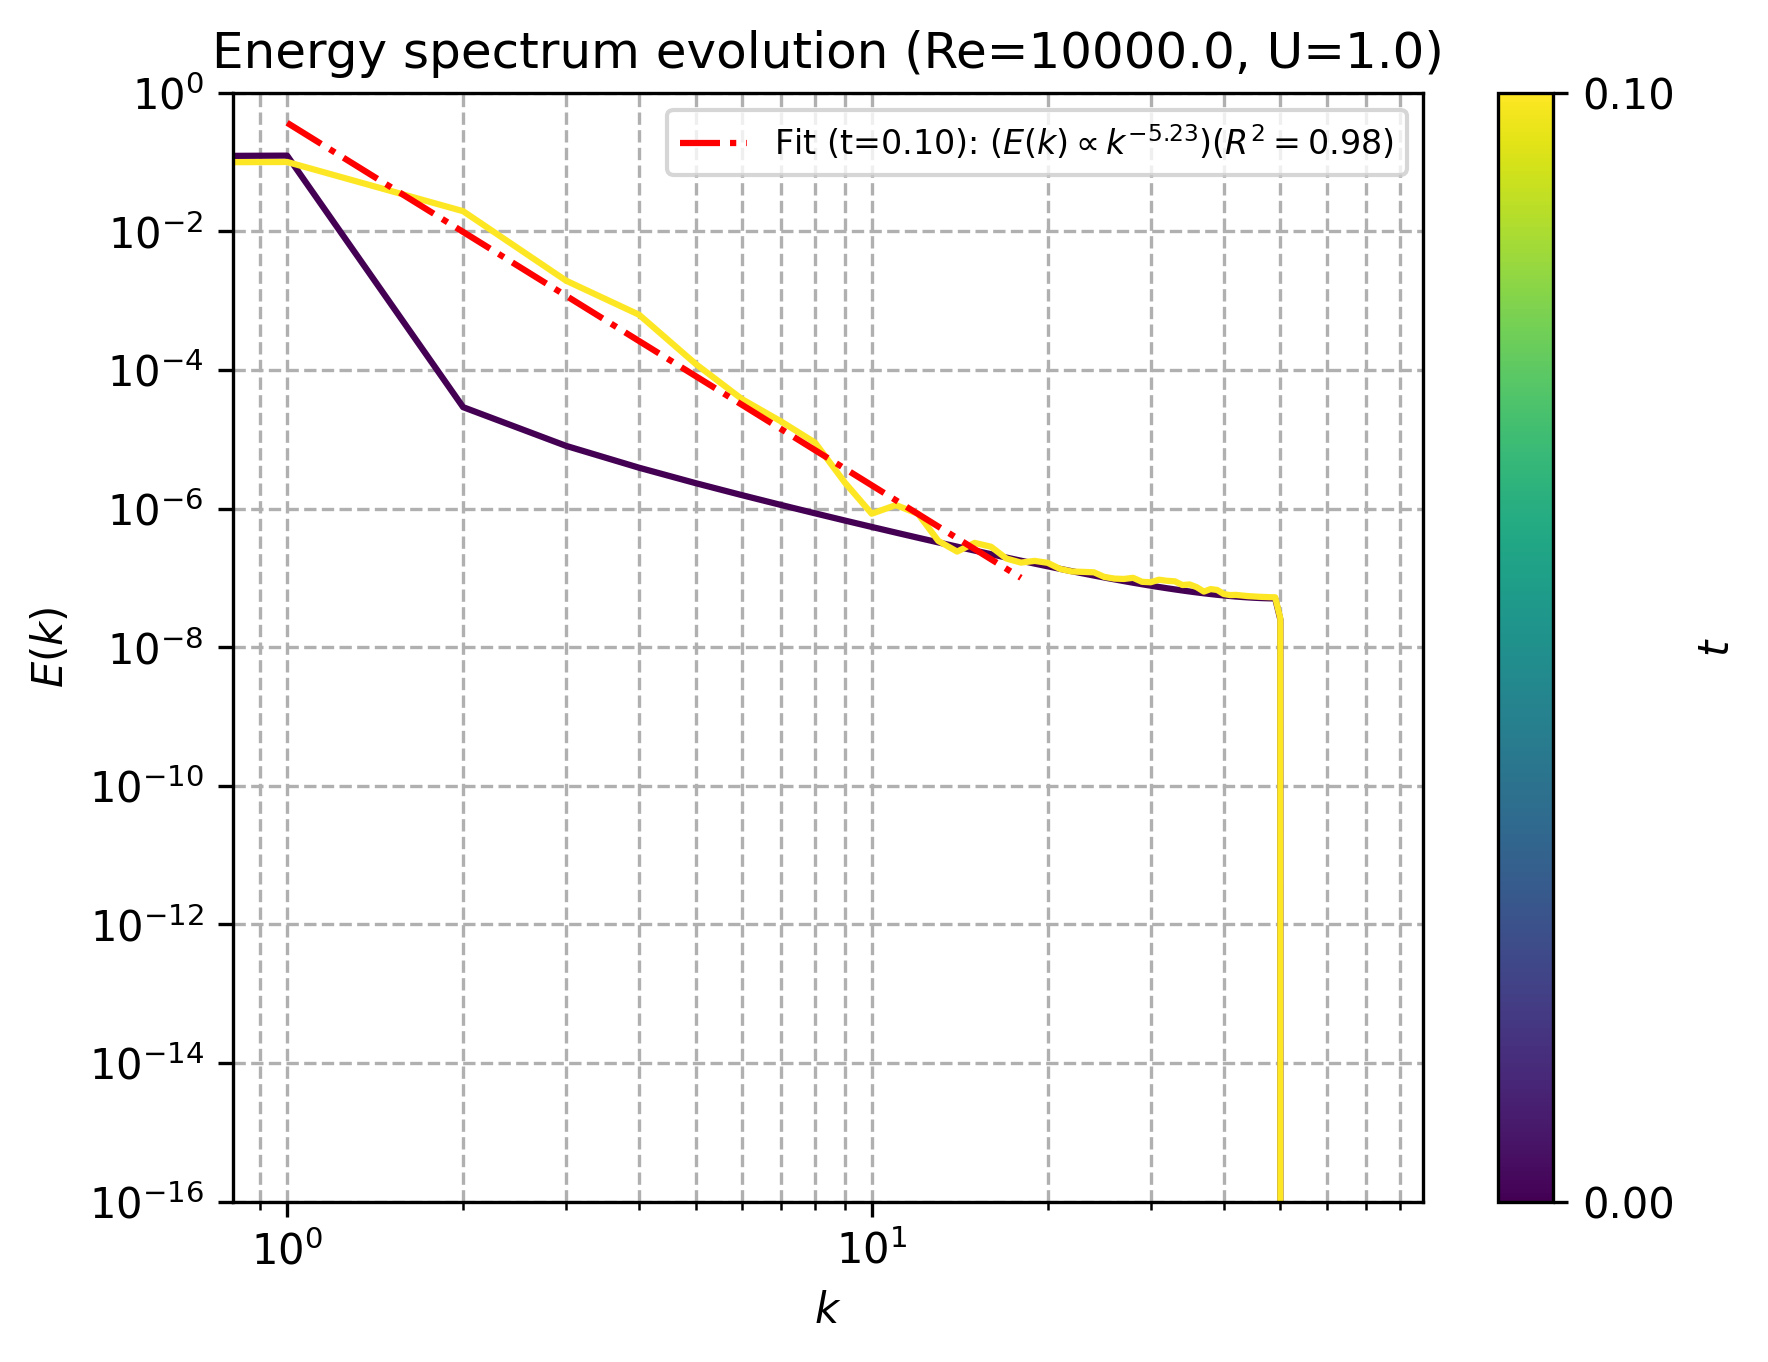
\includegraphics[width=6cm]{Code-Figures/okra2022/pst/c0_20_tait_pec_dtmul_1_nx_100_pst_-1_re_10000_ok2022/energy_spectrum_evolution.png}
    \caption{No PST}
  \end{subfigure}
  \begin{subfigure}{7cm}
    \centering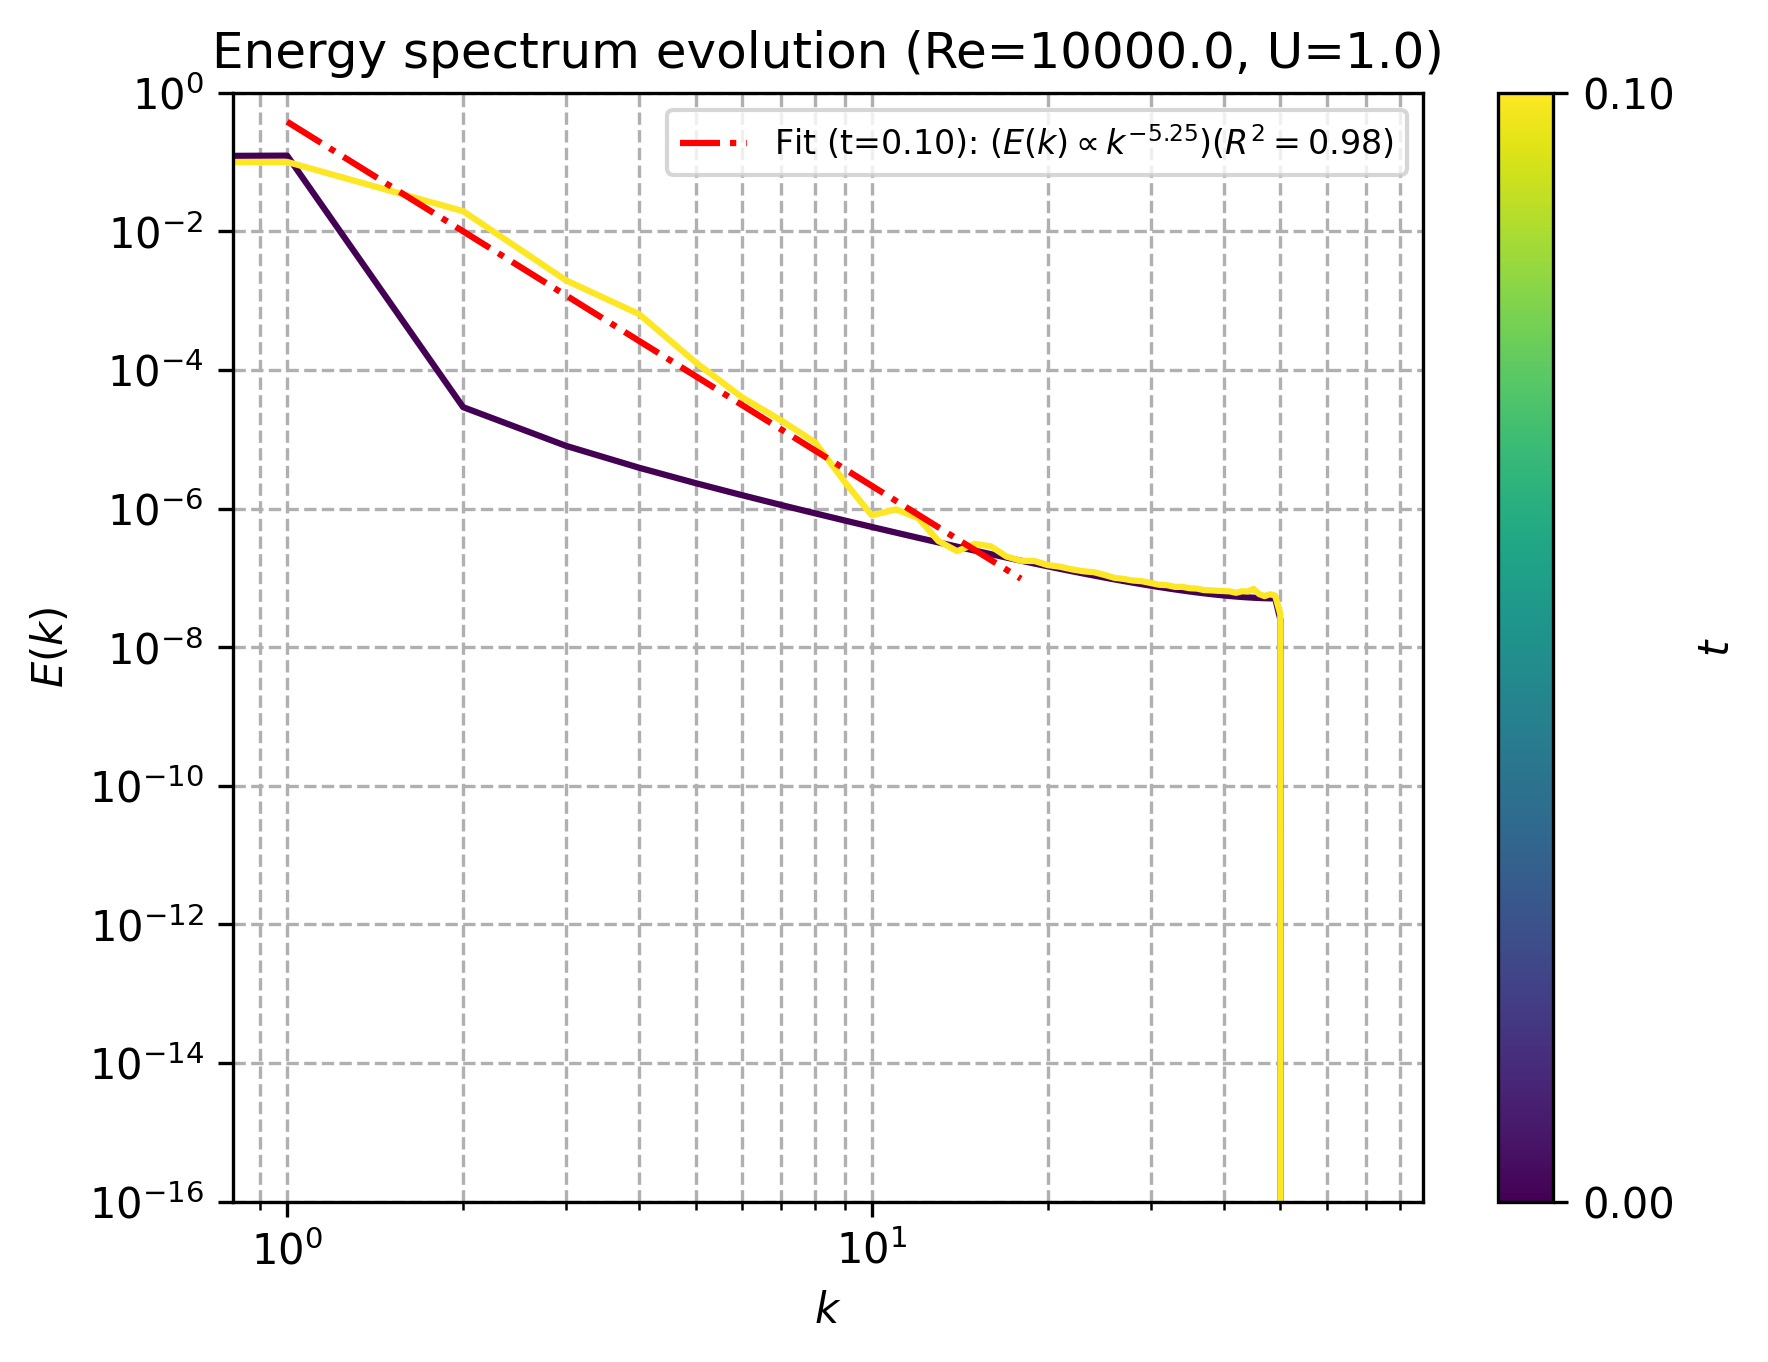
\includegraphics[width=6cm]{Code-Figures/okra2022/pst/c0_20_tait_pec_dtmul_1_nx_100_pst_10_re_10000_ok2022/energy_spectrum_evolution.png}
    \caption{$f_{pst} = 10$}
  \end{subfigure}
  \begin{subfigure}{7cm}
    \centering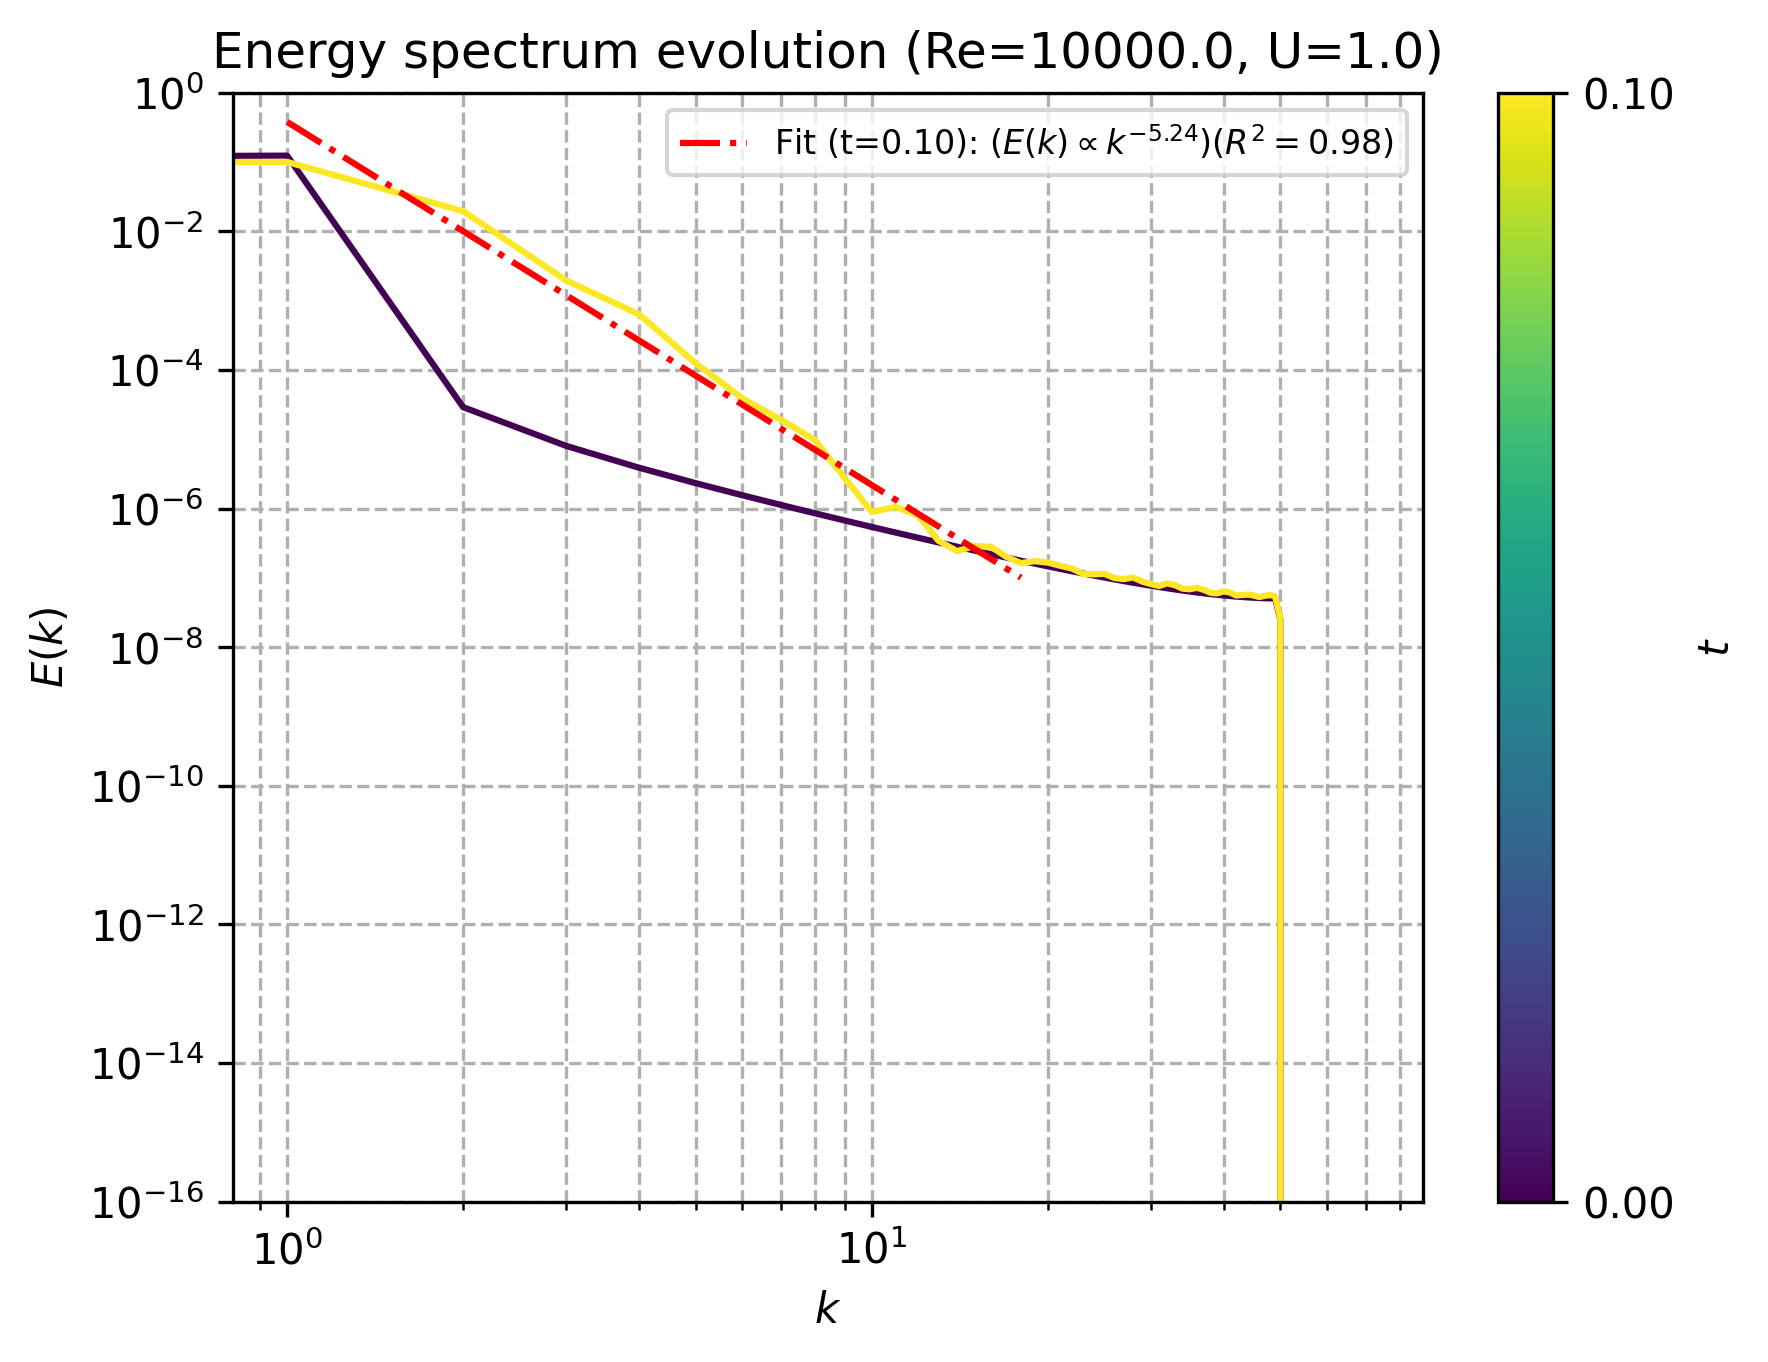
\includegraphics[width=6cm]{Code-Figures/okra2022/pst/c0_20_tait_pec_dtmul_1_nx_100_pst_50_re_10000_ok2022/energy_spectrum_evolution.png}
    \caption{$f_{pst} = 50$}
  \end{subfigure}
  \begin{subfigure}{7cm}
    \centering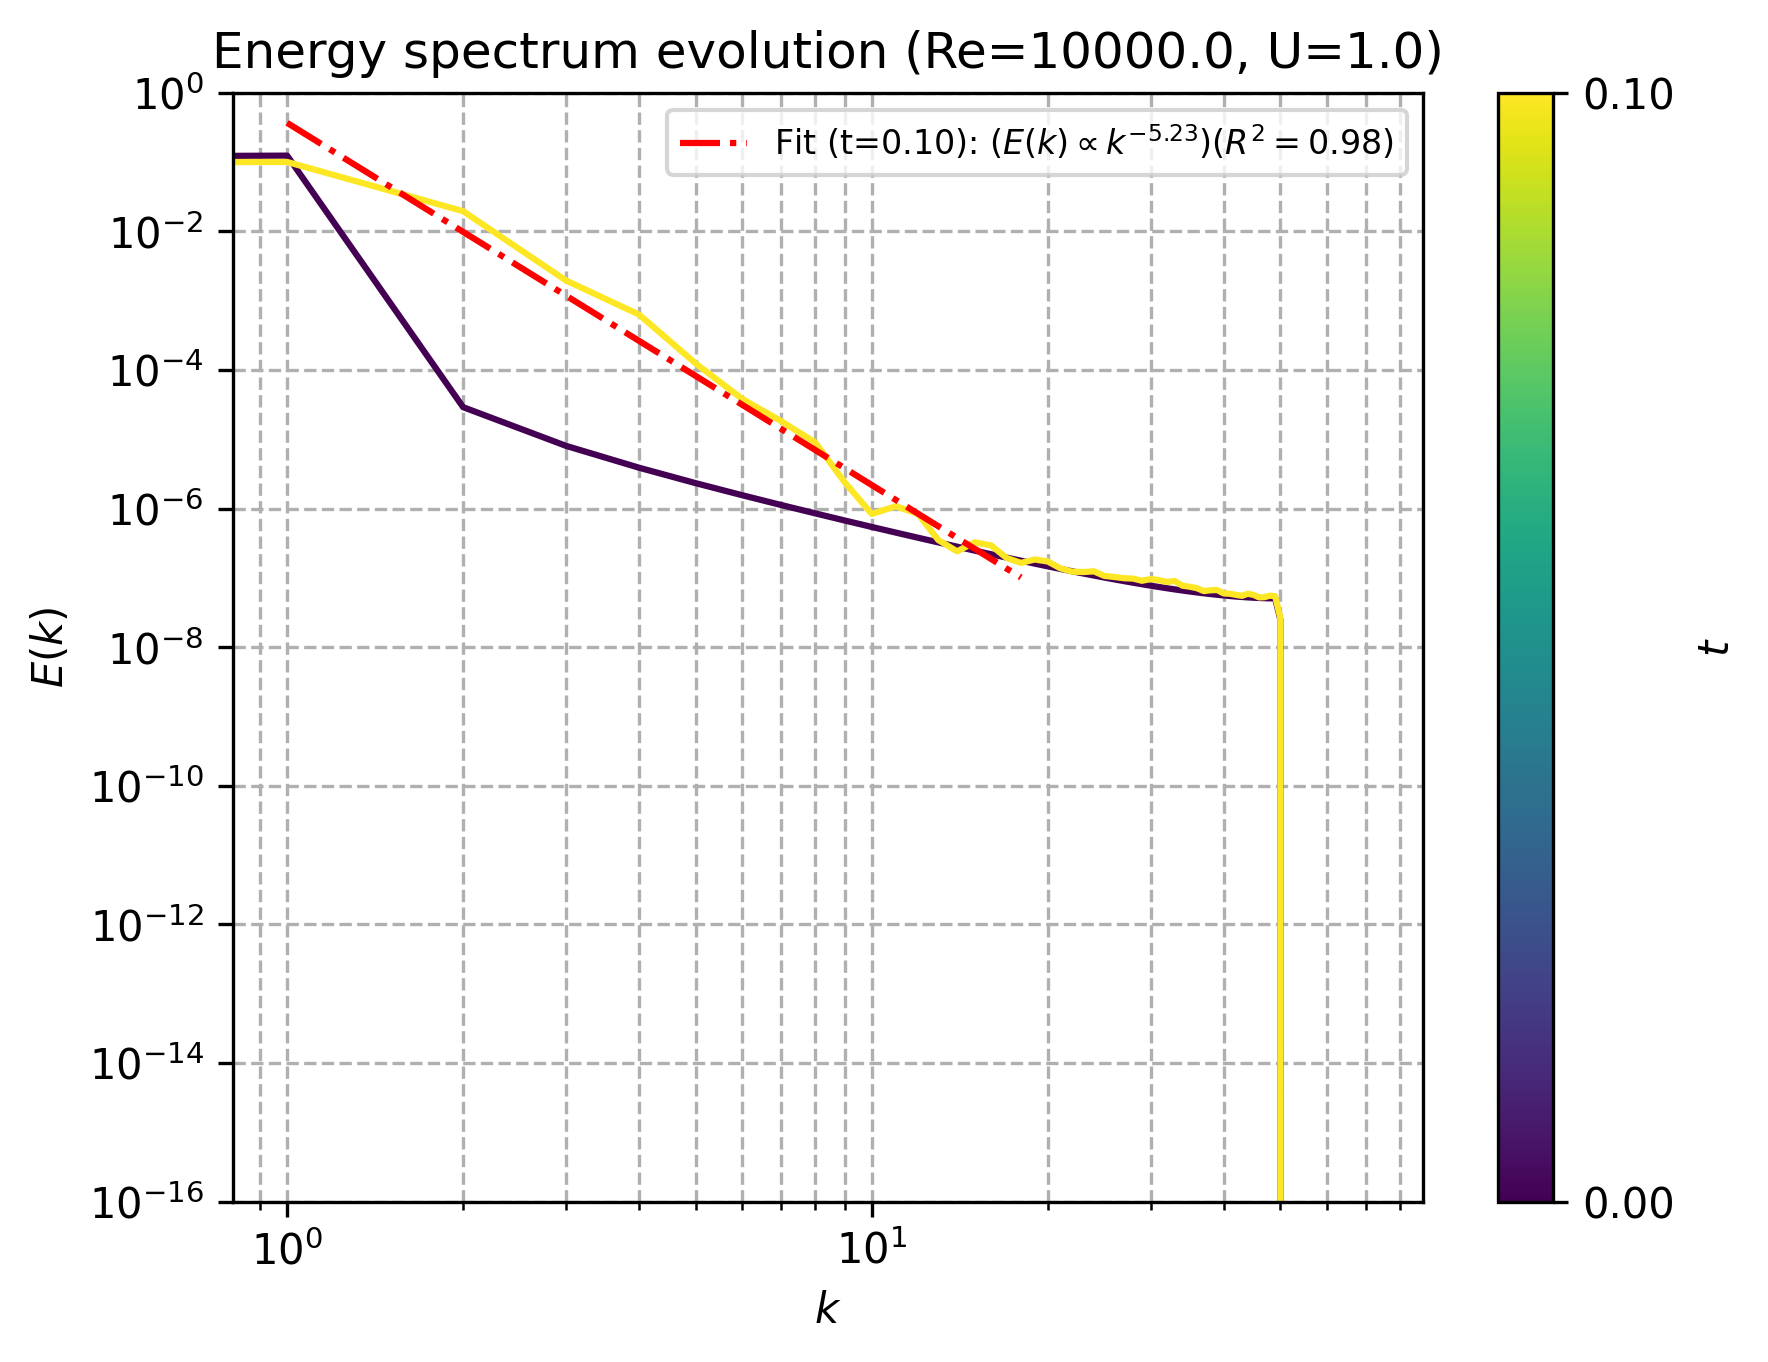
\includegraphics[width=6cm]{Code-Figures/okra2022/pst/c0_20_tait_pec_dtmul_1_nx_100_pst_100_re_10000_ok2022/energy_spectrum_evolution.png}
    \caption{$f_{pst} = 100$}
  \end{subfigure}
  \caption{Evolution of the energy spectrum for the SPH-LES scheme for various$f_{pst}$ values $(N=100^2, t_f=0.1, Re=10000, c_s=20)$. The initial energy spectrum is plotted in dark blue, and the final energy spectrum is plotted in yellow.}
  \label{fig:okra2022-pst-espec}
\end{figure}


\begin{figure}[htbp!]
  \begin{subfigure}{7cm}
    \centering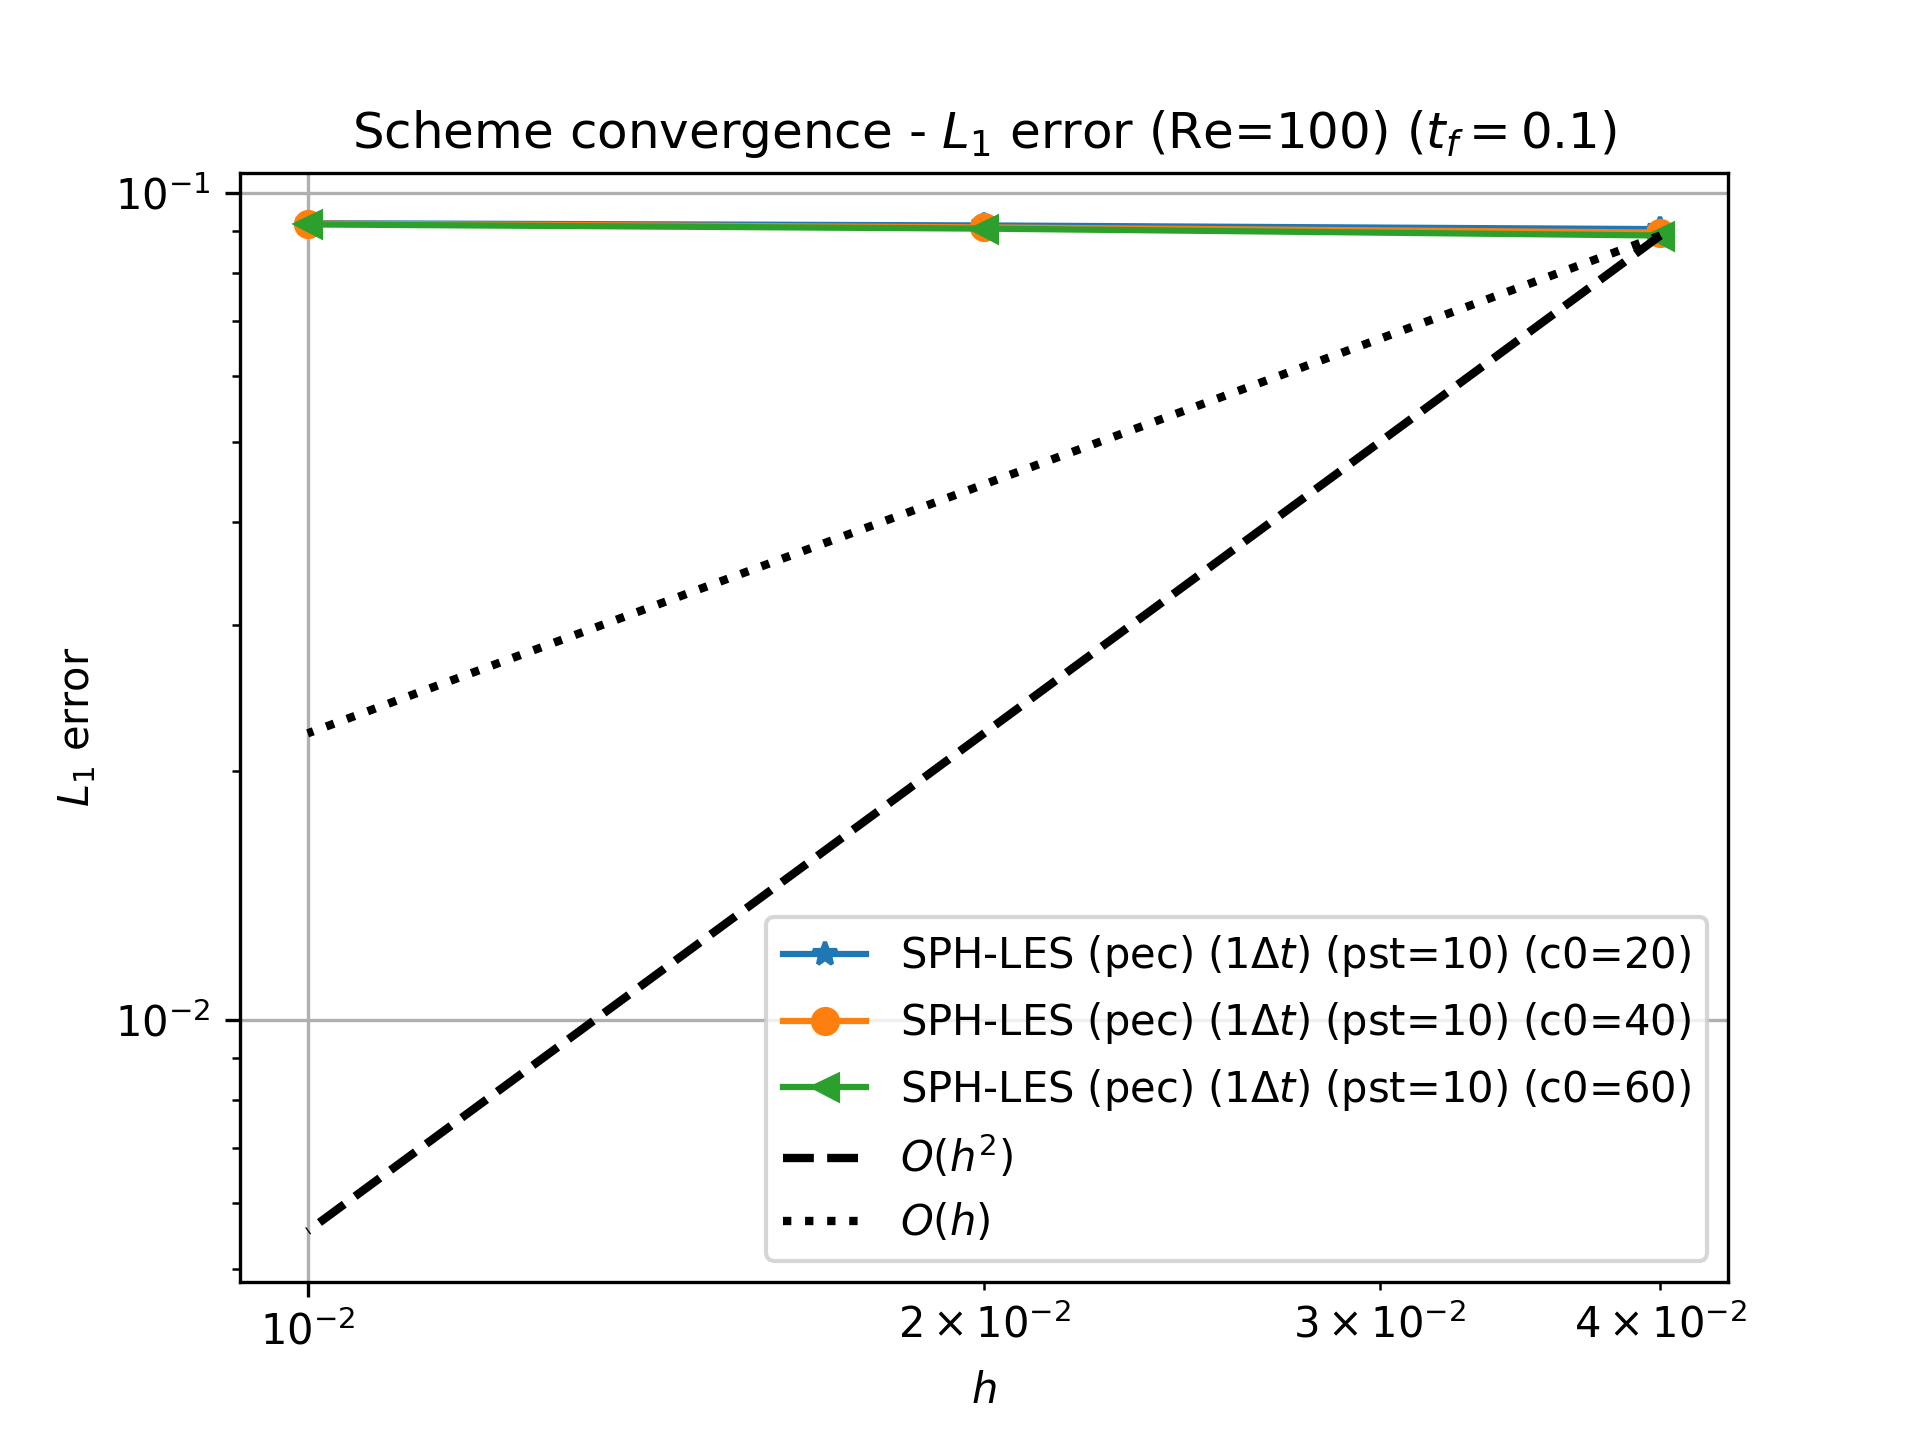
\includegraphics[width=6cm]{Code-Figures/okra2022/c0/dt_pois_conv_c0_pec_re_100.png}
    \caption{$Re = 100$}
  \end{subfigure}
  \begin{subfigure}{7cm}
    \centering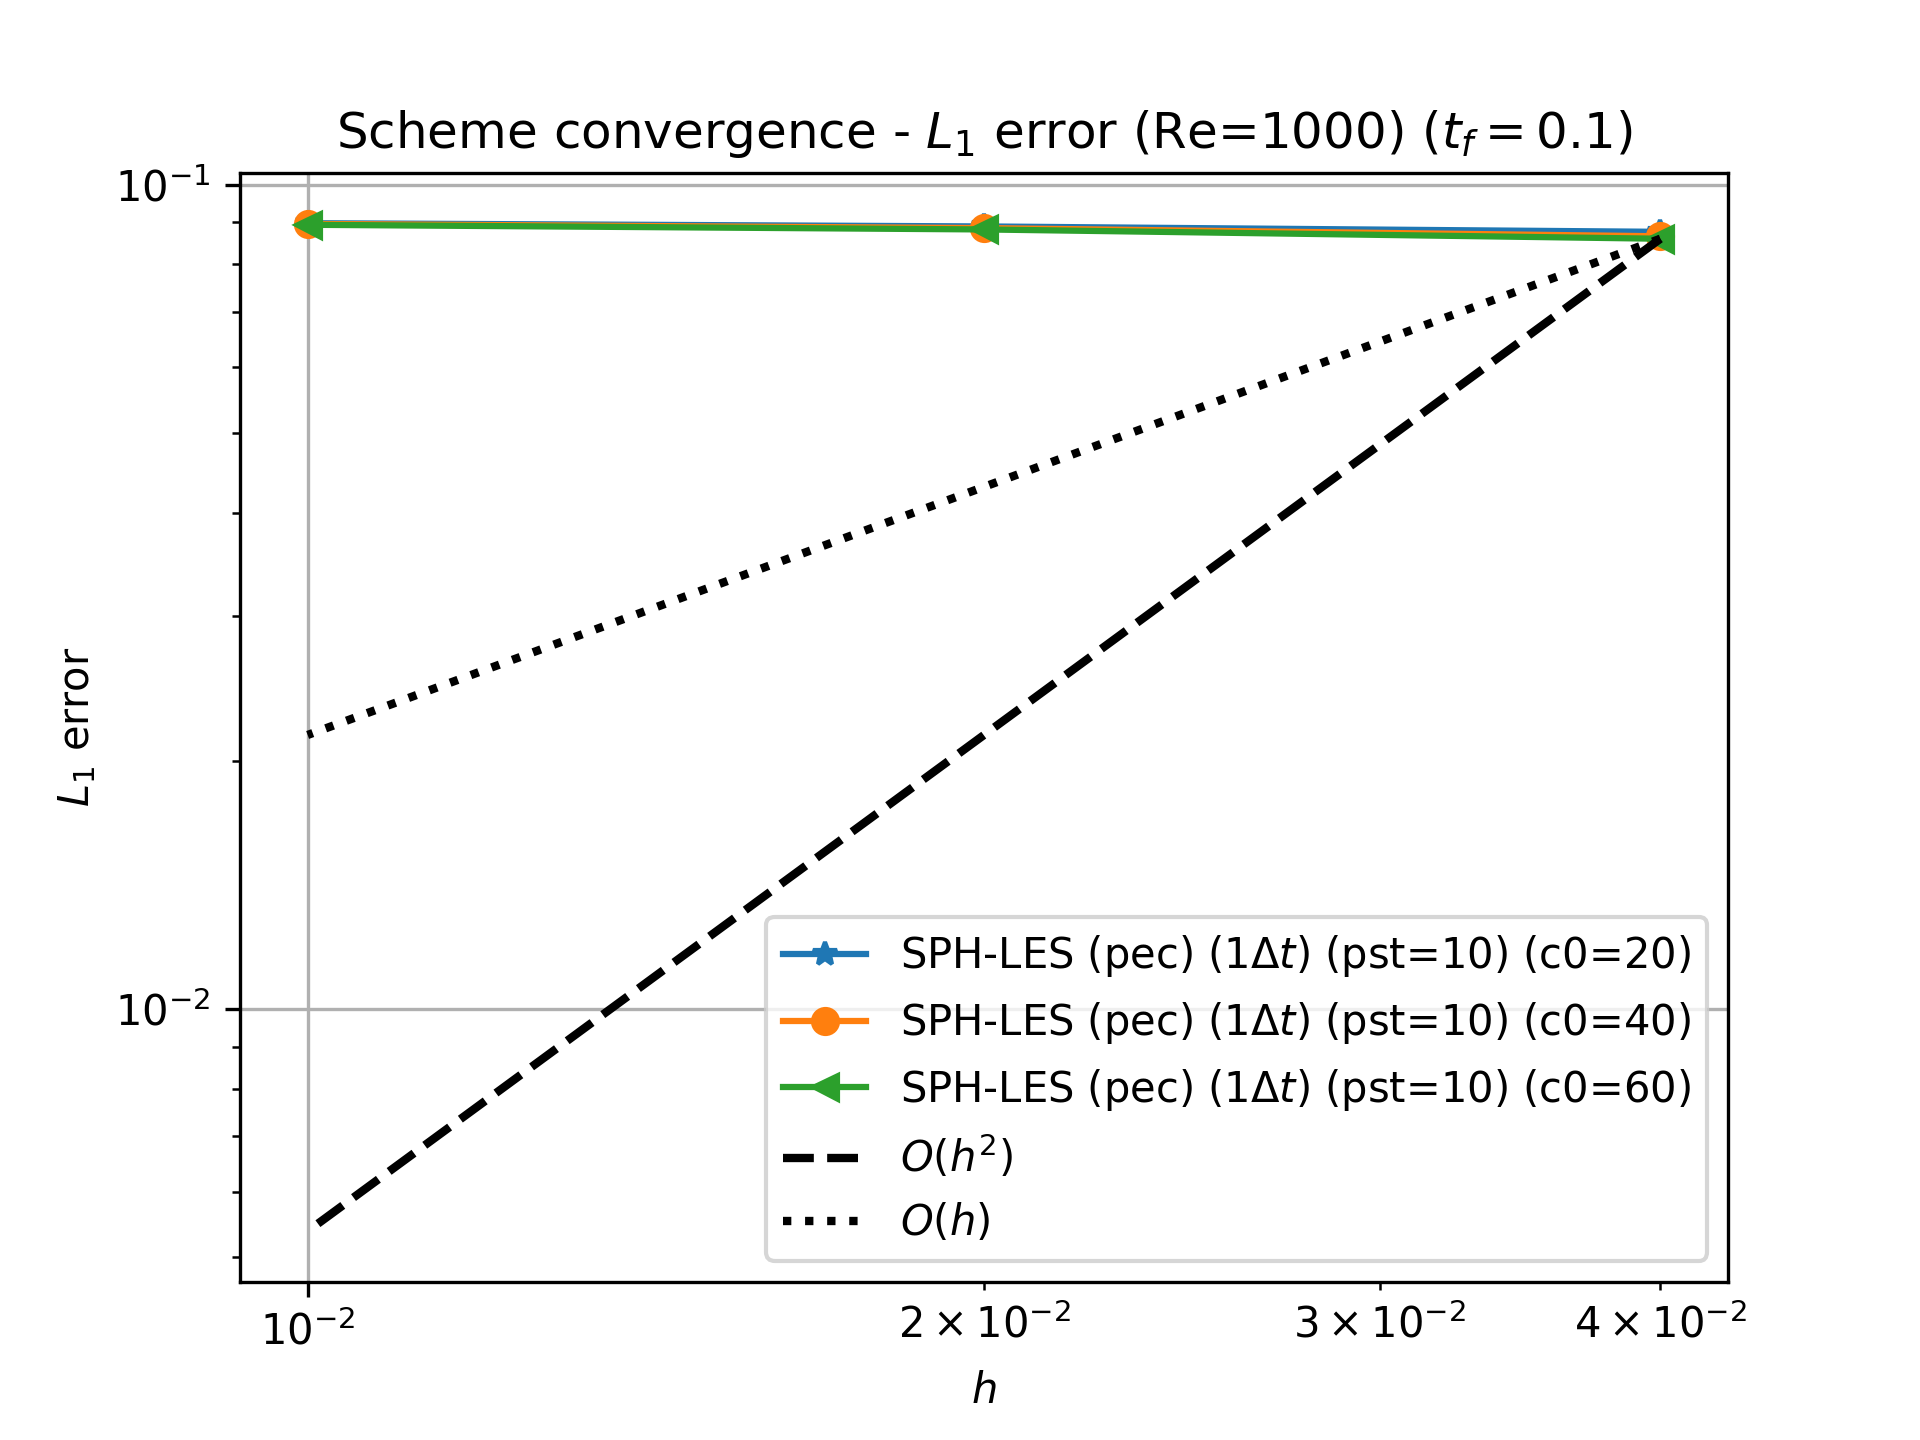
\includegraphics[width=6cm]{Code-Figures/okra2022/c0/dt_pois_conv_c0_pec_re_1000.png}
    \caption{$Re = 1000$}
  \end{subfigure}
  \begin{subfigure}{7cm}
    \centering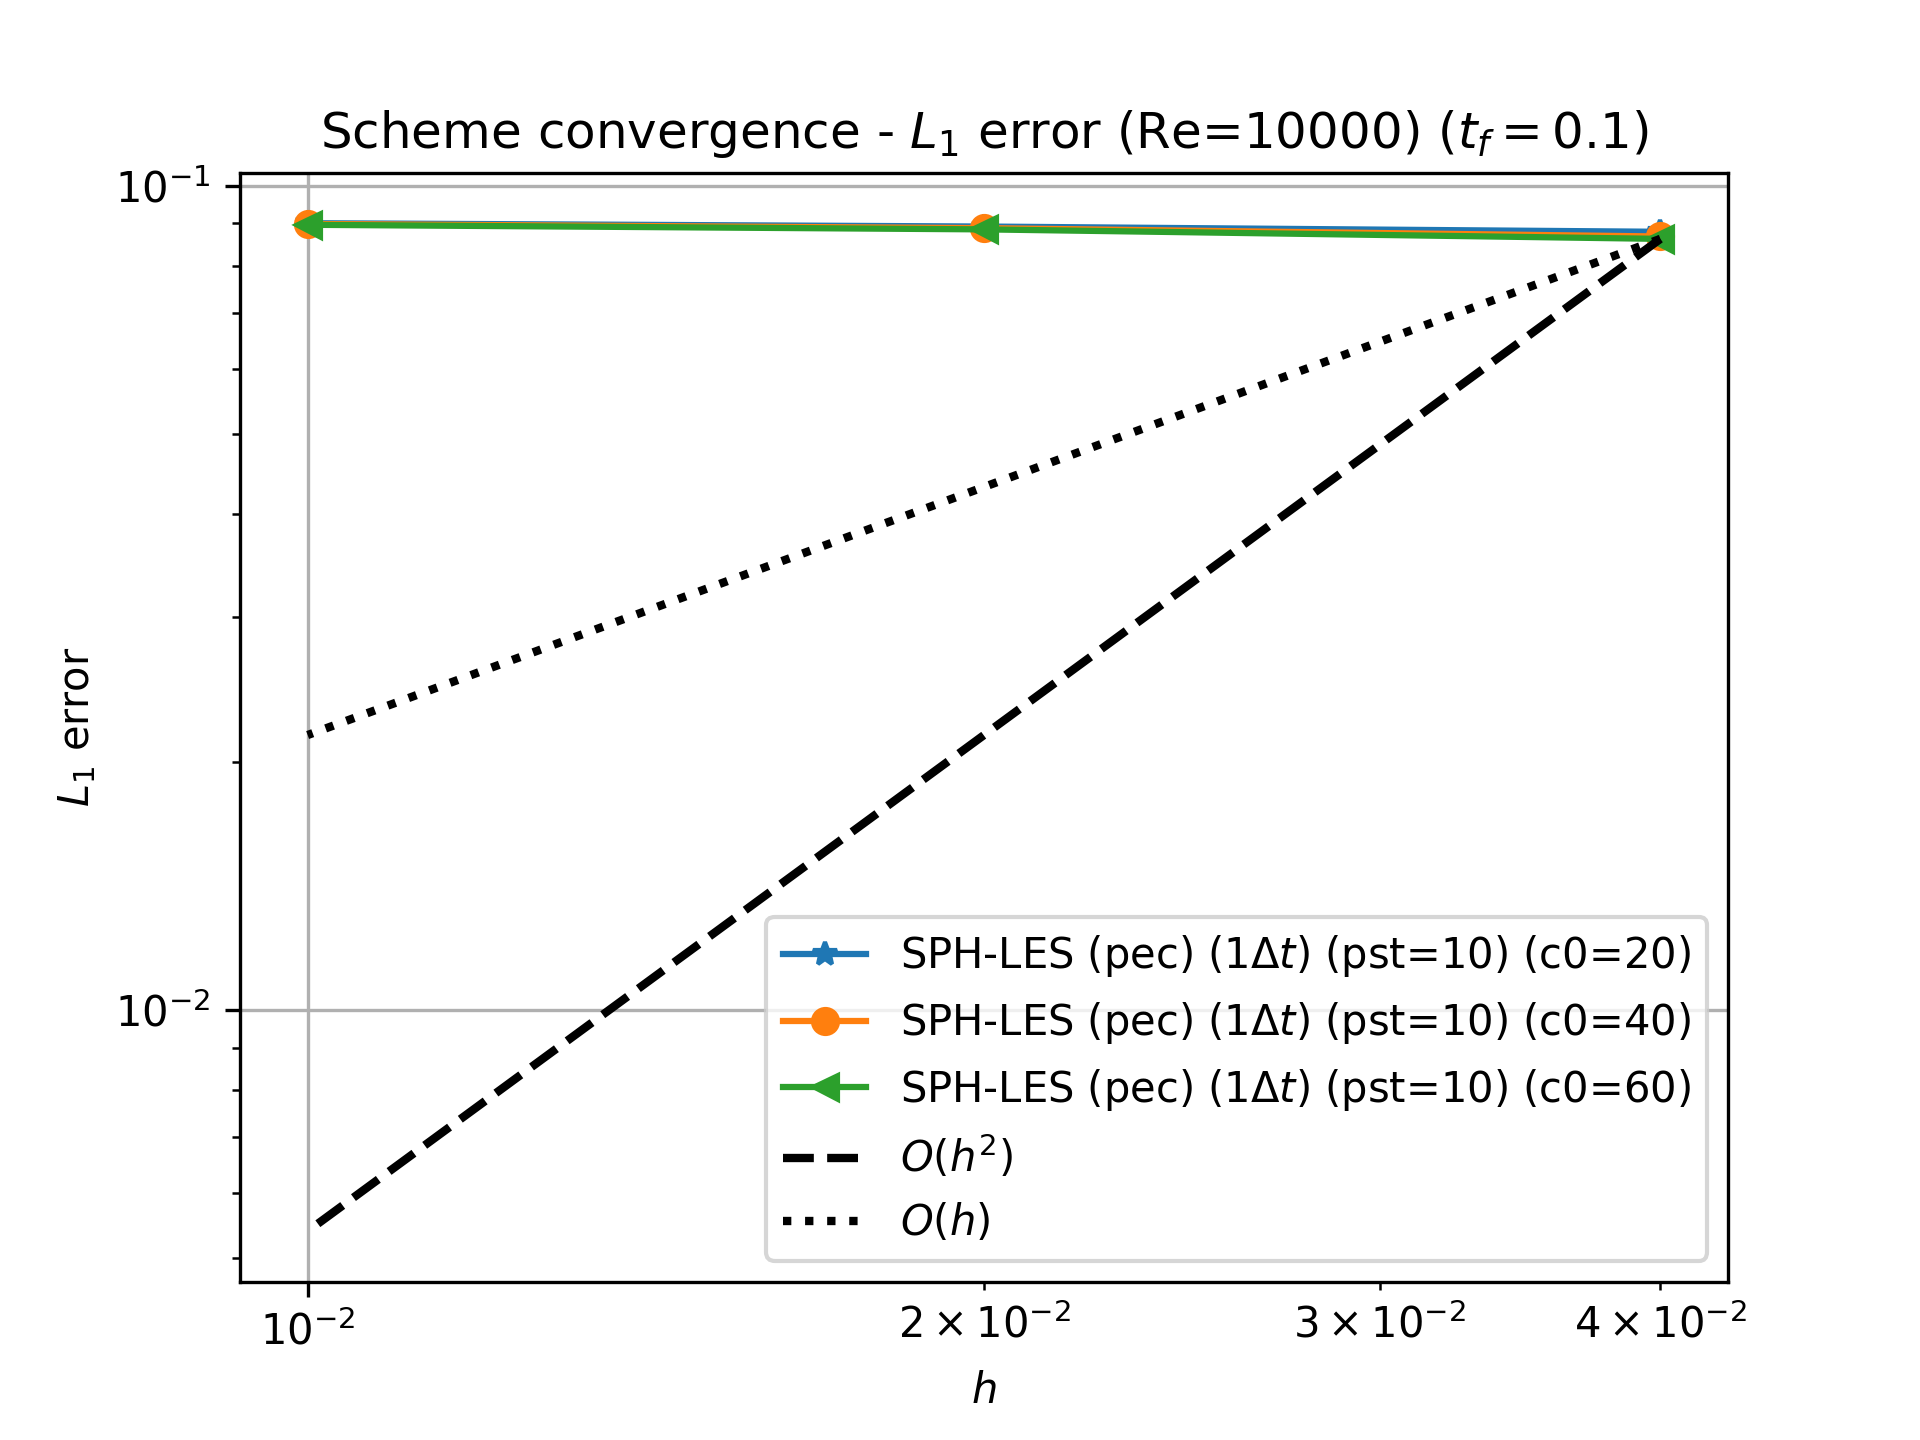
\includegraphics[width=6cm]{Code-Figures/okra2022/c0/dt_pois_conv_c0_pec_re_10000.png}
    \caption{$Re = 10000$}
  \end{subfigure}
  \caption{Convergence of the SPH-LES scheme for various speed of sound values.}
  \label{fig:okra2022-c0}
\end{figure}

In order to test the effect of the speed of sound on the scheme, the following values were considered: $c_s = [20, 40, 60]$. The results are shown in \figref{fig:okra2022-c0}, where it can again be seen that the scheme is zero order convergent, irrespective of the value of $c_s$.
In \figref{fig:okra2022-c0-vmag}, it can be observed that the higher $c_s$ values, which lead to smaller $\Delta t$ values, lead to a more uniformly distributed group of particles, while also leading to an increased $\abs{\vect{v}}_{max}$ value. This seems to add credence to the fact that increasing the resolution in the time domain is dumping additional energy into the system as noise. This is also reflected in the energy spectrum shown in \figref{fig:okra2022-c0-espec}, where it can be observed that the slope of the energy spectrum increases with increasing values of $c_s$.
Therefore, a value of $c_s = 20$ is chosen as the default value for the speed of sound, with the caveat that this scheme possibly cannot be used for problems of lower $Re$ at all since they require dissipation of energy, which does not appear to be the case for this scheme.

\begin{figure}[htbp!]
  \begin{subfigure}{7cm}
    \centering\includegraphics[width=6cm]{Code-Figures/okra2022/c0/c0_20_tait_pec_dtmul_1_nx_50_pst_10_re_10000_ok2022/final_vmag.png}
    \caption{$c_s=20$}
  \end{subfigure}
  \begin{subfigure}{7cm}
    \centering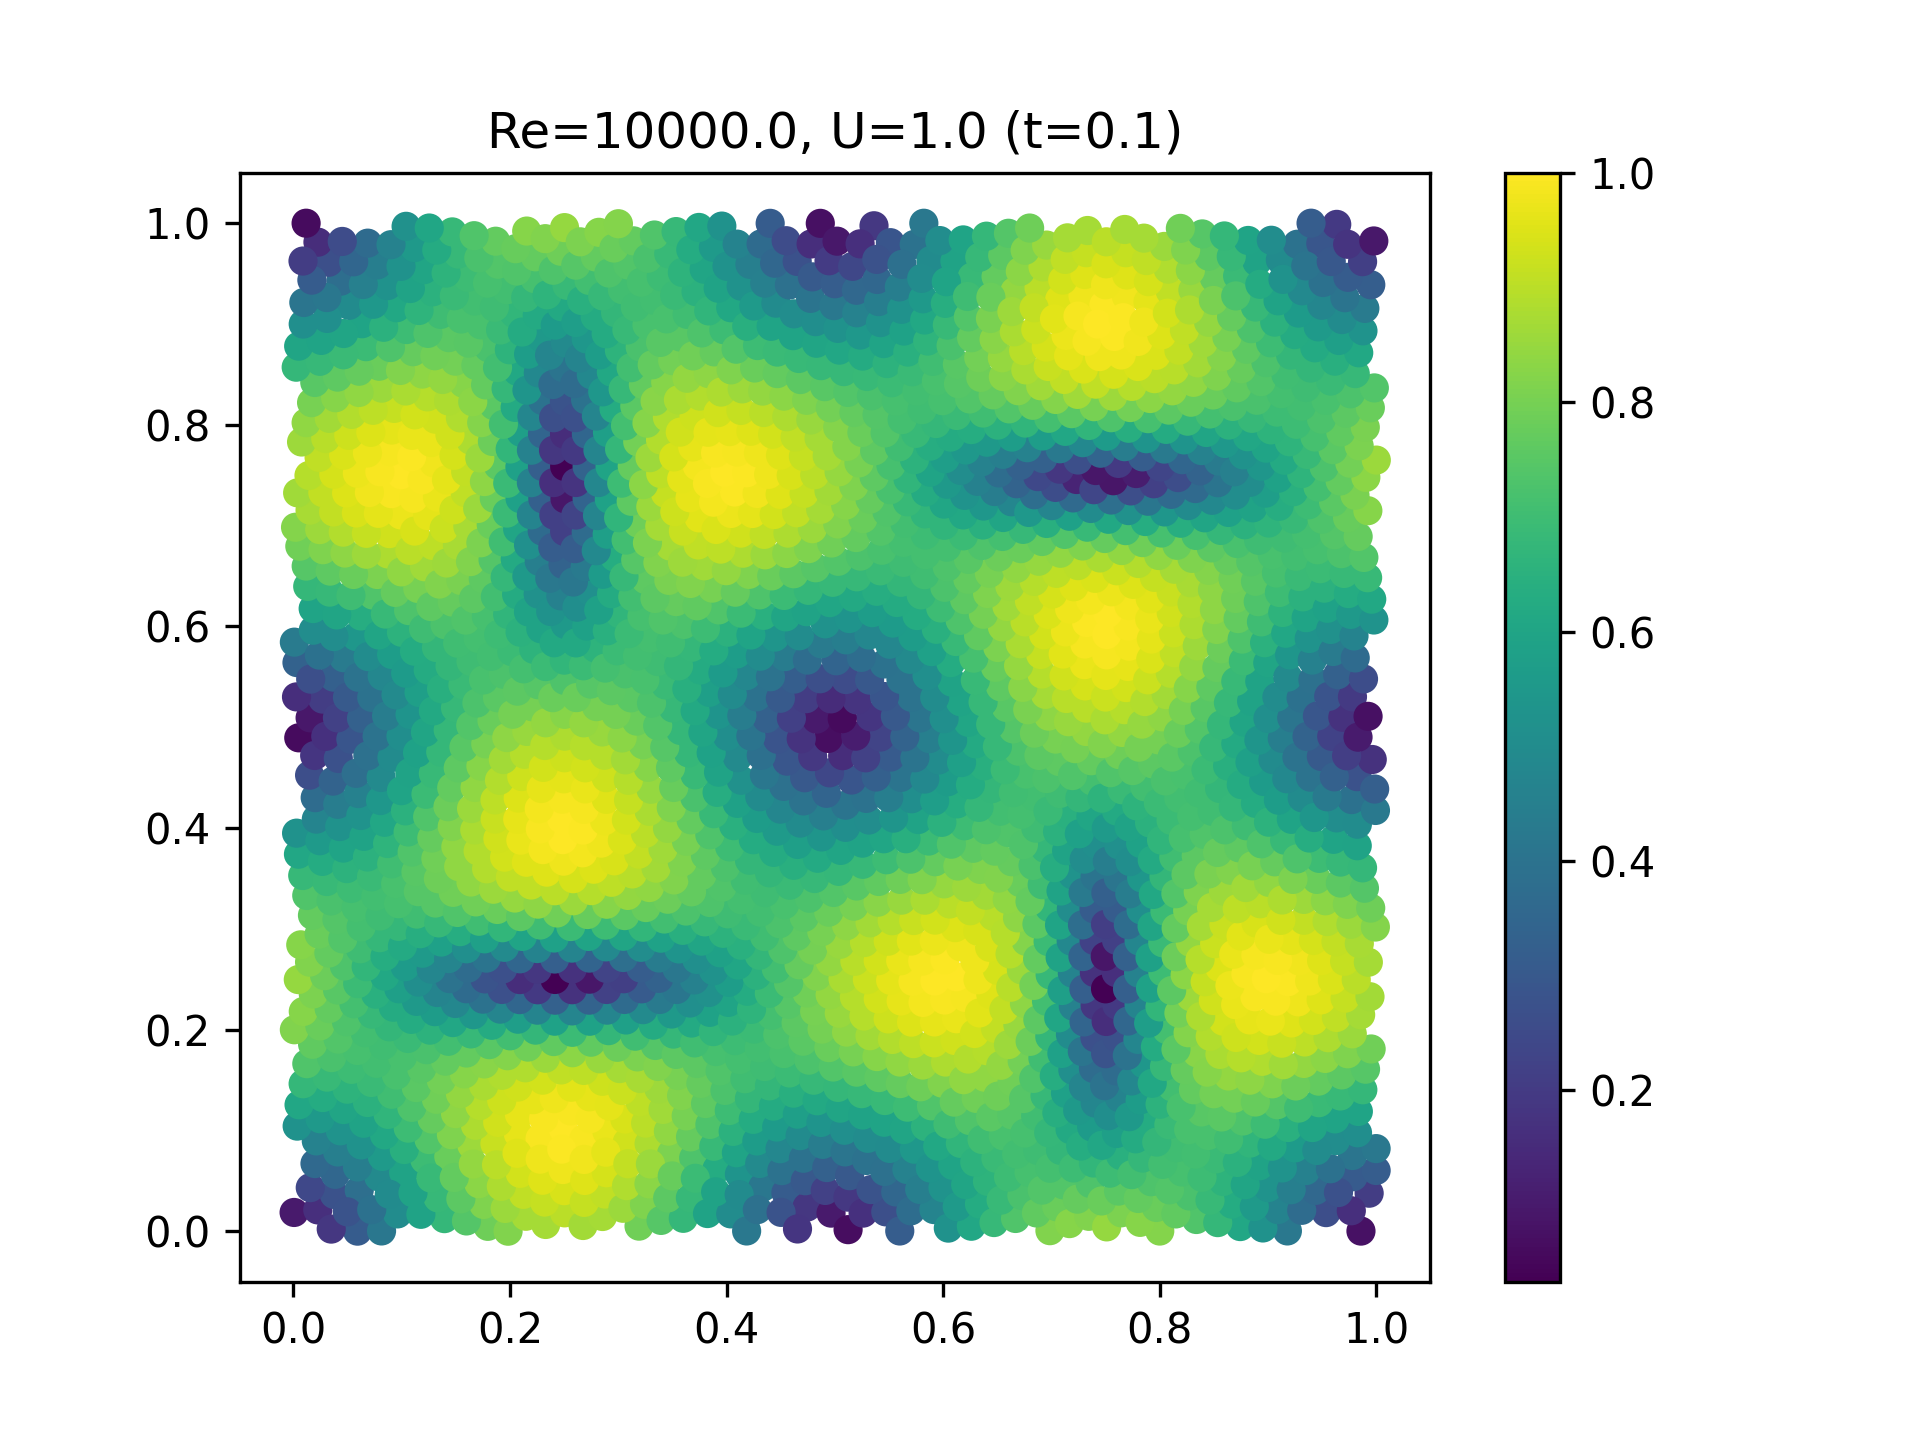
\includegraphics[width=6cm]{Code-Figures/okra2022/c0/c0_40_tait_pec_dtmul_1_nx_50_pst_10_re_10000_ok2022/final_vmag.png}
    \caption{$c_s=40$}
  \end{subfigure}
  \begin{subfigure}{7cm}
    \centering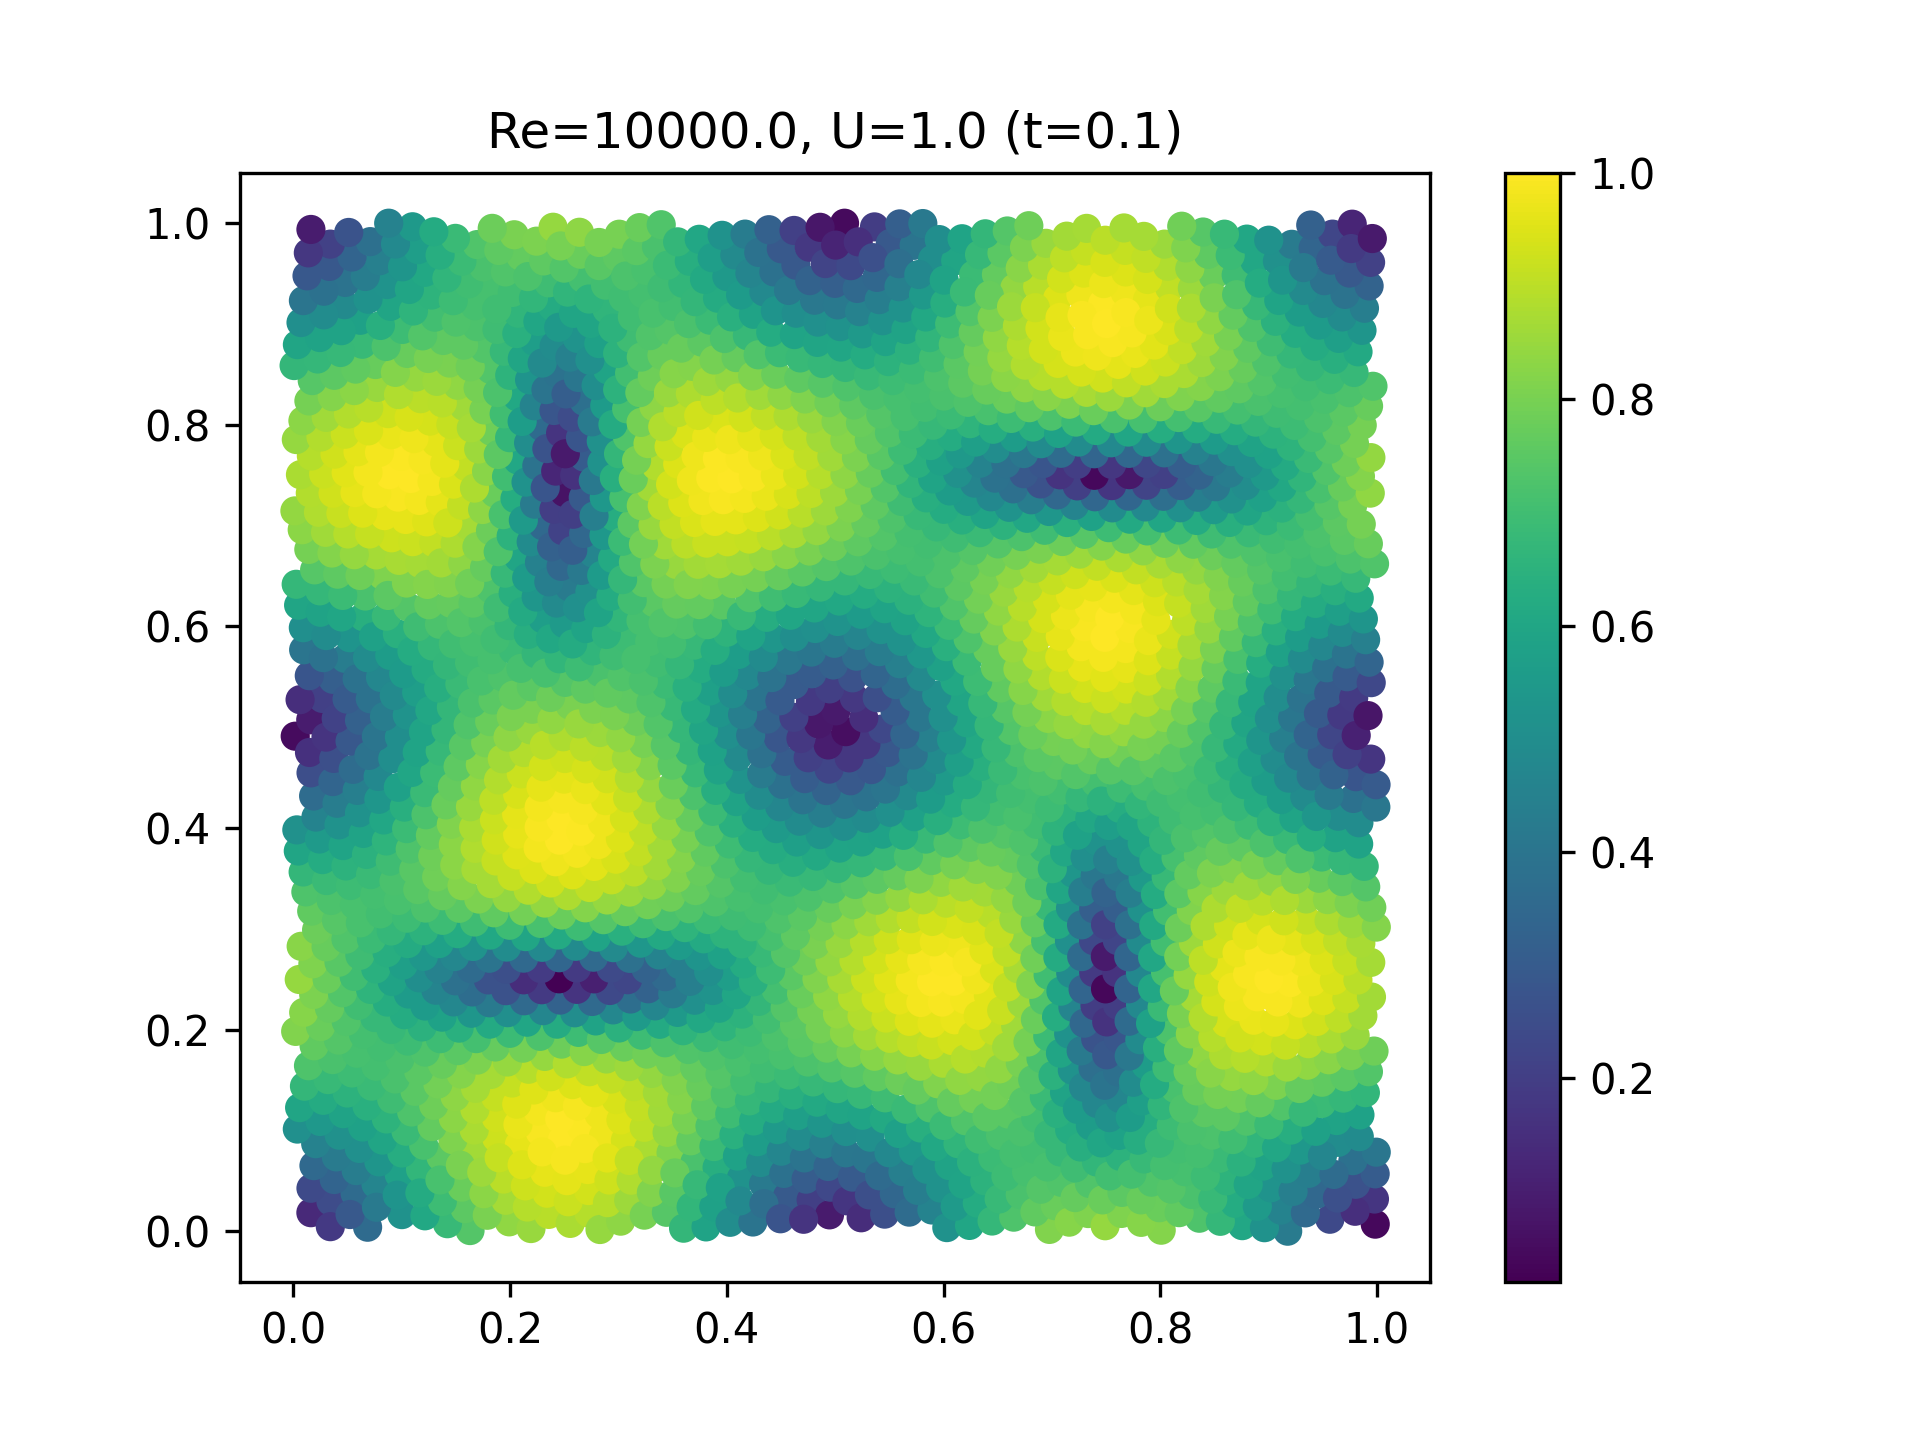
\includegraphics[width=6cm]{Code-Figures/okra2022/c0/c0_60_tait_pec_dtmul_1_nx_50_pst_10_re_10000_ok2022/final_vmag.png}
    \caption{$c_s=60$}
  \end{subfigure}
  \caption{Velocity magnitude field for the SPH-LES scheme for various speed of sound values $(N=50^2, t_f=0.1, Re=10000, f_{pst}=10)$.}
  \label{fig:okra2022-c0-vmag}
\end{figure}

\begin{figure}[htbp!]
  \begin{subfigure}{7cm}
    \centering\includegraphics[width=6cm]{Code-Figures/okra2022/c0/c0_20_tait_pec_dtmul_1_nx_100_pst_10_re_10000_ok2022/energy_spectrum_evolution.png}
    \caption{$c_s=20$}
  \end{subfigure}
  \begin{subfigure}{7cm}
    \centering\includegraphics[width=6cm]{Code-Figures/okra2022/c0/c0_40_tait_pec_dtmul_1_nx_100_pst_10_re_10000_ok2022/energy_spectrum_evolution.png}
    \caption{$c_s=40$}
  \end{subfigure}
  \begin{subfigure}{7cm}
    \centering\includegraphics[width=6cm]{Code-Figures/okra2022/c0/c0_60_tait_pec_dtmul_1_nx_100_pst_10_re_10000_ok2022/energy_spectrum_evolution.png}
    \caption{$c_s=60$}
  \end{subfigure}
  \caption{Evolution of the energy spectrum for the SPH-LES scheme for various speed of sound values $(N=100^2, t_f=0.1, Re=10000, f_{pst}=10)$.}
  \label{fig:okra2022-c0-espec}
\end{figure}

Hence, the SPH-LES scheme is unsuitable for problems of low $Re$ due to the lack of energy dissipation and zero-order convergence. For the cases of high $Re$, the scheme would require much more testing for each specific problem before the computed flow field can be considered accurate. This is reflected in the velocity magnitude plots shown in \figref{fig:okra2022-pst-vmag} and \figref{fig:okra2022-c0-vmag}, where the flow field at the final time instance, is not the expected TGV profile, and instead distorted vortex structures are observed.


\subsection[delta-LES-SPH Scheme]{$\delta$-LES-SPH Scheme}
The Lagrangian LES-based models have only two major schemes to offer. One is the LES-SPH scheme of \cite{DiMascio2017}, and the other is the $\delta$-LES-SPH scheme of \cite{Colagrossi2021QuasiLagrangian}.
The latter was chosen since their scheme introduced a small arbitrary velocity deviation $(\TildeDeltaV)$ to the fluid particles, which allowed for improved accuracy in simulations of high Reynolds number problems. This scheme also included PST and tensile instability control (TIC). This allowed the scheme to tackle the issue of spurious high-frequency noise and the onset of the tensile instability and was hence chosen.

During the scheme's implementation, two choices were made regarding the treatment of the fluid density. The first choice was to note that the fluid density $\rho_c$ is independent of the summation density $\rho$, and in the second choice, both were treated as the same. This was done based on the work of \cite{Negi2022Techniques}, where they observed that the former choice led to improved OOC since the $\rho_c$ should not depend on the particle configuration and should be prescribed with an initial condition. Therefore, these two variants, i.e, $\delta$-LES-SPH $(\rho_c)$ and $\delta$-LES-SPH $(\rho)$, corresponding to the two choices respectively, were considered.

In order to test the influence of the equation of state type on the scheme, the following equations of state were considered:
\begin{itemize}
  \item \texttt{TaitEOS}:
  \begin{equation}
    P_i = P_0 + \frac{\rho_0 c_0^2}{\gamma} \bigg( \Big( \frac{\rho_i}{\rho_0} \Big)^{\gamma} - 1 \bigg),
  \end{equation}

  \item \texttt{LinearEOS}:
  \begin{equation}
    P_i = c_0^2 (\rho_i - \rho_0).
  \end{equation}
\end{itemize}
The results shown in \figref{fig:deltales_sd-eos} and \figref{fig:deltales-eos} highlight clearly that the $\delta$-LES-SPH $(\rho_c)$ implementation with the \texttt{TaitEOS}, clearly offers the best OOC, and hence, is chosen as the default implementation for the $\delta$-LES-SPH scheme.

\begin{figure}[htbp!]
  \begin{subfigure}{7cm}
    \centering\includegraphics[width=6cm]{Code-Figures/deltales_sd/eos/dt_pois_conv_c0_20_re_100.png}
    \caption{$Re = 100$}
  \end{subfigure}
  \begin{subfigure}{7cm}
    \centering\includegraphics[width=6cm]{Code-Figures/deltales_sd/eos/dt_pois_conv_c0_20_re_1000.png}
    \caption{$Re = 1000$}
  \end{subfigure}
  \begin{subfigure}{7cm}
    \centering\includegraphics[width=6cm]{Code-Figures/deltales_sd/eos/dt_pois_conv_c0_20_re_10000.png}
    \caption{$Re = 10000$}
  \end{subfigure}
  \caption{Convergence of the $\delta$-LES-SPH $(\rho)$ scheme for various equations of state.}
  \label{fig:deltales_sd-eos}
\end{figure}

\begin{figure}[htbp!]
  \begin{subfigure}{7cm}
    \centering\includegraphics[width=6cm]{Code-Figures/deltales/eos/dt_pois_conv_c0_20_re_100.png}
    \caption{$Re = 100$}
  \end{subfigure}
  \begin{subfigure}{7cm}
    \centering\includegraphics[width=6cm]{Code-Figures/deltales/eos/dt_pois_conv_c0_20_re_1000.png}
    \caption{$Re = 1000$}
  \end{subfigure}
  \begin{subfigure}{7cm}
    \centering\includegraphics[width=6cm]{Code-Figures/deltales/eos/dt_pois_conv_c0_20_re_10000.png}
    \caption{$Re = 10000$}
  \end{subfigure}
  \caption{Convergence of the $\delta$-LES-SPH $(\rho_c)$ scheme for various equations of state.}
  \label{fig:deltales-eos}
\end{figure}

Subsequently, to test for the effects of the PST on the scheme, multiple values of $f_{pst}$ were considered, and the results are shown in \figref{fig:deltales-pst}.
The trends are hard to decipher here since the magnitude of the error itself is lower for high values of $f_{pst}$ or even without PST, while the OOC is better for lower values of $f_{pst}$.
Therefore, to better analyse these results, the velocity magnitude field and the energy spectrum are plotted in \figref{fig:deltales-pst-vmag} and \figref{fig:deltales-pst-espec} respectively.
Here, it can be observed from the velocity magnitude plot that PST is necessary, particularly with a low $f_{pst}$ value, since without PST, the particles become clustered, and the flow field no longer represents the expected TGV profile.
The energy spectrum plot shows that the energy distribution at the final time instance has barely changed, indicating that the scheme appears to be conservative w.r.t energy, with or without PST. Therefore, long-time studies would be required to ascertain PST's effects on the energy spectrum's evolution.
Hence, for subsequent studies, a value of $f_{pst} = 10$ is chosen as the default value for the PST.

\begin{figure}[htbp!]
  \begin{subfigure}{7cm}
    \centering\includegraphics[width=6cm]{Code-Figures/deltales/pst/dt_pois_conv_c0_20_re_100.png}
    \caption{$Re = 100$}
  \end{subfigure}
  \begin{subfigure}{7cm}
    \centering\includegraphics[width=6cm]{Code-Figures/deltales/pst/dt_pois_conv_c0_20_re_1000.png}
    \caption{$Re = 1000$}
  \end{subfigure}
  \begin{subfigure}{7cm}
    \centering\includegraphics[width=6cm]{Code-Figures/deltales/pst/dt_pois_conv_c0_20_re_10000.png}
    \caption{$Re = 10000$}
  \end{subfigure}
  \caption{Convergence of the $\delta$-LES-SPH $(\rho_c)$ scheme for various $f_{pst}$ values.}
  \label{fig:deltales-pst}
\end{figure}

\begin{figure}[htbp!]
  \begin{subfigure}{7cm}
    \centering\includegraphics[width=6cm]{Code-Figures/deltales/pst/c0_20_tait_pec_dtmul_1_nx_50_pst_-1_re_10000_deltales/final_vmag.png}
    \caption{No PST}
  \end{subfigure}
  \begin{subfigure}{7cm}
    \centering\includegraphics[width=6cm]{Code-Figures/deltales/pst/c0_20_tait_pec_dtmul_1_nx_50_pst_10_re_10000_deltales/final_vmag.png}
    \caption{$f_{pst} = 10$}
  \end{subfigure}
  \begin{subfigure}{7cm}
    \centering\includegraphics[width=6cm]{Code-Figures/deltales/pst/c0_20_tait_pec_dtmul_1_nx_50_pst_50_re_10000_deltales/final_vmag.png}
    \caption{$f_{pst} = 50$}
  \end{subfigure}
  \begin{subfigure}{7cm}
    \centering\includegraphics[width=6cm]{Code-Figures/deltales/pst/c0_20_tait_pec_dtmul_1_nx_50_pst_100_re_10000_deltales/final_vmag.png}
    \caption{$f_{pst} = 100$}
  \end{subfigure}
  \caption{Velocity magnitude field for the $\delta$-LES-SPH $(\rho_c)$ scheme for various $f_{pst}$ values $(N=50^2, t_f=0.1, Re=10000, c_s=20)$.}
  \label{fig:deltales-pst-vmag}
\end{figure}

\begin{figure}[htbp!]
  \begin{subfigure}{7cm}
    \centering\includegraphics[width=6cm]{Code-Figures/deltales/pst/c0_20_tait_pec_dtmul_1_nx_100_pst_-1_re_10000_deltales/energy_spectrum_evolution.png}
    \caption{No PST}
  \end{subfigure}
  \begin{subfigure}{7cm}
    \centering\includegraphics[width=6cm]{Code-Figures/deltales/pst/c0_20_tait_pec_dtmul_1_nx_100_pst_10_re_10000_deltales/energy_spectrum_evolution.png}
    \caption{$f_{pst} = 10$}
  \end{subfigure}
  \begin{subfigure}{7cm}
    \centering\includegraphics[width=6cm]{Code-Figures/deltales/pst/c0_20_tait_pec_dtmul_1_nx_100_pst_50_re_10000_deltales/energy_spectrum_evolution.png}
    \caption{$f_{pst} = 50$}
  \end{subfigure}
  \begin{subfigure}{7cm}
    \centering\includegraphics[width=6cm]{Code-Figures/deltales/pst/c0_20_tait_pec_dtmul_1_nx_100_pst_100_re_10000_deltales/energy_spectrum_evolution.png}
    \caption{$f_{pst} = 100$}
  \end{subfigure}
  \caption{Evolution of the energy spectrum for the $\delta$-LES-SPH $(\rho_c)$ scheme for various $f_{pst}$ values $(N=100^2, t_f=0.1, Re=10000, c_s=20)$. The initial energy spectrum is plotted in dark blue, and the final energy spectrum is plotted in yellow.}
  \label{fig:deltales-pst-espec}
\end{figure}

The original scheme of \cite{Colagrossi2021QuasiLagrangian} used a \texttt{RK4} time-integrator with a $CFL=1.5$. Therefore, to study the effects of the time-integrator, the following schemes were considered: \texttt{PEC}, \texttt{RK2} and \texttt{RK4}, with an appropriate $CFL$ value for each scheme. The results are shown in \figref{fig:deltales-integrator}, where it can be observed that the \texttt{RK2} scheme offers the best OOC and hence, is chosen as the default time-integrator for the $\delta$-LES-SPH scheme. It is also to be noted that the \texttt{RK2} integrator is also the fastest, as shown in \figref{fig:deltales-integrator-rt}, while offering a speedup of $\approx 1.6$ times over the \texttt{RK4} integrator.
It is also noted that there are no significant differences to be observed in the velocity magnitude field and the energy spectrum, as shown in \figref{fig:deltales-integrator-vmag} and \figref{fig:deltales-integrator-espec} respectively, for the different time-integrators.

\begin{figure}[htbp!]
  \begin{subfigure}{7cm}
    \centering\includegraphics[width=6cm]{Code-Figures/deltales/integrator/dt_pois_conv_c0_20_re_100.png}
    \caption{$Re = 100$}
  \end{subfigure}
  \begin{subfigure}{7cm}
    \centering\includegraphics[width=6cm]{Code-Figures/deltales/integrator/dt_pois_conv_c0_20_re_1000.png}
    \caption{$Re = 1000$}
  \end{subfigure}
  \begin{subfigure}{7cm}
    \centering\includegraphics[width=6cm]{Code-Figures/deltales/integrator/dt_pois_conv_c0_20_re_10000.png}
    \caption{$Re = 10000$}
  \end{subfigure}
  \caption{Convergence of the $\delta$-LES-SPH $(\rho_c)$ scheme for various time-integrators.}
  \label{fig:deltales-integrator}
\end{figure}

\begin{figure}[htbp!]
  \begin{subfigure}{7cm}
    \centering\includegraphics[width=6cm]{Code-Figures/deltales/integrator/pois_rt_pst_10_c0_20_re_100.png}
    \caption{$Re = 100$}
  \end{subfigure}
  \begin{subfigure}{7cm}
    \centering\includegraphics[width=6cm]{Code-Figures/deltales/integrator/pois_rt_pst_10_c0_20_re_1000.png}
    \caption{$Re = 1000$}
  \end{subfigure}
  \begin{subfigure}{7cm}
    \centering\includegraphics[width=6cm]{Code-Figures/deltales/integrator/pois_rt_pst_10_c0_20_re_10000.png}
    \caption{$Re = 10000$}
  \end{subfigure}
  \caption{Run-time (in $s$) of the $\delta$-LES-SPH $(\rho_c)$ scheme for various time-integrators.}
  \label{fig:deltales-integrator-rt}
\end{figure}

\begin{figure}[htbp!]
  \begin{subfigure}{7cm}
    \centering\includegraphics[width=6cm]{Code-Figures/deltales/integrator/c0_20_tait_pec_dtmul_1_nx_50_pst_10_re_10000_deltales/final_vmag.png}
    \caption{\texttt{PEC}}
  \end{subfigure}
  \begin{subfigure}{7cm}
    \centering\includegraphics[width=6cm]{Code-Figures/deltales/integrator/c0_20_tait_rk2_dtmul_1.5_nx_50_pst_10_re_10000_deltales/final_vmag.png}
    \caption{\texttt{RK2}}
  \end{subfigure}
  \begin{subfigure}{7cm}
    \centering\includegraphics[width=6cm]{Code-Figures/deltales/integrator/c0_20_tait_rk4_dtmul_2_nx_50_pst_10_re_10000_deltales/final_vmag.png}
    \caption{\texttt{RK4}}
  \end{subfigure}
  \caption{Velocity magnitude field for the $\delta$-LES-SPH $(\rho_c)$ scheme for various time-integrators $(N=50^2, t_f=0.1, Re=10000, c_s=20, f_{pst}=10)$.}
  \label{fig:deltales-integrator-vmag}
\end{figure}

\begin{figure}[htbp!]
  \begin{subfigure}{7cm}
    \centering\includegraphics[width=6cm]{Code-Figures/deltales/integrator/c0_20_tait_pec_dtmul_1_nx_100_pst_10_re_10000_deltales/energy_spectrum_evolution.png}
    \caption{\texttt{PEC}}
  \end{subfigure}
  \begin{subfigure}{7cm}
    \centering\includegraphics[width=6cm]{Code-Figures/deltales/integrator/c0_20_tait_rk2_dtmul_1.5_nx_100_pst_10_re_10000_deltales/energy_spectrum_evolution.png}
    \caption{\texttt{RK2}}
  \end{subfigure}
  \begin{subfigure}{7cm}
    \centering\includegraphics[width=6cm]{Code-Figures/deltales/integrator/c0_20_tait_rk4_dtmul_2_nx_100_pst_10_re_10000_deltales/energy_spectrum_evolution.png}
    \caption{\texttt{RK4}}
  \end{subfigure}
  \caption{Evolution of the energy spectrum for the $\delta$-LES-SPH $(\rho_c)$ scheme for various time-integrators $(N=100^2, t_f=0.1, Re=10000, c_s=20, f_{pst}=10)$.}
  \label{fig:deltales-integrator-espec}
\end{figure}



\subsection[k-epsilon SPH Scheme]{$k-\epsilon$ SPH Scheme}
The $k-\epsilon$ SPH scheme of \cite{Shao2006} was chosen over the other RANS-based schemes since the authors considered the typical RANS-based $k-\epsilon$ equations, as the governing equations for their scheme, with an implicit pressure Poisson equation that needed to be solved for the time integration of the scheme.
However, it was decided that since such an implicit pressure Poisson equation solver would be computationally expensive, as well as complicated to general to other problems, the scheme was implemented with a different SPH discretisation of the $k-\epsilon$ transport equations to avoid that step.

Therefore, two choices were available when it came to discretising the $k-\epsilon$ transport equations.
The first would involve discretising the original $k-\epsilon$ equations as detailed below:
\begin{equation}
  \LagDerivative{k} = \nabla \cdot \bigg( \frac{\nu_t}{\sigma_k} \nabla k \bigg) + P_k - \epsilon,
  \label{eq:Shao2006-k-transport-eq-res-chap}
\end{equation}
\begin{equation}
  \LagDerivative{\epsilon} = \nabla \cdot \bigg( \frac{\nu_t}{\sigma_{\epsilon}} \nabla \epsilon \bigg) + c_{1\epsilon} \frac{\epsilon}{k} P_k - c_{2\epsilon} \frac{\epsilon^2}{k}.
  \label{eq:Shao2006-eps-transport-eq-res-chap}
\end{equation}
Alternatively, the above equations can also be expanded, using standard identities from calculus and substituting for the turbulent eddy viscosity $\nu_t$ to obtain:
\begin{equation}
  \LagDerivative{k} = \frac{c_d}{\sigma_k} \bigg( \frac{k^2}{\epsilon} \nabla^2 k + \frac{2k}{\epsilon} (\nabla k)^2 - \frac{k^2}{\epsilon^2} \nabla k \cdot \nabla \epsilon \bigg) + P_k - \epsilon,
  \label{eq:Shao2006-k-transport-eq-exp-res-chap}
\end{equation}
\begin{equation}
  \LagDerivative{\epsilon} = \frac{c_d}{\sigma_\epsilon} \bigg( \frac{k^2}{\epsilon} \nabla^2 \epsilon + \frac{2k}{\epsilon} \nabla k \cdot \nabla \epsilon - \frac{k^2}{\epsilon^2} (\nabla \epsilon)^2 \bigg) + c_{1\epsilon} \frac{\epsilon}{k} P_k - c_{2\epsilon} \frac{\epsilon^2}{k}.
  \label{eq:Shao2006-eps-transport-eq-exp-res-chap}
\end{equation}

Therefore, the two variants, i.e., $k-\epsilon$ simplified and $k-\epsilon$ expanded, corresponding to the two choices for the pair of transport equations are discretised using SOC SPH operators as detailed in the work of \cite{Negi2022Techniques}.
In order to verify the correctness of the SPH discretisation of the $k-\epsilon$ transport equations, in either case, and study the OOC of the transport equations, a single time-step of the scheme was run on a predetermined set of initial conditions for the flow properties, including $k$ and $\epsilon$. The computed RHS of the $k$ and $\epsilon$ transport equations were then compared with the analytical RHS of the equations, and the appropriate $L_1$ error was computed and plotted for various resolutions.
Three test cases were devised to represent three distinct functional forms. Flow properties such as the velocity, pressure and density were modelled after the initial conditions of the $2D$ TGV problem, as detailed in \secref{sec:taylor-green-vortex-problem}. In contrast, the initial conditions for $k$ and $\epsilon$ fields were defined as follows:
\begin{itemize}
  \item \texttt{Test-case 1}:
  \begin{equation}
    k_0 = 1.5 U^2, \quad \epsilon_0 = 0.09^{0.75} \frac{k_0^{1.5}}{L},
  \end{equation}
  where $U$ and $L$ are the characteristic velocity and length scales. This test case represents a constant and uniform initial condition for the $k-\epsilon$ fields.

  \item \texttt{Test-case 2}:
  \begin{equation}
    k_0 = \abs{\vect{v}_0}^2, \quad \epsilon_0 = k_0,
  \end{equation}
  where $\vect{v}_0$ is the initial velocity field. This test case represents a $k-\epsilon$ field proportional to the velocity field.

  \item \texttt{Test-case 3}:
  \begin{equation}
    k_0 = \frac{1}{2}\abs{\vect{v}_0}^2, \quad \epsilon_0 = 0.09 \frac{k_0^{3/2}}{L}.
  \end{equation}
  This test case represents a $k-\epsilon$ field that is non-linearly proportional to the velocity field.
\end{itemize}
For all of the above cases, the analytical values of the RHS of the $k$ and $\epsilon$ transport equations are computed using \texttt{SymPy} \parencite{Meurer2017}, a symbolic package in order to automate the process and avoid any errors in the analytical computation.

The results for the $k$ and $\epsilon$ transport equations are shown in \figref{fig:k-spatial-ooc} and \figref{fig:eps-spatial-ooc} respectively. It can be observed here that for the first test case, the OOC for the spatial operators in the transport equation agrees well, irrespective of the variant of discretisation.
However, the $k-\epsilon$ simplified variant in the subsequent test cases shows a better OOC than the $k-\epsilon$ expanded variant.
This can be attributed to the fact that in the expanded equations of \eqref{eq:Shao2006-k-transport-eq-exp-res-chap} and \eqref{eq:Shao2006-eps-transport-eq-exp-res-chap}, the terms involve either higher-order derivatives or products of derivatives, which are not well approximated by the SPH operators, and hence, lead to increased errors. It appears that the advantage of dealing with single-term derivatives (e.g., $\nabla k$) in the expanded equations, compared to having multi-term derivatives (e.g., $\nabla \cdot (k^2\nabla k / \epsilon)$) in the simplified equations, is not enough to offset the increased numerical errors due to the higher-order derivatives.
This is also made more evident in the actual $k-\epsilon$ fields, as shown in \figref{fig:k-spatial-ooc-field} and \figref{fig:eps-spatial-ooc-field}, respectively.
Therefore, the $k-\epsilon$ simplified variant is chosen as the default variant for the $k-\epsilon$ SPH scheme.

\begin{figure}[htbp!]
  \begin{subfigure}{7cm}
    \centering\includegraphics[width=6cm]{Code-Figures/keps/keps-op-conv/k_conv_tc_1_re_10000.png}
    \caption{Test-case 1}
  \end{subfigure}
  \begin{subfigure}{7cm}
    \centering\includegraphics[width=6cm]{Code-Figures/keps/keps-op-conv/k_conv_tc_2_re_10000.png}
    \caption{Test-case 2}
  \end{subfigure}
  \begin{subfigure}{7cm}
    \centering\includegraphics[width=6cm]{Code-Figures/keps/keps-op-conv/k_conv_tc_3_re_10000.png}
    \caption{Test-case 3}
  \end{subfigure}
  \caption{Convergence of the spatial operators in the $k$ transport equation for various test-cases.}
  \label{fig:k-spatial-ooc}
\end{figure}

\begin{figure}[htbp!]
  \begin{subfigure}{7cm}
    \centering\includegraphics[width=6cm]{Code-Figures/keps/keps-op-conv/eps_conv_tc_1_re_10000.png}
    \caption{Test-case 1}
  \end{subfigure}
  \begin{subfigure}{7cm}
    \centering\includegraphics[width=6cm]{Code-Figures/keps/keps-op-conv/eps_conv_tc_2_re_10000.png}
    \caption{Test-case 2}
  \end{subfigure}
  \begin{subfigure}{7cm}
    \centering\includegraphics[width=6cm]{Code-Figures/keps/keps-op-conv/eps_conv_tc_3_re_10000.png}
    \caption{Test-case 3}
  \end{subfigure}
  \caption{Convergence of the spatial operators in the $\epsilon$ transport equation for various test-cases.}
  \label{fig:eps-spatial-ooc}
\end{figure}

\begin{figure}[htbp!]
  \begin{subfigure}{7cm}
    \centering\includegraphics[width=6cm]{Code-Figures/keps/keps-op-conv/c0_60_ke_expd_no_ketc_1_nx_150_re_10000/k_rhs.png}
    \caption{Test-case 1, Simplified $k$}
  \end{subfigure}
  \begin{subfigure}{7cm}
    \centering\includegraphics[width=6cm]{Code-Figures/keps/keps-op-conv/c0_60_ke_expd_yes_ketc_1_nx_150_re_10000/k_rhs.png}
    \caption{Test-case 1, Expanded $k$}
  \end{subfigure}
  \begin{subfigure}{7cm}
    \centering\includegraphics[width=6cm]{Code-Figures/keps/keps-op-conv/c0_60_ke_expd_no_ketc_2_nx_150_re_10000/k_rhs.png}
    \caption{Test-case 2, Simplified $k$}
  \end{subfigure}
  \begin{subfigure}{7cm}
    \centering\includegraphics[width=6cm]{Code-Figures/keps/keps-op-conv/c0_60_ke_expd_yes_ketc_2_nx_150_re_10000/k_rhs.png}
    \caption{Test-case 2, Expanded $k$}
  \end{subfigure}
  \begin{subfigure}{7cm}
    \centering\includegraphics[width=6cm]{Code-Figures/keps/keps-op-conv/c0_60_ke_expd_no_ketc_3_nx_150_re_10000/k_rhs.png}
    \caption{Test-case 3, Simplified $k$}
  \end{subfigure}
  \begin{subfigure}{7cm}
    \centering\includegraphics[width=6cm]{Code-Figures/keps/keps-op-conv/c0_60_ke_expd_yes_ketc_3_nx_150_re_10000/k_rhs.png}
    \caption{Test-case 3, Expanded $k$}
  \end{subfigure}
  \caption{RHS of the $k$ transport equation for various test-cases $(N=150^2, t_f=1\Delta t, Re=10000, c_s=60)$.}
  \label{fig:k-spatial-ooc-field}
\end{figure}

\begin{figure}[htbp!]
  \begin{subfigure}{7cm}
    \centering\includegraphics[width=6cm]{Code-Figures/keps/keps-op-conv/c0_60_ke_expd_no_ketc_1_nx_150_re_10000/eps_rhs.png}
    \caption{Test-case 1, Simplified $\epsilon$}
  \end{subfigure}
  \begin{subfigure}{7cm}
    \centering\includegraphics[width=6cm]{Code-Figures/keps/keps-op-conv/c0_60_ke_expd_yes_ketc_1_nx_150_re_10000/eps_rhs.png}
    \caption{Test-case 1, Expanded $\epsilon$}
  \end{subfigure}
  \begin{subfigure}{7cm}
    \centering\includegraphics[width=6cm]{Code-Figures/keps/keps-op-conv/c0_60_ke_expd_no_ketc_2_nx_150_re_10000/eps_rhs.png}
    \caption{Test-case 2, Simplified $\epsilon$}
  \end{subfigure}
  \begin{subfigure}{7cm}
    \centering\includegraphics[width=6cm]{Code-Figures/keps/keps-op-conv/c0_60_ke_expd_yes_ketc_2_nx_150_re_10000/eps_rhs.png}
    \caption{Test-case 2, Expanded $\epsilon$}
  \end{subfigure}
  \begin{subfigure}{7cm}
    \centering\includegraphics[width=6cm]{Code-Figures/keps/keps-op-conv/c0_60_ke_expd_no_ketc_3_nx_150_re_10000/eps_rhs.png}
    \caption{Test-case 3, Simplified $\epsilon$}
  \end{subfigure}
  \begin{subfigure}{7cm}
    \centering\includegraphics[width=6cm]{Code-Figures/keps/keps-op-conv/c0_60_ke_expd_yes_ketc_3_nx_150_re_10000/eps_rhs.png}
    \caption{Test-case 3, Expanded $\epsilon$}
  \end{subfigure}
  \caption{RHS of the $\epsilon$ transport equation for various test-cases $(N=150^2, t_f=1\Delta t, Re=10000, c_s=60)$.}
  \label{fig:eps-spatial-ooc-field}
\end{figure}


In order to study the effects of the various equations of state on the, the convergence study was performed on the $k-\epsilon$ SPH scheme, involving the SPH discretisation of simplified $k-\epsilon$ transport equations, and the \texttt{PEC} time-integrator.
The results are shown in \figref{fig:keps-eos}, where it can be observed that both the \texttt{LinearEOS} and \texttt{TaitEOS} appear to offer zeroth-order convergence.
To gain further insight, \figref{fig:keps-eos-vmag} and \figref{fig:keps-eos-espec} are referred to, where it can be observed that the velocity field computed using the \texttt{TaitEOS} appears to better correspond to the typical TGV profile.
The energy spectrum is interesting because the \texttt{LinearEOS} appears to redistribute energy from the larger to smaller scales. In contrast, the \texttt{TaitEOS} appears to dissipate energy in the system for all scales.
Although the former behaviour is more desirable, as it is more representative of the physical system, the actual velocity field plot for the \texttt{LinearEOS} scheme indicates its instability, and hence, the \texttt{TaitEOS} is chosen as the default equation of state for the $k-\epsilon$ SPH scheme.

\begin{figure}[htbp!]
  \begin{subfigure}{7cm}
    \centering\includegraphics[width=6cm]{Code-Figures/keps/eos/dt_pois_conv_c0_20_re_100.png}
    \caption{$Re = 100$}
  \end{subfigure}
  \begin{subfigure}{7cm}
    \centering\includegraphics[width=6cm]{Code-Figures/keps/eos/dt_pois_conv_c0_20_re_1000.png}
    \caption{$Re = 1000$}
  \end{subfigure}
  \begin{subfigure}{7cm}
    \centering\includegraphics[width=6cm]{Code-Figures/keps/eos/dt_pois_conv_c0_20_re_10000.png}
    \caption{$Re = 10000$}
  \end{subfigure}
  \caption{Convergence of the $k-\epsilon$ SPH scheme for various equations of state.}
  \label{fig:keps-eos}
\end{figure}

\begin{figure}[htbp!]
  \begin{subfigure}{7cm}
    \centering\includegraphics[width=6cm]{Code-Figures/keps/eos/c0_20_linear_pec_dtmul_1_nx_50_pst_10_re_10000_k_eps/final_vmag.png}
    \caption{\texttt{LinearEOS}}
  \end{subfigure}
  \begin{subfigure}{7cm}
    \centering\includegraphics[width=6cm]{Code-Figures/keps/eos/c0_20_tait_pec_dtmul_1_nx_50_pst_10_re_10000_k_eps/final_vmag.png}
    \caption{\texttt{TaitEOS}}
  \end{subfigure}
  \caption{Velocity magnitude field for the $k-\epsilon$ SPH scheme for various equations of state $(N=50^2, t_f=0.1, Re=10000, c_s=20, f_{pst}=10)$.}
  \label{fig:keps-eos-vmag}
\end{figure}

\begin{figure}[htbp!]
  \begin{subfigure}{7cm}
    \centering\includegraphics[width=6cm]{Code-Figures/keps/eos/c0_20_linear_pec_dtmul_1_nx_100_pst_10_re_10000_k_eps/energy_spectrum_evolution.png}
    \caption{\texttt{LinearEOS}}
  \end{subfigure}
  \begin{subfigure}{7cm}
    \centering\includegraphics[width=6cm]{Code-Figures/keps/eos/c0_20_tait_pec_dtmul_1_nx_100_pst_10_re_10000_k_eps/energy_spectrum_evolution.png}
    \caption{\texttt{TaitEOS}}
  \end{subfigure}
  \caption{Evolution of the energy spectrum for the $k-\epsilon$ SPH scheme for various equations of state $(N=100^2, t_f=0.1, Re=10000, c_s=20, f_{pst}=10)$.}
  \label{fig:keps-eos-espec}
\end{figure}

A similar study was undertaken on the effects of $f_{pst}$ on the $k-\epsilon$ SPH scheme. The results are shown in \figref{fig:keps-pst}, where it can again be observed that the scheme appears to offer zeroth-order convergence for all values of $f_{pst}$.
Looking into the velocity magnitude field, as shown in \figref{fig:keps-pst-vmag}, similar trends are observed, in that, higher values of $f_{pst}$ or lack of one leads to clustering of particles, and hence, the velocity field appears jagged.
No other noticeable differences are observed in the energy spectrum, as shown in \figref{fig:keps-pst-espec}, which seems to indicate the $f_{pst}$ does not seem to have a substantial effect on the energy spectrum, at least for short time simulations.

\begin{figure}[htbp!]
  \begin{subfigure}{7cm}
    \centering\includegraphics[width=6cm]{Code-Figures/keps/pst/dt_pois_conv_c0_20_re_100.png}
    \caption{$Re = 100$}
  \end{subfigure}
  \begin{subfigure}{7cm}
    \centering\includegraphics[width=6cm]{Code-Figures/keps/pst/dt_pois_conv_c0_20_re_1000.png}
    \caption{$Re = 1000$}
  \end{subfigure}
  \begin{subfigure}{7cm}
    \centering\includegraphics[width=6cm]{Code-Figures/keps/pst/dt_pois_conv_c0_20_re_10000.png}
    \caption{$Re = 10000$}
  \end{subfigure}
  \caption{Convergence of the $k-\epsilon$ SPH scheme for various $f_{pst}$ values.}
  \label{fig:keps-pst}
\end{figure}

\begin{figure}[htbp!]
  \begin{subfigure}{7cm}
    \centering\includegraphics[width=6cm]{Code-Figures/keps/pst/c0_20_tait_pec_dtmul_1_nx_50_pst_-1_re_10000_k_eps/final_vmag.png}
    \caption{No PST}
  \end{subfigure}
  \begin{subfigure}{7cm}
    \centering\includegraphics[width=6cm]{Code-Figures/keps/pst/c0_20_tait_pec_dtmul_1_nx_50_pst_10_re_10000_k_eps/final_vmag.png}
    \caption{$f_{pst} = 10$}
  \end{subfigure}
  \begin{subfigure}{7cm}
    \centering\includegraphics[width=6cm]{Code-Figures/keps/pst/c0_20_tait_pec_dtmul_1_nx_50_pst_50_re_10000_k_eps/final_vmag.png}
    \caption{$f_{pst} = 50$}
  \end{subfigure}
  \begin{subfigure}{7cm}
    \centering\includegraphics[width=6cm]{Code-Figures/keps/pst/c0_20_tait_pec_dtmul_1_nx_50_pst_100_re_10000_k_eps/final_vmag.png}
    \caption{$f_{pst} = 100$}
  \end{subfigure}
  \caption{Velocity magnitude field for the $k-\epsilon$ SPH scheme for various $f_{pst}$ values $(N=50^2, t_f=0.1, Re=10000, c_s=20)$.}
  \label{fig:keps-pst-vmag}
\end{figure}

\begin{figure}[htbp!]
  \begin{subfigure}{7cm}
    \centering\includegraphics[width=6cm]{Code-Figures/keps/pst/c0_20_tait_pec_dtmul_1_nx_100_pst_-1_re_10000_k_eps/energy_spectrum_evolution.png}
    \caption{No PST}
  \end{subfigure}
  \begin{subfigure}{7cm}
    \centering\includegraphics[width=6cm]{Code-Figures/keps/pst/c0_20_tait_pec_dtmul_1_nx_100_pst_10_re_10000_k_eps/energy_spectrum_evolution.png}
    \caption{$f_{pst} = 10$}
  \end{subfigure}
  \begin{subfigure}{7cm}
    \centering\includegraphics[width=6cm]{Code-Figures/keps/pst/c0_20_tait_pec_dtmul_1_nx_100_pst_50_re_10000_k_eps/energy_spectrum_evolution.png}
    \caption{$f_{pst} = 50$}
  \end{subfigure}
  \begin{subfigure}{7cm}
    \centering\includegraphics[width=6cm]{Code-Figures/keps/pst/c0_20_tait_pec_dtmul_1_nx_100_pst_100_re_10000_k_eps/energy_spectrum_evolution.png}
    \caption{$f_{pst} = 100$}
  \end{subfigure}
  \caption{Evolution of the energy spectrum for the $k-\epsilon$ SPH scheme for various $f_{pst}$ values $(N=100^2, t_f=0.1, Re=10000, c_s=20)$.}
  \label{fig:keps-pst-espec}
\end{figure}



\subsection[SPH-epsilon Scheme]{SPH-$\epsilon$ Scheme}
Amongst all of the LANS-based turbulence models, the SPH-$\epsilon$ scheme of \cite{Monaghan2017} was chosen over the other schemes, because of its straightforward implementation when it comes to particularly the momentum equation. Unlike the governing equations in the LANS-$\alpha$ scheme of \cite{Mohseni2003}, which involve solving for the inverse of the Helmholtz operator, (which appears in \Eqref{eq:LANS-alpha-stress-tensor}), Monaghan was able to derive a form from the Lagrangian for a compressive, non-dissipative fluid. The end result was a scheme, consisting of explicit terms for the transport equations, which could be easily implemented in SPH.

The scheme was not implemented with the gradient correction term in the original work, and hence, to study its potential effects, a convergence study was performed on the scheme with and without the Bonet and Lok gradient correction term.
The results are shown in \figref{fig:sph-eps-grad-corr}, where it can be observed that the gradient correction term does not appear to have a significant effect on the convergence of the scheme.
The same conclusion can be drawn from the velocity magnitude field, as shown in \figref{fig:sph-eps-grad-corr-vmag}, where the velocity field does not appear to be significantly different for the two cases.
Similarly, the energy spectrum, as shown in \figref{fig:sph-eps-grad-corr-espec}, also does not appear to be significantly different for the two cases. Therefore, variant without the gradient correction term is chosen as the default for the SPH-$\epsilon$ scheme.

\begin{figure}[htbp!]
  \begin{subfigure}{7cm}
    \centering\includegraphics[width=6cm]{Code-Figures/mon2017/grad_corr/dt_pois_conv_c0_20_re_100.png}
    \caption{$Re = 100$}
  \end{subfigure}
  \begin{subfigure}{7cm}
    \centering\includegraphics[width=6cm]{Code-Figures/mon2017/grad_corr/dt_pois_conv_c0_20_re_1000.png}
    \caption{$Re = 1000$}
  \end{subfigure}
  \begin{subfigure}{7cm}
    \centering\includegraphics[width=6cm]{Code-Figures/mon2017/grad_corr/dt_pois_conv_c0_20_re_10000.png}
    \caption{$Re = 10000$}
  \end{subfigure}
  \caption{Convergence of the SPH-$\epsilon$ scheme without and with gradient correction.}
  \label{fig:sph-eps-grad-corr}
\end{figure}

\begin{figure}[htbp!]
  \begin{subfigure}{7cm}
  \centering\includegraphics[width=6cm]{Code-Figures/mon2017/grad_corr/c0_20_tait_pec_dtmul_1_mkc_no_nx_50_pst_10_re_10000_mon2017/final_vmag.png}
  \caption{No gradient correction}
  \end{subfigure}
  \begin{subfigure}{7cm}
  \centering\includegraphics[width=6cm]{Code-Figures/mon2017/grad_corr/c0_20_tait_pec_dtmul_1_mkc_yes_nx_50_pst_10_re_10000_mon2017/final_vmag.png}
  \caption{With Bonet and Lok gradient correction}
  \end{subfigure}
  \caption{Velocity magnitude field for the SPH-$\epsilon$ scheme without and with gradient correction $(N=50^2, t_f=0.1, Re=10000, c_s=20, f_{pst}=100)$.}
  \label{fig:sph-eps-grad-corr-vmag}
\end{figure}

\begin{figure}[htbp!]
  \begin{subfigure}{7cm}
  \centering\includegraphics[width=6cm]{Code-Figures/mon2017/grad_corr/c0_20_tait_pec_dtmul_1_mkc_no_nx_100_pst_10_re_10000_mon2017/energy_spectrum_evolution.png}
  \caption{No gradient correction}
  \end{subfigure}
  \begin{subfigure}{7cm}
  \centering\includegraphics[width=6cm]{Code-Figures/mon2017/grad_corr/c0_20_tait_pec_dtmul_1_mkc_yes_nx_100_pst_10_re_10000_mon2017/energy_spectrum_evolution.png}
  \caption{With Bonet and Lok gradient correction}
  \end{subfigure}
  \caption{Evolution of the energy spectrum for the SPH-$\epsilon$ scheme without and with gradient correction $(N=100^2, t_f=0.1, Re=10000, c_s=20, f_{pst}=100)$.}
  \label{fig:sph-eps-grad-corr-espec}
\end{figure}

Since the scheme has the smoothing parameter $\epsilon$ as a free parameter, a convergence study was performed on the scheme for various values of $\epsilon$.
The results are shown in \figref{fig:sph-eps-meps}. Firstly, it can be observed that the scheme appears to offer zeroth-order convergence for all values of $\epsilon$, which is not surprising, as the scheme is not designed to be a high-order scheme. Secondly, the value of $\epsilon$ does not appear to have a significant effect on the convergence of the scheme, except for minor differences in the magnitude of the $L_1$ error, particularly for low values of $Re$.
The velocity magnitude field, as shown in \figref{fig:sph-eps-meps-vmag}, indicates that as the $\epsilon$ value increases, the velocity field appears to be more diffused, which is expected, as the scheme is designed to be more dissipative for higher values of $\epsilon$, but this comes at the cost of a velocity profile that is not as accurate as the lower values of $\epsilon$.
From the energy spectrum plot, as shown in \figref{fig:sph-eps-meps-espec}, it can be observed that the higher values of $\epsilon$ reduces the overall energy in the system relatively, in addition to reducing the slope of the energy spectrum, further indicating the dissipative nature of the scheme for higher values of $\epsilon$.

\begin{figure}[htbp!]
  \begin{subfigure}{7cm}
    \centering\includegraphics[width=6cm]{Code-Figures/mon2017/meps/dt_pois_conv_c0_20_re_100.png}
    \caption{$Re = 100$}
  \end{subfigure}
  \begin{subfigure}{7cm}
    \centering\includegraphics[width=6cm]{Code-Figures/mon2017/meps/dt_pois_conv_c0_20_re_1000.png}
    \caption{$Re = 1000$}
  \end{subfigure}
  \begin{subfigure}{7cm}
    \centering\includegraphics[width=6cm]{Code-Figures/mon2017/meps/dt_pois_conv_c0_20_re_10000.png}
    \caption{$Re = 10000$}
  \end{subfigure}
  \caption{Convergence of the SPH-$\epsilon$ scheme for various values of $\epsilon$  $(N=50^2, t_f=0.1, Re=10000, c_s=20, f_{pst}=100)$.}
  \label{fig:sph-eps-meps}
\end{figure}

\begin{figure}[htbp!]
  \begin{subfigure}{7cm}
  \centering\includegraphics[width=6cm]{Code-Figures/mon2017/meps/c0_20_tait_pec_dtmul_1_meps_0.25_nx_50_pst_10_re_10000_mon2017/final_vmag.png}
  \caption{$\epsilon = 0.25$}
  \end{subfigure}
  \begin{subfigure}{7cm}
  \centering\includegraphics[width=6cm]{Code-Figures/mon2017/meps/c0_20_tait_pec_dtmul_1_meps_0.5_nx_50_pst_10_re_10000_mon2017/final_vmag.png}
  \caption{$\epsilon = 0.5$}
  \end{subfigure}
  \begin{subfigure}{7cm}
  \centering\includegraphics[width=6cm]{Code-Figures/mon2017/meps/c0_20_tait_pec_dtmul_1_meps_0.75_nx_50_pst_10_re_10000_mon2017/final_vmag.png}
  \caption{$\epsilon = 0.75$}
  \end{subfigure}
  \begin{subfigure}{7cm}
  \centering\includegraphics[width=6cm]{Code-Figures/mon2017/meps/c0_20_tait_pec_dtmul_1_meps_1.0_nx_50_pst_10_re_10000_mon2017/final_vmag.png}
  \caption{$\epsilon = 1.0$}
  \end{subfigure}
  \caption{Velocity magnitude field for the SPH-$\epsilon$ scheme for various values of $\epsilon$ $(N=50^2, t_f=0.1, Re=10000, c_s=20, f_{pst}=100)$.}
  \label{fig:sph-eps-meps-vmag}
\end{figure}

\begin{figure}[htbp!]
  \begin{subfigure}{7cm}
  \centering\includegraphics[width=6cm]{Code-Figures/mon2017/meps/c0_20_tait_pec_dtmul_1_meps_0.25_nx_100_pst_10_re_10000_mon2017/energy_spectrum_evolution.png}
  \caption{$\epsilon = 0.25$}
  \end{subfigure}
  \begin{subfigure}{7cm}
  \centering\includegraphics[width=6cm]{Code-Figures/mon2017/meps/c0_20_tait_pec_dtmul_1_meps_0.5_nx_100_pst_10_re_10000_mon2017/energy_spectrum_evolution.png}
  \caption{$\epsilon = 0.5$}
  \end{subfigure}
  \begin{subfigure}{7cm}
  \centering\includegraphics[width=6cm]{Code-Figures/mon2017/meps/c0_20_tait_pec_dtmul_1_meps_0.75_nx_100_pst_10_re_10000_mon2017/energy_spectrum_evolution.png}
  \caption{$\epsilon = 0.75$}
  \end{subfigure}
  \begin{subfigure}{7cm}
  \centering\includegraphics[width=6cm]{Code-Figures/mon2017/meps/c0_20_tait_pec_dtmul_1_meps_1.0_nx_100_pst_10_re_10000_mon2017/energy_spectrum_evolution.png}
  \caption{$\epsilon = 1.0$}
  \end{subfigure}
  \caption{Evolution of the energy spectrum for the SPH-$\epsilon$ scheme for various values of $\epsilon$ $(N=100^2, t_f=0.1, Re=10000, c_s=20, f_{pst}=100)$.}
  \label{fig:sph-eps-meps-espec}
\end{figure}

Similarly, a convergence study was performed to study the effects of the equation of state on the SPH-$\epsilon$ scheme. The results are shown in \figref{fig:sph-eps-eos}, where it can be observed that once again, the nature of the equation of state does not affect the convergence of the scheme.
This is made evident by the both the velocity magnitude field, as shown in \figref{fig:sph-eps-eos-vmag}, and the energy spectrum, as shown in \figref{fig:sph-eps-eos-espec}, which do not appear to be significantly different for the two cases. Hence, following through with the original scheme, \texttt{TaitEOS} is chosen as the default equation of state for the SPH-$\epsilon$ scheme.

\begin{figure}[htbp!]
  \begin{subfigure}{7cm}
  \centering\includegraphics[width=6cm]{Code-Figures/mon2017/eos/dt_pois_conv_c0_20_re_100.png}
  \caption{$Re = 100$}
  \end{subfigure}
  \begin{subfigure}{7cm}
  \centering\includegraphics[width=6cm]{Code-Figures/mon2017/eos/dt_pois_conv_c0_20_re_1000.png}
  \caption{$Re = 1000$}
  \end{subfigure}
  \begin{subfigure}{7cm}
  \centering\includegraphics[width=6cm]{Code-Figures/mon2017/eos/dt_pois_conv_c0_20_re_10000.png}
  \caption{$Re = 10000$}
  \end{subfigure}
  \caption{Convergence of the SPH-$\epsilon$ scheme for various equations of state.}
  \label{fig:sph-eps-eos}
\end{figure}

\begin{figure}[htbp!]
  \begin{subfigure}{7cm}
  \centering\includegraphics[width=6cm]{Code-Figures/mon2017/eos/c0_20_linear_pec_dtmul_1_nx_50_pst_10_re_10000_mon2017/final_vmag.png}
  \caption{\texttt{LinearEOS}}
  \end{subfigure}
  \begin{subfigure}{7cm}
  \centering\includegraphics[width=6cm]{Code-Figures/mon2017/eos/c0_20_tait_pec_dtmul_1_nx_50_pst_10_re_10000_mon2017/final_vmag.png}
  \caption{\texttt{TaitEOS}}
  \end{subfigure}
  \caption{Velocity magnitude field for the SPH-$\epsilon$ scheme for various equations of state $(N=50^2, t_f=0.1, Re=10000, c_s=20, f_{pst}=100)$.}
  \label{fig:sph-eps-eos-vmag}
\end{figure}

\begin{figure}[htbp!]
  \begin{subfigure}{7cm}
  \centering\includegraphics[width=6cm]{Code-Figures/mon2017/eos/c0_20_linear_pec_dtmul_1_nx_100_pst_10_re_10000_mon2017/energy_spectrum_evolution.png}
  \caption{\texttt{LinearEOS}}
  \end{subfigure}
  \begin{subfigure}{7cm}
  \centering\includegraphics[width=6cm]{Code-Figures/mon2017/eos/c0_20_tait_pec_dtmul_1_nx_100_pst_10_re_10000_mon2017/energy_spectrum_evolution.png}
  \caption{\texttt{TaitEOS}}
  \end{subfigure}
  \caption{Evolution of the energy spectrum for the SPH-$\epsilon$ scheme for various equations of state $(N=100^2, t_f=0.1, Re=10000, c_s=20, f_{pst}=100)$.}
  \label{fig:sph-eps-eos-espec}
\end{figure}

Finally, a convergence study was performed to study the effects of $f_{pst}$ on the SPH-$\epsilon$ scheme. From observing the results shown in \figref{fig:sph-eps-pst}, it can be concluded that though large values of $f_{pst}$ reduces the magnitude of the $L_1$ error, the OOC is still zeroth-order.
On the other hand, the velocity magnitude field, as shown in \figref{fig:sph-eps-pst-vmag}, indicates that higher values of $f_{pst}$ leads to clustering of particles.
The energy spectrum, as shown in \figref{fig:sph-eps-pst-espec}, indicates that higher values of $f_{pst}$, or lack of one, does not lead to much change in to the energy distribution in the system. Whereas, smaller values of $f_{pst}$ appears to dump energy into the smaller scales, with the larger scales remaining relatively unaffected.
This is an interesting observation, since addition of energy to the system without a dissipative mechanism, will potentially lead to instability at high $Re$. If one tries to counter this with the natural dissipative mechanism of the smoothing parameter $\epsilon$, there appears to be a trade-off between the accuracy of the velocity field and the energy spectrum.
Hence, a default value of $f_{pst} = 10$, and $\epsilon = 0.5$ is chosen for the SPH-$\epsilon$ scheme.

\begin{figure}[htbp!]
  \begin{subfigure}{7cm}
  \centering\includegraphics[width=6cm]{Code-Figures/mon2017/pst/dt_pois_conv_c0_20_re_100.png}
  \caption{$Re = 100$}
  \end{subfigure}
  \begin{subfigure}{7cm}
  \centering\includegraphics[width=6cm]{Code-Figures/mon2017/pst/dt_pois_conv_c0_20_re_1000.png}
  \caption{$Re = 1000$}
  \end{subfigure}
  \begin{subfigure}{7cm}
  \centering\includegraphics[width=6cm]{Code-Figures/mon2017/pst/dt_pois_conv_c0_20_re_10000.png}
  \caption{$Re = 10000$}
  \end{subfigure}
  \caption{Convergence of the SPH-$\epsilon$ scheme for various $f_{pst}$ values.}
  \label{fig:sph-eps-pst}
\end{figure}

\begin{figure}[htbp!]
  \begin{subfigure}{7cm}
  \centering\includegraphics[width=6cm]{Code-Figures/mon2017/pst/c0_20_tait_pec_dtmul_1_nx_50_pst_-1_re_10000_mon2017/final_vmag.png}
  \caption{No PST}
  \end{subfigure}
  \begin{subfigure}{7cm}
  \centering\includegraphics[width=6cm]{Code-Figures/mon2017/pst/c0_20_tait_pec_dtmul_1_nx_50_pst_10_re_10000_mon2017/final_vmag.png}
  \caption{$f_{pst} = 10$}
  \end{subfigure}
  \begin{subfigure}{7cm}
  \centering\includegraphics[width=6cm]{Code-Figures/mon2017/pst/c0_20_tait_pec_dtmul_1_nx_50_pst_50_re_10000_mon2017/final_vmag.png}
  \caption{$f_{pst} = 50$}
  \end{subfigure}
  \begin{subfigure}{7cm}
  \centering\includegraphics[width=6cm]{Code-Figures/mon2017/pst/c0_20_tait_pec_dtmul_1_nx_50_pst_100_re_10000_mon2017/final_vmag.png}
  \caption{$f_{pst} = 100$}
  \end{subfigure}
  \caption{Velocity magnitude field for the SPH-$\epsilon$ scheme for various $f_{pst}$ values $(N=50^2, t_f=0.1, Re=10000, c_s=20)$.}
  \label{fig:sph-eps-pst-vmag}
\end{figure}

\begin{figure}[htbp!]
  \begin{subfigure}{7cm}
  \centering\includegraphics[width=6cm]{Code-Figures/mon2017/pst/c0_20_tait_pec_dtmul_1_nx_100_pst_-1_re_10000_mon2017/energy_spectrum_evolution.png}
  \caption{No PST}
  \end{subfigure}
  \begin{subfigure}{7cm}
  \centering\includegraphics[width=6cm]{Code-Figures/mon2017/pst/c0_20_tait_pec_dtmul_1_nx_100_pst_10_re_10000_mon2017/energy_spectrum_evolution.png}
  \caption{$f_{pst} = 10$}
  \end{subfigure}
  \begin{subfigure}{7cm}
  \centering\includegraphics[width=6cm]{Code-Figures/mon2017/pst/c0_20_tait_pec_dtmul_1_nx_100_pst_50_re_10000_mon2017/energy_spectrum_evolution.png}
  \caption{$f_{pst} = 50$}
  \end{subfigure}
  \begin{subfigure}{7cm}
  \centering\includegraphics[width=6cm]{Code-Figures/mon2017/pst/c0_20_tait_pec_dtmul_1_nx_100_pst_100_re_10000_mon2017/energy_spectrum_evolution.png}
  \caption{$f_{pst} = 100$}
  \end{subfigure}
  \caption{Evolution of the energy spectrum for the SPH-$\epsilon$ scheme for various $f_{pst}$ values $(N=100^2, t_f=0.1, Re=10000, c_s=20)$.}
  \label{fig:sph-eps-pst-espec}
\end{figure}


\section{Long time simulations - Taylor-Green Vortex Problem}
As mentioned, in the previous section, a long time simulation of the TGV problem was essential to build an understanding for each of the turbulence models, with regards to if and when instability would appear in the flow field.
Therefore, the TGV problem was simulated for a longer time period of $t_f = 2.0$, for Reynolds number of $Re=[10^4, 10^5]$. Each simulation run, was repeated for the resolutions of $N=[100^2, 200^2]$, with $c_s=20$. The \texttt{WendlandQuinticC4} kernel was used for all simulations, with a radius multiplier of $2.0$. 
Further scheme-specific parameters are listed in \tabref{tab:opt-sph-schemes}.
The run time for the simulations are also listed in the table, for the case of $(N=200^2, Re=10^5)$, which was the most expensive simulation run.
When arranged in order of increasing run time, the schemes are arranged as follows: SPH-$\epsilon$, L-IPST-C, $k-\epsilon$ SPH, and $\delta$-LES-SPH.
The SPH-LES scheme on the other hand, was never able to simulate the TGV problem for the given time period, and hence, the run time is not listed in the table.

The results will be presented in the subsequent sections. It should be noted that, each scheme is assigned a unique colour for the plots. The opacity, i.e. the transparency of the colour, is used to indicate the resolution of the simulation, with the higher opacity indicating the higher resolution. For example, the blue line with the highest opacity, indicates the results for the L-IPST-C scheme with $N=200^2$.

\begin{table}[htbp!]
  \centering
  \resizebox{\textwidth}{!}{%
  \begin{tabular}{|c|c|c|c|c|c|c|c|}
  \hline
  \textbf{Turbulence Model}         & \textbf{Scheme Name}                                                                                                             & \textbf{PST Frequency} & \textbf{Equation of State} & \textbf{Integrator} & \textbf{CFL} & \textbf{Scheme-specific Parameters}                                               & \textbf{Run Time (in $s$) $(N=200^2, Re=10^5)$} \\ \hline
  Viscosity-based Model             & \begin{tabular}[c]{@{}c@{}}Lagrangian with iterative PST and \texttt{coupled\_c} viscosity formulation\\ (L-IPST-C)\end{tabular} & 10                     & \texttt{TaitEOS}           & \texttt{PEC}        & 1            & -                                                                                 & 5900                                         \\ \hline
  Large Eddy Simulation-based Model & SPH-LES                                                                                                                          & 10                     & \texttt{TaitEOS}           & \texttt{PEC}        & 1            & Viscous models=[\texttt{SMAG, SMAG-MCG, SIGMA}]                                   & \texttt{n.a.}                                \\ \hline
  Lagrangian LES-based Model        & $\delta$-LES-SPH $(\rho_c)$                                                                                                      & 10                     & \texttt{TaitEOS}           & \texttt{RK2}        & 1.5          & No gradient correction;                                                           & 8200                                         \\ \hline
  RANS-based $k-\epsilon$ Model     & $k-\epsilon$ SPH                                                                                                                 & 10                     & \texttt{TaitEOS}           & \texttt{PEC}        & 1            & Simplified $k-\epsilon$ transport equations.                                        & 6400                                         \\ \hline
  LANS-based Model                  & SPH-$\epsilon$                                                                                                                   & 10                     & \texttt{TaitEOS}           & \texttt{PEC}        & 1            & \begin{tabular}[c]{@{}c@{}}No gradient correction;\\ $\epsilon=0.5$;\end{tabular} & 3000                                         \\ \hline
  \end{tabular}%
  }
  \caption{Optimised SPH schemes for each category of turbulence model.}
  \label{tab:opt-sph-schemes}
\end{table}

Since the problem does not have any external force, or torque acting on the system, the angular and linear momentum of the system should be conserved.
Therefore, on plotting the evolution of the angular and linear momentum of the system, as shown in \figref{fig:ltgv-am-lm}, it can be observed that the $k-\epsilon$ SPH scheme, appears, to be the only scheme that conserves both the angular and linear momentum to a high precision (this will be discussed in more detail in the subsequent sections). The L-IPST-C scheme, and the $\delta$-LES-SPH scheme, appear to oscillate about the zero line, but tend to stay bounded. The bounds become tighter with increasing resolution, indicating that the schemes are converging to a solution.
The SPH-$\epsilon$ scheme, on the other hand, appears to be the only scheme that does not follow any specific trend with increasing resolution. This is evident from the fact that the bounds on the angular and linear momentum of the system, do not appear to be converging to a specific value, and moreover, instances when there are sudden jumps in the momentum of the system appear to be arbitrary, implying that the scheme is not conservative.

\begin{figure}[htbp!]
  \begin{subfigure}{7cm}
  \centering\includegraphics[width=6cm]{Code-Figures/long-tgv/limit_am_re_10000.png}
  \caption{Angular momentum ($Re = 10,000$) \textit{(zoomed in)}}
  \end{subfigure}
  \begin{subfigure}{7cm}
  \centering\includegraphics[width=6cm]{Code-Figures/long-tgv/limit_lm_re_10000.png}
  \caption{Linear momentum ($Re = 10,000$) \textit{(zoomed in)}}
  \end{subfigure}
  \begin{subfigure}{7cm}
  \centering\includegraphics[width=6cm]{Code-Figures/long-tgv/limit_am_re_100000.png}
  \caption{Angular momentum ($Re = 100,000$) \textit{(zoomed in)}}
  \end{subfigure}
  \begin{subfigure}{7cm}
  \centering\includegraphics[width=6cm]{Code-Figures/long-tgv/limit_lm_re_100000.png}
  \caption{Linear momentum ($Re = 100,000$) \textit{(zoomed in)}}
  \end{subfigure}
  \caption{Evolution of the angular and linear momentum for various schemes $(N=[100^2, 200^2], Re=[10^4, 10^5], c_s=20)$.}
  \label{fig:ltgv-am-lm}
\end{figure}

The evolution of the kinetic energy and velocity decay for the various schemes are shown in \figref{fig:ltgv-ke-decay}. 
Here, it is observed that for the L-IPTS-C and $\delta$-LES-SPH schemes, the kinetic energy and the decay follow the exact solution accurately, with this accuracy increasing with increasing resolution. It is also interesting to note, that for the L-IPTS-C scheme generally seems to over-predict the energy in the system and by increasing the resolution, this can be reduced. For the $\delta$-LES-SPH scheme, it is the other way around, where the energy in the system is under-predicted, and increasing the resolution increases the energy in the system.
Interestingly, the $k-\epsilon$ SPH scheme, which was the only scheme that conserved the angular and linear momentum of the system, seems to dissipate the energy in the system drastically, even for the high $Re$ case. Therefore, this `almost' zero-energy solution, which is not a physical solution, provided for such high precision in the conservation of the angular and linear momentum of the system, and not because of the accuracy of the scheme.
The SPH-$\epsilon$ scheme, on the other hand, seems to constantly dump energy into the system, which, after a certain point, leads to instability in the system.

\begin{figure}[htbp!]
  \begin{subfigure}{7cm}
  \centering\includegraphics[width=6cm]{Code-Figures/long-tgv/limit_ke_re_10000.png}
  \caption{Kinetic energy ($Re = 10,000$) \textit{(zoomed in)}}
  \end{subfigure}
  \begin{subfigure}{7cm}
  \centering\includegraphics[width=6cm]{Code-Figures/long-tgv/limit_decay_re_10000.png}
  \caption{Velocity decay ($Re = 10,000$) \textit{(zoomed in)}}
  \end{subfigure}
  \begin{subfigure}{7cm}
  \centering\includegraphics[width=6cm]{Code-Figures/long-tgv/limit_ke_re_100000.png}
  \caption{Kinetic energy ($Re = 100,000$) \textit{(zoomed in)}}
  \end{subfigure}
  \begin{subfigure}{7cm}
  \centering\includegraphics[width=6cm]{Code-Figures/long-tgv/limit_decay_re_100000.png}
  \caption{Velocity decay ($Re = 100,000$) \textit{(zoomed in)}}
  \end{subfigure}
  \begin{subfigure}{7cm}
    \centering\includegraphics[width=6cm]{Code-Figures/long-tgv/ke_re_100000.png}
    \caption{Kinetic energy ($Re = 100,000$)}
    \end{subfigure}
  \begin{subfigure}{7cm}
    \centering\includegraphics[width=6cm]{Code-Figures/long-tgv/decay_re_100000.png}
    \caption{Velocity decay ($Re = 100,000$)}
  \end{subfigure}
  \caption{Evolution of the kinetic energy and velocity decay for various schemes $(N=[100^2, 200^2], Re=[10^4, 10^5], c_s=20)$.}
  \label{fig:ltgv-ke-decay}
\end{figure}

The evolution of the $L_1$ error for the various schemes are shown in \figref{fig:ltgv-l1}.
For the case of the $L_1$ error, which is a function of the velocity profile, the L-IPST-C scheme performs the best, followed by the $\delta$-LES-SPH scheme.
This is also supported by the actual velocity magnitude plots as shown in \figref{fig:ltgv-scheme-vmag}, where we see that both these schemes still accurately capture the velocity profile, even for the high $Re$ case.
With the SPH-$\epsilon$ scheme, the $L_1$ error is relatively high, and ends up diverging. However, the velocity magnitude plot does still indicate the presence of the typical TGV vortex cells, but the magnitude of the velocity is significantly higher than the other schemes. This leads to the conclusion, that with a suitable dissipate mechanism, the SPH-$\epsilon$ scheme can be a competent alternative. 
The same cannot be said for the $k-\epsilon$ SPH scheme, which, as mentioned, completely drains all the energy from the system, with even the velocity magnitude plot indicating random fluctuations in the velocity field.
Supporting observations can be made from the vorticity magnitude plots as well, which are shown in \figref{fig:ltgv-scheme-vorticity}.

\begin{figure}[htbp!]
  \begin{subfigure}{7cm}
  \centering\includegraphics[width=6cm]{Code-Figures/long-tgv/limit_l1_re_10000.png}
  \caption{$L_1$ error ($Re = 10,000$) \textit{(zoomed in)}}
  \end{subfigure}
  \begin{subfigure}{7cm}
  \centering\includegraphics[width=6cm]{Code-Figures/long-tgv/limit_l1_re_100000.png}
  \caption{$L_1$ error ($Re = 100,000$) \textit{(zoomed in)}}
  \end{subfigure}
  \begin{subfigure}{7cm}
  \centering\includegraphics[width=6cm]{Code-Figures/long-tgv/l1_re_10000.png}
  \caption{$L_1$ error ($Re = 10,000$)}
  \end{subfigure}
  \begin{subfigure}{7cm}
  \centering\includegraphics[width=6cm]{Code-Figures/long-tgv/l1_re_100000.png}
  \caption{$L_1$ error ($Re = 100,000$)}
  \end{subfigure}
  \caption{Evolution of the $L_1$ error for various schemes $(N=[100^2, 200^2], Re=[10^4, 10^5], c_s=20)$.}
  \label{fig:ltgv-l1}
\end{figure}

\begin{figure}[htbp!]
  \begin{subfigure}{7cm}
  \centering\includegraphics[width=6cm]{Code-Figures/long-tgv/c0_20_tait_hdx_2_pec_dtmul_1_sd_n_o_files_50_nx_200_pst_10_re_100000_tsph_wcsph_tf_2/final_vmag.png}
  \caption{L-IPST-C scheme (\texttt{PEC})}
  \end{subfigure}
  \begin{subfigure}{7cm}
  \centering\includegraphics[width=6cm]{Code-Figures/long-tgv/c0_20_tait_hdx_2_rk2_dtmul_1.5_n_o_files_50_nx_200_pst_10_re_100000_deltales_tf_2/final_vmag.png}
  \caption{$\delta$-LES scheme (\texttt{RK2})}
  \end{subfigure}
  \begin{subfigure}{7cm}
  \centering\includegraphics[width=6cm]{Code-Figures/long-tgv/c0_20_tait_hdx_2_pec_dtmul_1_no_n_o_files_50_nx_200_pst_10_re_100000_k_eps_tf_2/final_vmag.png}
  \caption{$k$-$\epsilon$ scheme (\texttt{PEC})}
  \end{subfigure}
  \begin{subfigure}{7cm}
  \centering\includegraphics[width=6cm]{Code-Figures/long-tgv/c0_20_tait_hdx_2_pec_dtmul_1_mon2017_eps_0.5_no_n_o_files_50_nx_200_pst_10_re_100000_mon2017_tf_2/final_vmag.png}
  \caption{SPH-$\epsilon$ scheme (\texttt{PEC})}
  \end{subfigure}
  \caption{Velocity magnitude field \textit{(arrows represent the velocity vector)} for various schemes $(N=200^2, t_f=2, Re=10^5, c_s=20)$.}
  \label{fig:ltgv-scheme-vmag}
\end{figure}

\begin{figure}[htbp!]
  \begin{subfigure}{7cm}
  \centering\includegraphics[width=6cm]{Code-Figures/long-tgv/c0_20_tait_hdx_2_pec_dtmul_1_sd_n_o_files_50_nx_200_pst_10_re_100000_tsph_wcsph_tf_2/final_omega_mag.png}
  \caption{L-IPST-C scheme (\texttt{PEC})}
  \end{subfigure}
  \begin{subfigure}{7cm}
  \centering\includegraphics[width=6cm]{Code-Figures/long-tgv/c0_20_tait_hdx_2_rk2_dtmul_1.5_n_o_files_50_nx_200_pst_10_re_100000_deltales_tf_2/final_omega_mag.png}
  \caption{$\delta$-LES scheme (\texttt{RK2})}
  \end{subfigure}
  \begin{subfigure}{7cm}
  \centering\includegraphics[width=6cm]{Code-Figures/long-tgv/c0_20_tait_hdx_2_pec_dtmul_1_no_n_o_files_50_nx_200_pst_10_re_100000_k_eps_tf_2/final_omega_mag.png}
  \caption{$k$-$\epsilon$ scheme (\texttt{PEC})}
  \end{subfigure}
  \begin{subfigure}{7cm}
  \centering\includegraphics[width=6cm]{Code-Figures/long-tgv/c0_20_tait_hdx_2_pec_dtmul_1_mon2017_eps_0.5_no_n_o_files_50_nx_200_pst_10_re_100000_mon2017_tf_2/final_omega_mag.png}
  \caption{SPH-$\epsilon$ scheme (\texttt{PEC})}
  \end{subfigure}
  \caption{Vorticity magnitude field \textit{(arrows represent the velocity vector)} for various schemes $(N=200^2, t_f=2, Re=10^5, c_s=20)$.}
  \label{fig:ltgv-scheme-vorticity}
\end{figure}



The evolution of the $L_1$ error for the pressure field for the various schemes are shown in \figref{fig:ltgv-pl1}.
Here, we see that the L-IPST-C scheme produces the least error, which reduces with incrasing resolution.
The $\delta$-LES-SPH scheme, interestingly, seems to be significantly affected by th resolution of the simulation. Although the error rates for the resolution of $N=200^2$ is under 20\%, the error rates for the resolution of $N=100^2$ is the most for all the schemes. This seems to indicate that the $\delta$-LES-SPH scheme will require much higher resolutions to produce accurate results, compared to the L-IPST-C scheme.
On observing the actual pressure field plots, as shown in \figref{fig:ltgv-scheme-pressure}, we see that the both the L-IPST-C and $\delta$-LES-SPH schemes are able to accurately capture the pressure field, even for the high $Re$ case when $N=200^2$. However, when the case for $N=100^2$ is considered, we see that even though the $\delta$-LES-SPH scheme is able to capture the pressure field, the magnitude of the pressure is significantly lower than that of the the L-IPST-C scheme.
Here, we note that since all of the formulations are weakly-compressible, pressure has an explicit and closed form expression with the density.
Correspondingly, by observing the density plots, as shown in \figref{fig:ltgv-scheme-density}, we note that the $\delta$-LES-SPH scheme again captures the trends of the density field, but the upper and lower limits in the density are both lower than that of the L-IPST-C scheme.
This also appears to be the case for the $N=200^2$ case, but the difference is not as significant. However, it might just be delaying the inevitable, since the error rates for the $N=200^2$ case are also increasing with time. Hence, identifying the cause of this behaviour, and rectifying it, will be essential for the $\delta$-LES-SPH scheme to be a viable alternative to the L-IPST-C scheme in terms of accuracy when it comes to the pressure and density field.
With the $k-\epsilon$ SPH scheme, there is not much to comment, other than that the density and the pressure field is bunch of noise.
On the other hand, with the SPH-$\epsilon$ scheme, $L_1$ error in pressure is comparable to that of the $\delta$-LES-SPH case, with perhaps exaggerated trends. This is evident with the pressure fields as well, where the SPH-$\epsilon$ scheme, still appears to have still maintained the pressure field trends, with the discrepancy coming from the larger lower and limits for the pressure field.
Therefore, it is reasonable to conclude, that these trends might be a result of a fundamental flaw affecting both the schemes. A much more rigorous analysis would have to be performed to identify the cause of this behaviour.

\begin{figure}[htbp!]
  \begin{subfigure}{7cm}
  \centering\includegraphics[width=6cm]{Code-Figures/long-tgv/limit_p_l1_re_10000.png}
  \caption{$L_1$ error (pressure) ($Re = 10,000$) \textit{(zoomed in)}}
  \end{subfigure}
  \begin{subfigure}{7cm}
  \centering\includegraphics[width=6cm]{Code-Figures/long-tgv/limit_p_l1_re_100000.png}
  \caption{$L_1$ error (pressure) ($Re = 100,000$) \textit{(zoomed in)}}
  \end{subfigure}
  \begin{subfigure}{7cm}
  \centering\includegraphics[width=6cm]{Code-Figures/long-tgv/p_l1_re_10000.png}
  \caption{$L_1$ error (pressure) ($Re = 10,000$)}
  \end{subfigure}
  \begin{subfigure}{7cm}
  \centering\includegraphics[width=6cm]{Code-Figures/long-tgv/p_l1_re_100000.png}
  \caption{$L_1$ error (pressure) ($Re = 100,000$)}
  \end{subfigure}
  \caption{Evolution of the $L_1$ error (pressure) for various schemes $(N=[100^2, 200^2], Re=[10^4, 10^5], c_s=20)$.}
  \label{fig:ltgv-pl1}
\end{figure}

\begin{figure}[htbp!]
  \begin{subfigure}{7cm}
    \centering\includegraphics[width=6cm]{Code-Figures/long-tgv/c0_20_tait_hdx_2_pec_dtmul_1_sd_n_o_files_50_nx_100_pst_10_re_100000_tsph_wcsph_tf_2/final_p.png}
    \caption{L-IPST-C scheme (\texttt{PEC}) ($N=100^2$)}
  \end{subfigure}
  \begin{subfigure}{7cm}
    \centering\includegraphics[width=6cm]{Code-Figures/long-tgv/c0_20_tait_hdx_2_rk2_dtmul_1.5_n_o_files_50_nx_100_pst_10_re_100000_deltales_tf_2/final_p.png}
    \caption{$\delta$-LES scheme (\texttt{RK2}) ($N=100^2$)}
  \end{subfigure}
  \begin{subfigure}{7cm}
  \centering\includegraphics[width=6cm]{Code-Figures/long-tgv/c0_20_tait_hdx_2_pec_dtmul_1_sd_n_o_files_50_nx_200_pst_10_re_100000_tsph_wcsph_tf_2/final_p.png}
  \caption{L-IPST-C scheme (\texttt{PEC}) ($N=200^2$)}
  \end{subfigure}
  \begin{subfigure}{7cm}
  \centering\includegraphics[width=6cm]{Code-Figures/long-tgv/c0_20_tait_hdx_2_rk2_dtmul_1.5_n_o_files_50_nx_200_pst_10_re_100000_deltales_tf_2/final_p.png}
  \caption{$\delta$-LES scheme (\texttt{RK2}) ($N=200^2$)}
  \end{subfigure}
  \begin{subfigure}{7cm}
  \centering\includegraphics[width=6cm]{Code-Figures/long-tgv/c0_20_tait_hdx_2_pec_dtmul_1_no_n_o_files_50_nx_200_pst_10_re_100000_k_eps_tf_2/final_p.png}
  \caption{$k$-$\epsilon$ scheme (\texttt{PEC}) ($N=200^2$)}
  \end{subfigure}
  \begin{subfigure}{7cm}
  \centering\includegraphics[width=6cm]{Code-Figures/long-tgv/c0_20_tait_hdx_2_pec_dtmul_1_mon2017_eps_0.5_no_n_o_files_50_nx_200_pst_10_re_100000_mon2017_tf_2/final_p.png}
  \caption{SPH-$\epsilon$ scheme (\texttt{PEC}) ($N=200^2$)}
  \end{subfigure}
  \caption{Pressure field for various schemes $(t_f=2, Re=10^5, c_s=20)$.}
  \label{fig:ltgv-scheme-pressure}
\end{figure}

\begin{figure}[htbp!]
  \begin{subfigure}{7cm}
    \centering\includegraphics[width=6cm]{Code-Figures/long-tgv/c0_20_tait_hdx_2_pec_dtmul_1_sd_n_o_files_50_nx_100_pst_10_re_100000_tsph_wcsph_tf_2/final_rhoc.png}
    \caption{L-IPST-C scheme (\texttt{PEC}) $(\rho_c)$ ($N=100^2$)}
  \end{subfigure}
  \begin{subfigure}{7cm}
    \centering\includegraphics[width=6cm]{Code-Figures/long-tgv/c0_20_tait_hdx_2_rk2_dtmul_1.5_n_o_files_50_nx_100_pst_10_re_100000_deltales_tf_2/final_rhoc.png}
    \caption{$\delta$-LES scheme (\texttt{RK2}) $(\rho_c)$ ($N=100^2$)}
  \end{subfigure}
  \begin{subfigure}{7cm}
  \centering\includegraphics[width=6cm]{Code-Figures/long-tgv/c0_20_tait_hdx_2_pec_dtmul_1_sd_n_o_files_50_nx_200_pst_10_re_100000_tsph_wcsph_tf_2/final_rhoc.png}
  \caption{L-IPST-C scheme (\texttt{PEC}) $(\rho_c)$ ($N=200^2$)}
  \end{subfigure}
  \begin{subfigure}{7cm}
  \centering\includegraphics[width=6cm]{Code-Figures/long-tgv/c0_20_tait_hdx_2_rk2_dtmul_1.5_n_o_files_50_nx_200_pst_10_re_100000_deltales_tf_2/final_rhoc.png}
  \caption{$\delta$-LES scheme (\texttt{RK2}) $(\rho_c)$ ($N=200^2$)}
  \end{subfigure}
  \begin{subfigure}{7cm}
  \centering\includegraphics[width=6cm]{Code-Figures/long-tgv/c0_20_tait_hdx_2_pec_dtmul_1_no_n_o_files_50_nx_200_pst_10_re_100000_k_eps_tf_2/final_rho.png}
  \caption{$k$-$\epsilon$ scheme (\texttt{PEC}) $(\rho)$ ($N=200^2$)}
  \end{subfigure}
  \begin{subfigure}{7cm}
  \centering\includegraphics[width=6cm]{Code-Figures/long-tgv/c0_20_tait_hdx_2_pec_dtmul_1_mon2017_eps_0.5_no_n_o_files_50_nx_200_pst_10_re_100000_mon2017_tf_2/final_rho.png}
  \caption{SPH-$\epsilon$ scheme (\texttt{PEC}) $(\rho)$ ($N=200^2$)}
  \end{subfigure}
  \caption{Density field for various schemes $(t_f=2, Re=10^5, c_s=20)$.}
  \label{fig:ltgv-scheme-density}
\end{figure}


The evolution of the energy spectrum for the various schemes are shown in \figref{fig:ltgv-scheme-espec}.
Here, we see that both the L-IPST-C and $\delta$-LES-SPH schemes, seem to have similar influence when it comes to the energy dissipation in the system over time. However, the $\delta$-LES-SPH scheme, does seem to perform better than the L-IPST-C scheme, in terms of redistributing the energy to lower scales, which is evident from the lower slope, and increased energy in the lower scales at the expense of the higher scales with the $\delta$-LES-SPH scheme. This is indeed what is expected from a reasonable turbulence model. This redistribution of the energy, is something that the L-IPST-C scheme currently lacks, and will need to be improved upon in the future to serve as a suitable turbulence model.
The observations with the $k-\epsilon$ SPH and SPH-$\epsilon$ schemes, are much simpler to identify. The $k-\epsilon$ scheme reduces the energy for all scales drastically. While, the SPH-$\epsilon$ scheme, increases the energy in the smaller scales drastically, with the effect on the large scales being negligible.

\begin{figure}[htbp!]
  \begin{subfigure}{7cm}
  \centering\includegraphics[width=6cm]{Code-Figures/long-tgv/c0_20_tait_hdx_2_pec_dtmul_1_sd_n_o_files_50_nx_200_pst_10_re_100000_tsph_wcsph_tf_2/energy_spectrum_evolution_all.png}
  \caption{L-IPST-C scheme (\texttt{PEC}) $(\rho_c)$}
  \end{subfigure}
  \begin{subfigure}{7cm}
  \centering\includegraphics[width=6cm]{Code-Figures/long-tgv/c0_20_tait_hdx_2_rk2_dtmul_1.5_n_o_files_50_nx_200_pst_10_re_100000_deltales_tf_2/energy_spectrum_evolution_all.png}
  \caption{$\delta$-LES scheme (\texttt{RK2}) $(\rho_c)$}
  \end{subfigure}
  \begin{subfigure}{7cm}
  \centering\includegraphics[width=6cm]{Code-Figures/long-tgv/c0_20_tait_hdx_2_pec_dtmul_1_no_n_o_files_50_nx_200_pst_10_re_100000_k_eps_tf_2/energy_spectrum_evolution_all.png}
  \caption{$k$-$\epsilon$ scheme (\texttt{PEC}) $(\rho)$}
  \end{subfigure}
  \begin{subfigure}{7cm}
  \centering\includegraphics[width=6cm]{Code-Figures/long-tgv/c0_20_tait_hdx_2_pec_dtmul_1_mon2017_eps_0.5_no_n_o_files_50_nx_200_pst_10_re_100000_mon2017_tf_2/energy_spectrum_evolution_all.png}
  \caption{SPH-$\epsilon$ scheme (\texttt{PEC}) $(\rho)$}
  \end{subfigure}
  \caption{Evolution of the energy spectrum for various schemes $(N=200^2, t_f=2, Re=10^5, c_s=20)$.}
  \label{fig:ltgv-scheme-espec}
\end{figure}
